\documentclass[9pt,a4paper,titlepage,twoside,openany]{extbook}
\renewcommand{\familydefault}{\sfdefault}

\usepackage{float} % for figures to appear where you want them
\usepackage{setspace}
\usepackage{graphicx}
\usepackage{epstopdf}
\usepackage{changebar}
%\usepackage{glossaries}
\usepackage{pst-eucl}        %Jo
\usepackage{pst-poly}        %Jo
\usepackage{xcolor}
\usepackage{multicol}
\usepackage{pst-3dplot}        %Jo
\usepackage{pstricks-add}


%% ************* NB ************
%% The order in which pstricks packages are loaded
%% matters - so I copied the order from pst-all.sty
%% and then added the two additional packages at the end.
%% ************* End NB ************

%% ************* Packages ************
\usepackage{pst-circ}
\usepackage{pst-lens}
\usepackage{pst-optic}         %Jo
%\usepackage{pst-labo}         %Jo
\usepackage{subfigure}
\usepackage{multirow}
\usepackage{amsmath}
\usepackage{tabularx}
\usepackage{lscape}
\usepackage{fancyhdr}
\usepackage{wasysym}
\usepackage{url}
\usepackage{amsmath, amsthm, amsfonts, amssymb}
\usepackage{eurosym}
\usepackage{array}
\usepackage{enumitem}
\sffamily

\usepackage{mdframed}

%------------Tree Packages------------
\usepackage{tikz}
\usetikzlibrary{matrix}
\usepackage{pst-node}
\usepackage{pst-tree}
%-------------------------------------
\usepackage{bigstrut}

\usepackage{pst-all}
\usepackage{auto-pst-pdf}


\usepackage{extsizes}











%\evensidemargin = 0.46cm
%\oddsidemargin = 0.46cm
%\topmargin = -1.54cm
%\headheight = 1cm
%\headsep = 0.5cm
%\textwidth = 14cm
%\textheight = 25.7cm
%\footskip = 1.25cm
%\setlength{\parindent}{0ex}
%\setlength{\parskip}{2ex}
\pagestyle{headings}
%\marginparsep = 0.5cm
%\marginparwidth = 2cm
%\hbadness=10000

\def\beforepreface{
\pagenumbering{roman}
\pagestyle{plain}
\thispagestyle{empty}%
\pagebreak[4]%\newpage
\setcounter{page}{1}
}

\def\prefacesection#1{%
\parskip 0pt
\chapter*{#1}
\addcontentsline{toc}{chapter}{#1}}
\parskip 0pt

\def\afterpreface{%\newpage
\parskip 0pt
\addcontentsline{toc}{chapter}{Table of Contents}
\addtolength{\parskip}{-0.75ex}
\tableofcontents
\addtolength{\parskip}{+0.75ex}
\cleardoublepage
\pagenumbering{arabic}
\pagestyle{fancy}
\renewcommand{\footrulewidth}{0.4pt}}



\makeatletter
\def\thickhrulefill{\leavevmode \leaders \hrule height 1pt\hfill \kern \z@}
\renewcommand{\maketitle}{\begin{titlepage}%
    \let\footnotesize\small
    \let\footnoterule\relax
    \parindent \z@
    \reset@font
%    \null
    \vskip 10\p@
    \hbox{\mbox{%
        \hspace{4pt}%
        
\includegraphics[width=4cm]{epsimages/logohighschool.eps}%
        \hspace{4pt}
        }%
      \vrule depth 0.9\textheight%
      \mbox{\hspace{2em}}
      \vtop{% %%%%%%%%%%%%%%%%%%
        \vskip 40\p@
        \begin{flushleft}
          \Large \@author \par
        \end{flushleft}
        \vskip 80\p@
        \begin{flushleft}
          \huge \bfseries \@title \par
        \end{flushleft}
        \vskip 80\p@
        \begin{center}
          \large \bfseries Version 0.5.1 \par
          \large \bfseries \@date \par
        \end{center}
        \vfil
        }}
    \null
  \end{titlepage}%
  \setcounter{footnote}{0}%
}\makeatother


%===========================================================================%
% Here are the locally defined macros which are designed to make the FHSST
% authors' lives just that little bit more bearable ;-)

% Note To Self (comes up parenthesised and red)
\newcommand{\nts}[1]{(\textcolor{red}{NOTE TO SELF: #1})}
\newcommand{\query}[1]{(\textcolor{red}{Query: #1})}
\newcommand{\ohm}{\ensuremath{\Omega}}
\newcommand{\eohm}{\,\Omega}
\newcommand{\eN}{\,\rm{N}}                %m in text
\newcommand{\emm}{\,\rm{m}}                %m in text
\newcommand{\ep}{\,\ekg \cdot \mbox{\ms}}                %m/s in text
\newcommand{\es}{\,\mathrm{s}}                %s in equation
\newcommand{\ekg}{\,\mathrm{kg}}                %kg in equation
\newcommand{\eJ}{\,\mathrm{J}}                %J in equation
\newcommand{\eA}{\,\mathrm{A}}                %A in equation
\newcommand{\eV}{\,\mathrm{V}}                %J in equation
\newcommand{\eW}{\,\mathrm{W}}                %W in equation
\newcommand{\ms}{m$\cdot$s$^{-1}$}                %m/s in text
\newcommand{\mss}{m$\cdot$s$^{-2}$}                %m/s in text
\newcommand{\ems}{\,\mathrm{m \cdot s^{-1}}}            %m/s in equation
\newcommand{\emss}{\,\mathrm{m \cdot s^{-2}}}            %m/s in equation
\newcommand{\qstart}[1]{#1\begin{enumerate}}
\newcommand{\qend}{
\end{enumerate}}
\newcommand{\px}{$x$}                % position x, in text
\newcommand{\py}{$y$}                % position y, in text
\newcommand{\edx}{\Delta x}        % displacement dx, in text
\newcommand{\dx}{$\edx$}            % displacement dx, in text
\newcommand{\edy}{\Delta y}            % displacement dy, in text
\newcommand{\dy}{$\edy$}            % displacement dy, in text
\newcommand{\edt}{\Delta t}            % delta time dt, in text
\newcommand{\dt}{$\edt$}            % delta time dt, in text
\newcommand{\vel}{$v$}                % velocity
\newcommand{\kph}{km$\cdot$hr$^{-1}$}    %km/h in text
\newcommand{\momen}{\vec{p}}            %momentum
\newcommand{\kener}{KE}                            %kinetic energy
\newcommand{\poten}{PE}                            %kinetic energy
\newcommand{\degree}{^{\circ}}
\newcommand{\ie}{{\em i.e.~}}
\newcommand{\eg}{{\em e.g.~}}
\newcommand{\cf}{{\em c.f.~}}
\newcommand{\resp}{{\em resp.~}}
\newcommand{\etc}{{\em etc.~}}
\newcommand{\nb}{{\em n.b.~}}
\def\deg{$^\circ$}
\newcommand{\ud}{\mathrm{d}}
\newcommand{\comment}[1]{}



%===========================================================================%
% New style colours

\definecolor{siyavula-gray}{RGB}{242,242,242}
\definecolor{siyavula-dark-gray}{RGB}{205,204,204}

%===========================================================================%
% Classico font as per Peter JOhn
\renewcommand*\sfdefault{uop}
\renewcommand*\familydefault{\sfdefault}

%===========================================================================%



% This is an environment for conveniently writing out the syllabus for a
% particular section. using \item for each relevant entry from the syllabus
\newenvironment{syllabus}{\color{blue}The syllabus requires:\begin{itemize}}{\end{itemize}}

\newcounter{workedexamplecounter} % physics worked example counter
\setcounter{workedexamplecounter}{1}
\newlength{\saveparindentlength}
\setlength{\saveparindentlength}{\parindent}
% Essay counter :)
\newcounter{essaycounter} % physics worked example counter
\setcounter{essaycounter}{1}
% My attempt to define an essay environment
% Will take 3 arguments
% 1 - Essay title
% 2 - Authors name and details block
% 3 - About the author block

\newenvironment{essay}[4]%
{\begin{center}\begin{pspicture}(-5,0)(5,0.01)
 \psline[linecolor=red]{-}(5,0)(7,0)\psline[linecolor=red]{-}(7,0)(7,-1)
 \psline[linecolor=red]{-}(-7,0)(-5,0)\psline[linecolor=red]{-}(-7,0)(-7,-1)
\end{pspicture}\end{center}
\vspace{.5cm}\setlength{\parindent}{5pt}
 \textbf{\textit{ Essay \arabic{essaycounter}} \\ #1 \small{by #2}}%
 \addtocounter{essaycounter}{1}%
 \par\vspace{.5cm} #4 \\\par\vspace{0.25cm}\textit{\textbf{Author: #2}}\\\vspace{0.5cm}%
\small{#3}\\ %
}%
{%
\begin{center}\begin{pspicture}(0,0)(5,0.01)%
 \psline[linecolor=red]{-}(0,0)(5,0)%
\end{pspicture}\end{center}%
\setlength{\parindent}{\saveparindentlength}}

\def\essay[#1]{\pagebreak \addcontentsline{toc}{chapter}{\textit{Essay \arabic{essaycounter}}: #1}%
 \textbf{\Large\textit{Essay \arabic{essaycounter}}: #1\addtocounter{essaycounter}{1}}%
}
\def\essayauthor[#1]{\vspace{.5cm}\textit{\textbf{Author: #1}}}
\def\essayauthorblurb[#1]{\par\vspace{.5cm}{\sffamily #1}}
\def\essaytitle[#1]{\vspace{0.3cm}{\textbf{\Large #1}}\par\vspace{0.3cm}}

% My attempt to define a worked example environment
\newcounter{stepcounter}
\setcounter{stepcounter}{1}

% can we deprecate the use of this, and use \westep instead
\newcommand{\westep}[1]
{\par \vspace{3mm}%\pagebreak[1]
\leftskip20pt
\noindent
\textit{Step \arabic{stepcounter}} : \textit{\textbf{#1}}
\par\noindent
\leftskip50pt
\addtocounter{stepcounter}{1}}

\ifx\setlinejoinmode\undefined
 \newcommand{\setlinejoinmode}[1]{}
\fi
\ifx\setlinecaps\undefined
 \newcommand{\setlinecaps}[1]{}
\fi
% This way define your own fonts mapping (for example with ifthen)
\ifx\setfont\undefined
 \newcommand{\setfont}[2]{}
\fi

\newcommand{\pscompass}%
{\scalebox{1} % Change this value to rescale the drawing.
{
\begin{pspicture}(-1.5,-1.561875)(1.5,1.561875)
\pspolygon[fillstyle=solid,fillcolor=black](0,0.75)(0,0)(-0.15,0.15)
\pspolygon(0,0.75)(0,0)(0.15,0.15)
\pspolygon(0.75,0)(0,0)(0.15,-0.15)
\pspolygon[fillstyle=solid,fillcolor=black](0.75,0)(0,0)(0.15,0.15)
\pspolygon[fillstyle=solid,fillcolor=black](0,-0.75)(0,0)(0.15,-0.15)
\pspolygon(0,-0.75)(0,0)(-0.15,-0.15)
\pspolygon(-0.75,0)(0,0)(-0.15,0.15)
\pspolygon[fillstyle=solid,fillcolor=black](-0.75,0)(0,0)(-0.15,-0.15)
\uput[u](0,0.75){N}
\uput[d](0,-0.75){S}
\uput[l](-0.75,0){W}
\uput[r](0.75,0){E}
\end{pspicture} 
}



}

\newcommand{\psrings}%
{%
\pscircle*[linewidth=0.5pt](0cm,0cm){.01}
\pscircle[linewidth=.5pt,linecolor=gray](0cm,0cm){.25}%
\pscircle[linewidth=.5pt,linecolor=gray](0cm,0cm){.5}%
\pscircle[linewidth=.5pt,linecolor=gray](0cm,0cm){0.75}%
\pscircle[linewidth=.5pt,linecolor=gray](0cm,0cm){1}%
}
\newcommand{\psintfact}%
{%
\rput(0,0){\begin{tabular}{c}\textbf{Interesting}\\ \textbf{Fact}%
\end{tabular}}
}
\newcommand{\psfact}%
{%
\begin{pspicture}(-.5,-.5)(.5,.5)
 \psintfact
 \PstLens[LensSize=0.5,LensRotation=-60,LensMagnification=1.5](-.04,-.1){\psintfact}
\end{pspicture}
}
\newcommand{\psflag}%
{%
\scalebox{0.3} % Change this value to rescale the drawing.
{\begin{pspicture}(0,-1.92)(3.0744452,1.92)
\definecolor{color792b}{rgb}{0.6,0.6,0.6}
\psline[linewidth=0.04cm](0.14559634,1.06)(0.9655963,-1.9)
\psline[linewidth=0.04cm](0.24559633,1.06)(1.0855963,-1.88)
\rput{13.182965}(0.26058337,-0.015092337){\psellipse[linewidth=0.04,dimen=outer](0.19559634,1.12)(0.19,0.1)}
\psline[linewidth=0.04cm](0.94559634,-1.88)(1.0655963,-1.86)
\psbezier[linewidth=0.04,fillstyle=solid,fillcolor=color792b](0.86559635,1.42)(1.2655964,1.64)(0.94559634,1.24)(1.1455964,1.2)(1.3455963,1.16)(2.4855964,1.9)(2.5255964,1.86)(2.5655963,1.82)(3.054445,0.5009174)(2.9255962,0.54)(2.7967474,0.5790826)(1.4855963,-0.3)(1.3855963,-0.16)(1.2855964,-0.02)(1.3455963,-0.08)(1.3455963,0.12)(1.3455963,0.32)(0.7855963,-0.28)(0.7055963,-0.34)(0.62559634,-0.4)(0.26559633,0.84)(0.28559634,0.86)(0.30559632,0.88)(0.26559633,0.94)(0.26559633,0.94)(0.26559633,0.94)(0.46559635,1.2)(0.86559635,1.42)
\end{pspicture}}
}
\newcommand{\psqmark}%
{%
\scalebox{0.2} % Change this value to rescale the drawing.
{\begin{pspicture}(0,-3.51)(3.98,3.53)
\psbezier[linewidth=0.04,fillstyle=solid,fillcolor=black](0.92,2.95)(1.22,3.37)(1.84,3.51)(2.44,3.43)(3.04,3.35)(3.96,2.93)(3.88,1.69)(3.8,0.45)(2.06,-0.27)(1.88,-1.09)(1.7,-1.91)(2.3,-2.09)(2.36,-2.15)(2.42,-2.21)(1.44,-1.99)(1.44,-1.15)(1.44,-0.31)(2.94,0.77)(2.84,1.69)(2.74,2.61)(1.36,3.07)(0.68,1.95)(0.0,0.83)(0.62,2.53)(0.92,2.95)
\pscircle[linewidth=0.04,dimen=outer,fillstyle=solid,fillcolor=black](2.09,-2.96){0.55}
\end{pspicture}}
}
\newcommand{\pstip}%
{%
\scalebox{0.2} % Change this value to rescale the drawing.
{\begin{pspicture}(0,-3.1533968)(2.7831953,3.1533968)
\definecolor{color2871}{rgb}{0.4,0.4,0.4}
\psbezier[linewidth=0.04,linecolor=color2871,fillstyle=solid,fillcolor=color2871](0.30975282,1.480703)(0.59950,0.346823)(1.4712996,-1.9338118)(1.9878281,-1.8548366)(2.5043566,-1.7758614)(2.18284,0.61323)(1.8401965,1.87331)(1.497551,3.13339)(0.019999,2.6145823)(0.30975,1.480703)
\rput{14.334663}(-0.565312,-0.6214416){\pscircle[linewidth=0.04,linecolor=color2871,dimen=outer,fillstyle=solid,fillcolor=color2871](2.18828,-2.55848){0.54}}
\end{pspicture}}
}
\newcommand{\psbulb}%
{%
\scalebox{0.2} % Change this value to rescale the drawing.
{\begin{pspicture}(0,-3.3013647)(4.908481,3.4294605)
\definecolor{color946b}{rgb}{0.6,0.6,0.6}
\psbezier[linewidth=0.04](3.2474866,-1.5642114)(2.4098418,0.36813208)(1.6433032,0.23539852)(1.6970811,0.6480823)(1.7508591,1.0607661)(2.1953533,0.77506554)(2.2262053,0.587854)(2.2570574,0.4006425)(1.5684397,0.80635864)(2.196053,1.1597726)(2.8236666,1.5131865)(2.8261008,0.56492805)(2.579102,0.8190769)(2.3321033,1.0732257)(2.7962835,1.2613873)(2.784706,1.2439616)(2.7731285,1.2265358)(2.950391,1.4443324)(3.1070092,1.2329777)(3.2636273,1.0216233)(2.798124,0.61800635)(3.7428837,-1.3030947)
\psbezier[linewidth=0.08](1.5593854,2.8649697)(2.7758908,3.3884606)(4.093773,2.5972388)(4.3687177,1.4005746)(4.643662,0.20391025)(3.7490253,-0.52576435)(4.290271,-1.442636)(4.831516,-2.3595076)(4.802724,-2.4393263)(4.7687063,-2.3669193)(4.7346883,-2.294512)(4.867481,-2.7182646)(4.2435164,-2.9893143)(3.6195517,-3.2603643)(3.4195778,-3.0228555)(3.4642856,-3.0239484)(3.5089936,-3.025041)(3.3216572,-3.002568)(2.9688413,-2.0634615)(2.6160254,-1.1243552)(1.6755583,-1.3425524)(0.83777916,-0.30250326)(0.0,0.73754585)(0.34288007,2.3414786)(1.5593854,2.8649697)
\psbezier[linewidth=0.06,fillstyle=solid,fillcolor=color946b](3.5100658,-3.0310266)(3.7100658,-3.2394476)(4.8300657,-2.849974)(4.730066,-2.3194475)(4.630066,-1.7889212)(4.550066,-1.9194475)(4.3100657,-1.4594476)(4.070066,-0.9994476)(2.810066,-1.5794476)(2.9700658,-2.0794475)(3.130066,-2.5794475)(3.310066,-2.8226056)(3.5100658,-3.0310266)
\psbezier[linewidth=0.05,fillstyle=solid,fillcolor=color946b](3.079205,-2.3223355)(3.1871026,-2.2979457)(3.9018052,-1.5315504)(3.9259355,-1.4160248)(3.9500659,-1.3004992)(4.010066,-1.2194476)(3.7197256,-1.3377068)(3.4293854,-1.4559659)(3.0753205,-1.9640672)(2.962319,-2.1313665)(2.8493176,-2.2986655)(2.9713078,-2.346725)(3.079205,-2.3223355)
\psbezier[linewidth=0.05,fillstyle=solid,fillcolor=color946b](3.2135053,-2.5354118)(3.3468883,-2.504099)(4.230406,-1.520147)(4.260236,-1.3718271)(4.290066,-1.2235073)(4.1889153,-1.1194476)(4.0053186,-1.271277)(3.8217223,-1.4231063)(3.208703,-2.0754423)(3.0690103,-2.2902327)(2.9293175,-2.505023)(3.0801222,-2.566725)(3.2135053,-2.5354118)
\psbezier[linewidth=0.05,fillstyle=solid,fillcolor=color946b](3.3335052,-2.735412)(3.4668882,-2.704099)(4.3504057,-1.720147)(4.3802357,-1.5718272)(4.410066,-1.4235073)(4.308915,-1.3194476)(4.1253185,-1.471277)(3.9417222,-1.6231064)(3.328703,-2.2754421)(3.1890101,-2.4902325)(3.0493176,-2.705023)(3.200122,-2.766725)(3.3335052,-2.735412)
\psbezier[linewidth=0.05,fillstyle=solid,fillcolor=color946b](3.4935052,-2.975412)(3.6268883,-2.944099)(4.5104055,-1.960147)(4.540236,-1.8118272)(4.570066,-1.6635073)(4.468915,-1.5594476)(4.285319,-1.711277)(4.1017222,-1.8631064)(3.488703,-2.5154421)(3.3490102,-2.7302325)(3.2093174,-2.945023)(3.3601222,-3.006725)(3.4935052,-2.975412)
\psbezier[linewidth=0.05,fillstyle=solid,fillcolor=color946b](3.6135051,-3.155412)(3.7468882,-3.1240988)(4.630406,-2.140147)(4.660236,-1.9918271)(4.690066,-1.8435073)(4.5889153,-1.7394476)(4.4053187,-1.891277)(4.221722,-2.0431063)(3.548703,-2.7754421)(3.46901,-2.9102325)(3.3893175,-3.045023)(3.480122,-3.1867251)(3.6135051,-3.155412)
\rput{31.819052}(-0.8005619,-2.576656){\psellipse[linewidth=0.07,dimen=outer,fillstyle=solid,fillcolor=color946b](4.119578,-2.692639)(0.76116425,0.3465934)}
\rput{25.244768}(-0.8473483,-2.0893452){\psellipse[linewidth=0.04,dimen=outer,fillstyle=solid,fillcolor=black](4.241361,-2.9366095)(0.27659246,0.1380608)}
\psbezier[linewidth=0.04](2.403768,2.3592985)(2.611458,2.299041)(2.721967,2.2683775)(3.0574007,1.9846212)(3.3928344,1.7008649)(3.2636173,1.9681277)(3.5846286,1.9902756)(3.90564,2.0124235)(3.2477834,2.7296348)(2.714062,2.59565)(2.1803405,2.4616654)(2.1960783,2.4195557)(2.403768,2.3592985)
\end{pspicture}}
}
\newcommand{\pspencil}%
{%
\scalebox{0.2} % Change this value to rescale the drawing.
{\begin{pspicture}(0,-2.6732397)(5.2826033,2.5843153)
\definecolor{color3983b}{rgb}{0.6,0.6,0.6}
\rput{44.4269}(1.5588851,-0.010889986){\psframe[linewidth=0.04,dimen=outer,fillstyle=solid,fillcolor=black](1.2927761,2.2532396)(0.29277614,1.5532397)}
\psbezier[linewidth=0.04](1.0711963,0.767678)(0.9788245,0.8230626)(2.0244849,1.4042634)(1.9913505,1.4501121)(1.9582161,1.495961)(4.1760063,-0.58293444)(4.514382,-1.123584)(4.8527575,-1.6642336)(5.150486,-2.583232)(5.2065444,-2.6125135)(5.2626033,-2.6417952)(4.336381,-2.2293487)(3.6961355,-1.8021653)(3.0558898,-1.3749818)(1.1635681,0.7122935)(1.0711963,0.767678)
\psbezier[linewidth=0.04,fillstyle=solid,fillcolor=black](4.7548966,-2.3972247)(4.9297223,-2.5004773)(5.151456,-2.6131008)(5.206459,-2.6331704)(5.261462,-2.6532397)(5.10783,-2.3825366)(5.0126433,-2.1965938)(4.9174566,-2.010651)(4.580071,-2.293972)(4.7548966,-2.3972247)
\psline[linewidth=0.04cm](1.3127761,0.99323976)(3.7127762,-1.3467603)
\psline[linewidth=0.04cm](1.6727761,1.2132398)(4.0727763,-1.1267602)
\psbezier[linewidth=0.04](4.0327764,-1.0867603)(4.292776,-1.3867602)(4.6527762,-1.1667602)(4.5327764,-1.2067603)
\psbezier[linewidth=0.04](3.612776,-1.2467602)(4.352776,-1.7467602)(4.1527762,-1.4667603)(4.0871353,-1.1067603)
\psbezier[linewidth=0.04](3.6927762,-1.3067603)(3.8927763,-1.7067603)(3.7527761,-1.9667603)(3.792776,-1.8067603)
\rput{41.58525}(1.5649645,0.18445837){\psellipse[linewidth=0.04,dimen=outer,fillstyle=solid,fillcolor=black](0.539593,2.1529272)(0.4898439,0.2609555)}
\psbezier[linewidth=0.04,fillstyle=solid,fillcolor=color3983b](1.3428409,2.242443)(1.6086246,2.2932398)(1.5615585,2.142183)(1.4889802,2.0629127)(1.4164017,1.9836423)(1.8161182,2.040834)(1.794309,1.7979672)(1.7724998,1.5551004)(2.352776,1.7629943)(1.9469734,1.4005489)(1.5411707,1.0381036)(2.0222244,1.4581892)(1.844831,1.3085054)(1.6674373,1.1588216)(1.937567,1.409145)(1.7413607,1.2381673)(1.5451542,1.0671896)(1.4235525,0.9589731)(1.1182237,0.7161064)(0.8128949,0.47323975)(0.90062475,1.0635847)(0.85651326,0.9810519)(0.81240183,0.8985192)(0.5511844,1.0472883)(0.616612,1.2239187)(0.6820397,1.4005489)(0.4606455,1.093056)(0.3767108,1.3343126)(0.29277614,1.5755692)(1.0770572,2.1916463)(1.3428409,2.242443)
\psbezier[linewidth=0.04](1.0027244,1.0147622)(1.1309127,1.3605639)(1.5727762,1.6332397)(1.7327762,1.6532397)
\psbezier[linewidth=0.04](0.88272446,1.1747621)(1.0109127,1.520564)(1.3527762,1.7132398)(1.5127761,1.7732397)
\psbezier[linewidth=0.04](0.7427244,1.3147621)(0.87091273,1.660564)(1.2127762,1.8532398)(1.3727762,1.9132397)
\rput{-141.02766}(10.480751,-1.0945002){\pstriangle[linewidth=0.04,dimen=outer,fillstyle=solid](5.046733,-2.6609855)(0.21336946,0.5188883)}
\end{pspicture}}
}

\newenvironment{TempEnv}[3]%
{% This is a picture at the beginning, a line or bar or something else
\begin{center}
   \begin{pspicture}(0,-0.2)(5,0.2)
      \psline[doubleline=true,linewidth=1pt]{-}(0,0)(5,0)
      \psline[doubleline=true,linewidth=1pt,border=3pt](2,0.2)(2.5,-0.2)(3,0.2)
   \end{pspicture}
\end{center}% End of opening picture
% this command puts a bar in the margin and sets the bar width
\setlength{\changebarwidth}{8pt}\cbstart
% Now we set margins
\begin{quotation}
\noindent
\vspace{.5cm}
\setlength{\parindent}{0pt}
%% Title and counter
\textbf{\textit{Worked Example \arabic{workedexamplecounter}: }
#1}\par
\textbf{Question:} #2\par
\textbf{Answer}\par #3%
\addtocounter{workedexamplecounter}{1}\setcounter{stepcounter}{1}%
\par%\vspace{.25cm}
}%
{\cbend
\end{quotation}\begin{center}\begin{pspicture}(0,-0.2)(5,0.2)
\psline[doubleline=true,linewidth=1pt]{-}(0,0)(5,0)
\psline[doubleline=true,linewidth=1pt,border=3pt](2,-0.2)(2.5,0.2)(3,-0.2)
\end{pspicture}\end{center}
\setlength{\parindent}{\saveparindentlength}}




\newenvironment{IFact}[1]%
{\vspace{3mm}\rmfamily
 \begin{center}\begin{pspicture}(0,0)(5,0.01)
 \psline[linecolor=red]{-}(0,0)(5,0)
\end{pspicture}\end{center}
%\psshadowbox{
 \begin{quote}%
\rput(-1.5,0){\psfact}\noindent #1%
\end{quote}%
 }%}
{\begin{center}\begin{pspicture}(0,0)(5,0.01)
 \psline[linecolor=red]{-}(0,-0.1)(5,-0.1)
\end{pspicture}\end{center}
\vspace{3mm}\sffamily}%




%Defining our own aside environment!
\newcommand{\Extension}[2]
{%\vspace{3mm}
%\begin{quotation}
%\rput(-2.5,0){\psbulb}\noindent%
%\textit{Extension: #1}\\
%#2
%\end{quotation}
%\vspace{3mm}
\setlength{\saveparindentlength}{\parindent}
\setlength{\parindent}{0pt}

\ifdimless{\pagegoal-\pagetotal}{4em}%4em play with this 
{\clearpage\vspace*{-\topskip}}{} 

\begin{quotation}
\vspace*{25.6pt}
{  \fontsize{12}\bfseries\itshape
\begin{tikzpicture}[remember picture,overlay]
    \node[anchor=west ,text centered, xshift=-40pt]
      {\begin{tikzpicture}[remember picture, overlay]
        \draw[color=white, draw=black, linewidth=1pt] (0,0) rectangle
          (0.2\textwidth, 28pt);
       \node[anchor=west, yshift=14pt, xshift=4pt, text centered]
              { \bfseries ~ \color{black} Extension:};
       \end{tikzpicture}
    };
    
% now the white bar to the end of the paragraph
    \node[anchor=west, xshift=45pt]{
      \begin{tikzpicture}[remember picture, overlay]
        \draw[fill=white, draw=black, linewidth=1pt] (0,0) rectangle
          (0.8\textwidth-5pt,28pt);
         \node[anchor=west, yshift=14pt, xshift=0pt, text centered]
              { \textit{#1} };

       \end{tikzpicture}


      };
   \end{tikzpicture}

}

\begin{mdframed}[leftline=true, topline=false, bottomline=true, rightline=false, linecolor=siyavula-gray, linewidth=10pt]
\vspace{5pt}

#2

\end{mdframed}
\end{quotation}
\setlength{\parindent}{\saveparindentlength}








}







\newcommand{\Definition}[2]{
\begin{mdframed}[nobreak=true, linewidth=1,linecolor=black, skipabove=36pt]%
\vspace*{10pt}
\leftskip20pt
\rightskip20pt
{\Large\textsl{DEFINITION: } \textit{#1}}

\par\noindent
#2

\vspace*{28pt}
\end{mdframed}
}



\newcommand{\HistoricalNote}[2]{
\vspace{3mm}
\begin{center}
\psshadowbox[framearc=0.2]{\begin{minipage}[t]{0.95\textwidth}
\textbf{Historical Note: #1}\par
#2
\end{minipage}}
\end{center}
\vspace{3mm}}


\mathchardef\ocomma="013B
\mathchardef\pcomma="613B
\mathcode`\,="8000
{\catcode`\,=\active
 \gdef,{\obeyspaces
 \futurelet\next\smartcomma}}
\def\smartcomma{\if\space\next
 \pcomma\else\ocomma\fi}

%the macro divrule#1#2 produces a rule the same width as
%#2 digits, indented by the width of #1 digits.
%~ is used as an active character to produce a space equal to a comma
% this is in order to align numbers properly
\newdimen\digitwidth
\settowidth\digitwidth{,}
%{\catcode`\~=\active
% \gdef~{\hspace{\digitwidth}}}
\def\divrule#1#2{%
 \noalign{\moveright#1\digitwidth%
 \vtop{\hrule width#2\digitwidth}}}

% Adds a reminder to put an example in.
\newcommand{\Ex}{(\textcolor{red}{ADD AN EXAMPLE HERE})}
\newcommand{\new}[1]{{\textit #1}}
\newcommand{\advanced}[1]{\nts{Advanced: #1}}
\def\deg{$^\circ$}

\newcommand{\equ}[2]{\begin{equation}#1\label{#2}\end{equation}}
\newcommand{\nequ}[1]{\begin{equation*}#1\end{equation*}}

\newcommand{\Tip}[1]{
\marginpar{%odd
\begin{minipage}[m]{0.225\paperwidth}
\begin{mdframed}[linecolor=black, linewidth=1.0pt, leftmargin=15pt, rightmargin=15pt]
\textbf{\textit{Tip}}
\end{mdframed}
\begin{mdframed}[backgroundcolor=lightgray, linecolor=lightgray,skipabove=-4pt,leftmargin=15pt, rightmargin=15pt]
\small #1
\end{mdframed}
\end{minipage}
}
}

\newcommand{\GlossEntry}[2]
{%\vspace{3mm}
%\begin{center}
\marginpar{
\textit{\textbf{#1} : #2}
}
%\newglossaryentry{#1}{name=#1,description=#2}
%\end{center}
%\vspace{3mm}
}

\newcommand{\MarginTip}[1]{
\marginpar{\begin{center}
\psshadowbox{\begin{minipage}[t]{\marginparwidth}%
 #1%
 \end{minipage}}
\end{center}}
}

\newcommand{\Activity}[3]{
%\vspace{3mm}
%\begin{center}
%\begin{pspicture}(0,-0.1)(10,0.1)\psline[linewidth=1pt]{-}(0,0)(10,0)
%\end{pspicture}
%  \begin{quotation} % or save, then modify margin
%     \textbf{Activity :: #1 : #2}\par #3%
%  \end{quotation} % or set margins back to normal
%\begin{pspicture}(0,-0.1)(10,0.1)\psline[linewidth=1pt]{-}(0,0)(10,0)
%\end{pspicture}
%\end{center}
%\vspace{3mmi}
\setlength{\saveparindentlength}{\parindent}
\setlength{\parindent}{0pt}

\ifdimless{\pagegoal-\pagetotal}{4em}%4em play with this 
{\clearpage\vspace*{-\topskip}}{} 

\begin{quotation}
\vspace*{25.6pt}
{  \fontsize{12}\bfseries\itshape
\begin{tikzpicture}[remember picture,overlay]
    \node[anchor=west ,text centered, xshift=-40pt]
      {\begin{tikzpicture}[remember picture, overlay]
        \draw[color=white, draw=black, linewidth=1pt] (0,0) rectangle
          (0.2\textwidth, 28pt);
       \node[anchor=west, yshift=14pt, xshift=4pt, text centered]
              { \bfseries ~ \color{black} Activity:};
       \end{tikzpicture}
    };
    
% now the white bar to the end of the paragraph
    \node[anchor=west, xshift=45pt]{
      \begin{tikzpicture}[remember picture, overlay]
        \draw[fill=white, draw=black, linewidth=1pt] (0,0) rectangle
          (0.8\textwidth-5pt,28pt);
         \node[anchor=west, yshift=14pt, xshift=0pt, text centered]
              { \textit{#2} };

       \end{tikzpicture}


      };
   \end{tikzpicture}

}

\begin{mdframed}[leftline=true, topline=false, bottomline=false, rightline=false, linecolor=siyavula-dark-gray, linewidth=10pt]
\vspace{5pt}

#3

\end{mdframed}
\end{quotation}
\setlength{\parindent}{\saveparindentlength}


}
% End of Activity


\newcommand{\Aim}[1]{\par\noindent\textbf{Aim:} \par\noindent #1}
\newcommand{\Apparatus}[1]{\par\noindent\textbf{Apparatus:} \par\noindent #1}
\newcommand{\Method}[1]{\par\noindent\textbf{Method:} \par\noindent #1}
\newcommand{\Results}[1]{\par\noindent\textbf{Results:} \par\noindent #1}
\newcommand{\Conclusions}[1]{\par\noindent\textbf{Conclusions:} \par\noindent
#1}



%EZ new counters for exercises, 
\newcounter{exercisecounter}
\setcounter{exercisecounter}{1}
% make it reset for new chapters
\makeatletter
\@addtoreset{exercisecounter}{chapter}
\makeatother

\newenvironment{eocexercises}[1]
{
\vspace*{1cm}
\eocexercisesheading
\addcontentsline{toc}{section}{End of chapter exercises}
%\hrule width \textwidth height 1pt\\
\begin{quotation}
\noindent
%\vspace{.5cm}
\setlength{\parindent}{0pt}
%\textbf{\textit{End of chapter exercises:}
%#1}
\par
}%
{%
\end{quotation}
\setlength{\parindent}{\saveparindentlength}
}


\newcommand{\Exercise}[2]{
\vspace*{1cm}
\exercisesheading
#2
}


\newtheorem{Theorem}{Theorem}
\newtheorem{Lemma}{This is a leemmma}

\newcommand{\mytheorem}[3]{
{\begin{Theorem}{#2}\label{#1}\end{Theorem}}
\textbf{Proof}:{#3}}

\newcommand{\schooltheorem}[6]{
{\begin{Theorem}{#2}:#3\label{#1}\end{Theorem}}
\textbf{Given}:{#4} \par  
\textbf{R.T.P.}:{#5} \par
\textbf{Proof}:{#6}
}



\newcounter{stepcounter}
\setcounter{stepcounter}{1}


\newcounter{workedexamplecounter}
\setcounter{workedexamplecounter}{1}

\newenvironment{wex}[3]
{\newlength{\myfloatsep}
\setlength{\myfloatsep}{\floatsep}
\setlength{\floatsep}{2mm}
\begin{quotation}
\noindent
\newlength{\oldparindent}
\setlength{\oldparindent}{\parindent}
\setlength{\parindent}{20pt}

\ifdimless{\pagegoal-\pagetotal}{4cm}%4em play with this 
{\clearpage\vspace*{-\topskip}}{} 


\begin{mdframed}[linewidth=1pt,linecolor=black, leftmargin=10pt, innertopmargin=8pt, innerbottommargin=6pt, skipbelow=0pt]
{\Large\textbf{\textit{Worked Example \arabic{workedexamplecounter}:}} } {\Large\textit{#1}}
\vspace*{0pt}
\end{mdframed}
\vspace*{-2pt}
\begin{mdframed}[linecolor=siyavula-gray,backgroundcolor=siyavula-gray, leftmargin=10pt, skipbelow=18pt]
{\large\textbf{\textit{QUESTION}}} \vspace*{4pt} 
\hrule
\vspace*{18pt}
\noindent
\textit{\noindent #2}
\vspace*{28pt}
\par\noindent
\textbf{\textit{SOLUTION}}\vspace*{4pt}
\hrule
\vspace*{18pt}
\noindent
 #3%
\vspace*{28pt}
\hrule
\addtocounter{workedexamplecounter}{1}\setcounter{stepcounter}{1}%
%\vspace{.25cm}
}%
{%
\end{mdframed}
\end{quotation}
%\nopagebreak[4]
%\begin{pspicture}(0,0)(10,0.01)
% \psline[linecolor=gray,linewidth=3pt]{-}(0,0)(10,0)
% \psline[linecolor=gray]{-}(10,0)(10,2)
%\end{pspicture}
\setlength{\parindent}{\oldparindent}
\setlength{\floatsep}{\myfloatsep}
}


\newcommand{\MarginCompass}{\marginpar{\begin{center}\pscompass\end{center}}}

\newcommand{\todo}[1]{(\textcolor{red}{To Do: #1})}

%Chemistry Definitions
\def\beaker{\psline[linearc=7pt](0,2)(0,0)(1.5,0)(1.5,2)\psellipse(0.75,2)(0.8,0.1)}
\def\filledbeaker{\psline[linearc=7pt](0,2)(0,0)(1.5,0)(1.5,2)
\psline[fillstyle=solid,fillcolor=lightgray,linearc=7pt](0,1)(0,0)(1.5,0)(1.5,1)\psellipse(0.75,2)(0.8,0.1)}

\def\bunsen{
\pnode(0,0){A}\pnode(0,0.2){C}\pnode(1.4,0.2){D}
\pnode(0.6,0.4){E}\pnode(0.8,0.4){F}\pnode(0.7,0.4){EF}
\pnode(0.6,1.4){K}\pnode(0.8,1.4){L}
\pnode(0,0.6){G}\pnode(0.6,0.6){H}
\pnode(0,0.7){I}\pnode(0.6,0.7){J}
\pnode(0.5,0.75){J1}\pnode(0.9,0.95){J2}
\pnode(0.5,1.6){M}\pnode(0.9,2){N}
\pnode(0.55,1.4){O}\pnode(0.85,1.6){P}
\psframe(A)(D)
\psline(C)(E)\psline(D)(F)
\psellipse(EF)(0.1,0.05)
\psframe[fillstyle=solid,linestyle=none,fillcolor=white](E)(0.9,0.5)
\psline(E)(K)\psline(F)(L)
\psline(G)(H)\psline(I)(J)
\psframe(M)(N)\psframe(O)(P)
\psframe[fillstyle=solid,fillcolor=white](J1)(J2)
\pscircle(0.7,0.85){0.05}\pscircle(0.6,0.85){0.05}\pscircle(0.8,0.85){0.05}}

\def\stand{\psline(0,0)(0.5,2.5)\psline(0,2.5)(2.5,2.5)\psline(2.5,0)(2,2.5)}


%Physics Definitions
\def\rope{\psline(0,0.2)(5,.2)\psline(0,0)(5,0)\multirput(0,0)(0.2,0){25}{\psline(0,0)(0.2,0.2)}}

\def\cart{\psframe(0,0.4)(1,1)\pscircle(0.2,0.2){0.2}\pscircle(0.8,0.2){0.2}}

% Arrow for objects and images
\newpsobject{oi}{psline}{arrowsize=6pt, arrowlength=1.5, arrowinset=0, linewidth=2pt}
\psset{lensHeight=3,lensColor=lightgray}
\newpsobject{PrincipalAxis}{psline}{linewidth=0.5pt,linecolor=gray}

%Maths Definitions
\def\arrow{\psline(0,0)(0.2;-45)\psline(0,0)(0.2;45)}

\newcommand{\fline}[1]{\mathrm{#1}}

\psset{gridcolor=lightgray,RightAngleSize=0.2}

\def\andgate{\rput(1.2,0){
\psline(0.75,1)(0,1)(0,0)(0.75,0)
\psarcn(0.75,0.5){0.5}{90}{-90}
\psline(1.25,0.5)(2,0.5)
\psline(-0.75,0.3)(0,0.3)
\psline(-0.75,0.7)(0,0.7)
\uput[l](-0.75,0.7){A}
\uput[l](-0.75,0.3){B}
\uput[r](2,0.5){AB}}}

\def\nandgate{\rput(1.2,0){
\psline(0.75,1)(0,1)(0,0)(0.75,0)
\psarcn(0.75,0.5){0.5}{90}{-90}
\psline(1.25,0.5)(2,0.5)
\psline(-0.75,0.3)(0,0.3)
\psline(-0.75,0.7)(0,0.7)
\psdot[dotstyle=o](1.32,0.5)
\uput[l](-0.75,0.7){A}
\uput[l](-0.75,0.3){B}
\uput[r](2,0.5){$\overline{\rm{AB}}$}}}

\def\notgate{\rput(1.2,0){
\pspolygon(0.75,0.5)(0,1)(0,0)
\psdot[dotstyle=o](0.8,0.5)
\psline(0.8,0.5)(1.5,0.5)
\psline(-0.75,0.5)(0,0.5)
\uput[l](-0.75,0.5){A}
\uput[r](1.5,0.5){$\bar{\rm{A}}$}}}

\def\orgate{\rput(1.2,0.5){
\pscurve(-0.1,0.5)(0,0)(-0.1,-0.5)
\psline(-0.1,-0.5)(0.1,-0.5)
\pscurve(0.1,-0.5)(0.5,-0.4)(0.95,0)
\psline(-0.1,0.5)(0.1,0.5)
\pscurve(0.1,0.5)(0.5,0.4)(0.95,0)
\psline(-0.75,-0.3)(-0.05,-0.3)
\psline(-0.75,0.3)(-0.05,0.3)
\psline(0.95,0)(1.7,0)
\uput[r](1.7,0){A+B}
\uput[l](-0.75,0.3){A}
\uput[l](-0.75,-0.3){B}}}

\def\norgate{\rput(1.2,0.5){
\pscurve(-0.1,0.5)(0,0)(-0.1,-0.5)
\psline(-0.1,-0.5)(0.1,-0.5)
\pscurve(0.1,-0.5)(0.5,-0.4)(0.95,0)
\psline(-0.1,0.5)(0.1,0.5)
\pscurve(0.1,0.5)(0.5,0.4)(0.95,0)
\psline(-0.75,-0.3)(-0.05,-0.3)
\psline(-0.75,0.3)(-0.05,0.3)
\psline(0.95,0)(1.7,0)
\psdot[dotstyle=o](0.97,0)
\uput[r](1.7,0){$\overline{\rm{A+B}}$}
\uput[l](-0.75,0.3){A}
\uput[l](-0.75,-0.3){B}}}


% just remove sections form header - too long
\renewcommand{\sectionmark}[1]{\markright{}{}}







% Fancy headers 

\newcounter{shortcodecounter}
\setcounter{shortcodecounter}{1}




\usepackage[explicit]{titlesec}

\newcommand*\chapterlabel{}

\titleformat{\chapter}
  {\gdef\chapterlabel{}
   \normalfont\sffamily\fontsize{38}\bfseries\slshape}
  {\gdef\chapterlabel{\thechapter\ }}{0pt}
  {\begin{tikzpicture}[remember picture,overlay]
    \node[yshift=-4cm] at (current page.north west)
      {\begin{tikzpicture}[remember picture, overlay]
        \shade[left color=white, right color=gray] (0,0) rectangle
          (1.2\paperwidth,4cm);
        \node[anchor=west,text centered, yshift=2.5cm, xshift=1cm]
              {
              \begin{minipage}{1.2\textwidth}
              \raggedright
              \phantom{xxx}\color{black} #1
              \end{minipage}
              };
        \node[anchor=west,text centered, yshift=2.0cm, xshift=0.85\paperwidth]
              {\begin{minipage}{\textwidth}
              \color{white}\chapterlabel
              \end{minipage}
              };
      \end{tikzpicture}
      };
   \end{tikzpicture}
  }
\titlespacing*{\chapter}{1.5cm}{1cm}{1cm}



\newcommand*\sectionlabel{}
\titleformat{\section}
  {\gdef\sectionlabel{}
   \normalfont\sffamily\fontsize{22}\normalfont\itshape}
  {\gdef\sectionlabel{\thesection}}{0pt}
{
\begin{tikzpicture}[remember picture,overlay]
   \node[anchor=west, yshift=-1.5cm, xshift=-4.0cm]
      {\begin{tikzpicture}[remember picture, overlay]
        \draw[fill=siyavula-gray, color=siyavula-dark-gray, xshift=-\marginparwidth] (0,0) rectangle
          (1.5\paperwidth,2.0cm);
        \node[anchor=west,text centered ,yshift=1.0cm, xshift=\hoffset+0.45\marginparwidth]
              {
              \begin{minipage}{0.85\textwidth}
              \raggedright
              \color{black} #1
              \end{minipage}
              };
        \node[anchor=east,text centered, yshift=1.0cm, xshift=\hoffset+0.45\marginparwidth+1.1\textwidth]
              {\Large\color{black} \raisebox{-0.25em}{
\includegraphics[scale=0.3]{../../icons/www.ps}}~P\arabic{shortcodecounter}};
       \end{tikzpicture}
      };
   \end{tikzpicture}
\addtocounter{shortcodecounter}{1}
}
\titlespacing*{\section}{1cm}{1cm}{2cm}




\newcommand*\subsectionlabel{}
\titleformat{\subsection}
  {\gdef\subsectionlabel{}
   \normalfont\sffamily\fontsize{18}\bfseries\slshape}
  {\gdef\subsectionlabel{\thesubsection}}{0pt}
  {\begin{tikzpicture}[remember picture,overlay]
   \node[anchor=west, yshift=-1.5cm, xshift=-0.5cm]
      {\begin{tikzpicture}[remember picture, overlay]
        \draw[fill=siyavula-gray, color=siyavula-gray] (0,0) rectangle
          (0.915\paperwidth,1.5cm);
        \node[anchor=west,text centered ,yshift=0.75cm, xshift=\hoffset+0.02\marginparwidth]
              { \begin{minipage}{0.85\textwidth}
                \color{black} #1
                \end{minipage}
                };
        \node[anchor=east,text centered, yshift=0.75cm, xshift=\hoffset+0.05\marginparwidth+1.1\textwidth]
              {\Large\color{black} \raisebox{-0.25em}{
\includegraphics[scale=0.3]{../../icons/www.ps}}~P\arabic{shortcodecounter}};
       \end{tikzpicture}
      };
   \end{tikzpicture}
\addtocounter{shortcodecounter}{1}
  }
\titlespacing*{\subsection}{0cm}{1cm}{2cm}







\newcommand{\exercisesheading}{
\addtocounter{exercisecounter}{1}
 \par  \vspace*{2\baselineskip}
{  \fontsize{12}\bfseries\itshape
\begin{tikzpicture}[remember picture,overlay]
    \node[anchor=west ,text centered]
      {\begin{tikzpicture}[remember picture, overlay]
        \draw[color=white, draw=black, line width=1pt] (0,0) rectangle
          (0.3\textwidth, 28pt);
       \node[anchor=west, yshift=14pt, xshift=4pt, text centered]
              { \bfseries ~ \color{black} Exercise \chapterlabel~-~\arabic{exercisecounter}   };
       \end{tikzpicture}
    };
    
% now the gray bar to the end of the paragraph
    \node[anchor=west, xshift=0.335\textwidth]{
      \begin{tikzpicture}[remember picture, overlay]
        \draw[fill=white, color=white] (0,0) rectangle
          (0.655\textwidth,28pt);
       \end{tikzpicture}


      };
   \end{tikzpicture}

}
\par
%\vspace{\baselineskip}
}


\newcommand{\eocexercisesheading}{
\par \vspace*{3\baselineskip} 
{\normalfont \sffamily\fontsize{16}\bfseries
\begin{tikzpicture}[remember picture,overlay]
    \node[anchor=west, yshift=6\baselineskip, xshift=0., text centered]
      {\begin{tikzpicture}[remember picture, overlay]
        \draw[color=white, draw=black, very thick] (0,0) rectangle
          (0.3\textwidth,1.5cm);
       \node[anchor=west, yshift=0.75cm, text centered]
              { ~~  \color{black} Chapter \chapterlabel };
       \end{tikzpicture}
    };
    
% now the gray bar to the end of the paragraph
    \node[anchor=west, xshift=0.31\textwidth]{
      \begin{tikzpicture}[remember picture, overlay]
        \draw[fill=siyavula-gray, color=siyavula-gray] (0,0) rectangle
          (0.69\textwidth,1.5cm);
            \node[anchor=west, yshift=0.75cm, text centered]
              {   \color{black} End of Chapter Exercises };

       \end{tikzpicture}


      };
   \end{tikzpicture}

}
\par
\vspace{\baselineskip}
}



\usepackage{extsizes}

\usepackage[paper=a4paper, 
  lmargin=0.1\paperwidth, rmargin=0.25\paperwidth, 
  tmargin=1in, bmargin=1in,
  twoside, centering,
  includehead, marginsep=3mm, marginparwidth=0.225\paperwidth]{geometry}
\begin{document}


% Stuff copied from thesis
% Dutch style of paragraph formatting, i.e. no indents. 
\setlength{\parskip}{1.3ex plus 0.2ex minus 0.2ex}
\setlength{\parindent}{0pt}


\pagestyle{fancy}
\renewcommand{\sectionmark}[1]{\markright{\thesection}{}}
\renewcommand{\footrulewidth}{0.4pt}
\newpage
\thispagestyle{empty}
\mbox{}

\newgeometry{paper=a4paper, lmargin=0.1\paperwidth, rmargin=0.1\paperwidth, tmargin=1in, bmargin=1in}

\newpage
\thispagestyle{empty}

\begin{center}

    \vspace*{4in}

    {\normalfont\sffamily\fontsize{36}\normalfont\itshape{Everything Maths } \\ \vspace*{1cm}
    {\normalfont\sffamily\fontsize{22}\normalfont\itshape{Grade 11 Mathematics}}
    \vspace*{1in} \\
    \LARGE Version 0.9 -- NCS\\

   {\vspace*{2in}
     by Siyavula and volunteers 
  

\vfill

    }}
\end{center}






% Copyright notice
\newpage
\thispagestyle{empty}
{
\begin{center}
\normalfont\sffamily\fontsize{22}\normalfont\itshape Copyright notice\\

\vspace*{1in}

\textbf{Your freedom to legally copy this book}\\

\end{center}
}

{\LARGE
You are allowed and encouraged to freely copy this book. You can photocopy, print and distribute it as
often as you like. You can download it onto your mobile phone, iPad, PC or flash drive. You can burn it
to CD, e-mail it around or upload it to your website. \par

The only restriction is that you have to keep this book, its cover and short-codes unchanged.\par

For more information about the Creative Commons Attribution-NoDerivs 3.0 Unported (CC BY-ND
3.0) license see http://creativecommons.org/licenses/by-nd/3.0/}\\

\vspace*{4in}

\begin{center}
\begin{minipage}{0.6\textwidth}
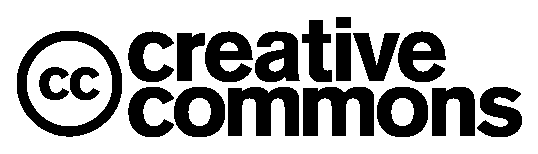
\includegraphics[width=0.8\textwidth]{title_images/cc2.eps}
\end{minipage}
\begin{minipage}{0.3\textwidth}
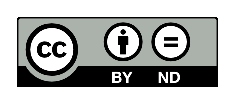
\includegraphics[width=0.8\textwidth]{title_images/cc1.eps}
\end{minipage}
\end{center}

% Authors
\newpage
\thispagestyle{empty}


\begin{flushleft} \textbf{\huge Authors List} \end{flushleft}

{\LARGE This book is based upon the original Free High School Science Text which was entirely written by
volunteer academics, educators and industry professionals. Their vision was to see a curriculum aligned
set of mathematics and physical science textbooks which are freely available to anybody and exist
under an open copyright license.} \par

\textbf{\LARGE Siyavula core team} \\

Neels van der Westhuizen; Alison Jenkin; Marina van Zyl; Helen Robertson; Carl Scheffler; Nicola du Toit; Leonard Gumani Mudau; \par

\textbf{\LARGE Original Free High School Science Texts core team}\\

Mark Horner; Samuel Halliday; Sarah Blyth; Rory Adams; Spencer Wheaton \par 


\textbf{\LARGE Original Free High School Science Texts editors}\\

Jaynie Padayachee; Joanne Boulle; Diana Mulcahy; Annette Nell; René Toerien; Donovan Whitfield \par

\textbf{\LARGE Siyavula and Free High School Science Texts contributors}\\

    Sarah Abel;
Dr. Rory Adams;
    Andrea Africa;
    Matthew Amundsen;
    Ben Anhalt;
    Prashant Arora;
    Amos Baloyi;
    Bongani Baloyi;
    Raymond Barbour;
    Caro-Joy Barendse;
    Richard Baxter;
    Tara Beckerling;
Dr. Sarah Blyth;
    Sebastian Bodenstein;
    Martin Bongers;
    Gareth Boxall;
    Stephan Brandt;
    Hannes Breytenbach;
    Alex Briell;
    Wilbur Britz;
    Graeme Broster;
    Craig Brown;
    Richard Burge;
    Bianca Böhmer;
    George Calder-Potts;
    Eleanor Cameron;
    Richard Case;
    Sithembile Cele;
    Alice Chang;
    Richard Cheng;
    Fanny Cherblanc;
Dr. Christine Chung;
    Brett Cocks;
    Stefaan Conradie;
    Rocco Coppejans;
    Tim Craib;
    Andrew Craig;
    Tim Crombie;
    Dan Crytser;
Dr. Anne Dabrowski;
    Laura Daniels;
    Gareth Davies;
    Jennifer de Beyer;
    Jennifer de Beyer;
    Deanne de Bude;
    Mia de Vos;
    Sean Dobbs;
    Buhle Donga;
    William Donkin;
    Esmi Dreyer;
    Nicola du Toit;
    Matthew Duddy;
    Fernando Durrell;
Dr. Dan Dwyer;
    Alex Ellis;
    Tom Ellis;
    Andrew Fisher;
    Giovanni Franzoni;
    Nina Gitau Muchunu;
    Lindsay Glesener;
    Kevin Godby;
Dr. Vanessa Godfrey;
    Terence Goldberg;
Dr. Johan Gonzalez;
    Saaligha Gool;
    Hemant Gopal;
Dr. Stephanie Gould;
    Umeshree Govender;
    Heather Gray;
    Lynn Greeff;
    Carine Grobbelaar;
Dr. Tom Gutierrez;
    Brooke Haag;
    Kate Hadley;
    Alex Hall;
Dr. Sam Halliday;
    Asheena Hanuman;
Dr. Nicholas Harrison;
    Neil Hart;
    Nicholas Hatcher;
    Jason Hayden;
    Laura Hayward;
    Cho Hee Shrader;
Dr. Fritha Hennessy;
    Shaun Hewitson;
    Millie Hilgart;
    Grant Hillebrand;
    Nick Hobbs;
    Chris Holdsworth;
Dr. Benne Holwerda;
Dr. Mark Horner;
    Robert Hovden;
    Mfandaidza Hove;
    Jennifer Hsieh;
    Laura Huss;
Dr. Matina J. Rassias;
    Rowan Jelley;
    Grant Jelley;
    Clare Johnson;
    Luke Jordan;
    Tana Joseph;
Dr. Fabian Jutz;
    Brian Kamanzi;
Dr. Lutz Kampmann;
    Simon Katende;
    Natalia Kavalenia;
    Nothando Khumalo;
    Paul Kim;
Dr. Jennifer Klay;
    Lara Kruger;
    Sihle Kubheka;
    Andrew Kubik;
Dr. Jannie Leach;
    Nkoana Lebaka;
Dr. Tom Leinster;
    Henry Liu;
    Christopher Loetscher;
    Mike Loseby;
    Amandla Mabona;
    Malothe Mabutho;
    Stuart Macdonald;
Dr. Anton Machacek;
    Tshepo Madisha;
    Batsirai Magunje;
Dr. Komal Maheshwari;
    Michael Malahe;
    Masoabi Malunga;
    Masilo Mapaila;
    Bryony Martin;
    Nicole Masureik;
    John Mathew;
Dr. Will Matthews;
    Chiedza Matuso;
    JoEllen McBride;
    Dr Melanie Dymond Harper;
    Nikolai Meures;
    Riana Meyer;
    Filippo Miatto;
    Jenny Miller;
    Abdul Mirza;
    Mapholo Modise;
    Carla Moerdyk;
    Tshwarelo Mohlala;
    Relebohile Molaoa;
    Marasi Monyau;
    Asogan Moodaly;
    Jothi Moodley;
    Robert Moon;
    Calvin Moore;
    Bhavani Morarjee;
    Kholofelo Moyaba;
    Kate Murphy;
    Emmanuel Musonza;
    Tom Mutabazi;
    David Myburgh;
    Kamie Naidu;
    Nolene Naidu;
    Gokul Nair;
    Vafa Naraghi;
    Bridget Nash;
    Tyrone Negus;
    Huw Newton-Hill;
    Buntu Ngcebetsha;
Dr. Markus Oldenburg;
    Thomas O’Donnell;
Dr. William P. Heal;
Dr. Jaynie Padayachee;
    Poveshen Padayachee;
    Masimba Paradza;
    Dave Pawson;
    Justin Pead;
    Nicolette Pekeur;
    Sirika Pillay;
    Jacques Plaut;
    Barry Povey;
    Barry Povey;
    Andrea Prinsloo;
    Joseph Raimondo;
    Sanya Rajani;
    Alastair Ramlakan;
Dr. Jocelyn Read;
    Jonathan Reader;
    Jane Reddick;
Dr. Matthew Reece;
    Razvan Remsing;
    Laura Richter;
    Max Richter;
    Sean Riddle;
Dr. David Roberts;
    Christopher Roberts;
    Helen Robertson;
    Evan Robinson;
    Raoul Rontsch;
Dr. Andrew Rose;
    Katie Ross;
    Jeanne-Marié Roux;
    Mark Roux;
    Bianca Ruddy;
    Nitin Rughoonauth;
    Katie Russell;
    Steven Sam;
Dr. Carl Scheffler;
    Nathaniel Schwartz;
    Duncan Scott;
    Helen Seals;
    Relebohile Sefako;
    Prof. Sergey Rakityansky;
    Sandra Serumaga-Zake;
    Paul Shangase;
    Cameron Sharp;
    Ian Sherratt;
Dr. James Short;
    Roger Sieloff;
    Brandon Sim;
    Bonga Skozana;
    Clare Slotow;
    Bradley Smith;
    Greg Solomon;
    Nicholas Spaull;
Dr. Andrew Stacey;
Dr. Jim Stasheff;
    Mike Stay;
    Mike Stringer;
    Masixole Swartbooi;
    Tshenolo Tau;
    Tim Teatro;
    Ben Tho.epson;
    Shen Tian;
    Xolani Timbile;
    Robert Torregrosa;
    Jimmy Tseng;
    Tim van Beek;
    Neels van der Westhuizen;
    Frans van Eeden;
    Pierre van Heerden;
Dr. Marco van Leeuwen;
    Marina van Zyl;
    Pieter Vergeer;
    Rizmari Versfeld;
    Mfundo Vezi;
    Mpilonhle Vilakazi;
    Ingrid von Glehn;
    Tamara von Glehn;
    Kosma von Maltitz;
    Helen Waugh;
    Leandra Webb;
Dr. Dawn Webber;
    Michelle Wen;
Dr. Alexander Wetzler;
Dr. Spencer Wheaton;
    Vivian White;
Dr. Gerald Wigger;
    Harry Wiggins;
    Heather Williams;
    Wendy Williams;
    Julie Wilson;
    Timothy Wilson;
    Andrew Wood;
    Emma Wormauld;
Dr. Sahal Yacoob;
    Jean Youssef;
    Ewald Zietsman 







% Everything Maths page
\newpage
\thispagestyle{empty}

{\normalfont\sffamily\fontsize{22}\normalfont\itshape Everything Maths} \par

{ \Large
Mathematics is commonly thought of as being about numbers but mathematics is actually a language! Mathematics is the language that nature speaks to us in. As we learn to understand and speak this language, we can discover many of nature’s secrets. Just as understanding someone’s language is necessary to learn more about them, mathematics is required to learn about all aspects of the world -- whether it is physical sciences, life sciences or even finance and economics.\par


The great writers and poets of the world have the ability to draw on words and put them together in
ways that can tell beautiful or inspiring stories. In a similar way, one can draw on mathematics to
explain and create new things. Many of the modern technologies that have enriched our lives are
greatly dependent on mathematics. DVDs, Google searches, bank cards with PIN numbers are just
some examples. And just as words were not created specifically to tell a story but their existence enabled
stories to be told, so the mathematics used to create these technologies was not developed for its own sake,
but was available to be drawn on when the time for its application was right.\par


There is in fact not an area of life that is not affected by mathematics. Many of the most sought after
careers depend on the use of mathematics. Civil engineers use mathematics to determine how to best
design new structures; economists use mathematics to describe and predict how the economy will react
to certain changes; investors use mathematics to price certain types of shares or calculate how risky
particular investments are; software developers use mathematics for many of the algorithms (such as
Google searches and data security) that make programmes useful.\par



But, even in our daily lives mathematics is everywhere – in our use of distance, time and money.
Mathematics is even present in art, design and music as it informs proportions and musical tones. The
greater our ability to understand mathematics, the greater our ability to appreciate beauty and
everything in nature. Far from being just a cold and abstract discipline, mathematics
embodies logic, symmetry, harmony and technological progress. More than any other language,
mathematics is everywhere and universal in its application.\par


See introductory video by Dr. Mark Horner: \raisebox{-0.2em}{
\includegraphics[height=1em]{../../icons/video.ps}} VMiwd at www.everythingmaths.co.za



}





% Webbook page

\newpage
\thispagestyle{empty}

{\normalfont\sffamily\fontsize{22}\normalfont\itshape More than a regular textbook} \par

\begin{center}
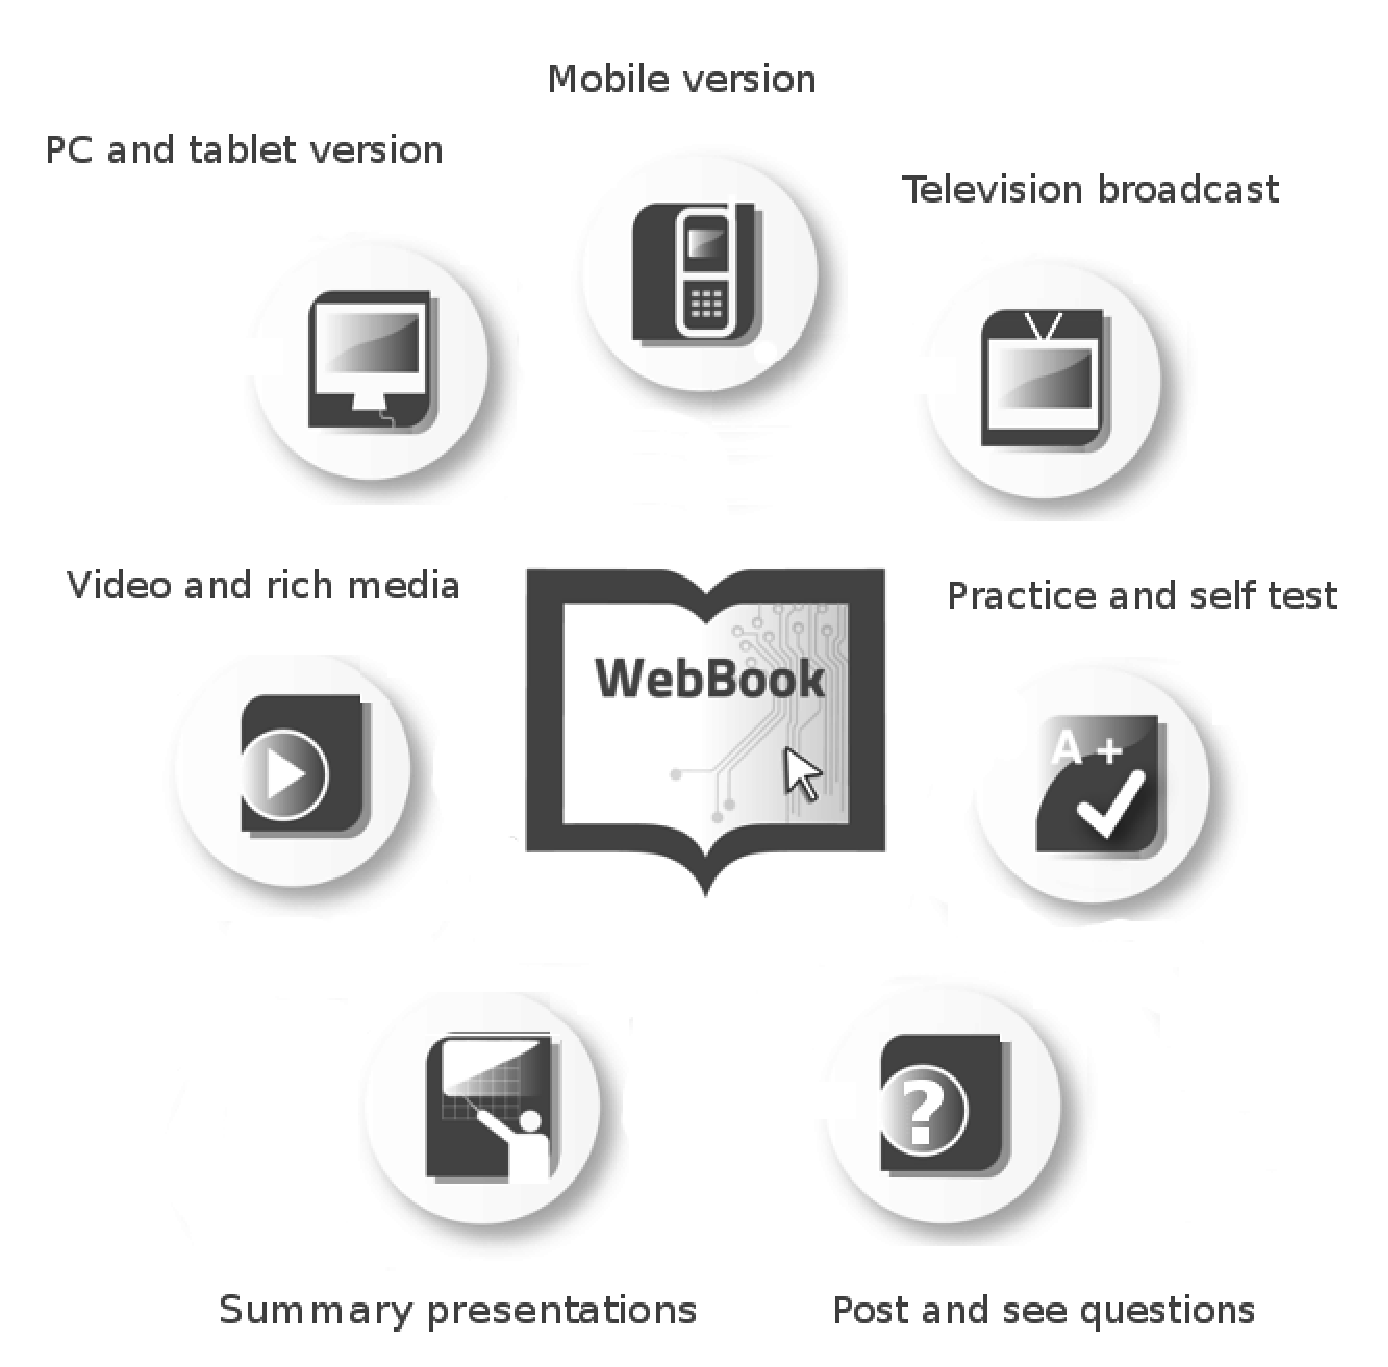
\includegraphics[width=0.70\textwidth]{title_images/morethantextbook.eps}
\end{center}

\par
{\Large
\textbf{\textit{Everything Maths}} is not just a Mathematics textbook. It has everything you expect from
your regular printed school textbook, but comes with a whole lot more. For a start, you can download or read it
on-line on your mobile phone, computer or iPad, which means you have the convenience of accessing
it wherever you are.\par


We know that some things are hard to explain in words. That is why every chapter comes with video
lessons and explanations which help bring the ideas and concepts to life. Summary presentations at
the end of every chapter offer an overview of the content covered, with key points highlighted for easy
revision.\par


All the exercises inside the book link to a service where you can get more practice, see the full solution
or test your skills level on mobile and PC.\par


We are interested in what you think, wonder about or struggle with as you read through the book and
attempt the exercises. That is why we made it possible for you to use your mobile phone or computer to
digitally pin your question to a page and see what questions and answers other readers pinned up.\par


% This book is the same one used by Mindset Learn in their new television broadcast, where experienced educators work through it, explain the concepts and work out exercises from the book.
}




% mobile or PC
\newpage
\thispagestyle{empty}

{\normalfont\sffamily\fontsize{22}\normalfont\itshape Everything Maths on your mobile or PC} \par

{\Large
You can have this textbook at hand wherever you are – whether at home, on the the train or at school.
Just browse to the on-line version of Everything Maths on your mobile phone, tablet or computer. To
read it off-line you can download a PDF or e-book version.\par


To read or download it, go to \textbf{www.everythingmaths.co.za} on your phone or computer.} \vspace*{2cm}


\begin{center}
\begin{minipage}{0.4\textwidth}
\centering
\includegraphics[width=0.8\textwidth]{title_images/ipad.eps}
\end{minipage}
\begin{minipage}{0.4\textwidth}
\centering
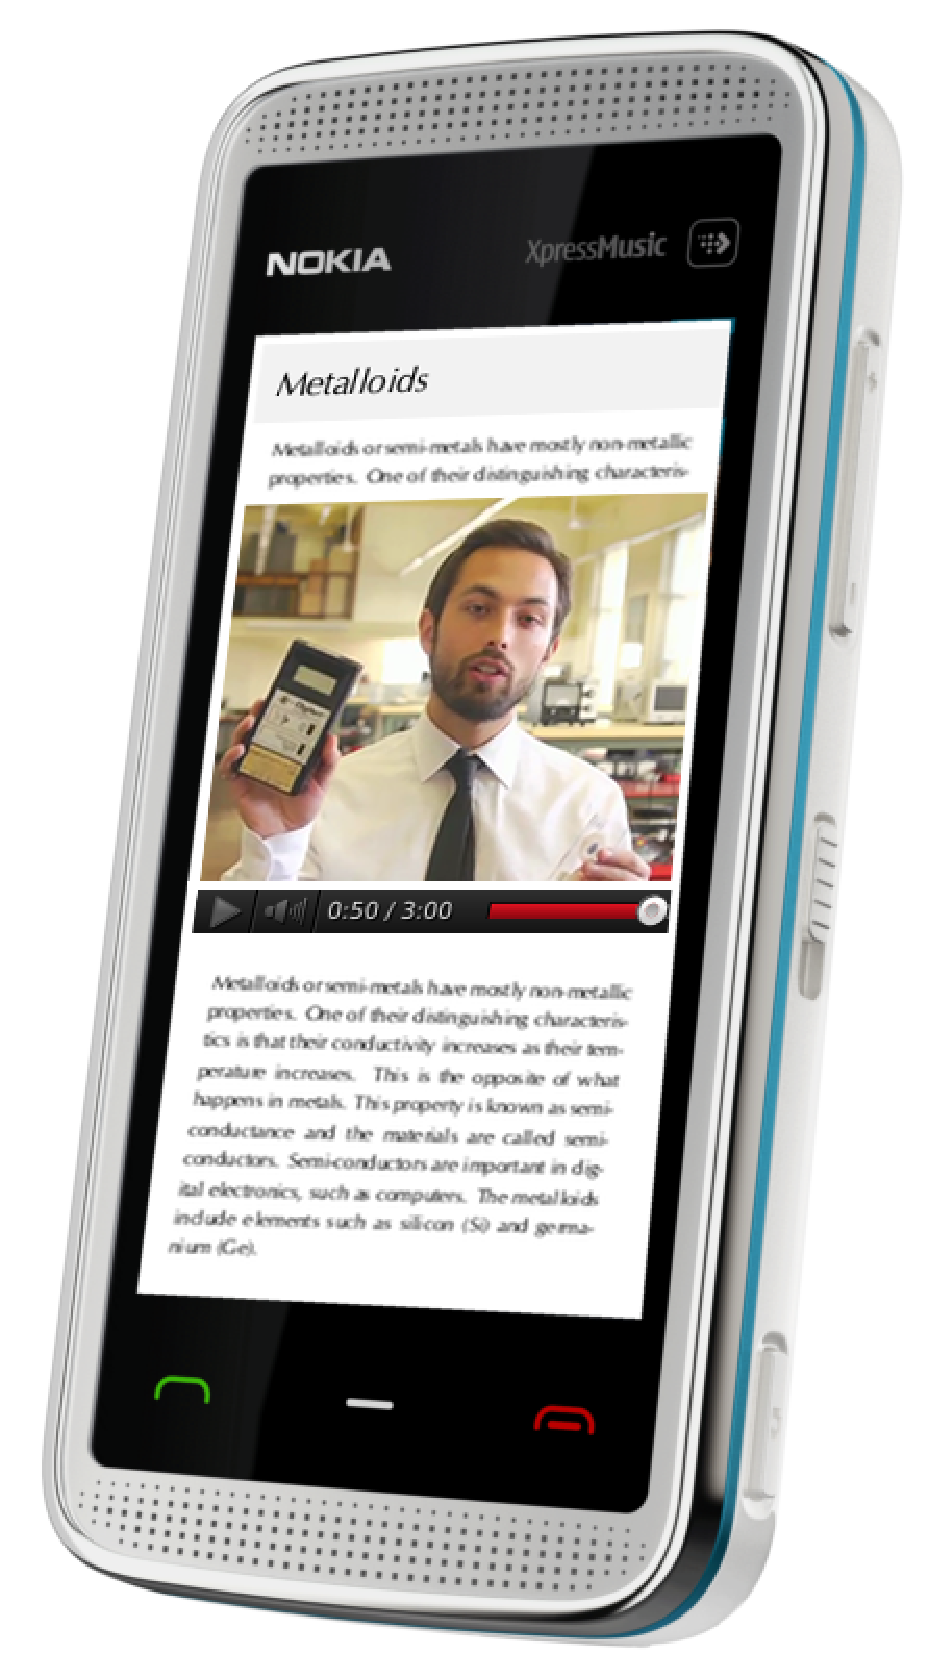
\includegraphics[width=0.4\textwidth]{title_images/phone.eps}
\end{minipage}
\end{center}

\vspace*{2cm}


{\normalfont\sffamily\fontsize{22}\normalfont\itshape Using the icons and short-codes} \par

{\Large
Inside the book you will find these icons to help you spot where videos, presentations, practice tools
and more help exist. The short-codes next to the icons allow you to navigate directly to the resources
on-line without having to search for them.\par


\begin{tabular}{lcl}
\raisebox{-0.8em}{
\includegraphics[width=0.8cm]{../../icons/www.ps}} & (A123) & Go directly to a section \\
\raisebox{-0.8em}{
\includegraphics[width=0.8cm]{../../icons/video.ps}} & (V123) & Video, simulation or presentation \\
\raisebox{-0.8em}{
\includegraphics[width=0.8cm]{../../icons/aplus.ps}} & (P123) & Practice and test your skills \\
\raisebox{-0.8em}{
\includegraphics[width=0.8cm]{../../icons/help.ps}} & (Q123) & Ask for help or find an answer \\
\end{tabular}
\par
\vspace*{1cm}

To watch the videos on-line, practise your skills or post a question, go to the \textit{Everything Maths} website at \textbf{www.everythingmaths.co.za} on your mobile or PC and enter the short-code in the navigation box.
}




% video lessons
\newpage
\thispagestyle{empty}

{\normalfont\sffamily\fontsize{22}\normalfont\itshape Video lessons} \par

{\Large

Look out for the video icons inside the book. These will take you to video lessons that help bring the ideas and concepts on the page to life. Get extra insight, detailed
explanations and worked examples. See the concepts in action and hear real people talk about how they
use maths and science in their work. \par

\begin{figure}[h]
\begin{center}
See video explanation \raisebox{-0.6em}{
\includegraphics[width=0.7cm]{../../icons/video.ps}} (Video: V123)\\
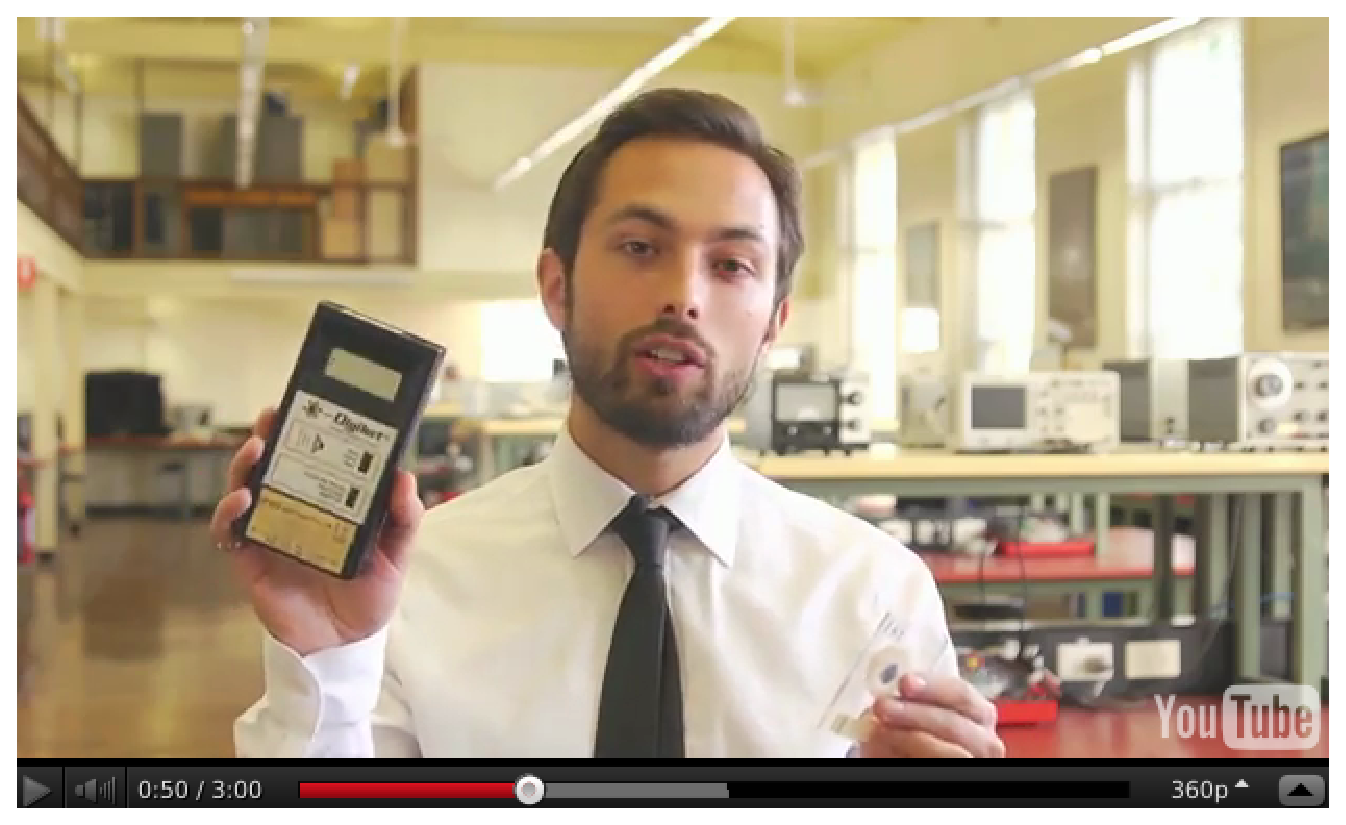
\includegraphics[width=0.5\textwidth]{title_images/veritasiumvideo.eps}
\end{center}
\end{figure}

}
\vspace{0.5cm}
{\normalfont\sffamily\fontsize{22}\normalfont\itshape Video exercises} \par

{\Large

Wherever there are exercises in the book you will see icons and short-codes for video solutions,
practice and help. These short-codes will take you to video solutions of select exercises to show you
step-by-step how to solve such problems. \par

\begin{figure}[h]
\begin{center}
See video exercise \raisebox{-0.6em}{
\includegraphics[width=0.7cm]{../../icons/video.ps}} (Video: V123)\\ 
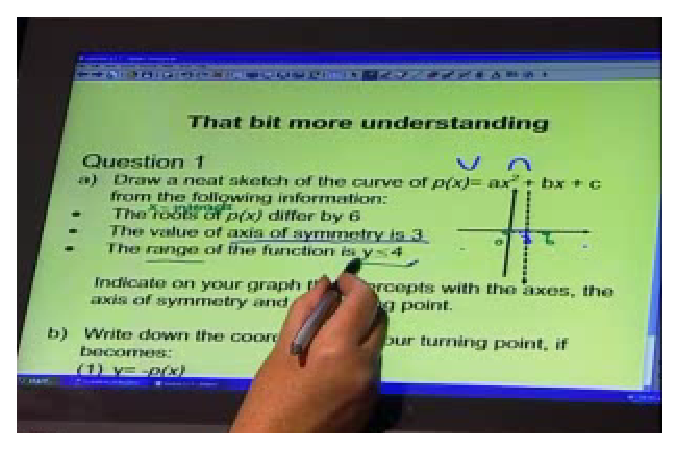
\includegraphics[width=0.5\textwidth]{title_images/mindsetexercise.eps}
\end{center}
\end{figure}
You can get these videos by:
\begin{itemize}
    \item viewing them on-line on your mobile or computer
    \item downloading the videos for off-line viewing on your phone or computer
    \item ordering a DVD to play on your TV or computer
    \item downloading them off-line over Bluetooth or Wi-Fi from select outlets
\end{itemize}
}


% practise and test your skills
\newpage
\thispagestyle{empty}
{\Large

To view, download, or for more information, visit the Everything Maths website on your phone or
computer at \underline{www.everythingmaths.co.za}  \par
\vspace*{1cm}
{\normalfont\sffamily\fontsize{22}\normalfont\itshape Practice and test your skills} \par


One of the best ways to prepare for your tests and exams is to practice answering the same kind of
questions you will be tested on. At every set of exercises you will see a practice icon and short-code.
This on-line practice for \textbf{mobile} and \textbf{PC} will keep track of your performance and progress, give you
feedback on areas which require more attention and suggest which sections or videos to look at.

\begin{figure}[h]
\begin{center}
See more practice \raisebox{-0.6em}{
\includegraphics[width=0.7cm]{../../icons/aplus.ps}} (QM123)\\ 
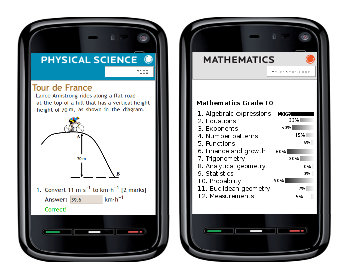
\includegraphics[width=0.65\textwidth]{title_images/practicephones.eps}
\end{center}
\end{figure}
\par



To practice and test your skills:\par

Go to \underline{www.everythingmaths.co.za} on your mobile phone or PC and enter the short-code.\par

\vspace*{1cm}


%{\normalfont\sffamily\fontsize{22}\normalfont\itshape Television broadcasts} \par
%This book is the same one used by \textbf{Mindset Learn} in their television broadcast where experienced
%educators explain the key concepts, perform live experiments and work out exercises from the book.
%\textbf{Mindset Learn} broadcasts a full 28 hours of curriculum support each week of term. \par
%
%
%Maths can be seen on Mondays and Science on Tuesdays. There is also Life Sciences on Wednesdays
%and Maths Literacy on Thursdays. Revision of the week's work is done on Saturdays for Grade 12 and on
%Sundays for Grades 10 and 11.


}



% video lessons
\newpage
\thispagestyle{empty}

{\normalfont\sffamily\fontsize{22}\normalfont\itshape Ask questions and find answers} \par

{\Large

Have you ever had a question about a specific fact, formula or exercise in your textbook and wished you could just ask someone? Surely someone else in the country must have had the same question at the same place in the textbook.\par 

We invite you to open the textbook on your mobile phone or computer and pin your question at that  exact spot in the textbook using the shortcode. You will be able to see whether it has been asked before and what the given answer to that question is. \par

The short codes at section headings helps you navigate to sections in the book to ask and view questions for that section. The short codes for the exercises lets you look at questions and answers relating to those specific exercises.\par

\begin{tabular}{lcl}
\raisebox{-0.8em}{
\includegraphics[width=0.8cm]{../../icons/www.ps}} & (A123) & Visit this section to post or view questions\\
\raisebox{-0.8em}{
\includegraphics[width=0.8cm]{../../icons/help.ps}} & (Q123) & Questions or help with a specific question  \\
\end{tabular}



\begin{figure}[h]
\centering
\includegraphics[width=\textwidth]{title_images/questions.eps}
\end{figure}


}

%% practise and test your skills
%\newpage
%\thispagestyle{empty}
%{\Large
%
%\begin{table*}[h]
%\large
%\begin{tabular}{lll}
%\textbf{Maths and Science Broadcasts}&&\\
%Grade 10  Maths & Mondays at 4pm & Every second Sunday at 1pm\\
%Grade 11  Maths & Mondays at 5pm & Every second Sunday at 9am\\
%Grade 12  Maths & Mondays at 6pm & Every Saturday at 9am\\
%Grade 10  Science & Tuesdays at 4pm & Every second Sunday at 1pm\\
%Grade 11  Science & Tuesdays at 5pm & Every second Sunday at 9am\\
%Grade 12  Science & Tuesdays at 6pm & Every Saturday at 11am\\
%\textbf{Other broadcasts} & & \\
%Grade 10  Life Science & Wednesdays at 4pm & Every second Sunday at 3pm\\
%Grade 11  Life Science & Wednesdays at 5pm & Every second Sunday at 9am\\
%Grade 12  Life Science & Wednesdays at 6pm & Every Saturday at 1pm\\
%Grade 10  Maths Literacy & Thursdays at 4pm & Every second Sunday at 3pm\\
%Grade 11  Maths Literacy & Thursdays at 5pm & Every second Sunday at 9am\\
%Grade 12  Maths Literacy & Thursdays at 6pm & Every Saturday at 3pm\\
%\end{tabular}
%\end{table*}
%
%
%\textbf{You can watch these live sessions on:}
%\begin{itemize}
%    \item Mindset free-to-air for schools (ask your school)
%    \item Channels 319 on DStv
%    \item Toptv on 319 on TopTV
%\end{itemize}


%}

% Put the margins back for the rest of the book



\tableofcontents
\pagenumbering{arabic}

% change shortcodeprefix to the correct value
\renewcommand{\shortcodeprefix}{EMC}

\newgeometry{lmargin=0.1\paperwidth, rmargin=0.25\paperwidth, tmargin=1in, bmargin=1in, twoside, centering, includehead,  marginparwidth=0.225\paperwidth}
\normalfont

 \chapter{Introduction to Book}
\label{mathintro}

\section{The Language of Mathematics}
The purpose of any language, like English or Zulu, is to make it possible for people to communicate. All languages have an alphabet, which is a group of letters that are used to make up words. There are also rules of grammar which explain how words are supposed to be used to build up sentences. This is needed because when a sentence is written, the person reading the sentence understands exactly what the writer is trying to explain. Punctuation marks (like a full stop or a comma) are used to further clarify what is written.

Mathematics is a language, specifically it is the language of Science. Like any language, mathematics has letters (known as numbers) that are used to make up words (known as expressions), and sentences (known as equations). The punctuation marks of mathematics are the different signs and symbols that are used, for example, the plus sign ($+$), the minus sign ($-$), the multiplication sign ($\times$), the equals sign ($=$) and so on. There are also rules that explain how the numbers should be used together with the signs to make up equations that express some meaning.


 \chapter{Logarithms}
\label{m:f12:logarithms}

%\begin{syllabus}
%\item Demonstrate an understanding of the definition of a logarithm and any laws needed to solve real-life problems (e.g. growth and decay or $A=P(1\pm i)^n$).
%\end{syllabus}

\section{Introduction}

In mathematics many ideas are related. We saw that addition and subtraction are related and that multiplication and division are related. Similarly, exponentials and logarithms are related. 

\textit{Logarithms}, commonly referred to as \textit{logs}, are the inverse of exponentials. The logarithm of a number $x$ in the base $a$ is defined as the number $n$ such that $a^n = x$. 

So, if $a^n = x$, then:
\begin{equation}
\label{eq:mn:l}
\log_{a}(x) = n
\end{equation}

%\Extension{Inverse Function}{When we say ``inverse function'' we mean that the answer becomes the
%question and the question becomes the answer. For example, in the equation $a^{b} = x$ the
%``question'' is ``what is $a$ raised to the power $b$?'' The answer is ``$x$.'' The inverse function
%would be $\log_{a}x=b$ or ``by what power must we raise $a$ to obtain $x$?'' The answer is ``$b$.'' }
%
%The mathematical symbol for logarithm is $\log_{a}(x)$ and it is read ``log to the base $a$ of $x$''. For example, $\log_{10}(100)$ is ``log to the base $10$of $100$.''
%
\chapterstartvideo{VMgio}

\section{Definition of Logarithms}
The logarithm of a number is the value to which the base must be raised to give that number i.e.\@{} the exponent.  From the first example of the activity $\log_{2}(4)$ means the power of $2$ that will give $4$.  As $2^2=4$, we see that
\begin{equation} 
\log_{2}(4) = 2
\end{equation}
The \textit{exponential-form} is then $2^2 = 4$  and the \textit{logarithmic-form} is $\log_{2}4=2$.
\Definition{Logarithms}{If $a^n = x$, then: $\log_{a}(x) = n$, where $a>0$; $a \neq1$ and $x>0$.}

\Activity{}{Logarithm Symbols}{Write the following out in words. The first one is done for you.
\begin{enumerate}
\item $\log_{2}(4)$ is log to the base $2$ of $4$
\item $\log_{10}(14)$
\item $\log_{16}(4)$
\item $\log_{x}(8)$
\item $\log_{y}(x)$
\end{enumerate}}

\Activity{}{Applying the definition}{Find the value of:
\begin{enumerate}
\item{$\log_{7}343$}
\begin{eqnarray*}
\rm{Reasoning:}\\
7^3 = 343\\
\rm{therefore,~} \log_{7}343 = 3
\end{eqnarray*}
\item{$\log_{2}8$}
\item{$\log_{4}\frac{1}{64}$}
\item{$\log_{10}1~000$}
\end{enumerate}}

\section{Logarithm Bases}
Logarithms, like exponentials, also have a base and $\log_{2}(2)$ is not the same as $\log_{10}(2)$. 

We generally use the ``common'' base, $10$, or the \textit{natural} base, $e$.

The number $e$ is an irrational number between $2.71$ and $2.72$. It comes up surprisingly often in Mathematics, but for now suffice it to say that it is one of the two common bases.

\Extension{Natural Logarithm}{The natural logarithm (symbol $\ln$) is widely used in the sciences.
The natural logarithm is to the base $e$ which is approximately $2.71828183\ldots$. $e$, like $\pi$
and is an example of an irrational number.}

While the notation $\log_{10}(x)$ and $\log_{e}(x)$ may be used, $\log_{10}(x)$ is often written $\log(x)$ in Science and $\log_{e}(x)$ is normally written as $\ln(x)$ in both Science and Mathematics. So, if you see the $\log$ symbol without a base, it means $\log_{10}$.

It is often necessary or convenient to convert a log from one base to another. An engineer might need an approximate solution to a log in a base for which he does not have a table or calculator function, or it may be algebraically convenient to have two logs in the same base.

Logarithms can be changed from one base to another, by using the change of base formula:
\begin{equation}
\label{eq:mf:a:basechange}
\log_{a}x=\frac{\log_{b}x}{\log_{b}a}
\end{equation}
where $b$ is any base you find convenient. Normally $a$ and $b$ are known,
therefore $\log_{b}a$ is normally a known, if irrational, number.

For example, change $\log_{2}12$ in base $10$ is:
\begin{equation*}
\log_{2}12=\frac{\log_{10}12}{\log_{10}2}
\end{equation*}

\Activity{}{Change of Base}{Change the following to the indicated base:
\begin{enumerate}
\item{$\log_{2}(4)$ to base $8$}
\item{$\log_{10}(14)$ to base $2$}
\item{$\log_{16}(4)$ to base $10$}
\item{$\log_{x}(8)$ to base $y$}
\item{$\log_{y}(x)$ to base $x$}
\end{enumerate}}
% Khan Academy video on logarithms:SIYAVULA-VIDEO:http://cnx.org/content/m31883/latest/#logs-1
\mindsetvid{Khan on logs}{VMgiq}
\section{Laws of Logarithms}
Just as for the exponents, logarithms have some laws which make working with them easier. These laws are based on the exponential laws and are summarised first and then explained in detail.

\begin{eqnarray}
\label{eq:mn:l:law1}
\log_{a}(1)&=&0\\
\label{eq:mn:l:law2}
\log_{a}(a)&=&1 \\
\label{eq:mn:l:law3}
\log_{a}(x\,.\, y) &=& \log_{a}(x) + \log_{a}(y)\\
\label{eq:mn:l:law4}
\log_{a}\left(\frac{x}{y}\right) &=& \log_{a}(x) - \log_{a}(y) \\
\label{eq:mn:l:law5}
\log_{a}(x^b) &=& b \log_{a}(x)\\
\label{eq:mn:l:law6}
\log_{a}\left(\sqrt[b]{x}\right) &=& \frac{\log_{a}(x)}{b}
\end{eqnarray}

\section{Logarithm Law 1: $\log_{a}1 = 0$}
\begin{eqnarray*}
\mbox{Since}\quad a^0&=&1\\
\mbox{Then,}\quad \log_{a}(1)&=&0\qquad \mbox{by definition of logarithm in Equation~\ref{eq:mn:l}}
\end{eqnarray*}

For example,
\nequ{\log_2 1 = 0}
and
\nequ{\log_{25} 1 = 0}

\Activity{}{Logarithm Law 1: $\log_{a}1 = 0$}{Simplify the following:
\begin{enumerate}
\item{$\log_{2}(1)+5$}
\item{$\log_{10}(1)\times 100$}
\item{$3\times\log_{16}(1)$}
\item{$\log_{x}(1)+2xy$}
\item{$\frac{\log_{y}(1)}{x}$}
\end{enumerate}}

\section{Logarithm Law 2: $\log_{a}(a) = 1$}
\begin{eqnarray*}
\mbox{Since}\quad a^1&=&a\\
\mbox{Then,}\quad \log_{a}(a) &=&1\qquad \mbox{by definition of logarithm in Equation~\ref{eq:mn:l}}
\end{eqnarray*}

For example,
\nequ{\log_2 2 = 1}
and
\nequ{\log_{25} 25 = 1}

\Activity{}{Logarithm Law 2: $\log_{a}(a) = 1$}{Simplify the following:
\begin{enumerate}
\item{$\log_{2}(2)+5$}
\item{$\log_{10}(10)\times 100$}
\item{$3\times\log_{16}(16)$}
\item{$\log_{x}(x)+2xy$}
\item{$\frac{\log_{y}(y)}{x}$}
\end{enumerate}}

\Tip{Useful to know and remember}{\textit{When the base is $10$ we do not need to state it.} 
From the work done up to now, it is also useful to summarise the following facts:
\begin{enumerate}
\item{$\log 1 = 0$}
\item{$\log 10 = 1$}
\item{$\log 100 = 2$}
\item{$\log 1000 = 3$}
\end{enumerate}}

\section{Logarithm Law 3: $\log_{a}(x\,.\, y) = \log_{a}(x) + \log_{a}(y)$}
The derivation of this law is a bit trickier than the first two. Firstly, we need to relate $x$ and $y$ to the base $a$. So, assume that $x=a^m$ and $y=a^n$. Then from Equation~\ref{eq:mn:l}, we have that:
\begin{eqnarray}
\label{eq:mn:loglaw3:1}
\log_{a}(x) &=&m\\
\label{eq:mn:loglaw3:2}
\mbox{and}\quad \log_{a}(y) &=&n
\end{eqnarray}

This means that we can write:
\begin{eqnarray*}
\log_{a}(x \,.\, y)&=&\log_{a}(a^m \,.\, a^n)\\
&=&\log_{a}(a^{m+n}) \qquad \mbox{(Exponential Law Equation (Grade 10))}\\
&=&\log_{a}(a^{\log_{a}(x)+\log_{a}(y)}) \qquad \mbox{(From Equation~\ref{eq:mn:loglaw3:1} and Equation~\ref{eq:mn:loglaw3:2})}\\
&=&\log_{a}(x)+\log_{a}(y) \qquad \mbox{(From Equation~\ref{eq:mn:l})}
\end{eqnarray*}

For example, show that $\log (10 \,.\, 100) = \log 10 + \log 100$. Start with calculating the left hand side:
\begin{eqnarray*}
\log (10 \,.\, 100) &=& \log (1000)\\
&=& \log (10^3)\\
&=&3
\end{eqnarray*}
The right hand side:
\begin{eqnarray*}
\log 10 + \log 100 &=& 1 + 2\\
&=&3
\end{eqnarray*}
Both sides are equal. Therefore, $\log (10 \,.\, 100) = \log 10 + \log 100$.

\Activity{}{Logarithm Law 3: $\log_{a}(x\,.\, y) = \log_{a}(x) + \log_{a}(y)$}{Write as separate logs:
\begin{enumerate}
\item{$\log_{2}(8\times4)$}
\item{$\log_{8}(10\times10)$}
\item{$\log_{16}(xy)$}
\item{$\log_{z}(2xy)$}
\item{$\log_{x}(y^2)$}
\end{enumerate}}

\section[Logarithm Law 4: $\log_{a}\left(\frac{x}{y}\right) = \log_{a}(x) - \log_{a}(y)$]{Logarithm Law 4: \Huge $\log_{a}\left(\frac{x}{y}\right) = \log_{a}(x) - \log_{a}(y)$}

The derivation of this law is identical to the derivation of Logarithm Law 3 and is left as an exercise.

For example, show that $\log (\frac{10}{100}) = \log 10 - \log 100$. Start with calculating the left hand side:
\begin{eqnarray*}
\log \left(\frac{10}{100}\right) &=& \log \left(\frac{1}{10}\right)\\
&=& \log (10^{-1})\\
&=&-1
\end{eqnarray*}
The right hand side:
\begin{eqnarray*}
\log 10 - \log 100 &=& 1 -2 \\
&=&-1
\end{eqnarray*}
Both sides are equal. Therefore, $\log (\frac{10}{100}) = \log 10 - \log 100$.

\Activity{}{Logarithm Law 4: $\log_{a}\left(\frac{x}{y}\right) = \log_{a}(x) - \log_{a}(y)$}{Write as separate logs:
\begin{enumerate}
\item{$\log_{2}(\frac{8}{5})$}
\item{$\log_{8}(\frac{100}{3})$}
\item{$\log_{16}(\frac{x}{y})$}
\item{$\log_{z}(\frac{2}{y})$}
\item{$\log_{x}(\frac{y}{2})$}
\end{enumerate}}

\section{Logarithm Law 5: $\log_{a}(x^b) = b \log_{a}(x)$}
Once again, we need to relate $x$ to the base $a$. So, we let $x=a^m$. Then,
\begin{eqnarray*}
\log_{a}(x^b)&=&\log_{a}((a^m)^b)\\
&=&\log_{a}(a^{m \,.\, b}) \quad \mbox{(Exponential Law in Equation (Grade 10))}\\
\mbox{But,}\quad m &=& \log_{a}(x)\quad \quad \mbox{(Assumption that $x=a^m$)}\\
\therefore \quad \log_{a}(x^b)&=&\log_{a}(a^{b \,.\, \log_{a}(x)})\\
&=&b \,.\, \log_{a}(x) \quad \mbox{(Definition of logarithm in Equation~\ref{eq:mn:l})}
\end{eqnarray*}

For example, we can show that $\log_{2}(5^3) = 3 \log_{2}(5)$.
\begin{eqnarray*}
\log_{2}(5^3) &=& \log_2 (5 \,.\, 5 \,.\, 5)\\
&=& \log_2 5 + \log_2 5 + \log_2 5\quad (\because \log_{a}(x \,.\, y)=\log_{a}(a^m \,.\, a^n))\\
&=&3 \log_2 5
\end{eqnarray*}
Therefore, $\log_{2}(5^3) = 3 \log_{2}(5)$.

\Activity{}{Logarithm Law 5: $\log_{a}(x^b) = b \log_{a}(x)$}{Simplify the following:
\begin{enumerate}
\item{$\log_{2}(8^4)$}
\item{$\log_{8}(10^{10})$}
\item{$\log_{16}(x^y)$}
\item{$\log_{z}(y^x)$}
\item{$\log_{x}(y^{2x})$}
\end{enumerate}}

\section{Logarithm Law 6: $\log_{a}\left(\sqrt[b]{x}\right) = \frac{\log_{a}(x)}{b}$}

The derivation of this law is identical to the derivation of Logarithm Law 5 and is left as an exercise.

For example, we can show that $\log_{2}(\sqrt[3]{5}) = \frac{\log_{2}5}{3} $.
\begin{eqnarray*}
\log_{2}(\sqrt[3]{5}) &=& \log_2 (5^{\frac{1}{3}})\\
&=& \frac{1}{3} \log_2 5 \quad (\because \log_{a}(x^b) = b \log_{a}(x))\\
&=&\frac{\log_{2}5}{3}
\end{eqnarray*}
Therefore, $\log_{2}(\sqrt[3]{5}) = \frac{\log_{2}5}{3}$.

\Activity{}{Logarithm Law 6: $\log_{a}\left(\sqrt[b]{x}\right) = \frac{\log_{a}(x)}{b}$}{Simplify the following:
\begin{enumerate}
\item{$\log_{2}(\sqrt[4]{8})$}
\item{$\log_{8}(\sqrt[10]{10})$}
\item{$\log_{16}(\sqrt[y]{x})$}
\item{$\log_{z}(\sqrt[x]{y})$}
\item{$\log_{x}(\sqrt[2x]{y})$}
\end{enumerate}}

% Khan Academy video on logarithm properties, part 1: SIYAVULA-VIDEO:http://cnx.org/content/m31883/latest/#logs-2
% Khan Academy video on logarithm properties, part 2: SIYAVULA-VIDEO:http://cnx.org/content/m31883/latest/#logs-3
\mindsetvid{Khan on logs 1}{VMgjl}

\Tip{The final answer doesn't have to \textit{look} simple.}
\begin{wex}{Simplification of Logs}{Simplify, without use of a calculator:
\nequ{3\log 3 + \log 125}}
{\westep{Try to write any quantities as exponents}
125 can be written as $5^3$.
\westep{Simplify}
\begin{eqnarray*}
3\log 3 + \log 125 &=&3\log 3 + \log 5^3\\
&=&3\log 3 + 3\log 5 \quad \because \log_{a}(x^b) = b \log_{a}(x)\\
&=&3\log 15 \quad \mbox{(Logarithm Law 3)}
\end{eqnarray*}
\westep{Final Answer}
We cannot simplify any further. The final answer is:
\nequ{3\log 15}}\end{wex}

\begin{wex}{Simplification of Logs}{Simplify, without use of a calculator:
\nequ{8^{\frac{2}{3}}+\log_2 32}}
{\westep{Try to write any quantities as exponents}
$8$ can be written as $2^3$. $32$ can be written as $2^5$.

\westep{Re-write the question using the exponential forms of the numbers}
\nequ{8^{\frac{2}{3}}+\log_2 32 = (2^3)^{\frac{2}{3}}+\log_2 2^5}

\westep{Determine which laws can be used.}
We can use:
\nequ{\log_{a}(x^b) = b \log_{a}(x)}

\westep{Apply log laws to simplify}
\nequ{(2^3)^{\frac{2}{3}}+\log_2 2^5=(2)^{3\times\frac{2}{3}}+5\log_2 2}

\westep{Determine which laws can be used.}
We can now use $\log_a a =1$

\westep{Apply log laws to simplify}
\nequ{(2)^{2}+5\log_2 2=2^2+5(1)=4+5=9}

\westep{Final Answer}
The final answer is:
\nequ{8^{\frac{2}{3}}+\log_2 32 =9}}
\end{wex}
\\
\begin{wex}{Simplify to one log}{Write $2\log {3} + \log {2} -\log {5}$ as the logarithm of a single number.}{
\westep{Reverse law 5}
$2\log {3} + \log {2} -\log {5} = \log {3^2} + \log {2} -\log {5}$
\westep{Apply laws 3 and 4}
$= \log ({3}^2\times 2 \div 5$)
\westep{Write the final answer}
$= \log {3,6}$
}
\end{wex}
\Tip{Exponent rule:\\ $\left( x^{b} \right) ^{a}=x^{ab}$}


\section{Solving Simple Log Equations}

In Grade 10 you solved some exponential equations by trial and error, because you did not know the great power of logarithms yet.  Now it is much easier to solve these equations by using logarithms.

For example to solve $x$ in $25^x = 50$ correct to two decimal places you simply apply the following reasoning.  If the LHS = RHS then the logarithm of the LHS must be equal to the logarithm of the RHS.  By applying Law 5, you will be able to use your calculator to solve for $x$.

\begin{wex}{Solving Log equations}{Solve for $x$:\quad $25^x = 50$ correct to two decimal places.\pagebreak}{
\westep{Taking the log of both sides}
$\log{25^x} = \log{50}$
\westep{Use Law 5}
$x \log{25} = \log{50}$
\westep{Solve for $x$}
$x = \log{50} \div \log{25}$\\
$x = 1,21533\ldots$
\westep{Round off to required decimal place}
$x=1,22$
}
\end{wex}

In general, the exponential equation should be simplified as much as possible. Then the aim is to make the unknown quantity (i.e. $x$) the subject of the equation.

For example, the equation
\nequ{2^{(x+2)}=1}
is solved by moving all terms with the unknown to one side of the equation and taking all constants to the other side of the equation
\begin{eqnarray*}
2^x\,.\,2^2&=&1\\
2^x &=&\frac{1}{2^2}\\
\end{eqnarray*}
Then, take the logarithm of each side. 
\begin{eqnarray*}
\log{(2^x)} &=&\log\left(\frac{1}{2^2}\right)\\
x\log{(2)} &=&-\log{(2^2)}\\
x\log{(2)} &=&-2\log{(2)} \quad \mbox{Divide both sides by $\log{(2)}$}\\
\therefore \quad x&=&-2
\end{eqnarray*}
Substituting into the original equation, yields
\nequ{2^{-2+2}=2^{0}=1 \quad \checkmark}

Similarly, $9^{(1-2x)}=3^4$ is solved as follows:
\begin{eqnarray*}
9^{(1-2x)}&=&3^4\\
3^{2(1-2x)}&=&3^4\\
3^{2-4x}&=&3^4 \quad \mbox{take the logarithm of both sides}\\
\log(3^{2-4x})&=&\log(3^4)\\
(2-4x)\log(3)&=&4\log(3) \quad \mbox{divide both sides by $\log(3)$}\\
2-4x&=&4\\
-4x&=&2\\
\therefore x&=&-\frac{1}{2}
\end{eqnarray*}
Substituting into the original equation, yields
\nequ{9^{(1-2(\frac{-1}{2}))}=9^{(1+1)}=3^{2(2)}=3^4 \quad \checkmark}

\begin{wex}{Exponential Equation}{Solve for $x$ in $7 \,.\, 5^{(3x+3)}=35$}{
\westep{Identify the base with $x$ as an exponent}
There are two possible bases: $5$ and $7$. $x$ is an exponent of $5$.
\westep{Eliminate the base with no $x$}
In order to eliminate $7$, divide both sides of the equation by $7$ to give:
\nequ{5^{(3x+3)}=5}
\westep{Take the logarithm of both sides}
\nequ{\log(5^{(3x+3)})=\log(5)}
\westep{Apply the log laws to make $x$ the subject of the equation.}
\begin{eqnarray*}
(3x+3)\log(5)&=&\log(5)\quad \mbox{divide both sides of the equation by $\log(5)$}\\
3x+3&=&1\\
3x&=&-2\\
x&=&-\frac{2}{3}
\end{eqnarray*}
\westep{Substitute into the original equation to check answer.}
\nequ{7 \,.\, 5^{((-3\times\frac{2}{3})+3)}=7 \,.\, 5^{(-2+3)}=7 \,.\, 5^{1}=35 \quad \checkmark}
}\end{wex}

\Exercise{}{
Solve for $x$:
\begin{enumerate}
\item{$\log_{3}x = 2$}
\item{$10^{\log 27} = x$}
\item{$3^{2x-1}=27^{2x-1}$}
\end{enumerate}

% Automatically inserted shortcodes - number to insert 3
\par \practiceinfo
\par \begin{tabular}[h]{cccccc}
% Question 1
(1.)	01bn	&
% Question 2
(2.)	01bp	&
% Question 3
(3.)	01bq	&
\end{tabular}}
% Automatically inserted shortcodes - number inserted 3


\section{Logarithmic Applications in the Real World}

Logarithms are part of a number of formulae used in the Physical Sciences.  There are formulae that deal with earthquakes, with sound, and pH-levels to mention a few.  To work out time periods is growth or decay, logs are used to solve the particular equation.

\begin{wex}{Using the growth formula}{A city grows $5\%$ every two years. How long will it take for the city to triple its size?}{
\westep{Use the formula}
$A = P(1 + i)^n$
Assume $P = x$, then $A = 3x$.
For this example $n$ represents a period of 2 years, therefore the $n$ is halved for this purpose.
\westep{Substitute information given into formula}
\begin{eqnarray*}
3 &=& (1,05)^{\frac{n}{2}}\\
\log{3} &=& \frac{n}{2} \times {\log{1,05}}\quad \mbox{(using Law 5)}\\
n &=& 2 \log{3} \div {\log{1,05}}\\
n &=& 45,034
\end{eqnarray*}
\westep{Final answer}
So it will take approximately 45 years for the population to triple in size.
}
\end{wex}

\Exercise{}{
\begin{enumerate}
\item{The population of a certain bacteria is expected to grow exponentially at a rate of $15 \%$ every hour. If the initial population is $5~000$, how long will it take for the population to reach $100~000$?}
\item{Plus Bank is offering a savings account with an interest rate if $10 \%$ per annum compounded monthly. You can afford to save R$300$ per month. How long will it take you to save R$20~000$?  (Give your answer in years and months)}
\end{enumerate}

% Automatically inserted shortcodes - number to insert 2
\par \practiceinfo
\par \begin{tabular}[h]{cccccc}
% Question 1
(1.)	01br	&
% Question 2
(2.)	01bs	&
\end{tabular}}
% Automatically inserted shortcodes - number inserted 2

\begin{wex}{Logs in Compound Interest}{I have R$12~000$ to invest.  I need the money to grow to at least R$30~000$.  If it is invested at a compound interest rate of $13\%$ per annum, for how long (in full years) does my investment need to grow? }{
\westep{The formula to use}
\begin{equation*}
A=P(1+i)^n 
\end{equation*}
\westep{Substitute and solve for $n$}
\begin{eqnarray*}
30000 &<& 12000(1+0,13)^n\\
1,13^n &>& \frac{5}{2}\\
n\log(1,13) &>& \log(2,5)\\
n &>& \log(2,5) \div \log(1,13)\\
n &>& 7,4972\ldots
\end{eqnarray*}
\westep{Determine the final answer}
In this case we round up, because 7 years will not yet deliver the required R$30~000$.
The investment need to stay in the bank for at least 8 years.}\end{wex}

\begin{eocexercises}{}
\begin{enumerate}
\item{Show that
\nequ{\log_{a}\left(\frac{x}{y}\right) = \log_{a}(x) - \log_{a}(y)}}
\item{Show that
\nequ{\log_{a}\left(\sqrt[b]{x}\right) = \frac{\log_{a}(x)}{b}}}
\item{Without using a calculator show that:
\nequ{\log \frac{75}{16}-2\log \frac{5}{9}+\log \frac{32}{243}=\log 2}}
\item{Given that $5^n=x$ and $n=\log_2y$
\begin{enumerate}
\item Write $y$ in terms of $n$
\item Express $\log_8 4y$ in terms of $n$
\item Express $50^{n+1}$ in terms of $x$ and $y$
\end{enumerate}}

\item{Simplify, without the use of a calculator:
\begin{enumerate}
\item{$8^{\frac{2}{3}}+\log_2 32$}
\item{$\log_3 9 - \log_5 \sqrt{5}$}
\item{$\left(\dfrac{5}{4^{-1}-9^{-1}}\right)^{\dfrac{1}{2}}+\log_3 9^{2,12}$}
\end{enumerate}}
\item{Simplify to a single number, without use of a calculator:
\begin{enumerate}
\item{$\log_5 125 + \dfrac{\log 32-\log 8}{\log 8}$}
\item{$\log 3 - \log 0,3$}
\end{enumerate}}
\item{Given: \quad $\log_3 6 = a$ and $\log_6 5 = b$
\begin{enumerate}
\item{Express $\log_3 2$ in terms of $a$.}
\item{Hence, or otherwise, find $\log_3 10$ in terms of $a$ and $b$.}
\end{enumerate}}

\item{Given: \quad $pq^k = qp^{-1}$ \\ \\ Prove: \quad $k = 1 - 2\log_q p$}

\item{Evaluate without using a calculator: $(\log_{ 7} 49)^5 + \log_{ 5} \: \biggl(\dfrac{1}{125}\biggr) - 13\:\log_{ 9} 1$}

\item{If $\log 5 = 0,7$, determine, \textbf{without using a calculator}:
\begin{enumerate}
\item{$\log_2 5$}
\item{$10^{-1,4}$}
\end{enumerate}}

\item{Given: \qquad $M = \log_2 (x+3) + \log_2 (x-3)$
\begin{enumerate}
\item{Determine the values of $x$ for which $M$ is defined.}
\item{Solve for $x$ if $M = 4$.}
\end{enumerate}}

\item{Solve: \qquad $\biggl(x^3\biggr)^{\log x} = 10 x^2$ (Answer(s) may be left in surd form, if necessary.)}

\item{Find the value of $(\log_{27} 3)^3$ without the use of a calculator.}

\item{Simplify By using a calculator:  $\log_4 8 + 2 \log_3 \sqrt{27}$}

\item{Write $\log 4500$ in terms of $a$ and $b$ if $2=10^a$ and $9=10^b$.}

\item{Calculate: \qquad $\dfrac{5^{2006} - 5^{2004} + 24}{5^{2004} + 1}$}

\item{Solve the following equation for $x$ without the use of a calculator and using the fact that $\sqrt{10} \approx 3,16:$ $$2\log(x+1) = \dfrac{6}{\log(x+1)}-1$$}

\item{Solve the following equation for $x$: $6^{6x} = 66$ \quad (Give answer correct to two decimal places.)}

\end{enumerate}



% CHILD SECTION END 



% CHILD SECTION START 
% Automatically inserted shortcodes - number to insert 18
\par \practiceinfo
\par \begin{tabular}[h]{cccccc}
% Question 1
(1.)	01bt	&
% Question 2
(2.)	01bu	&
% Question 3
(3.)	01bv	&
% Question 4
(4.)	01bw	&
% Question 5
(5.)	01bx	&
% Question 6
(6.)	01by	\\ % End row of shortcodes
% Question 7
(7.)	01bz	&
% Question 8
(8.)	01c0	&
% Question 9
(9.)	01c1	&
% Question 10
(10.)	01c2	&
% Question 11
(11.)	01c3	&
% Question 12
(12.)	01c4	\\ % End row of shortcodes
% Question 13
(13.)	01c5	&
% Question 14
(14.)	01c6	&
% Question 15
(15.)	01c7	&
% Question 16
(16.)	01c8	&
% Question 17
(17.)	01c9	&
% Question 18
(18.)	01ca	\\ % End row of shortcodes
\end{tabular}
% Automatically inserted shortcodes - number inserted 18
\end{eocexercises}

 \chapter{Sequences and Series}
\label{mp:s}

\section{Introduction}
In this chapter we extend the arithmetic and quadratic sequences studied in earlier grades, to geometric sequences. We also look at series, which are the summing of the terms in sequences.

<<<<<<< HEAD
\chapterstartvideo{aaa}

=======
\chapterstartvideo{VPgjm}
>>>>>>> 87fbe17a7d2a59e192d41390edbc6425615b0e12
\section{Arithmetic Sequences}
The simplest type of numerical sequence is an \textit{arithmetic sequence}. 

\Definition{Arithmetic Sequence}{An \textit{arithmetic} (or \textit{linear}) \textit{sequence} is a sequence of numbers in which each new term is calculated by \textbf{adding} a constant value to the previous term}

For example,
\nequ{1;~2;~3;~4;~5;~6;\ldots}
is an arithmetic sequence because you add $1$ to the current term to get the next term:
\begin{center}
\begin{tabular}{rl}
first term:&$1$\\
second term:&$2=1+1$\\
third term:&$3=2+1$\\
$\vdots$&\\
$n^{\rm{th}}$ term:&$n=(n-1)+1$\\
\end{tabular}
\end{center}

\Activity{}{Common Difference}{Find the constant value that is added to get the following sequences and write out the next 5 terms.
\begin{enumerate}
\item{$2;~6;~10;~14;~18;~22; \ldots$}
\item{$-5;~-3;~-1;~1;~3;\ldots$}
\item{$1;~4;~7;~10;~13;~16;\ldots$}
\item{$-1;~10;~21;~32;~43;~54;\ldots$}
\item{$3;~0;~-3;~-6;~-9;~-12; \ldots$}
\end{enumerate}}

\subsection{General Equation for the $n^{th}$-Term of an Arithmetic Sequence}

More formally, the number we start out with is called \textit{$a_1$} (the first term), and the difference between each successive term is denoted \textit{d}, called the \textit{common difference}.

The general arithmetic sequence looks like:
\begin{eqnarray*}
a_1 &=& a_1 \\
a_2 &=& a_1 + d \\
a_3 &=& a_2 + d = (a_1 + d) + d = a_1 + 2d \\
a_4 &=& a_3 + d = (a_1 + 2d) + d = a_1 + 3d \\
\ldots \\
a_n &=& a_1 + d \,.\, (n - 1)
\end{eqnarray*}

Thus, the equation for the $n^{th}$-term is:
\begin{equation}
\label{eq:mp:s:arithseq:2}
a_n = a_1 + d \,.\, (n - 1)
\end{equation}
Given $a_1$ and the common difference, $d$, the entire set of numbers belonging to an arithmetic sequence can be generated.

\Definition{Arithmetic Sequence}{An \textit{arithmetic} (or \textit{linear}) \textit{sequence} is a sequence of numbers in which each new term is calculated by adding a constant value to the previous term:
\begin{eqnarray}
\label{eq:mp:s:arithseq:1}
a_n = a_{n-1} + d
\end{eqnarray}
where
\begin{itemize}
\item $a_n$ represents the new term, the $n^{th}$-term, that is calculated;
\item $a_{n-1}$ represents the previous term, the $(n-1)^{th}$-term;
\item $d$ represents some constant.
\end{itemize}
}

\Tip{Test for Arithmetic Sequences}{A simple test for an arithmetic sequence is to check that the difference between consecutive terms is constant:
\begin{equation}
a_2 - a_1 = a_3 - a_2 = a_n - a_{n-1} = d
\end{equation}
This is quite an important equation, and is the definitive test for an arithmetic sequence. If this condition does not hold, the sequence is not an arithmetic sequence.}

\pagebreak
\Extension{Plotting a graph of terms in an arithmetic sequence}{Plotting a graph of the terms of a sequence sometimes helps in determining the type of sequence involved.
For an arithmetic sequence, plotting $a_n$ vs. $n$ results in:

\begin{center}
\begin{pspicture}(-0.4,-0.8)(8,7.6)
%\psgrid[gridcolor=gray]
\psset{yunit=0.75,xunit=0.75}
\psaxes[arrows=<->,dx=10,Dx=1,dy=10,Dy=1](1,0)(10,10)
\psdots(1,1)(2,2)(3,3)(4,4)(5,5)(6,6)(7,7)(8,8)
\psplot[plotstyle=curve,arrows=->]{1}{8.5}{x}
\psline[linestyle=dashed](7,7)(7,4)(4,4)
\uput[l](7.6,5.1){gradient $d$}
\psarc[arrows=->](5.5,5.4){1}{0}{45}
\uput[u](8.5,8.5){$a_n=a_1 + d(n-1)$}
\uput[l](0.25,5){\rotateleft{Term: $a_n$}}
\uput[r](1,1){$y$-intercept: $a_1$}
\multips(1,0)(1,0){10}{\psline(0,-0.1)(0,0.1)}
\multips(0,1){10}{\psline(0.9,0)(1.1,0)}
\rput(5,-1.0){Index: $n$}
\usefont{T1}{ptm}{m}{n}
\multido{\n=1+1}{9}{\rput(\n,-0.35){$\n$}}
\multido{\n=1+1}{9}{\rput(0.65,\n){$a_{\n}$}}

\end{pspicture}
%\caption{When the terms of a linear sequence are plotted as a function of the index, a straight
%line is obtained.}
%\label{fig:mp:extra:linear}
\end{center}
%\end{figure}
%Therefore, we can see that for an arithmetic sequence, the plot of $a_n$ vs. $n$ yields a straight
%line. The gradient (or slope) of the graph represents the common difference, $d$, and the
%$y$-intercept (for $n=1$) represents the first term, $a_1$.
%If we are given the arithmetic sequence,
%\begin{eqnarray*}
%4; \: 6; \:8; \: 10; \: 12; \: \ldots
%\end{eqnarray*}
%and plot each of the terms vs. the corresponding index (subscript), we get a graph of a straight
%line.
%%\begin{figure}[!htbp]
%\begin{center}
%\begin{pspicture}(-1,-1)(10,10)
%\psaxes[arrows=<->,dx=10,Dx=1,dy=10,Dy=1](1,0)(10,10)
%\psplot[plotstyle=dots,plotpoints=9]{1}{9}{x 1 sub 1 mul 1 add}
%\psplot[plotstyle=curve,arrows=->]{1}{9.5}{x 1 sub 1 mul 1 add}
%\uput[u](8.5,19){$a_n=4 + 2(n-1)$}
%\uput[l](0.25,5){\rotateleft{Term, $a_n$}}
%\uput[r](1,1){$y$-intercept, $a_1=1$}
%\multips(1,0)(1,0){9}{\psline(0,-.1)(0,.1)}
%\multips(0,1){10}{\psline(0.9,0)(1.1,0)}
%\multido{\n=1+1}{9}{\rput(\n,-0.35){\n}}
%\multido{\n=1+1}{9}{\rput(0.65,\n){$a_{\n}$}}
%\rput(5,-.75){Index, $n$}
%\end{pspicture}
%\caption{A plot of $a_n$ vs. $n$ for arithmetic sequence \{4; 6; 8; 10; 12; \ldots\}.}
%\label{fig:mp:extra:linearexample}
%\end{center}
%\end{figure}
%We can see that the gradient of the graph is 2, which is equal to the common difference, $d$. The
%first term, $a_1$, is obtained from the $y$-intercept (for $n=1$), which is 4.
\newline
(Note that the graph will only be a straight line if the sequence is arithmetic.)
}

\section{Geometric Sequences}
%\begin{syllabus}
%\item Identify and solve problems involving number patterns, including but not limited to
%arithmetic and geometric sequences and series.
%\end{syllabus}

\Definition{Geometric Sequences}{A geometric sequence is a sequence of numbers in which each new term 
<<<<<<< HEAD
(except for the first term) is calculated by \textbf{multipliying} the previous term by a constant value.}
\newline
=======
(except for the first term) is calculated by \textbf{multiplying} the previous term by a constant value.}

>>>>>>> 87fbe17a7d2a59e192d41390edbc6425615b0e12
This means that the \textit{ratio} between consecutive numbers in the geometric sequence is a
constant. We will explain what we mean by ratio after looking at the following example.
\pagebreak
\subsection{Example - A Flu Epidemic}
\Extension{What is influenza?}{Influenza (commonly called ``flu'') is caused by the influenza
virus, which infects the respiratory tract (nose, throat, lungs). It can cause mild to severe
illness that most of us get during winter time. The main way that the influenza virus is spread is
from person to person in respiratory droplets of coughs and sneezes. (This is called ``droplet
spread''.) This can happen when droplets from a cough or sneeze of an infected person are propelled
(generally, up to a metre) through the air and deposited on the mouth or nose of people nearby. It
is good practise to cover your mouth when you cough or sneeze so as not to infect others around you
when you have the flu.} 

Assume that you have the flu virus, and you forgot to cover your mouth when two friends came to
visit while you were sick in bed. They leave, and the next day they also have the flu. Let's assume
that they in turn spread the virus to two of their friends by the same droplet spread the following
day. Assuming this pattern continues and each sick person infects $2$ other friends, we can represent
these events in the following manner:
\begin{figure}[H]
\begin{center}
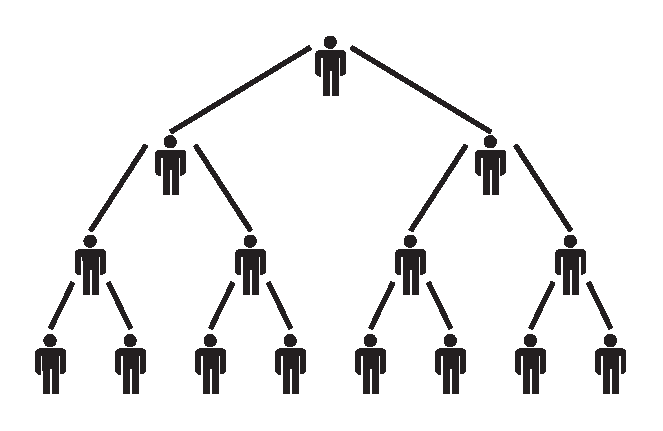
\includegraphics[width=4in]{../../epsimages/ch2sequencesexampleflu.eps}
\caption{Each person infects two more people with the flu virus.}
\label{fig:mp:s:geometricflu}
\end{center}
\end{figure}

Again we can tabulate the events and formulate an equation for the general case:
\begin{center}
\begin{tabular}{|c|l|}\hline
\hline \textbf{Day}, $n$ & \textbf{Number of newly-infected people} \\\hline
\hline 1 & $2 \: \: \: = 2$ \\
\hline 2 & $4 \: \: \: = 2 \times 2 = 2 \times 2^1 $ \\
\hline 3 & $8 \: \: \: = 2 \times 4 = 2 \times 2 \times 2 = 2 \times 2^2$ \\
\hline 4 & $16 \: = 2 \times 8 = 2 \times 2 \times 2 \times 2 = 2 \times 2^3$ \\
\hline 5 & $32 \: = 2 \times 16 = 2 \times 2 \times 2 \times 2 \times 2 = 2 \times 2^4$ \\
\hline \vdots & \qquad \qquad \qquad \qquad \vdots \\
\hline $n$ & $\: \: \quad = 2 \times 2 \times 2 \times 2 \times \ldots \times 2 = 2 \times 2^{n-1}$
\\
\hline\hline
\end{tabular}
\end{center}

The above table represents the number of \textbf{newly-infected} people after $n$ days since you
first infected your $2$ friends. 

You sneeze and the virus is carried over to $2$ people who start the chain ($a_1 = 2$).
The next day, each one then infects $2$ of their friends. Now $4$ people are newly-infected.
Each of them infects $2$ people the third day, and $8$ people are infected, and so on.
These events can be written as a geometric sequence:
\begin{eqnarray*}
2; \: 4; \: 8; \: 16; \: 32; \: \ldots
\end{eqnarray*}

Note the common ratio ($2$) between the events. Recall from the linear arithmetic sequence how the
common difference between terms was established. In the geometric sequence we can determine the
\textit{common ratio}, $r$, from

\begin{equation}
\frac{a_2}{a_1} = \frac{a_3}{a_2} = r
\end{equation}

Or, more generally,
\begin{equation}
\label{eq:mp:s:geomseq:1}
\frac{a_n}{a_{n-1}} = r
\end{equation}

\Activity{}{Common Ratio of Geometric Sequence}{Determine the common ratio for the following
geometric sequences:
\begin{enumerate}
\item{$5;~ 10;~ 20;~40;~ 80; \ldots$}
\item{$\frac{1}{2};~\frac{1}{4};~\frac{1}{8};\ldots$}
\item{$7;~28;~112;~448;\ldots$}
\item{$2;~6;~18;~54;\ldots$}
\item{$-3;~30;~ -300;~ 3000;\ldots$}
\end{enumerate}}
% -----------------------------------------------------------------

\subsection{General Equation for the $n^{th}$-Term of a Geometric Sequence}

From the flu example above we know that $a_1 = 2$ and $r = 2$, and we have seen from the table that the
$n^{th}$-term is given by $a_n = 2 \times 2^{n-1}$. Thus, in general,
\begin{equation}
a_n = a_1 \,.\, r^{n-1}
\end{equation}
where $a_1$ is the first term and $r$ is called the \textit{common ratio}. 

So, if we want to know how many people are newly-infected after 10 days, we need to work
out $a_{10}$:
\begin{eqnarray*}
a_n &=& a_1 \,.\, r^{n-1} \\
a_{10} &=& 2 \times 2^{10-1} \\
&=& 2 \times 2^9 \\
&=& 2 \times 512 \\
&=& 1024
\end{eqnarray*}

That is, after 10 days, there are $1~024$ newly-infected people.

Or, after how many days would $16~384$ people be newly-infected with the flu virus?
\begin{eqnarray*}
a_n &=& a_1 \,.\, r^{n-1} \\
16~384 &=& 2 \times 2^{n-1} \\
16~384 \div 2 &=& 2^{n-1} \\
8~192 &=& 2^{n-1} \\
2^{13} &=& 2^{n-1} \\
13 &=& n - 1 \\
n &=& 14
\end{eqnarray*}

That is, after 14 days $16~384$ people are newly-infected.

\Activity{}{General Equation of Geometric Sequence}{Determine the formula for the $n^{th}$-term of the following geometric
sequences:
\begin{enumerate}
\item{$5;~ 10;~ 20;~ 40;~ 80; \ldots$}
\item{$\frac{1}{2};~\frac{1}{4};~\frac{1}{8};\ldots$}
\item{$7;~28;~ 112;~ 448;\ldots$}
\item{$2, 6, 18, 54,\ldots$}
\item{$-3;~ 30;~ -300;~ 3000;\ldots$}
\end{enumerate}}

%===========================================================

\Exercise{}{
\begin{enumerate}
\item{What is the important characteristic of an arithmetic sequence?}
\item{Write down how you would go about finding the formula for the $n^{\rm{th}}$ term of an arithmetic sequence?}\
\item{A single square is made from $4$ matchsticks. To make two squares in a row takes $7$ matchsticks, while three
squares in a row takes $10$ matchsticks. Determine:
\begin{enumerate}
\item the first term
\item the common difference
\item the formula for the general term
\item how many matchsticks are in a row of $25$ squares
\end{enumerate}
\begin{center}
\begin{pspicture}(0,0)(8,2)
%\psgrid[gridcolor=gray]
\def\match{\psline(0,0)(2,0)\psellipse*(1.8,0)(0.2,0.1)}
\rput(0,0){\match}
\rput{90}(2,0){\match}
\rput{180}(2,2){\match}
\rput{270}(0,2){\match}
\rput(2,0){\rput(0,0){\match}
\rput{90}(2,0){\match}
\rput{180}(2,2){\match}}
\rput(4,0){\rput(0,0){\match}
\rput{90}(2,0){\match}
\rput{180}(2,2){\match}}
\rput(6,0){\rput(0,0){\match}
\rput{90}(2,0){\match}
\rput{180}(2,2){\match}}
\end{pspicture}
\end{center}}
\item{$5;\;x;\;y$ is an arithmetic sequence and $x;\;y;\;81$ is a geometric sequence. All terms in
the sequences are integers. Calculate the values of $x$ and $y$.}

% Automatically inserted shortcodes - number to insert 4
\par \practiceinfo
\par \begin{tabular}[h]{cccccc}
% Question 1
(1.)	01cb	&
% Question 2
(2.)	01cc	&
% Question 3
(3.)	01cd	&
% Question 4
(4.)	01ce	&
\end{tabular}}
% Automatically inserted shortcodes - number inserted 4
\end{enumerate}

\section{Recursive Formulae for Sequences}
%\begin{syllabus}
%\item Correctly interpret recursive formulae: (e.g. $T_{n+1}=T_n+T_{n-1}$).
%\end{syllabus}

When discussing arithmetic and quadratic sequences, we noticed that the difference between two
consecutive terms in the sequence could be written in a general way. 

For an arithmetic sequence, where a new term is calculated by taking the previous term and adding a
constant value, $d$:
\begin{eqnarray*}
a_n = a_{n-1} + d
\end{eqnarray*}
The above equation is an example of a \textit{recursive equation} since we can calculate the
$n^{th}$-term only by considering the previous term in the sequence. Compare this with Equation
(\ref{eq:mp:s:arithseq:2}),
\begin{equation}
a_n = a_1 + d \,.\, (n - 1)
\end{equation}
where one can directly calculate the $n^{th}$-term of an arithmetic sequence without knowing
previous terms. 

For quadratic sequences, we noticed the difference between consecutive terms is given by
(\ref{eq:mp:s:quadseq:2}):
\begin{eqnarray*}
a_n - a_{n-1} = D \,.\, (n-2) + d
\end{eqnarray*}

Therefore, we re-write the equation as
\begin{equation}
a_n = a_{n-1} + D \,.\, (n-2) + d
\end{equation}
which is then a recursive equation for a quadratic sequence with common second difference, $D$. 

Using (\ref{eq:mp:s:geomseq:1}), the recursive equation for a geometric sequence is:
\begin{equation}
a_n = r \,.\, a_{n-1}
\end{equation}
\\
Recursive equations are extremely powerful: you can work out every term in the series just by
knowing previous terms. As you can see from the examples above, working out $a_n$ using the previous
term $a_{n-1}$ can be a much simpler computation than working out $a_n$ from scratch using a general
formula. This means that using a recursive formula when using a computer to work out a sequence
would mean the computer would finish its calculations significantly quicker.

\Activity{}{Recursive Formula}{Write the first five terms of the following sequences, given their
recursive formulae:
\begin{enumerate}
\item{$a_n=2a_{n-1}+3, a_1=1$}
\item{$a_n=a_{n-1}, a_1=11$}
\item{$a_n=2a^2_{n-1}, a_1=2$}
\end{enumerate}}

\Extension{\textbf{The Fibonacci Sequence}}{\\
Consider the following sequence:
\begin{eqnarray}
0; \: 1; \: 1; \: 2; \: 3; \: 5; \: 8; \: 13; \: 21; \: 34; \: \ldots
\end{eqnarray}
\\
The above sequence is called the \textit{Fibonacci sequence}. Each new term is calculated by adding the previous two terms. Hence, we can write down the recursive equation:
\begin{eqnarray}
a_n = a_{n-1} + a_{n-2}
\end{eqnarray}}

\section{Series}
\label{mp:se}
In this section we simply work on the concept of \textit{adding} up the numbers belonging to arithmetic and geometric sequences. We call the sum of \textit{any} sequence of numbers a \textit{series}.

\subsection{Some Basics}
If we add up the terms of a sequence, we obtain what is called a \textit{series}. If we only sum a finite number of terms, we get a \textit{finite series}. We use the symbol $S_n$ to mean the sum of the first $n$ terms of a sequence
$\{a_1; \: a_2; \: a_3; \ldots ; a_n \}$:
\begin{eqnarray}
S_n = a_1 + a_2 + a_3 + \ldots + a_n
\end{eqnarray}

For example, if we have the following sequence of numbers
\begin{eqnarray*}
1; \: 4; \: 9; \: 25; \: 36; \: 49; \: \ldots
\end{eqnarray*}
and we wish to find the sum of the first four terms, then we write
\begin{eqnarray*}
S_4 = 1 + 4 + 9 + 25 = 39
\end{eqnarray*}
The above is an example of a finite series since we are only summing four terms.

If we sum infinitely many terms of a sequence, we get an \textit{infinite series}:
\begin{eqnarray}
S_\infty = a_1 + a_2 + a_3 + \ldots
\end{eqnarray}

\subsection{Sigma Notation}
%\begin{syllabus}
%\item Correctly interpret sigma notation.
%\end{syllabus}

In this section we introduce a notation that will make our lives a little easier.

A sum may be written out using the summation symbol $\sum$\,. This symbol is \textit{sigma}, which is the capital letter ``S'' in the Greek alphabet. It indicates that you must sum the expression to the \textit{right} of it:
\begin{equation}
\label{eq:mp:se:sigma}
\sum_{i=m}^n a_i = a_m + a_{m+1} + \ldots + a_{n-1}+ a_n
\end{equation}
where
\begin{itemize}
\item $i$ is the index of the sum;
\item $m$ is the lower bound (or start index), shown below the summation symbol;
\item $n$ is the upper bound (or end index), shown above the summation symbol;
\item $a_i$ is a term of a sequence.
\end{itemize}

The index $i$ increases from $m$ to $n$ in steps of $1$.

If we are summing from $i=1$ (which implies summing from the first term in a sequence), then we can use either $S_n$- or $\sum$-notation since they mean the same thing:
\begin{equation}
\label{eq:mp:se:Ssigma}
S_n=\sum_{i=1}^n a_i = a_1 + a_2 + \ldots + a_n
\end{equation}

For example, in the following sum,
\begin{equation*}
\sum_{i=1}^5 i
\end{equation*}
we have to add together all the terms in the sequence $a_i=i$ from $i=1$ up until $i=5$:
\begin{equation*}
\sum_{i=1}^5 i = 1 + 2 + 3 + 4 + 5 = 15
\end{equation*}

\subsubsection{Examples}

\begin{enumerate}
\item
\begin{eqnarray*}
\sum_{i=1}^6 2^i &=& 2^1 + 2^2 + 2^3 + 2^4 + 2^5 + 2^6 \\
&=& 2 + 4 + 8 + 16 + 32 + 64 \\
&=& 126
\end{eqnarray*}
\item
\begin{eqnarray*}
\sum_{i=3}^{10} (3x^i) = 3x^3 + 3x^4 + \ldots + 3x^9 + 3x^{10}
\end{eqnarray*}
for any value $x$.
\end{enumerate}

\subsubsection{Some Basic Rules for Sigma Notation}

\begin{enumerate}
\item {Given two sequences, $a_i$ and $b_i$,
\begin{eqnarray}
\label{eq:mp:series:sigma:rule1}
\sum_{i=1}^n (a_i + b_i) &=& \sum_{i=1}^n a_i + \sum_{i=1}^n b_i
\end{eqnarray}
}

\item {For any constant $c$ that is not dependent on the index $i$,
\begin{eqnarray}
\label{eq:mp:series:sigma:rule2}
\sum_{i=1}^n c \,.\, a_i &=& c \,.\, a_1 + c \,.\, a_2 + c \,.\, a_3 + \ldots + c \,.\, a_n \nonumber \\
&=& c \; (a_1 + a_2 + a_3 + \ldots + a_n) \nonumber \\
&=& c \sum_{i=1}^n a_i
\end{eqnarray}
}
\end{enumerate}
\pagebreak
\Exercise{}{
\begin{enumerate}
\item What is $\sum_{k=1}^4 \limits 2$?
\item Determine $\sum_{i=-1}^3 \limits i$.
\item Expand $\sum_{k=0}^5 \limits i$.
\item{Calculate the value of $a$ if:
\nequ{\sum_{k=1}^{3}a\,.\, 2^{k-1}=28}}
\end{enumerate}

% Automatically inserted shortcodes - number to insert 4
\par \practiceinfo
\par \begin{tabular}[h]{cccccc}
% Question 1
(1.)	01cf	&
% Question 2
(2.)	01cg	&
% Question 3
(3.)	01ch	&
% Question 4
(4.)	01ci	&
\end{tabular}}
% Automatically inserted shortcodes - number inserted 4
%\begin{syllabus}
%\item Grade 12
%\item Prove and correctly select the formula for and calculate the sum of series, including:
%\begin{eqnarray*}
%\sum_{i=1}^n 1 &=& n \\
%\sum_{i=1}^n i^2 &=& \frac{n(2n+1)(n+1)}{6} \mbox{ not in syllabus, mark as extra}\\
%\sum_{i=1}^n i &=& \frac{n(n+1)}{2} \\
%\sum_{i=1}^n a+(i-1)d &=& \frac n2 (2a+(n-1))\\
%\sum_{i=1}^n a.r^{i-1} &=& \frac{a(r^n-1)}{r-1}\\
%\sum_{i=1}^\infty a.r^{i-1} &=& \frac a{1-r} \qquad -1<1
%\end{eqnarray*}
%\end{syllabus}

\section{Finite Arithmetic Series}

Remember that an arithmetic sequence is a sequence of numbers, such that the difference between any term and the previous term is a constant number, $d$, called the \textbf{constant difference}:
\begin{eqnarray}
\label{eq:mp:series:lin:gen}
a_n = a_1 + d \; (n - 1)
\end{eqnarray}
where
\begin{itemize}
\item $n$ is the index of the sequence;
\item $a_n$ is the $n^{th}$-term of the sequence;
\item $a_1$ is the first term;
\item $d$ is the common difference.
\end{itemize}

When we sum a finite number of terms in an arithmetic sequence, we get a \textit{finite arithmetic series}.

A simple arithmetic sequence is when $a_1=1$ and $d=0$ in the general form \eqref{eq:mp:series:lin:gen}; in other words all the terms in the sequence are $1$:
\begin{eqnarray*}
a_i &=& a_1 + d \; (i - 1) \\
&=& 1 + 0 \,.\, (i - 1) \\
&=& 1 \\
\{a_i\} &=& \{1; \: 1; \: 1; \: 1; \: 1; \: \ldots \}
\end{eqnarray*}
If we wish to sum this sequence from $i=1$ to any positive integer $n$, we would write
\begin{equation*}
\sum_{i=1}^n {a_i} = \sum_{i=1}^n 1 = 1 + 1 + 1 + \ldots + 1 \qquad (n\textrm{ times})
\end{equation*}

Because all the terms are equal to $1$, it means that if we sum to $n$ we will be adding $n$-number of $1$'s together, which is simply equal to $n$:
\begin{equation}
\boxed{\sum_{i=1}^n 1 = n}
\end{equation}

Another simple arithmetic sequence is when $a_1=1$ and $d=1$, which is the sequence of positive integers:
\begin{eqnarray*}
a_i &=& a_1 + d \; (i - 1) \\
&=& 1 + 1 \,.\, (i - 1) \\
&=& i \\
\{a_i\} &=& \{1; \: 2; \: 3; \: 4; \: 5; \: \ldots \}
\end{eqnarray*}
If we wish to sum this sequence from $i=1$ to any positive integer $n$, we would write
\begin{equation}
\label{eq:mp:se:fa:simple:sum1}
\sum_{i=1}^n i = 1 + 2 + 3 + \ldots + n
\end{equation}
This is an equation with a very important solution as it gives the answer to the sum of positive integers.

\begin{IFact}{Mathematician, Karl Friedrich Gauss, discovered this proof when he was only 8 years old. His teacher had decided to give his class a problem which would distract them for the entire day by asking them to add all the numbers from $1$ to $100$. Young Karl realised how to do this almost instantaneously and shocked the teacher with the correct answer, $5050$.}
\end{IFact}

We first write $S_n$ as a sum of terms in ascending order:
\begin{equation}
\label{eq:mp:series:arith:sum_integers1}
S_n = 1 + 2 + \ldots + (n - 1) + n
\end{equation}
\noindent
We then write the same sum but with the terms in descending order:
\begin{equation}
\label{eq:mp:series:arith:sum_integers2}
S_n = n + (n-1) + \ldots + 2 + 1
\end{equation}
We then add corresponding pairs of terms from Equations \eqref{eq:mp:series:arith:sum_integers1} and \eqref{eq:mp:series:arith:sum_integers2}, and we find that the sum for each pair is the same, $(n+1)$:
\begin{equation}
2 \; S_n = (n+1) + (n+1) + \ldots + (n+1) + (n+1)
\end{equation}
We then have $n$-number of $(n+1)$-terms, and by simplifying we arrive at the final result:
\begin{eqnarray*}
2 \; S_n &=& n \; (n + 1) \\
S_n &=& \frac {n}{2} \; (n + 1)
\end{eqnarray*}
\begin{equation}
\label{eq:mp:series:sum_integers}
\boxed{S_n = \sum_{i=1}^n i = \frac {n}{2} \; (n + 1)}
\end{equation}
Note that this is an example of a quadratic sequence.

\subsection{General Formula for a Finite Arithmetic Series}
If we wish to sum any arithmetic sequence, there is no need to work it out term-for-term. We will now determine the general formula to evaluate a finite arithmetic series. We start with the general formula for an arithmetic sequence and sum it from $i=1$ to any positive integer $n$:
\begin{eqnarray*}
\sum_{i=1}^n a_i &=& \sum_{i=1}^n \; [a_1 + d \, (i-1)] \\
&=& \sum_{i=1}^n \; (a_1 + di - d) \\
&=& \sum_{i=1}^n \; [(a_1 - d) + di] \\
&=& \sum_{i=1}^n \; (a_1 - d) + \sum_{i=1}^n \; (di) \\
&=& \sum_{i=1}^n \; (a_1 - d) + d \; \sum_{i=1}^n \; i \\
&=& (a_1 - d) \, n + \frac {dn}{2} \; (n + 1) \\
&=& \frac{n}{2} \: (2a_1 - 2d + dn + d) \\
&=& \frac{n}{2} \: (2a_1 + dn - d) \\
&=& \frac{n}{2} \: [\, 2a_1 + d \, (n - 1) \,]
\end{eqnarray*}
So, the general formula for determining an arithmetic series is given by
\begin{equation}
\label{eq:mp:se:fa:3}
\boxed {S_n = \sum_{i=1}^n \; [\, a_1 + d \, (i-1) \,] = \frac{n}{2} \: [\, 2a_1 + d \, (n - 1) \,]}
\end{equation}
For example, if we wish to know the series $S_{20}$ for the arithmetic sequence $a_i= 3 + 7 \, (i-1)$, we could either calculate each term individually and sum them:
\begin{eqnarray*}
S_{20} &=& \sum_{i=1}^{20} \; [3 + 7 \, (i-1)] \\
&=& 3 + 10 + 17 + 24 + 31 + 38 + 45 + 52 + \\
&& 59 + 66 + 73 + 80 + 87 + 94 + 101 + \\
&& 108 + 115 + 122 + 129 + 136 \\
&=& 1390
\end{eqnarray*}
or, more sensibly, we could use Equation \eqref{eq:mp:se:fa:3} noting that $a_1=3$, $d=7$ and $n=20$ so that
\begin{eqnarray*}
\label{eq:mp:se:fa:ex:smartway}
S_{20} &=& \sum_{i=1}^{20} \; [3 + 7 \, (i-1)] \\
&=& \textstyle \small {\frac{20}{2}} \: [2 \,.\, 3 + 7 \, (20 - 1) ] \\
&=& 1390
\end{eqnarray*}
This example demonstrates how useful Equation \eqref{eq:mp:se:fa:3} is.

\Exercise{}{
\begin{enumerate}

\item The sum to $n$ terms of an arithmetic series is $S_n = \dfrac{n}{2} \, (7n + 15)$.
\begin{enumerate}
\item{How many terms of the series must be added to give a sum of $425$?}
\item{Determine the $6^{th}$ term of the series.}
\end{enumerate}

\item The sum of an arithmetic series is $100$ times its first term, while the last term is $9$ times the first term. Calculate the number of terms in the series if the first term is not equal to zero.

\item The common difference of an arithmetic series is $3$. Calculate the value of $n$ for which the $n^{th}$ term of the series is $93$, and the sum of the first $n$ terms is $975$.

\item The sum of $n$ terms of an arithmetic series is $5n^2 - 11n$ for all values of $n$. Determine the common difference.

\item{The third term of an arithmetic sequence is $-7$ and the $7^{th}$ term is $9$. Determine the sum of the first $51$ terms of the sequence.}

\item{Calculate the sum of the arithmetic series $4+7+10+\cdots+901$.}
\end{enumerate}

% Automatically inserted shortcodes - number to insert 6
\par \practiceinfo
\par \begin{tabular}[h]{cccccc}
% Question 1
(1.)	01cj	&
% Question 2
(2.)	01ck	&
% Question 3
(3.)	01cm	&
% Question 4
(4.)	01cn	&
% Question 5
(5.)	01cp	&
% Question 6
(6.)	01cq	\\ % End row of shortcodes
\end{tabular}}
% Automatically inserted shortcodes - number inserted 6
\section{Finite Squared Series}
When we sum a finite number of terms in a quadratic sequence, we get a \textit{finite
quadratic series}. The general form of a quadratic series is quite complicated,
so we will only look at the simple case when $D=2$ and $d=(a_2 - a_1)=3$, where $D$ is the common second difference and $d$ is the first difference. This is the sequence of squares of the integers:
\begin{eqnarray*}
\label{eq:mp:se:quad:seq}
a_i &=& i^{\,2} \\
\{a_i\} &=& \{1^2; \: 2^2; \: 3^2; \: 4^2; \: 5^2; \: 6^2; \: \ldots \} \\
&=& \{1; \: 4; \: 9; \: 16; \: 25; \: 36; \: \ldots \}
\end{eqnarray*}
If we wish to sum this sequence and create a series, we write
\begin{equation*}
\label{eq:mp:se:fs:sum}
S_n=\sum_{i=1}^n i^{\,2} = 1 + 4 + 9 + \ldots + n^2
\end{equation*}
which can be written, in general, as
\begin{equation}
\label{eq:mp:se:fs:2}
\boxed{S_n = \sum_{i=1}^n i^2 = \frac{n}{6}(2n + 1)(n + 1)}
\end{equation}
\\
The proof for Equation \eqref{eq:mp:se:fs:2} can be found under the \textit{Extension} block that follows:
\\
\Extension{Derivation of the Finite Squared Series}{
We will now prove the formula for the finite squared series:
\begin{equation*}
S_n=\sum_{i=1}^n i^{\,2} = 1 + 4 + 9 + \ldots + n^2
\end{equation*}
We start off with the expansion of ${(k + 1)}^3$.
\begin{eqnarray*}
{(k + 1)}^3 &=& k^3 + 3k^2 + 3k + 1 \\
{(k + 1)}^3 - k^3 &=& 3k^2 + 3k + 1
\end{eqnarray*}
\begin{eqnarray*}
k=1 &:& \quad 2^3 - 1^3 = 3(1)^2 + 3(1) + 1 \\
\vspace{6pt} \\
k=2 &:& \quad 3^3 - 2^3 = 3(2)^2 + 3(2) + 1 \\
\vspace{6pt} \\
k=3 &:& \quad 4^3 - 3^3 = 3(3)^2 + 3(3) + 1 \\
&\vdots& \\
k=n &:& \quad {(n + 1)}^3 - n^3 = 3n^2 + 3n + 1
\end{eqnarray*}
If we add all the terms on the right and left, we arrive at
\begin{eqnarray*}
{(n + 1)}^3 - 1 &=& \sum_{i=1}^n \: (3i^2 + 3i + 1) \\
\vspace{12pt} \\
n^3 + 3n^2 + 3n + 1 - 1 &=& 3\,\sum_{i=1}^n \: i^2 + 3\,\sum_{i=1}^n \: i + \sum_{i=1}^n \: 1 \\
\vspace{12pt} \\
n^3 + 3n^2 + 3n &=& 3\,\sum_{i=1}^n \: i^2 + \frac{3n}{2}\,(n + 1) + n \\
\vspace{12pt} \\
\sum_{i=1}^n \: i^2 &=& \frac{1}{3}\,[n^3 + 3n^2 + 3n - \frac{3n}{2}\,(n + 1) - n] \\
\vspace{12pt} \\
&=& \frac{1}{3}\,(n^3 + 3n^2 + 3n - \frac{3}{2}\,n^2 - \frac{3}{2}\,n - n) \\
\vspace{12pt} \\
&=& \frac{1}{3}\,(n^3 + \frac{3}{2}\,n^2 + \frac{1}{2}\,n) \\
\vspace{12pt} \\
&=& \frac{n}{6}\,(2n^2 + 3n + 1)
\end{eqnarray*}
Therefore,
\begin{equation*}
\boxed{\sum_{i=1}^n \: i^2 = \frac{n}{6}(2n + 1)(n + 1)}
\end{equation*}}


\section{Finite Geometric Series}
When we sum a known number of terms in a geometric sequence, we get a \textit{finite geometric series}. %We know from \eqref{eq:mp:s:geom:genalt}, that 
We can write out each term of a geometric sequence in the general form:
\begin{equation}
a_n = a_1 \,.\, r^{n-1}
\end{equation}
where
\begin{itemize}
\item $n$ is the index of the sequence;
\item $a_n$ is the $n^{th}$-term of the sequence;
\item $a_1$ is the first term;
\item $r$ is the common ratio (the ratio of any term to the previous term).
\end{itemize}

\vspace{12pt}
By simply adding together the first $n$ terms, we are actually writing out the series
\begin{equation}
\label{eq:mp:s:geom:S}
S_n = a_1 + a_1\,r + a_1\,r^2 + \ldots + a_1\,r^{n-2} + a_1\,r^{n-1}
\end{equation}
We may multiply the above equation by $r$ on both sides, giving us
\begin{equation}
\label{eq:mp:s:geom:rS}
rS_n = a_1\,r + a_1\,r^2 + a_1\,r^3 + \ldots + a_1\,r^{n-1} + a_1\,r^n
\end{equation}
You may notice that all the terms on the right side of \eqref{eq:mp:s:geom:S} and \eqref{eq:mp:s:geom:rS} are the same, except the first and last terms. If we subtract \eqref{eq:mp:s:geom:S} from \eqref{eq:mp:s:geom:rS}, we are left with just
\begin{eqnarray*}
\label{eq:mp:s:geom:proof}
rS_n - S_n = a_1\,r^n - a_1 \\
S_n(r - 1) = a_1\,(r^n - 1)
\end{eqnarray*}
Dividing by $(r-1)$ on both sides, we arrive at the general form of a geometric series:
\begin{equation}
\label{eq:mp:se:fg:4}
\boxed{S_n = \sum_{i=1}^n a_1 \,.\, r^{i-1} = \frac{a_1 \, (r^n - 1)}{r-1}}
\end{equation}
% The following video summarises what you have learnt so far about sequences and series:
% Khan Academy video on sequences and series, part 1:SIYAVULA-VIDEO:http://cnx.org/content/m39301/latest/#series-1
\mindsetvid{Khan on sequences}{VMgjq}
\Exercise{}{
\begin{enumerate}
\item Prove that $$a + ar + ar^2 + ... + ar^{n-1} = \dfrac{a\,(1 - r^n)}{(1-r)}$$
\item{Given the geometric sequence $1;\;-3;\; 9;\;\dots$ determine:
\begin{enumerate}
\item{The $8^{\rm{th}}$ term of the sequence}
\item{The sum of the first eight terms of the sequence.}
\end{enumerate}}
\item{Determine:
\nequ{\sum_{n=1}^{4}3\,.\,2^{n-1}}}
\item Find the sum of the first $11$ terms of the geometric series $6 + 3 + \tfrac{3}{2} + \tfrac{3}{4} + \ldots$
\item Show that the sum of the first $n$ terms of the geometric series $$54 + 18 + 6 + ... + 5 \, (\tfrac{1}{3})^{n-1}$$ is given by $81 - 3^{4-n}$.
\item The eighth term of a geometric sequence is $640$. The third term is $20$. Find the sum of the first 7 terms.
\item Solve for $n$: $\sum_{t=1}^n \limits 8 \, (\tfrac{1}{2})^t = 15\tfrac{3}{4}$.
\item The ratio between the sum of the first three terms of a geometric series and the sum of the $4^{th}$-, $5^{th}$- and $6^{th}$-terms of the same series is $8:27$. Determine the common ratio and the first 2 terms if the third term is $8$.

% Automatically inserted shortcodes - number to insert 8
\par \practiceinfo
\par \begin{tabular}[h]{cccccc}
% Question 1
(1.)	01cr	&
% Question 2
(2.)	01cs	&
% Question 3
(3.)	01ct	&
% Question 4
(4.)	01cu	&
% Question 5
(5.)	01cv	&
% Question 6
(6.)	01cw	\\ % End row of shortcodes
% Question 7
(7.)	01cx	&
% Question 8
(8.)	01cy	&
\end{tabular}}
% Automatically inserted shortcodes - number inserted 8

\end{enumerate}

\section{Infinite Series}
Thus far we have been working only with finite sums, meaning that whenever we determined the sum of a series, we only considered the sum of the first $n$ terms. In this section, we consider what happens when we add infinitely many terms together. You might think that this is a silly question - surely the answer will be $\infty$ when one sums infinitely many numbers, no matter how small they are? The surprising answer is that while in some cases one will reach $\infty$ (like when you try to add all the positive integers together), there are some cases in which one will get a finite answer. If you don't believe this, try doing the following sum, a geometric series, on your calculator or computer:
$$\tfrac{1}{2} + \tfrac{1}{4} + \tfrac{1}{8} + \tfrac{1}{16} + \tfrac{1}{32} + \ldots $$
You might think that if you keep adding more and more terms you will eventually get larger and larger numbers, but in fact you won't even get past $1$ - try it and see for yourself!

We denote the sum of an infinite number of terms of a sequence by
\begin{eqnarray*}
S_\infty = \sum^\infty_{i=1} a_i
\end{eqnarray*}

When we sum the terms of a series, and the answer we get after each summation gets closer and closer to some number, we say that the series \textit{converges}. If a series does not converge, then we say that it \textit{diverges}.

\subsection{Infinite Geometric Series}

There is a simple test for knowing instantly which geometric series converges and which diverges. When $r$, the common ratio, is strictly between $-1$ and $1$, i.e. $-1 < r < 1$, the infinite series will converge, otherwise it will diverge. There is also a formula for working out the value to which the series converges.

Let's start off with Formula \eqref{eq:mp:se:fg:4} for the finite geometric series:
\begin{equation*}
S_n = \sum_{i=1}^n a_1 \,.\, r^{i-1} = \frac{a_1 \, (r^n - 1)}{r-1}
\end{equation*}

Now we will investigate the behaviour of $r^n$ for $-1<r<1$ as $n$ becomes larger.

Take $r=\frac{1}{2}$:
\begin{eqnarray*}
n=1 &:& r^n = r^1 =(\tfrac{1}{2})^1 = \tfrac{1}{2} \\
n=2 &:& r^n = r^2 =(\tfrac{1}{2})^2 = \tfrac{1}{2} \,.\, \tfrac{1}{2} = \tfrac{1}{4} < \tfrac{1}{2} \\
n=3 &:& r^n = r^3 =(\tfrac{1}{2})^3 = \tfrac{1}{2} \,.\, \tfrac{1}{2} \,.\, \tfrac{1}{2} = \tfrac{1}{8} < \tfrac{1}{4}
\end{eqnarray*}

Since $r$ is in the range $-1<r<1$, we see that $r^n$ gets closer to $0$ as $n$ gets larger.

Therefore,
\begin{eqnarray*}
S_n &=& \frac{a_1 \, (r^n - 1)}{r - 1} \\
\vspace{12pt} \\
S_\infty &=& \frac{a_1 \, (0 - 1)}{r - 1} \qquad \mathrm{ for } -1 < r < 1 \\
\vspace{12pt} \\
&=& \frac {-a_1}{r - 1} \\
\vspace{12pt} \\
&=& \frac {a_1}{1 - r}
\end{eqnarray*}

The sum of an infinite geometric series is given by the formula
\begin{eqnarray}
\label{eq:mp:se:ig:4}
\boxed{S_\infty = \sum_{i=1}^\infty a_1r^{i-1} = \frac {a_1}{1-r} \qquad \mathrm{ for } \qquad -1<r<1 }
\end{eqnarray}
where $a_1$ is the first term of the series and $r$ is the common ratio.
% Khan Academy video on sequences and series, part 2:SIYAVULA-VIDEO:http://cnx.org/content/m39301/latest/#series-2

\mindsetvid{Khan on sequences 2}{VMgly}

\Exercise{}{
\begin{enumerate}
\item What does $(\tfrac{2}{5})^n$ approach as $n$ tends towards $\infty$?
\item{Given the geometric series:
\nequ{2\,.\,(5)^5+2\,.\,(5)^4+2\,.\,(5)^3+\ldots}
\begin{enumerate}
\item Show that the series converges
\item Calculate the sum to infinity of the series
\item Calculate the sum of the first eight terms of the series, correct to two decimal places.
\item Determine
\nequ{\sum_{n=9}^{\infty}2\,.\,{5}^{6-n}}
correct to two decimal places using previously calculated results.
\end{enumerate}}
\item Find the sum to infinity of the geometric series $3 + 1 + \tfrac{1}{3} + \tfrac{1}{9} + \ldots$
\item Determine for which values of $x$, the geometric series $$2 + \tfrac{2}{3} \, (x+1) +\tfrac{2}{9} \, (x+1)^2 + \ldots$$ will converge.
\item The sum to infinity of a geometric series with positive terms is $4\tfrac{1}{6}$ and the sum of the first two terms is $2\tfrac{2}{3}$. Find $a$, the first term, and $r$, the common ratio between consecutive terms.
\end{enumerate}

% Automatically inserted shortcodes - number to insert 5
\par \practiceinfo
\par \begin{tabular}[h]{cccccc}
% Question 1
(1.)	01cz	&
% Question 2
(2.)	01d0	&
% Question 3
(3.)	01d1	&
% Question 4
(4.)	01d2	&
% Question 5
(5.)	01d3	&
\end{tabular}}
% Automatically inserted shortcodes - number inserted 5
<<<<<<< HEAD
\pagebreak
=======

>>>>>>> 87fbe17a7d2a59e192d41390edbc6425615b0e12
\begin{eocexercises}{}
\begin{enumerate}

\item Is $1 + 2 + 3 + 4 + ...$ an example of a \textit{finite series} or an \textit{infinite series}?

\item Calculate $$\sum_{k=2}^6 3 \, {(\tfrac{1}{3})}^{k+2}$$

\item If $x+1$; $x-1$; $2x-5$ are the first three terms of a convergent geometric series, calculate the:
\begin{enumerate}
\item Value of $x$.
\item Sum to infinity of the series.
\end{enumerate}

\item Write the sum of the first twenty terms of the series $6 + 3 + \tfrac{3}{2} + \tfrac{3}{4} + ...$ in $\sum$\,-notation.

\item For the geometric series, $$54 + 18 + 6 + ... + 5 \, (\tfrac{1}{3})^{n-1}$$ calculate the smallest value of $n$ for which the sum of the first $n$ terms is greater than $80.99$.

\item Determine the value of $\sum_{k=1}^\infty \limits 12(\tfrac{1}{5})^{k-1} $.

\item A new soccer competition requires each of $8$ teams to play every other team once.
\begin{enumerate}
\item Calculate the total number of matches to be played in the competition.
\item If each of $n$ teams played each other once, determine a formula for the total number of matches in terms of $n$.
\end{enumerate}

\item The midpoints of the opposite sides of square of length $4$ units are joined to form $4$ new smaller squares. This midpoints of the new smaller squares are then joined in the same way to make even smaller squares. This process is repeated indefinitely. Calculate the sum of the areas of all the squares so formed.

\item Thembi worked part-time to buy a Mathematics book which cost R$29,50$. On 1 February she saved R$1,60$, and everyday saves $30$ cents more than she saved the previous day. (So, on the second day, she saved R$1,90$, and so on.) After how many days did she have enough money to buy the book?

\item Consider the geometric series: $$5 + 2\tfrac{1}{2} + 1\tfrac{1}{4} + \ldots $$
\begin{enumerate}
\item If $A$ is the sum to infinity and $B$ is the sum of the first $n$ terms, write down the value of:
\begin{enumerate}
\item $A$
\item $B$ in terms of $n$.
\end{enumerate}

\item For which values of $n$ is $(A - B) < \tfrac{1}{24}$?
\end{enumerate}

\item A certain plant reaches a height of $118$ mm after one year under ideal conditions in a greenhouse. During the next year, the height increases by $12$ mm. In each successive year, the height increases by $\tfrac{5}{8}$ of the previous year's growth. Show that the plant will never reach a height of more than $150$ mm.

\item Calculate the value of $n$ if $\sum_{a=1}^n \limits \, (20 - 4a) = -20$.

\item Michael saved R$400$ during the first month of his working life. In each subsequent month, he saved $10\%$ more than what he had saved in the previous month.
\begin{enumerate}
\item How much did he save in the $7^{th}$ working month?
\item How much did he save all together in his first 12 working months?
\item In which month of his working life did he save more than R$1~500$ for the first time?
\end{enumerate}

\item A man was injured in an accident at work. He receives a disability grant of R$4~800$ in the first year. This grant increases with a fixed amount each year.
\begin{enumerate}
\item What is the annual increase if, over 20 years, he would have received a total of R$143~500$?
\item His initial annual expenditure is R$2~600$ and increases at a rate of R$400$ per year. After how many years does his expenses exceed his income?
\end{enumerate}
\item{The Cape Town High School wants to build a school hall and is busy with fundraising. Mr. Manuel, an ex-learner of the school and a successful politician, offers to donate money to the school. Having enjoyed mathematics at school, he decides to donate an amount of money on the following basis.
He sets a mathematical quiz with $20$ questions. For the correct answer to the first question (any learner may answer), the school will receive $1$ cent, for a correct answer to the second question, the school will receive $2$ cents, and so on. The donations $1; 2; 4; \ldots$ form a geometric sequence. Calculate (Give your answer to the nearest Rand)
\begin{enumerate}
\item{The amount of money that the school will receive for the correct answer to the $20^{\rm{th}}$ question.}
\item{The total amount of money that the school will receive if all $20$ questions are answered correctly.}
\end{enumerate}
}\item{ The common difference of an arithmetic series is $3$. Calculate the values of $n$ for which the $n^{\rm{th}}$ term of the series is $93$ and the sum of the first $n$ terms is $975$.}

\item{The first term of a geometric sequence is $9$, and the ratio of the sum of the first eight terms to the sum of the first four terms is $97:81$. Find the first three terms of the sequence, if it is given that all the terms are positive.}

\item{$(k-4); \; (k+1); \; m; \; 5k$ is a set of numbers, the first three of which form an arithmetic sequence, and the last three a geometric sequence. Find $k$ and $m$ if both are positive.}

\item{Given: The sequence $6+p \;\!; \; 10+p\;\!; \; 15+p \;$ is geometric.}
\begin{enumerate}
\item{Determine $p$.}
\item{Show that the common ratio is $\tfrac{5}{4}$.}
\item{Determine the $10^{th}$ term of this sequence correct to one decimal place.}
\end{enumerate}

\item{The second and fourth terms of a convergent geometric series are $36$ and $16$, respectively. Find the sum to infinity of this series, if all its terms are positive.}

\item{Evaluate: $\sum_{k=2}^5 \limits \dfrac{k(k+1)}{2}$}

\item{$S_n = 4n^2 + 1$ represents the sum of the first $n$ terms of a particular series. Find the second term.}

\item{Find $p$ if: \qquad $\sum_{k=1}^{\infty} \limits \; 27p^{ k} = \sum_{t=1}^{12} \limits \; (24-3t)$}

\item{Find the integer that is the closest approximation to:$$\dfrac{10^{ 2001} \:+\: 10^{ 2003}}{10^{ 2002} \:+\: 10^{ 2002}}$$}

% \item{Find the pattern and hence calculate: $$1-2+3-4+5-6 \ldots +677 - 678 + \ldots -1000$$}

\item{In each case (substituting the values of $x$ below), determine if the series $\sum_{p=1}^{\infty} \limits (x+2)^p$ converges. If it does, work out what it converges to:}\begin{enumerate}
\item{$x=-\dfrac{5}{2}$}
\item{$x=-5$}
\end{enumerate}

\item{Calculate: \qquad $\sum_{i=1}^{\infty} \limits \; 5 \,.\, 4^{-i}$}

\item{The sum of the first $p$ terms of a sequence is $p \; (p+1)$. Find the $10^{th}$ term.}

\item{The powers of $2$ are removed from the set of positive integers $$1; \: 2; \: 3; \: 4; \: 5; \: 6; \ldots; 1998; \: 1999; \: 2000$$ Find the sum of remaining integers.}

\item{Observe the pattern below:

\begin{pspicture}(-3, -6)(6, 6)
%\psgrid[gridlabels=10pt,gridlabelcolor=black]
%\psaxes[labels=none, ticks=all]{<->}(0, 0)(-4.5, -2.5)(5,3.5)
\psline(6, 6)(0, 0)(6, -6)
\uput[0](1, 0){A}
\multido{\n=-1+1}{3}{\uput[0](2, \n){B}}
\multido{\n=-2+1}{5}{\uput[0](3, \n){C}}
\multido{\n=-3+1}{7}{\uput[0](4, \n){D}}
\multido{\n=-4+1}{9}{\uput[0](5, \n){E}}
\end{pspicture}

\begin{enumerate}
\item{If the pattern continues, find the number of letters in the column containing M's.}
\item{If the total number of letters in the pattern is $361$, which letter will be in the last column.}
\end{enumerate}}

\item{The following question was asked in a test:
\begin{quote}
Find the value of $2^{2005} + 2^{2005}$.
\end{quote}
Here are some of the students' answers:\\
\begin{enumerate}
\item Megan said the answer is $4^{2005}$.
\item Stefan wrote down $2^{4010}$.
\item Nina thinks it is $2^{2006}$.
\item Annatte gave the answer $2^{2005 \times 2005}$.
\end{enumerate}
Who is correct? (``None of them" is also a possibility.)}

\item{A shrub of height $110$ cm is planted. At the end of the first year, the shrub is $120$ cm tall. Thereafter, the growth of the shrub each year is half of its growth in the previous year. Show that the height of the shrub will never exceed $130$ cm.}

\end{enumerate}



% CHILD SECTION END 



% CHILD SECTION START 
% Automatically inserted shortcodes - number to insert 31
\par \practiceinfo
\par \begin{tabular}[h]{cccccc}
% Question 1
(1.)	01d4	&
% Question 2
(2.)	01d5	&
% Question 3
(3.)	01d6	&
% Question 4
(4.)	01d7	&
% Question 5
(5.)	01d8	&
% Question 6
(6.)	01d9	\\ % End row of shortcodes
% Question 7
(7.)	01da	&
% Question 8
(8.)	01db	&
% Question 9
(9.)	01dc	&
% Question 10
(10.)	01dd	&
% Question 11
(11.)	01de	&
% Question 12
(12.)	01df	\\ % End row of shortcodes
% Question 13
(13.)	01dg	&
% Question 14
(14.)	01dh	&
% Question 15
(15.)	01di	&
% Question 16
(16.)	01dj	&
% Question 17
(17.)	01dk	&
% Question 18
(18.)	01dm	\\ % End row of shortcodes
% Question 19
(19.)	01dn	&
% Question 20
(20.)	01dp	&
% Question 21
(21.)	01dq	&
% Question 22
(22.)	01dr	&
% Question 23
(23.)	01ds	&
% Question 24
(24.)	01dt	\\ % End row of shortcodes
% Question 25
(25.)	01du	&
% Question 26
(26.)	01dv	&
% Question 27
(27.)	01dw	&
% Question 28
(28.)	01dx	&
% Question 29
(29.)	01dy	&
% Question 30
(30.)	01dz	\\ % End row of shortcodes
% Question 31
(31.)	01e0	&
\end{tabular}
% Automatically inserted shortcodes - number inserted 31
\end{eocexercises}

 \chapter{Finance}
\label{m:f12}

\section{Introduction}
In earlier grades simple interest and compound interest were studied, together with the concept of depreciation. Nominal and effective interest rates were also described. Since this chapter expands on earlier work, it would be best if you revised the work done in Grades 10 and 11.%Chapters~\ref{m:f10} and \ref{m:f11}.

When you master the techniques in this chapter, you will be able to
assess critically how to invest your money when you start working and
earning. And when you are looking at applying for a bond from a bank
to buy a home, you will confidently be able to get out the calculator
and work out how much you could actually save by making additional
repayments. This chapter will provide you with the fundamental
concepts you will need to manage your finances.

\chapterstartvideo{VMgmf}
\section{Finding the Length of the Investment or Loan}
\label{sec:m:f12:term}

%\begin{syllabus}
%\item Calculate the value of $n$ in the formula $A = P(1 + i)^n$
%\end{syllabus}

In Grade 11, we used the Compound Interest formula $A = P(1 + i)^n$ to determine the term of the investment or loan, by trial and error. Remember that $P$ is the initial amount, $A$ is the current amount, $i$ is the interest rate and $n$ is the number of time units (number of months or years). So if we invest an amount and know what the interest rate is, then we can work out how long it will take for the money to grow to the required amount.

Now that you have learnt about logarithms, you are ready to work out the proper algebraic solution. If you need to remind yourself how logarithms work, go to Chapter~\ref{m:f12:logarithms} (on Page~\pageref{m:f12:logarithms}).

The basic finance equation is:
\begin{equation*}
A = P \,.\, (1+i)^n
\end{equation*}

If you don't know what $A$, $P$, $i$ and $n$ represent, then you should definitely revise the work from Grade 10 and 11.

Solving for $n$:
\begin{eqnarray*}
A &=& P(1+i)^n\\
(1+i)^n &=& (A/P)\\
\log((1+i)^n)&=&\log(A/P)\\
n\log(1+i)&=&\log(A/P)\\
n &=& \log(A/P) / \log(1+i)
\end{eqnarray*}

Remember, you do not have to memorise this formula. It is very easy to derive any time you need it. It is simply a matter of writing down what you have, deciding what you need, and solving for that variable.

\begin{wex}{Term of Investment - Logarithms}{Suppose we invested R$3~500$ into a savings account which pays $7,5\%$ compound interest. After an unknown period of time our account is worth R$4~044,69$. For how long did we invest the money? How does this compare with the trial and error answer from Chapters~\ref{m:f11}.}{
\westep{Determine what is given and what is required}
\begin{itemize}
\item{$P$=R$3~500$}
\item{$i$=$7,5$\%}
\item{$A$=R$4~044,69$}
\end{itemize}
We are required to find $n$.
\westep{Determine how to approach the problem}
We know that:
\begin{eqnarray*}
A &=& P(1+i)^n\\
(1+i)^n &=& (A/P)\\
\log((1+i)^n)&=&\log(A/P)\\
n\log(1+i)&=&\log(A/P)\\
n &=& \log(A/P) / \log(1+i)
\end{eqnarray*}

\westep{Solve the problem}
\begin{eqnarray*}
n &=& \log(A/P) / \log(1+i)\\
&=&\frac{\log(\frac{4~044,69}{3~500})}{\log(1+0.075)}\qquad \mbox{Remember that: }7.5\%=\frac{7.5}{100}=0.075\\
&=&2.0
\end{eqnarray*}
\westep{Write final answer}
The R$3~500$ was invested for 2 years.}
\end{wex}

\section{Series of Payments}
%\begin{syllabus}
%\item Apply knowledge of geometric series to solving annuity, bond repayment and sinking fund problems, with or without the use of the formulae:
%\begin{eqnarray*}
%F = \frac{x[(1+i)^n -1]}{i}\\
%P = \frac{x[1- (1+i)^{-n}]}{i}
%\end{eqnarray*}
%\end{syllabus}

By this stage, you know how to do calculations such as `If I want R$1~000$ in three years' time, how much do I need to invest now at $10\%$?'

What if we extend this as follows: ``If I want to draw R$1~000$ next year, R$1~000$ the next year and R$1~000$ after three years, how much do I need to initially put into a bank account earning $10\%$ p.a.\@{} to be able to afford to be able to do this?''

The obvious way of working that out is to work out how much you need now to afford the payments individually and sum them. We'll work out how much is needed now to afford the payment of R$1~000$ in a year $(= $ {R}$1~000\times (1,10)^{-1} = ${R}$909,09)$, the amount needed now for the following year's R$1~000 (= ${R}$1~000\times (1,10)^{-2} = $ {R}$826,45)$ and the amount needed now for the R$1~000$ after three years $(= ${R}$1~000\times (1,10)^{-3} =${R}$751,31)$. Adding these together gives you the amount needed to afford all three payments and you get R$2~486,85$.

So, if you put R$2~486,85$ into a $10\%$ bank account now, you will be able to draw out R$1~000$ in a year, R$1~000$ a year after that, and R$1~000$ a year after that - and your bank account balance will decrease to R$0$. You would have had exactly the right amount of money to do that (obviously!).

You can check this as follows:

\begin{tabular}{lll}
Amount at Time 0 (i.e.\@{} Now) &&= R$2~486,85$\\
Amount at Time 1 (i.e.\@{} a year later) &= R$2~486,85(1+10\%)$ &= R$2~735,54$\\
Amount after withdrawing R$1~000$ &= R$2~735,54 ~-$ R$1~000$ &= R$1~735,54$\\
Amount at Time 2 (i.e.\@{} a year later) &= R$1~735,54(1+10\%)$ &= R$1~909,09$\\
Amount after withdrawing R$1~00$0 &= R$1~909,09 ~-$ R$1~000$ &= R$909,09$\\
Amount at Time 3 (i.e.\@{} a year later) &= R$909,09(1+10\%)$ &= R$1~000$\\
Amount after withdrawing R$1~000$ &= R$1~000 ~-$ R$1~000$ &= R$0$\\
\end{tabular}

Perfect! Of course, for only three years, that was not too bad. But what if I asked you how much you needed to put into a bank account now, to be able to afford R$100$ a month for the next 15 years. If you used the above approach you would still get the right answer, but it would take you weeks!

There is - I'm sure you guessed - an easier way! This section will focus on describing how to work with:
\begin{itemize}
\item{\textbf{annuities} - a fixed sum payable each year or each month, either to provide a pre-determined sum at the end of a number of years or months (referred to as a future value annuity) or a fixed amount paid each year or each month to repay (amortise) a loan (referred to as a present value annuity).}
\item{\textbf{bond repayments} - a fixed sum payable at regular intervals to pay off a loan. This is an example of a present value annuity.}
\item{\textbf{sinking funds} - an accounting term for cash set aside for a particular purpose and invested so that the correct amount of money will be available when it is needed. This is an example of a future value annuity.}
\end{itemize}

\subsection{Sequences and Series}
\label{m:f:ss}
Before we progress, you need to go back and read Chapter~\ref{mp:s} (from Page~\pageref{mp:s}) to revise sequences and series.

In summary, if you have a series of $n$ terms in total which looks like this:
\begin{equation*}
a + ar + ar^2 + \cdots + ar^{n-1} = a [ 1 + r + r^2 + \cdots r^{n-1} ]
\end{equation*}

this can be simplified as:
\begin{eqnarray*}
\frac{a (r^n - 1)}{r-1} &\mbox{useful when $r>1$}\\
\frac{a (1 - r^n)}{1-r} &\mbox{useful when $0\le r <1$}
\end{eqnarray*}

\subsection{Present Values of a Series of Payments}\label{presentvalues}
So having reviewed the mathematics of sequences and series, you might be wondering how this is meant to have any practical purpose! Given that we are in the finance section, you would be right to guess that there must be some financial use to all this. Here is an example which happens in many people's lives - so you know you are learning something practical.

Let us say you would like to buy a property for R$300~000$, so you go to the bank to apply for a mortgage bond. The bank wants it to be repaid by annually payments for the next 20 years, starting at end of this year. They will charge you $15\%$ interest per annum. At the end of the 20 years the bank would have received back the total amount you borrowed together with all the interest they have earned from lending you the money. You would obviously want to work out what the annual repayment is going to be!

Let $X$ be the annual repayment, $i$ is the interest rate, and $M$ is the amount of the mortgage bond you will be taking out.

Time lines are particularly useful tools for visualising the series of payments for calculations, and we can represent these payments on a time line as:

\begin{figure}[htbp]
\begin{center}
\begin{pspicture}(0,0)(10,3)
\psline(0,1.5)(4,1.5) %solid horizontal line
\psline(6,1.5)(10,1.5) %solid horizontal line
\psline[linestyle=dashed](4,1.5)(6,1.5) %dashed horizontal line

\psline[arrows=->](0,1.25)(0,1.75) %arrow at 0
\psline[arrows=->](1,1.25)(1,1.75) %arrow at 1
\psline[arrows=->](2,1.25)(2,1.75) %arrow at 2
\psline[arrows=->](8,1.25)(8,1.75) %arrow at 8
\psline[arrows=->](9,1.25)(9,1.75) %arrow at 9
\psline[arrows=->](10,1.25)(10,1.75) %arrow at 10

\psline(3,1.4)(3,1.6) %vertical line at 3
\psline(7,1.4)(7,1.6) %vertical line at 7

\uput[d](0,1.25){$0$}
\uput[d](1,1.25){$1$}
\uput[d](2,1.25){$2$}
\uput[d](8,1.25){$18$}
\uput[d](9,1.25){$19$}
\uput[d](10,1.25){$20$}

\uput[u](1,1.75){$X$}
\uput[u](2,1.75){$X$}
\uput[u](8,1.75){$X$}
\uput[u](9,1.75){$X$}
\uput[u](10,1.75){$X$}

\uput[r](10.5,1.75){Cash Flows}
\uput[r](10.5,1.25){Time}
\end{pspicture}
\caption{Time line for an annuity (in arrears) of $X$ for $n$ periods.}
\end{center}
\end{figure}

The present value of all the payments (which includes interest) must equate to the (present) value of the mortgage loan amount.

Mathematically, you can write this as:
\begin{equation*}
M = X(1+i)^{-1} + X(1+i)^{-2} + X(1+i)^{-3} + \cdots + X(1+i)^{-20}
\end{equation*}

The painful way of solving this problem would be to do the calculation for each of the terms above - which is $20$ different calculations. Not only would you probably get bored along the way, but you are also likely to make a mistake.

Naturally, there is a simpler way of doing this! You can rewrite the above equation as follows:

\begin{eqnarray*}
M = X[v^1 + v^2 + v^3 + \cdots + v^{20}]\\
\mbox{where $v = (1+i)^{-1} = 1/(1+i)$}
\end{eqnarray*}

Of course, you do not have to use the method of substitution to solve this. We just find this a useful method because you can get rid of the negative exponents - which can be quite confusing! As an exercise - to show you are a real financial whizz - try to solve this without substitution. It is actually quite easy.

Now, the item in square brackets is the sum of a geometric sequence, as discussion in section~\ref{mp:s}. This can be re-written as follows, using what we know from Chapter~\ref{mp:s} of this text book:
\begin{eqnarray*}
v^1 + v^2 + v^3 + \cdots + v^n &=& v(1 + v + v^2 + \cdots + v^{n-1})\\
&=& v\left(\frac{1 - v^n}{1-v}\right)\\
&=& \frac{1 - v^n}{1/v-1}\\
&=& \frac{1-(1+i)^{-n}}{i}\\
\end{eqnarray*}

Note that we took out a common factor of $v$ before using the formula for the geometric sequence.

So we can write:
\begin{equation*}
M = X \biggl[\frac{(1-(1+i)^{-n})}{i}\biggr]
\end{equation*}

This can be re-written:
\begin{equation*}
X = \frac{M}{[\frac{(1-(1+i)^{-n})}{i}]} = \frac{Mi}{1-(1+i)^{-n}}
\end{equation*}

So, this formula is useful if you know the amount of the mortgage bond you need and want to work out the repayment, or if you know how big a repayment you can afford and want to see what property you can buy.

For example, if I want to buy a house for R$300~000$ over 20 years, and the bank is going to charge me $15\%$ per annum on the outstanding balance, then the annual repayment is:
\begin{eqnarray*}
X &=& \frac{Mi}{1-(1+i)^{-n}}\\
&=& \frac{\mbox{R}300\,000 \times 0,15}{1-(1+0,15)^{-20}}\\
&=& \mbox{R}47\,928,44
\end{eqnarray*}
This means, each year for the next 20 years, I need to pay the bank R$47~928,44$ per year before I have paid off the mortgage bond. 

On the other hand, if I know I will have only R$30~000$ per year to repay my bond, then how big a house can I buy? That is easy.

\begin{eqnarray*}
M &=& X \biggl[\frac{(1-(1+i)^{-n})}{i}\biggr]\\
&=& \mbox{R}30~000 \biggl[\frac{(1-(1,15)^{-20})}{0,15}\biggr]\\
&=& \mbox{R}187~779,94
\end{eqnarray*}

So, for R$30~000$ a year for 20 years, I can afford to buy a house of R$187~800$ (rounded to the nearest hundred).

The bad news is that R$187~800$ does not come close to the R$300~000$ you wanted to pay! The good news is that you do not have to memorise this formula. In fact , when you answer questions like this in an exam, you will be expected to start from the beginning - writing out the opening equation in full, showing that it is the sum of a geometric sequence, deriving the answer, and then coming up with the correct numerical answer.

\begin{wex}{Monthly mortgage repayments}{Sam is looking to buy his first flat, and has R$15~000$ in cash savings which he will use as a deposit. He has viewed a flat which is on the market for R$250~000$, and he would like to work out how much the monthly repayments would be. He will be taking out a 30 year mortgage with monthly repayments. The annual interest rate is $11\%$.}
{\westep{Determine what is given and what is needed}
The following is given:
\begin{itemize}
\item{Deposit amount = R$15~000$}
\item{Price of flat = R$250~000$}
\item{interest rate, $i=11\%$}
\end{itemize}
We are required to find the monthly repayment for a 30-year mortgage.

\westep{Determine how to approach the problem}
We know that:
\nequ{X = \frac{M}{[\frac{(1-(1+i)^{-n})}{i}]}}
In order to use this equation, we need to calculate $M$, the amount of the mortgage bond, which is the purchase price of property less the deposit which Sam pays upfront.
\begin{eqnarray*}
M &=& \mbox{R}250~000 - \mbox{R}15~000\\
&=& \mbox{R}235~000
\end{eqnarray*}

Now because we are considering monthly repayments, but we have been given an annual interest rate, we need to convert this to a monthly interest rate, $i_{12}$. (If you are not clear on this, go back and revise Section~\ref{m:f11:nominal}.)

\begin{eqnarray*}
(1+ i_{12})^{12} &=& (1+i)\\
(1 + i_{12})^{12} &=& 1,11\\
i_{12} &=& 0,873459\%
\end{eqnarray*}

We know that the mortgage bond is for 30 years, which equates to 360 months.

\westep{Solve the problem}
Now it is easy, we can just plug the numbers in the formula, but do not forget that you can always deduce the formula from first principles as well!

\begin{eqnarray*}
X &=& \frac{M}{[\frac{(1-(1+i)^{-n})}{i}]}\\
&=& \frac{\mbox{R}235~000}{[\frac{(1-(1.00876459)^{-360})}{0,008734594}]}\\
&=& \mbox{R}2~146,39
\end{eqnarray*}

\westep{Write the final answer}
That means that to buy a flat for R$250~000$, after Sam pays a R$15~000$ deposit, he will make repayments to the bank each month for the next 30 years equal to R$2~146,39$.}
\end{wex}

\begin{wex}{Monthly mortgage repayments}{You are considering purchasing a flat for R$200~000$ and the bank's mortgage rate is currently $9\%$ per annum payable monthly. You have savings of R$10~000$ which you intend to use for a deposit. How much would your monthly mortgage payment be if you were considering a mortgage over 20 years.}{
\westep{Determine what is given and what is required}
The following is given:
\begin{itemize}
\item{Deposit amount = R$10~000$}
\item{Price of flat = R$200~000$}
\item{Interest rate, $i=9\%$}
\end{itemize}
We are required to find the monthly repayment for a 20-year mortgage.

\westep{Determine how to approach the problem}
We are considering monthly mortgage repayments, so it makes sense to use months as our time period.

The interest rate was quoted as $9\%$ per annum payable monthly, which means that the monthly effective rate $= \frac{9\%}{12} = 0,75\%$ per month. Once we have converted 20 years into 240 months, we are ready to do the calculations!

First we need to calculate $M$, the amount of the mortgage bond, which is the purchase price of property minus the deposit which Sam pays up-front.
\begin{eqnarray*}
M &=& \mbox{R}200\:~000 - \mbox{R}10\:~000\\
&=& \mbox{R}190\:~000
\end{eqnarray*}

The present value of our mortgage payments $X$ (which includes interest), must equate to the present mortgage amount
\begin{eqnarray*}
M = X\times (1 + 0,75\%)^{-1}&+& \\
X\times (1 + 0,75\%)^{-2}&+& \\
X\times (1 + 0,75\%)^{-3}&+& \\
X\times (1 + 0,75\%)^{-4} &+& \ldots \\
X\times (1 + 0,75\%)^{-239}+ X\times (1 + 0,75\%)^{-240}
\end{eqnarray*}

But it is clearly much easier to use our formula than work out $240$ factors and add them all up!

\westep{Solve the problem}
\begin{eqnarray*}
X \times \frac{1 - (1 + 0,75\%)^{-240}}{0,75\%} &=& \mbox{R}190~000\\
X \times 111,14495 &=& \mbox{R}190~000\\
X &=& \mbox{R}1~709,48
\end{eqnarray*}

\westep{Write the final answer}
So to repay a R$190~000$ mortgage over 20 years, at $9\%$ interest payable monthly, will cost you R$1~709,48$ per month for 240 months.}
\end{wex}

\subsubsection{Show Me the Money…}
Now that you've done the calculations for the worked example and know what the monthly repayments are, you can work out some surprising figures. For example, R$1~709,48$ per month for 240 months makes for a total of R$410~275,20$ ($=$R$1~709,48 \times 240$). That is more than double the amount that you borrowed! This seems like a lot. However, now that you've studied the effects of time (and interest) on money, you should know that this amount is somewhat meaningless. The value of money is dependant on its timing.

Nonetheless, you might not be particularly happy to sit back for 20 years making your R$1~709,48$ mortgage payment every month knowing that half the money you are paying are going toward interest. But there is a way to avoid those heavy interest charges. It can be done for less than R$300$ extra every month.

So our payment is now R$2~000$. The interest rate is still $9\%$ per annum payable monthly ($0,75\%$ per month), and our principal amount borrowed is R$190~000$. Making this higher repayment amount every month, how long will it take to pay off the mortgage?

The present value of the stream of payments must be equal to R$190~000$ (the present value of the borrowed amount). So we need to solve for $n$ in:
\begin{eqnarray*}
\mbox{R}2~000 \times [1 - (1 + 0,75\%)^{-n}]/0,75\% &=& \mbox{R}190~000\\
1 - (1 + 0,75\%)^{-n} &=& (\frac{190~000\times 0,75\%}{2~000})\\
\log(1+0,75\%)^{-n} &=& \log[(1 - \frac{190~000\times 0,0075}{2~000}]\\
-n\times \log(1+0,75\%) &=& \log[(1 - \frac{190~000\times 0,0075}{2~000}]\\
-n \times 0,007472 &=& -1,2465\\
n &=& 166,8 \mbox{ months}\\
& =& 13,9 \mbox{ years}
\end{eqnarray*}
So the mortgage will be completely repaid in less than 14 years, and you would have made a total payment of $166,8\times$ R$2~000 =$ R$333~600$.

Can you see what is happened? Making regular payments of R$2~000$ instead of the required R$1~709,48$, you will have saved R$76~675,20$ ($=$ R$410~275,20 -$ R$333~600$) in interest, and yet you have only paid an additional amount of R$290,52$ for 166,8 months, or R$48~458,74$. You surely know by now that the difference between the additional R$48~458,74$ that you have paid and the R$76~675,20$ interest that you have saved is attributable to, yes, you have got it, compound interest!

\subsection{Future Value of a Series of Payments}
In the same way that when we have a single payment, we can calculate a present value or a future value - we can also do that when we have a series of payments.

In the above section, we had a few payments, and we wanted to know what they are worth now - so we calculated present values. But the other possible situation is that we want to look at the future value of a series of payments.

Maybe you want to save up for a car, which will cost R$45~000$ - and you would like to buy it in 2 years time. You have a savings account which pays interest of $12\%$ per annum. You need to work out how much to put into your bank account now, and then again each month for 2 years, until you are ready to buy the car.

Can you see the difference between this example and the ones at the start of the chapter where we were only making a single payment into the bank account - whereas now we are making a series of payments into the same account? This is a sinking fund.

So, using our usual notation, let us write out the answer. Make sure you agree how we come up with this. Because we are making monthly payments, everything needs to be in months. So let $A$ be the closing balance you need to buy a car, $P$ is how much you need to pay into the bank account each month, and $i_{12}$ is the monthly interest rate. (Careful - because $12\%$ is the annual interest rate, so we will need to work out later what the monthly interest rate is!)

\begin{equation*}
A = P(1+i_{12})^{24} + P(1+i_{12})^{23} + \cdots + P(1+i_{12})^1
\end{equation*}

Here are some important points to remember when deriving this formula:
\begin{enumerate}
\item{We are calculating future values, so in this example we use $(1+i_{12})^n$ and not $(1+i_{12})^{-n}$. Check back to the start of the chapter if this is not obvious to you by now.}
\item{If you draw a timeline you will see that the time between the first payment and when you buy the car is 24 months, which is why we use $24$ in the first exponent.}
\item{Again, looking at the timeline, you can see that the $24^{th}$ payment is being made one month before you buy the car - which is why the last exponent is a $1$.}
\item{Always check that you have got the right number of payments in the equation. Check right now that you agree that there are $24$ terms in the formula above.}
\end{enumerate}

So, now that we have the right starting point, let us simplify this equation:
\begin{eqnarray*}
A &=& P[(1+i_{12})^{24} + (1+i_{12})^{23} + \cdots + (1+i_{12})^{1}]\\
&=& P [ X^{24} + X^{23} + \cdots + X^1] \mbox{ using $X=(1+i_{12})$}
\end{eqnarray*}

Note that this time $X$ has a positive exponent not a negative exponent, because we are doing future values. This is not a rule you have to memorise - you can see from the equation what the obvious choice of $X$ should be.

Let us re-order the terms:
\begin{equation*}
A = P [ X^1 + X^2 + \cdots + X^{24}] = P \,.\, X [1 + X + X^2 + \cdots + X^{23}]
\end{equation*}

This is just another sum of a geometric sequence, which as you know can be simplified as:
\begin{eqnarray*}
A &=& P \,.\, X [X^n - 1] / ((1+i_{12})-1)\\
&=& P \,.\, X [X^n - 1] / i_{12}
\end{eqnarray*}

So if we want to use our numbers, we know that $A = $R$45~000$, $n=24$ (because we are looking at monthly payments, so there are 24 months involved) and $i = 12\%$ per annum.

BUT (and it is a big but) we need a monthly interest rate. Do not forget that the trick is to keep the time periods and the interest rates in the same units - so if we have monthly payments, make sure you use a monthly interest rate! Using the formula from Grade 11%
%Section \ref{m:f11:nominal}
, we know that $(1+i) = (1+i_{12})^{12}$. So we can show that $i_{12} = 0,0094888 = 0,94888 \%$. 

Therefore,
\begin{eqnarray*}
45~000 &=& P (1,0094888) [(1,0094888)^{24} - 1] / 0,0094888\\
P&=&1 662,67
\end{eqnarray*}

This means you need to invest R$166~267$ each month into that bank account to be able to pay for your car in 2 years time.

%This is wrong, but I'm not sure how to fix it. Since it is just an alternative way of doing something I removed it, but it would be worth checking it for future editions of the book.
%There is another way of looking at this too - in terms of present values. We know that we need an amount of R45~000 in 24 months time, and at a monthly interest rate of 0,94888\%, the present value of this amount is R35~873,72449. Now the question is what monthly amount at 0,94888\% interest over 24 month has a present value of R35~873,72449? We have seen this before - it is just like the mortgage questions! So let us go ahead and see if we get to the same answer…

%\begin{eqnarray*}
%P &=& M / [(1-(1+i)^{-n}) / i]\\
%&=& \rm{R}35~873,72449 [(1-(1,0094888)^{-24}) / 0,0094888]\\
%&=& \rm{R}1~662,67
%\end{eqnarray*}

\Exercise{}{
\begin{enumerate}
\item{You have taken out a mortgage bond for R$875~000$ to buy a flat. The bond is for 30 years and the interest rate is $12\%$ per annum payable monthly.
\begin{enumerate}
\item What is the monthly repayment on the bond?
\item How much interest will be paid in total over the 30 years?
\end{enumerate}}
\item{How much money must be invested now to obtain regular annuity payments of R$5~500$ per month for five years?  The money is invested at $11,1\%$ p.a., compounded monthly. (Answer to the nearest hundred rand.)}
\end{enumerate}

% Automatically inserted shortcodes - number to insert 2
\par \practiceinfo
\par \begin{tabular}[h]{cccccc}
% Question 1
(1.)	01e1	&
% Question 2
(2.)	01e2	&
\end{tabular}}
% Automatically inserted shortcodes - number inserted 2
\section{Investments and Loans}
\label{s:investmentandloans}

By now, you should be well equipped to perform calculations with compound interest. This section aims to allow you to use these valuable skills to critically analyse investment and loan options that you will come across in your later life. This way, you will be able to make informed decisions on options presented to you.

At this stage, you should understand the mathematical theory behind compound interest. However, the numerical implications of compound interest are often subtle and far from obvious.

Recall the example `Show Me the Money' in Section~\ref{presentvalues}. For an extra payment of R$29~052$ a month, we could have paid off our loan in less than 14 years instead of 20 years. This provides a good illustration of the long term effect of compound interest that is often surprising. In the following section, we'll aim to explain the reason for the drastic reduction in the time it takes to repay the loan.

\subsection{Loan Schedules}
\label{ss:loadschedules}

So far, we have been working out loan repayment amounts by taking all the payments and discounting them back to the present time. We are not considering the repayments individually. Think about the time you make a repayment to the bank. There are numerous questions that could be raised: how much do you still owe them? Since you are paying off the loan, surely you must owe them less money, but how much less? We know that we'll be paying interest on the money we still owe the bank. When exactly do we pay interest? How much interest are we paying?

The answer to these questions lie in something called the load schedule.

We will continue to use the earlier example. There is a loan amount of R$190~000$. We are paying it off over 20 years at an interest of $9\%$ per annum payable monthly. We worked out that the repayments should be R$1~709,48$.

Consider the first payment of R$1~709,48$ one month into the loan. First, we can work out how much interest we owe the bank at this moment. We borrowed R$190~000$ a month ago, so we should owe:

\begin{eqnarray*}
I &=& M \times i_{12}\\
&=& \mbox{R}190~000 \times 0,75\%\\
&=& \mbox{R}1~425\\
\end{eqnarray*}

We are paying them R$1~425$ in interest. We call this the interest component of the repayment. We are only paying off R$1~709,48 -$ R$1~425 = $R$284,48$ of what we owe! This is called the capital component. That means we still owe R$190~000 -$ R$284,48 =$ R$189~715,52$. This is called the capital outstanding. Let's see what happens at the end of the second month. The amount of interest we need to pay is the interest on the capital outstanding.

\begin{eqnarray*}
I &=& M \times i_{12}\\
&=& \mbox{R}189~715,52 \times 0,75\%\\
&=& \mbox{R}1~422,87\\
\end{eqnarray*}

Since we don't owe the bank as much as we did last time, we also owe a little less interest. The capital component of the repayment is now R$1~709,48 -$ R$1~422,87 =$ R$286,61$. The capital outstanding will be R$189~715,52 -$ R$286,61 =$ R$189~428,91$. This way, we can break each of our repayments down into an interest part and the part that goes towards paying off the loan.

This is a simple and repetitive process. Table~\ref{tb:lschedule1} is a table showing the breakdown of the first 12 payments. This is called a loan schedule.

\begin{table}
\begin{center}
\begin{tabular}{|l|lr@{,}l|lr@{,}l|lr@{,}l|lr@{,}l|}
\hline
Time&\multicolumn{3}{l|}{Repayment}&\multicolumn{3}{p{2cm}|}{Interest Component}&\multicolumn{3}{p{2cm}|}{Capital Component}&\multicolumn{3}{p{2.5cm}|}{Capital Outstanding}\\
\hline
\hline
$0$&\multicolumn{3}{l|}{}&\multicolumn{3}{r|}{}&\multicolumn{3}{r|}{}&R&$190~000$&$00$\\
1&R&$1~709$&$48$&R&$1~425$&$00$&R&$284$&$48$&R&$189~715$&$52$\\
$2$&R&$1~709$&$48$&R&$1~422$&$87$&R&$286$&$61$&R&$189~428$&$91$\\
$3$&R&$1~709$&$48$&R&$1~420$&$72$&R&$288$&$76$&R&$189~140$&$14$\\
$4$&R&$1~709$&$48$&R&$1~418$&$55$&R&$290$&$93$&R&$188~849$&$21$\\
$5$&R&$1~709$&$48$&R&$1~416$&$37$&R&$293$&$11$&R&$188~556$&$10$\\
$6$&R&$1~709$&$48$&R&$1~414$&$17$&R&$295$&$31$&R&$188~260$&$79$\\
$7$&R&$1~709$&$48$&R&$1~411$&$96$&R&$297$&$52$&R&$187~963$&$27$\\
$8$&R&$1~709$&$48$&R&$1~409$&$72$&R&$299$&$76$&R&$187~663$&$51$\\
$9$&R&$1~709$&$48$&R&$1~407$&$48$&R&$302$&$00$&R&$187~361$&$51$\\
$10$&R&$1~709$&$48$&R&$1~405$&$21$&R&$304$&$27$&R&$187~057$&$24$\\
$11$&R&$1~709$&$48$&R&$1~402$&$93$&R&$306$&$55$&R&$186~750$&$69$\\
$12$&R&$1~709$&$48$&R&$1~400$&$63$&R&$308$&$85$&R&$186~441$&$84$\\

\hline
\end{tabular}
\end{center}
\caption{A loan schedule with repayments of R$1~709,48$ per month.}
\label{tb:lschedule1}
\end{table}

Now, let's see the same thing again, but with R$2~000$ being repaid each year. We expect the numbers to change. However, how much will they change by? As before, we owe R$1~425$ in interest in interest. After one month. However, we are paying R$2~000$ this time. That leaves R$575$ that goes towards paying off the capital outstanding, reducing it to R$189~425$. By the end of the second month, the interest owed is R$1~420,69$ (That's R$189~425\times i_{12}$). Our R$2~000$ pays for that interest, and reduces the capital amount owed by R$2~000 -$ R$1~420,69 =$ R$579,31$. This reduces the amount outstanding to R$188~845,69$.

Doing the same calculations as before yields a new loan schedule shown in Table~\ref{tb:lschedule2}.

\begin{table}
\begin{center}
\begin{tabular}{|l|lr@{,}l|lr@{,}l|lr@{,}l|lr@{,}l|}
\hline
Time&\multicolumn{3}{l|}{Repayment}&\multicolumn{3}{p{2cm}|}{Interest Component}&\multicolumn{3}{p{2cm}|}{Capital Component}&\multicolumn{3}{p{2.5cm}|}{Capital Outstanding}\\
\hline
\hline
$0$&\multicolumn{3}{l|}{}&\multicolumn{3}{r|}{}&\multicolumn{3}{r|}{}&R&$190~000$&$00$\\
$1$&R&$2~000$&$00$&R&$1~425$&$00$&R&$575$&$00$&R&$189~425$&$00$\\
$2$&R&$2~000$&$00$&R&$1~420$&$69$&R&$579$&$31$&R&$188~845$&$69$\\
$3$&R&$2~000$&$00$&R&$1~416$&$34$&R&$583$&$66$&R&$188~262$&$03$\\
$4$&R&$2~000$&$00$&R&$1~411$&$97$&R&$588$&$03$&R&$187~674$&$00$\\
$5$&R&$2~000$&$00$&R&$1~407$&$55$&R&$592$&$45$&R&$187~081$&$55$\\
$6$&R&$2~000$&$00$&R&$1~403$&$11$&R&$596$&$89$&R&$186~484$&$66$\\
$7$&R&$2~000$&$00$&R&$1~398$&$63$&R&$601$&$37$&R&$185~883$&$30$\\
$8$&R&$2~000$&$00$&R&$1~394$&$12$&R&$605$&$88$&R&$185~277$&$42$\\
$9$&R&$2~000$&$00$&R&$1~389$&$58$&R&$610$&$42$&R&$184~667$&$00$\\
$10$&R&$2~000$&$00$&R&$1~385$&$00$&R&$615$&$00$&R&$184~052$&$00$\\
$11$&R&$2~000$&$00$&R&$1~380$&$39$&R&$619$&$61$&R&$183~432$&$39$\\
$12$&R&$2~000$&$00$&R&$1~375$&$74$&R&$624$&$26$&R&$182~808$&$14$\\
\hline
\end{tabular}
\end{center}
\caption{A loan schedule with repayments of R$2~000$ per month.}
\label{tb:lschedule2}
\end{table}

The important numbers to notice is the ``Capital Component" column. Note that when we are paying off R$2~000$ a month as compared to R$1~709,48$ a month, this column more than double. In the beginning of paying off a loan, very little of our money is used to pay off the capital outstanding. Therefore, even a small increase in repayment amounts can significantly increase the speed at which we are paying off the capital.

What's more, look at the amount we are still owing after one year (i.e.\@{} at time $12$). When we were paying R$1~709,48$ a month, we still owe R$186~441,84$. However, if we increase the repayments to R$2~000$ a month, the amount outstanding decreases by over R$3~000$ to R$182~808,14$. This means we would have paid off over R$7~000$ in our first year instead of less than R$4~000$. This increased speed at which we are paying off the capital portion of the loan is what allows us to pay off the whole loan in around 14 years instead of the original $20$. Note however, the effect of paying R$2~000$ instead of R$1~709,48$ is more significant in the beginning of the loan than near the end of the loan.

It is noted that in this instance, by paying slightly more than what the bank would ask you to pay, you can pay off a loan a lot quicker. The natural question to ask here is: why are banks asking us to pay the lower amount for much longer then? Are they trying to cheat us out of our money?

There is no simple answer to this. Banks provide a service to us in return for a fee, so they are out to make a profit. However, they need to be careful not to cheat their customers for fear that they'll simply use another bank. The central issue here is one of scale. For us, the changes involved appear big. We are paying off our loan 6 years earlier by paying just a bit more a month. To a bank, however, it doesn't matter much either way. In all likelihood, it doesn't affect their profit margins one bit!

Remember that the bank calculates repayment amounts using the same methods as we've been learning. They decide on the correct repayment amounts for a given interest rate and set of terms. Smaller repayment amounts will make the bank more money, because it will take you longer to pay off the loan and more interest will accumulate. Larger repayment amounts mean that you will pay off the loan faster, so you will accumulate less interest i.e.\@{} the bank will make less money off of you. It's a simple matter of less money now or more money later. Banks generally use a 20 year repayment period by default.

Learning about financial mathematics enables you to duplicate these calculations for yourself. This way, you can decide what's best for you. You can decide how much you want to repay each month and you'll know of its effects. A bank wouldn't care much either way, so you should pick something that suits you.

\begin{wex}{Monthly Payments}{Stefan and Marna want to buy a house that costs R $1~200~000$. Their parents offer to put down a $20\%$ payment towards the cost of the house.  They need to get a mortgage for the balance.  What are their monthly repayments if the term of the home loan is 30 years and the interest is $7,5\%$, compounded monthly?}
{
\westep{Determine how much money they need to borrow}
R$ 1~200~00 - $R$ 240~000 = $R$ 960~000$
\westep{Determine how to approach the problem}
Use the formula: \\
\nequ{P = \dfrac{x[1-(1+i)^{-n}]}{i}}\\
Where \\
$P = $R$960~000$\\
$n = 30 \times 12 = 360 \mbox{ months}$\\
$i = 0,075 \div 12 = 0,00625$
\westep{Solve the problem}
\begin{eqnarray*}
\mbox{R}960~000&=& \dfrac{x[1-(1 + 0,00625)^{-360}]}{0,00625}\\
&=&x(143,0176273)\\
x&=&\mbox{R} 6~712,46
\end{eqnarray*}
\westep{Write the final answer}
The monthly repayments $= $R$6~712,46$
}
\end{wex}

\Exercise{}{
\begin{enumerate}
\item{A property costs R$1~800~000$.  Calculate the monthly repayments if the interest rate is $14\%$ p.a.\@{} compounded monthly and the loan must be paid off in 20 years time.}
\item{A loan of R $4~200$ is to be returned in two equal annual instalments.  If the rate of interest of $10\%$ per annum, compounded annually, calculate the amount of each instalment.}
\end{enumerate}

% Automatically inserted shortcodes - number to insert 2
\par \practiceinfo
\par \begin{tabular}[h]{cccccc}
% Question 1
(1.)	01e3	&
% Question 2
(2.)	01e4	&
\end{tabular}}
% Automatically inserted shortcodes - number inserted 2

\subsection{Calculating Capital Outstanding}
\label{ss:capitaloutstanding}

As defined in Section~\ref{ss:loadschedules}, capital outstanding is the amount we still owe the people we borrowed money from at a given moment in time. We also saw how we can calculate this using loan schedules. However, there is a significant disadvantage to this method: it is very time consuming. For example, in order to calculate how much capital is still outstanding at time $12$ using the loan schedule, we'll have to first calculate how much capital is outstanding at time $1$ through to $11$ as well. This is already quite a bit more work than we'd like to do. Can you imagine calculating the amount outstanding after 10 years (time $120$)?

Fortunately, there is an easier method. However, it is not immediately clear why this works, so let's take some time to examine the concept.

\subsubsection{Prospective Method for Capital Outstanding}

Let's say that after a certain number of years, just after we made a repayment, we still owe amount $Y$. What do we know about $Y$? We know that using the loan schedule, we can calculate what it equals to, but that is a lot of repetitive work. We also know that $Y$ is the amount that we are still going to pay off. In other words, all the repayments we are still going to make in the future will exactly pay off $Y$. This is true because in the end, after all the repayments, we won't be owing anything.

Therefore, the present value of all outstanding future payments equal the present amount outstanding. This is the prospective method for calculating capital outstanding.

Let's return to a previous example. Recall the case where we were trying to repay a loan of R$200~000$ over 20 years. A R$10~000$ deposit was put down, so the amount being payed off was R$190~000$. At an interest rate of $9\%$ compounded monthly, the monthly repayment was R$1~709,48$. In Table~\ref{tb:lschedule1}, we can see that after 12 months, the amount outstanding was R$186~441,84$. Let's try to work this out using the the prospective method.

After time $12$, there are still $19 \times 12 = 228$ repayments left of R$1~709,48$ each. The present value is:

\begin{eqnarray*}
n &=& 228\\
i &=& 0,75\%\\
Y &=&R1~709,48 \times \frac{1-1,0075^{-228}}{0,0075}\\
&=& R186~441,92\\
\end{eqnarray*}

Oops! This seems to be almost right, but not quite. We should have got R$186~441,84$. We are $8$ cents out. However, this is in fact not a mistake. Remember that when we worked out the monthly repayments, we rounded to the nearest cents and arrived at R$1~709,48$. This was because one cannot make a payment for a fraction of a cent. Therefore, the rounding off error was carried through. That's why the two figures don't match exactly. In financial mathematics, this is largely unavoidable.


\section{Formula Sheet}
As an easy reference, here are the key formulae that we derived and used during this chapter. While memorising them is nice (there are not many), it is the application that is useful. Financial experts are not paid a salary in order to recite formulae, they are paid a salary to use the right methods to solve financial problems.

\subsection{Definitions}
\begin{tabular}{ll}
$P$ &Principal (the amount of money at the starting point of the calculation)\\
$i$ &interest rate, normally the effective rate per annum\\
$n$ &period for which the investment is made\\
$iT$ &the interest rate paid $T$ times per annum, i.e.\@{} $iT = \frac{\mbox{Nominal Interest Rate}}{T}$
\end{tabular}

\subsection{Equations}
\begin{equation*}
\left.\begin{array}{l}
\mbox{Present Value - simple}\\
\mbox{Future Value - simple} \\
\mbox{Solve for $i$}\\
\mbox{Solve for $n$}\\
\end{array}\right\}= P (1 + i \,.\, n)
\end{equation*}

\begin{equation*}
\left.\begin{array}{l}
\mbox{Present Value - compound}\\
\mbox{Future Value - compound} \\
\mbox{Solve for $i$}\\
\mbox{Solve for $n$}\\
\end{array}\right\}= P (1+i)^n
\end{equation*}

\Tip{Always keep the interest and the time period in the same units of time (e.g.\@{} both in years, or both in months etc.).}

\begin{eocexercises}{}
\begin{enumerate}
\item{Thabo is about to invest his R$8~500$ bonus in a special banking product which will pay $1\%$ per annum for 1 month, then $2\%$ per annum for the next 2 months, then $3\%$ per annum for the next 3 months, $4\%$ per annum for the next 4 months, and $0\%$ for the rest of the year. The bank is going to charge him R$100$ to set up the account. How much can he expect to get back at the end of the period?}

\item{A special bank account pays simple interest of $8\%$ per annum. Calculate the opening balance required to generate a closing balance of R$5~000$ after 2 years.}

\item{A different bank account pays compound interest of $8\%$ per annum. Calculate the opening balance required to generate a closing balance of R$5~000$ after 2 years.}

\item{Which of the two answers above is lower, and why?}

\item{7 months after an initial deposit, the value of a bank account which pays compound interest of $7,5\%$ per annum is R$3~650,81$. What was the value of the initial deposit?}

%This question does not make sense, please look at it for future editions
%\item{Suppose you invest R500 this year compounded at interest rate $i$ for a year in Bank T. In the following year you invest the accumulation that you received for another year at the same interest rate and on the third year, you invested the accumulation you received at the same interest rate too. If $P$ represents the present value (R500), find a pattern for this investment. [Hint: find a formula]}

\item{Thabani and Lungelo are both using UKZN Bank for their saving. Suppose Lungelo makes a deposit of $X$ today at interest rate of $i$ for six years. Thabani makes a deposit of $3X$ at an interest rate of $0,05\%$. Thabani made his deposit 3 years after Lungelo made his first deposit. If after 6 years, their investments are equal, calculate the value of $i$ and find $X$. If the sum of their investment is R$20~000$, use the value of $X$ to find out how much Thabani earned in 6 years.}

\item{Sipho invests R$500$ at an interest rate of $\log(1,12)$ for 5 years. Themba, Sipho's sister invested R$200$ at interest rate $i$ for 10 years on the same date that her brother made his first deposit. If after 5 years, Themba's accumulation equals Sipho's, find the interest rate $i$ and find out whether Themba will be able to buy her favourite cell phone after 10 years which costs R$2~000$.}

%This question doesn't make sense either. Do you meane she invested R20000 at 5% for 6 years?
%\item{Moira deposits R20 000 in her saving account for 2 years at an interest rate of 0.05. After 2 years, she invested her accumulation for another 2 years, at the same interest rate. After 4 years, she invested her accumulation for which she got for another 2 years at an interest rate of 5 \%. After 6 years she chose to buy a car which costs R26 000. Her husband, Robert invested the same amount at interest rate of 5 \% for 6 years.
%\begin{enumerate}
%\item{Without using any numbers, find a pattern for Moira's investment?}
%\item{How Moira's investment differ from Robert's?}
%\end{enumerate}}

\item{Calculate the real cost of a loan of R$10~000$ for 5 years at $5\%$ capitalised monthly. Repeat this for the case where it is capitalised half yearly i.e.\@{} Every 6 months.}
\item{Determine how long, in years, it will take for the value of a motor vehicle to decrease
to $25\%$ of its original value if the rate of depreciation, based on the reducing-balance
method, is $21\%$ per annum.}

%This question contradicts itself and is unclear
%\item{Andr\'{e} and Thoko, decided to invest their winnings (amounting to R10 000) from their science project. They decided to divide their winnings according to the following: Because Andr\'{e} was the head of the project and he spent more time on it, Andr\'{e} got 65,2 \% of the winnings and Thoko got 34,8\%. So, Thoko decided to invest only 0,5 \% of the share of her sum and Andr\'{e}  decided to invest 1,5 \% of the share of his sum. When they calculated how much each contributed in the investment, Thoko had 25 \% and Andr\'{e} had 75 \% share. They planned to invest their money for 20 years but, as a result of Thoko finding a job in Australia 7 years after their initial investment. They both decided to take whatever value was there and split it according to their initial investment(in terms of percentages). Find how much each will get after 7 years, if the interest rate is equal to the percentage that Thoko invested (NOT the money but the percentage).}

\end{enumerate}



% CHILD SECTION END 



% CHILD SECTION START 
% Automatically inserted shortcodes - number to insert 12
\par \practiceinfo
\par \begin{tabular}[h]{cccccc}
% Question 1
(1.)	01e5	&
% Question 2
(2.)	01e6	&
% Question 3
(3.)	01e7	&
% Question 4
(4.)	01e8	&
% Question 5
(5.)	01e9	&
% Question 6
(6.)	01ea	\\ % End row of shortcodes
% Question 7
(7.)	01eb	&
% Question 8
(8.)	01ec	&
% Question 9
(9.)	01ed	&
\end{tabular}
% Automatically inserted shortcodes - number inserted 12
\end{eocexercises}

 \chapter{Factorising Cubic Polynomials}
\label{m:se12}

\section{Introduction}
In Grades 10 and 11, you learnt how to solve different types of equations. Most of the solutions, relied on being able to factorise some expression and the factorisation of quadratics was studied in detail. This chapter focusses on the factorisation of cubic polynomials, that is expressions with the highest power equal to $3$.

\section{The Factor Theorem}
The \textit{factor theorem} describes the relationship between the root of a polynomial and a factor of the polynomial.

\Definition{Factor Theorem}{For any polynomial, $f(x)$, for all values of $a$ which satisfy $f(a) = 0$, $(x - a)$ is a factor of $f(x)$. Or, more concisely:
\nequ{f(x) = (x - a)q(x)}
where $q(x)$ is a polynomial.\\
In other words:  If the remainder when dividing $f(x)$ by $(x-a)$ is zero, then $(x - a)$ is a factor of $f(x)$.\\
So if $f(-\frac{b}{a})=0$, then $(ax + b)$ is a factor of $f(x)$.}

\begin{wex}{Factor Theorem}{Use the Factor Theorem to determine whether $y-1$ is a factor of $f(y) = 2y^4+3y^2-5y + 7$.}{
\westep{Determine how to approach the problem}
In order for $y-1$ to be a factor, $f(1)$ must be $0$.
\westep{Calculate $f(1)$}
\begin{eqnarray*}
f(y)&=&2y^4 + 3y^2 - 5y + 7\\
\therefore f(1)&=&2(1)^4+3(1)^2-5(1)+7\\
&=&2+3-5+7\\
&=&7
\end{eqnarray*}
\westep{Conclusion}
Since $f(1)\ne0$, $y-1$ is not a factor of $f(y) = 2y^4 + 3y^2 - 5y + 7$.
}\end{wex}

\begin{wex}{Factor Theorem}{Using the Factor Theorem, verify that $y + 4$ is a factor of $g(y) = 5y^4 + 16y^3 - 15y^2 + 8y + 16$.}{
\westep{Determine how to approach the problem}
In order for $y+4$ to be a factor, $g(-4)$ must be $0$.
\westep{Calculate $f(1)$}
\begin{eqnarray*}
g(y)& = &5y^4 + 16y^3 - 15y^2 + 8y + 16\\R
\therefore g(-4)&=&5(-4)^4+16(-4)^3-15(-4)^2+8(-4)+16\\
&=&5(256)+16(-64)-15(16)+8(-4)+16\\
&=&1280-1024-240-32+16\\
&=&0
\end{eqnarray*}
\westep{Conclusion}
Since $g(-4)=0$, $y+4$ is a factor of $g(y) = 5y^4 + 16y^3 - 15y^2 + 8y + 16$.
}
\end{wex}

\section{Factorisation of Cubic Polynomials}
%\begin{syllabus}
%\item Factorise third degree polynomials (including examples which require the factor theorem).
%\end{syllabus}

A cubic polynomial is a polynomial of the form \nequ{ax^{3} + bx^{2} + cx + d} where a is nonzero. We have seen in Grade 10 that the sum and difference of cubes is factorised as follows:
\nequ{(x+y)(x^2-xy+y^2)=x^3 +y^3}
and
\nequ{(x-y)(x^2+xy+y^2)=x^3-y^3}
We also saw that the quadratic factor does not have real roots.

There are many methods of factorising a cubic polynomial. The general method is similar to that used to factorise quadratic equations. If you have a cubic polynomial of the form:
\nequ{f(x)=ax^3+bx^2+cx+d}
then in an ideal world you would get factors of the form:
\equ{(Ax+B)(Cx+D)(Ex+F).}{eq:m:se12:factor:cubic:general}
But sometimes you will get factors of the form:
\nequ{(Ax+B)(Cx^2+Ex+D)}
We will deal with simplest case first. When $a=1$, then $A=C=E=1$, and you only have to determine $B$, $D$ and $F$.
For example, find the factors of:
\nequ{x^3 - 2x^2 -5x +6.}
In this case we have
\begin{eqnarray*}
a&=&1\\
b&=&-2\\
c&=&-5\\
d&=&6
\end{eqnarray*}
The factors will have the general form shown in (\ref{eq:m:se12:factor:cubic:general}), with $A=C=E=1$. We can then use values for $a$, $b$, $c$ and $d$ to determine values for $B$, $D$ and $F$.
We can re-write (\ref{eq:m:se12:factor:cubic:general}) with $A=C=E=1$ as:
\nequ{(x+B)(x+D)(x+F).}
If we multiply this out we get:
\begin{eqnarray*}
(x+B)(x+D)(x+F)&=&(x+B)(x^2+Dx+Fx+DF)\\
&=&x^3+Dx^2+Fx^2+Bx^2+DFx+BDx+BFx+BDF\\
&=&x^3+(D+F+B)x^2+(DF+BD+BF)x+BDF
\end{eqnarray*}
We can therefore write:
\begin{eqnarray}
\label{eq:ex1}
b&=&-2=D+F+B\\
\label{eq:ex2}
c&=&-5=DF+BD+BF\\
\label{eq:ex3}
d&=&6=BDF.
\end{eqnarray}
This is a set of three equations in three unknowns. 
However, we know that $B$, $D$ and $F$ are factors of $6$ because $BDF=6$. Therefore we can use a trial and error method to find $B$, $D$ and $F$.\\
This can become a very tedious method, therefore the \textbf{Factor Theorem} can be used to find the factors of cubic polynomials.

\begin{wex}{Factorisation of Cubic Polynomials}{Factorise $f(x) = x^3 + x^2 - 9x - 9$ into three linear factors.}{
\westep{By trial and error using the factor theorem to find a factor}

Try
\nequ{f(1) = (1)^3 + (1)^2 - 9(1) - 9 = 1 + 1 - 9 - 9 = -16}
Therefore $(x-1)$ is not a factor

Try
\nequ{f(-1) = (-1)^3 + (-1)^2 � 9(-1) � 9 = � 1 + 1 + 9 � 9 = 0}
Thus $(x+1)$ is a factor, because $f(-1) = 0$.\\

Now divide $f(x)$ by $(x+1)$ using division by inspection:\\
Write $x^3 + x^2 - 9x - 9 = (x+1)(\quad\quad\quad)$\\
The first term in the second bracket must be $x^2$ to give $x^3$ if one works backwards.\\
The last term in the second bracket must be $-9$ because $+1 \times -9 = -9$.\\
So we have $x^3 + x^2 - 9x - 9 = (x + 1)(x^2 + ? x - 9)$.\\
Now, we must find the coefficient of the middle term ($x$).\\
$(+1)(x^2)$ gives the $x^2$ in the original polynomial. So, the coefficient of the $x$-term must be $0$.\\
So $f(x) = (x+1)(x^2 - 9)$.\\
\westep{Factorise fully}
$x^2-9$ can be further factorised to $(x-3)(x+3)$,\\
and we are now left with $f(x) = (x+1)(x-3)(x+3)$
}
\end{wex}

In general, to factorise a cubic polynomial, you find one factor by trial and error. Use the factor theorem to confirm that the guess is a root. Then divide the cubic polynomial by the factor to obtain a quadratic. Once you have the quadratic, you can apply the standard methods to factorise the quadratic.

For example the factors of $x^3 - 2x^2 - 5x + 6$ can be found as follows:
There are three factors which we can write as
\nequ{(x-a)(x-b)(x-c).}

\begin{wex}{Factorisation of Cubic Polynomials}{Use the Factor Theorem to factorise \nequ{x^3 - 2x^2 -5^x +6.}}{
\westep{Find one factor using the Factor Theorem}
Try
\nequ{f(1) = (1)^3 - 2(1)^2 -5(1) +6 = 1 -2 -5 +6 = 0}
Therefore $(x-1)$ is a factor.
\westep{Division by inspection}
$x^3 - 2x^2 - 5x +6 = (x-1)(\quad\quad\quad)$\\
The first term in the second bracket must be $x^2$ to give $x^3$ if one works backwards.\\
The last term in the second bracket must be $-6$ because $-1 \times -6 = +6$.\\
So we have $x^3 -2x^2 -5x + 6 = (x - 1)(x^2 + ? x - 6)$.\\
Now, we must find the coefficient of the middle term ($x$).\\
$(-1)(x^2)$ gives $-x^2$. So, the coefficient of the $x$-term must be $-1$.\\
So $f(x) = (x-1)(x^2 -x -6)$.\\
\westep{Factorise fully}
$x^2-x - 6$ can be further factorised to $(x-3)(x+2)$,\\
and we are now left with $x^3 - 2x^2 -5x +6 = (x-1)(x-3)(x+2)$
}
\end{wex}

\Exercise{}{
\begin{enumerate}
\item{Find the remainder when $4x^3-4x^2+x-5$ is divided by $(x+1)$.}
\item{Use the factor theorem to factorise $x^3-3x^2+4$ completely.}
\item{$f(x)= 2x^3+x^2-5x+2$}{
\begin{enumerate}
\item{Find $f(1)$.}
\item{Factorise $f(x)$ completely}
\end{enumerate}}
\item{Use the Factor Theorem to determine all the factors of  the following expression:
\nequ{x^3 + x^2 - 17x + 15}}
\item{Complete:  If $f(x)$ is a polynomial and $p$ is a number such that $f(p) = 0$,  then $(x-p)$ is .....}
\end{enumerate}

% Automatically inserted shortcodes - number to insert 5
\par \practiceinfo
\par \begin{tabular}[h]{cccccc}
% Question 1
(1.)	01eh	&
% Question 2
(2.)	01ei	&
% Question 3
(3.)	01ej	&
% Question 4
(4.)	01ek	&
% Question 5
(5.)	01em	&
\end{tabular}}
% Automatically inserted shortcodes - number inserted 5
\section{Solving Cubic Equations}

Once you know how to factorise cubic polynomials, it is also easy to solve cubic equations of the kind 
\nequ{ax^3 + bx^2 + cx + d = 0}

\begin{wex}{Solution of Cubic Equations}{Solve \nequ{6x^3 - 5x^2 -17x + 6 = 0.}}{
\westep{Find one factor using the Factor Theorem}
Try
\nequ{f(1) = 6(1)^3 - 5(1)^2 -17(1) + 6 = 6 - 5 - 17 + 6 = -10}
Therefore $(x-1)$ is NOT a factor.\\
Try
\nequ{f(2) = 6(2)^3 - 5(2)^2 -17(2) + 6 = 48 - 20 - 34 + 6 = 0}
Therefore $(x-2)$ IS a factor.
\westep{Division by inspection}
$6x^3 - 5x^2 -17x + 6 = (x-2)(\quad\quad\quad)$\\
The first term in the second bracket must be $6x^2$ to give $6x^3$ if one works backwards.\\
The last term in the second bracket must be $-3$ because $-2 \times -3 = +6$.\\
So we have $6x^3 - 5x^2 -17x + 6 = (x - 2)(6x^2 + ? x - 3)$.\\
Now, we must find the coefficient of the middle term ($x$).\\
$(-2)(6x^2)$ gives $-12x^2$. So, the coefficient of the $x$-term must be $7$.\\
So, $6x^3 - 5x^2 -17x + 6 = (x-2)(6x^2 +7x -3)$.\\
\westep{Factorise fully}
$6x^2+7x - 3$ can be further factorised to $(2x+3)(3x-1)$,\\
and we are now left with $6x^3 - 5x^2 - 17x +6 = (x-2)(2x+3)(3x-1)$
\westep{Solve the equation}
\begin{eqnarray*}
6x^3 - 5x^2 -17x + 6&=&0\\
(x-2)(2x+3)(3x-1)&=&0\\
x&=&2; \frac{1}{3}; -\frac{3}{2}
\end{eqnarray*}
}
\end{wex}

Sometimes it is not possible to factorise the trinomial ("second bracket").  This is when the quadratic formula
\nequ{x  = \frac{-b \pm \sqrt{b^{2} - 4ac}}{2a}}
can be used to solve the cubic equation fully.\\
For example:

\begin{wex}{Solution of Cubic Equations}{Solve  for $x$: $x^3 - 2x^2 -6x + 4 = 0.$}{
\westep{Find one factor using the Factor Theorem}
Try
\nequ{f(1) = (1)^3 - 2(1)^2 -6(1) + 4 = 1 - 2 - 6 + 4 = -1}
Therefore $(x-1)$ is NOT a factor.\\
Try
\nequ{f(2) = (2)^3 - 2(2)^2 -6(2) + 4 = 8 - 8 - 12 + 4 = -8}
Therefore $(x-2)$ is NOT a factor.
\nequ{f(-2) = (-2)^3 - 2(-2)^2 -6(-2) + 4 = -8 - 8 + 12 + 4 = 0}
Therefore $(x+2)$ IS a factor.
\westep{Division by inspection}
$x^3 - 2x^2 -6x + 4  = (x+2)(\quad\quad\quad)$\\
The first term in the second bracket must be $x^2$ to give $x^3$.\\
The last term in the second bracket must be $2$ because $2 \times 2 = +4$.\\
So we have $x^3 - 2x^2 -6x + 4  = (x + 2)(x^2 + ?x +2)$.\\
Now, we must find the coefficient of the middle term ($x$).\\
$(2)(x^2)$ gives $2x^2$. So, the coefficient of the $x$-term must be $-4$. ($2x^2-4x^2 = -2x^2$)\\
So $x^3 - 2x^2 -6x + 4  = (x+2)(x^2 -4x +2)$.\\
$x^2-4x +2$ cannot be factorised any futher and we are now left with\\
$(x+2)(x^2-4x+2) = 0$
\westep{Solve the equation}
\begin{eqnarray*}
(x+2)(x^2-4x+2) &=&0\\
(x+2) = 0 ~&\mbox{or}&~(x^2 - 4x + 2) = 0
\end{eqnarray*}
\westep{Apply the quadratic formula for the second bracket}
Always write down the formula first and then substitute the values of $a, b$ and $c$.
\begin{eqnarray*}
x & =& \frac{-b \pm \sqrt{b^{2} - 4ac}}{2a} \\
& =& \frac{-(-4) \pm \sqrt{(-4)^{2} -4(1)(2)}}{2(1)} \\
& =& \frac{4 \pm \sqrt{8}}{2} \\
& =& 2 \pm \sqrt{2}
\end{eqnarray*}
\westep{Final solutions}
$x= -2 ~$or$~ x = 2 \pm \sqrt{2}$
}
\end{wex}
\begin{eocexercises}{}
\begin{enumerate}
\item{Solve for $x$: $x^3 + x^2 - 5x + 3 = 0$}
\item{Solve for $y$: $y^3 - 3y^2 - 16y - 12 = 0$}
\item{Solve for $m$: $m^3 - m^2 - 4m - 4 =0$}
\item{Solve for $x$: $x^3 - x^2 = 3(3x + 2)$
\Tip:{Remove brackets and write as an equation equal to zero.}}
\item{Solve for $x$ if $2x^3 - 3x^2 - 8x = 3$}
\end{enumerate}


\begin{enumerate}
\item{Solve for $x$: $16(x+1) = x^2 (x+1)$}
\item{
\begin{enumerate}
\item{Show that $x - 2$ is a factor of $3x^3 - 11x^2 + 12x - 4$}
\item{Hence, by factorising completely, solve the equation
\nequ{3x^3 - 11x^2 + 12x - 4 =0}}
\end{enumerate}}

\item{$2x^3 - x^2 - 2x + 2 = Q(x).(2x-1) + R$ for all values of $x$. What is the value of $R$?}

\item{
\begin{enumerate}
\item{Use the factor theorem to solve the following equation for $m$: $$8m^3 + 7m^2 - 17m + 2 = 0$$}
\item{Hence, or otherwise, solve for $x$: $$2^{3x+3} + 7 \cdot 2^{2x} + 2 = 17 \cdot 2^x$$}
\end{enumerate}}

\item{\textbf{A challenge}:\\
Determine the values of $p\;$ for which the function $$f(x) = 3p ^3 - (3p-7)x^2 + 5x - 3$$ leaves a remainder of $9$ when it is divided by $(x-p)$.}

\end{enumerate}



% CHILD SECTION END 



% CHILD SECTION START 
% Automatically inserted shortcodes - number to insert 10
\par \practiceinfo
\par \begin{tabular}[h]{cccccc}
% Question 1
(1.)	01en	&
% Question 2
(2.)	01ep	&
% Question 3
(3.)	01eq	&
% Question 4
(4.)	01er	&
% Question 5
(5.)	01es	&
% Question 6
(6.)	01et	\\ % End row of shortcodes
% Question 7
(7.)	01eu	&
% Question 8
(8.)	01ev	&
% Question 9
(9.)	01ew	&
% Question 10
(10.)	01ex	&
\end{tabular}
% Automatically inserted shortcodes - number inserted 10
\end{eocexercises}

 \chapter{Functions and Graphs}
\label{m:fg12}

\section{Introduction}
\label{m:fg12:i}
In Grades 10 and 11 you have learnt about linear functions and quadratic functions as well as the hyperbolic functions and exponential functions and many more.  In Grade 12 you are expected to demonstrate the ability to work with
various types of functions and  relations including  the inverses of some functions and generate graphs of the
inverse relations of functions, in particular the  inverses of:
\nequ{y = ax + q}
\nequ{y = ax^2}
\nequ{y = ax; a>0}.

\chapterstartvideo{VMgsz}
\section{Definition of a Function}
A \textit{function} is a relation for which there is only one value of $y$ corresponding to any value of $x$. We sometimes write $y=f(x)$, which is notation meaning '$y$ is a function of $x$'. This definition makes complete sense when compared to our real world examples --- each person has only one height, so height is a function of people; on each day, in a specific town, there is only one average temperature.

However, some very common  mathematical constructions are not functions. For example, consider the relation $x^2+y^2=4$. This relation describes a circle of radius $2$ centred at the origin, as in Figure \ref{fig:mt:g:vlt}. If we let $x=0$, we see that $y^2=4$ and thus either $y=2$ or $y=-2$. Since there are two $y$ values which are possible for the same $x$ value, the relation $x^2+y^2=4$ is \textbf{not} the graph a function.

There is a simple test to check if a relation is a function, by looking at its graph. This test is called the \textit{vertical line test}. If it is possible to draw any vertical line (a line of constant $x$) which crosses the graph of the relation more than once, then the relation is \textbf{not} a function. If more than one intersection point exists, then the intersections correspond to multiple values of $y$ for a single value of $x$.

We can see this with our previous example of the circle by looking at its graph again in Figure \ref{fig:mt:g:vlt}.

\begin{figure}[!ht]
\begin{center}
\begin{pspicture}(-3.5,-3.5)(3.5,3.5)
% FIXED. (FIXME: axes labels intersect the circle. )
{\psaxes[labels=none]{<->}(0,0)(-3,-3)(3,3)}
\rput(0.3,1){$1$}
\rput(-1, -0.3){$-1$}
\rput(2.2, -0.3){$2$}
\rput(-2.3, -0.3){$-2$}
% \rput(0.3,-1){$-1$}
\rput(0.3, 2.2){$2$}
\rput(0.2,2.8){$y$}
\rput(2.8,-.2){$x$}
\pscircle(0,0){2}
\psline[linestyle=dashed](1,2.5)(1,-2.5)
\psdots(1,1.732)(1,-1.732)
\end{pspicture}
\caption{Graph of $x^2+y^2=4$}
\label{fig:mt:g:vlt}
\end{center}
\end{figure}
We see that we can draw a  vertical line, for example the dotted line in the drawing, which cuts the circle more than once. Therefore this is \textbf{not} a function.


\Exercise{}{
\begin{enumerate}
\item{State whether each of the following equations are functions or not:
\begin{enumerate}
\item{$x+y = 4$}
\item{$y=\frac{x}{4}$}
\item{$y=2^x$}
\item{$x^2 + y^2 = 4$}
\end{enumerate}
}
\item{The table gives the average per capita income, $d$, in a region of the country as a function of $u$, the percentage
unemployed. Write down the equation to show that income is a function of the percent unemployed.
\begin{table}[htbp]
\begin{center}
\begin{tabular}{|l|c|c|c|c|}\hline
$u$&$1$&$2$&$3$&$4$\\\hline
$d$&$22500$&$22000$&$21500$&$21000$\\\hline
\end{tabular}
\end{center}
\end{table}
}
\end{enumerate}

% Automatically inserted shortcodes - number to insert 2
\par \practiceinfo
\par \begin{tabular}[h]{cccccc}
% Question 1
(1.)	01ey	&
% Question 2
(2.)	01ez	&
\end{tabular}}
% Automatically inserted shortcodes - number inserted 2
\section{Notation Used for Functions}
In Grade 10 you were introduced to the notation used to name a function.  In a function $y=f(x)$, $y$ is called the \textit{dependent variable}, because the value of $y$ depends on what you choose as $x$. We say $x$ is the \textit{independent variable}, since we can choose $x$ to be any number. Similarly if $g(t) = 2t + 1$, then $t$ is the independent variable and $g$ is the function name.
If $f(x) = 3x-5$ and you are ask to determine $f(3)$, then you have to work out the value for $f(x)$ when $x = 3$.
For example,
\begin{eqnarray*}
f(x) &=& 3x-5\\
f(3) &=& 3(3)-5\\
&=&4
\end{eqnarray*}

\section{Graphs of Inverse Functions}
\label{mf:inverses}

%\begin{syllabus}
%\item Demonstrate the ability to work with various types of functions and inverses.
%\item Demonstrate knowledge of the formal definition of a function.
%\item Investigate and generate graphs of the inverse relations of functions, in particular the inverses of:
%\begin{eqnarray*}
%y=ax+q\\
%y=ax^2\\
%y=a^x \mbox{ ;$a>0$}
%\end{eqnarray*}
%\item Determine which inverses are functions and how the domain of the original function needs to be restricted so that the inverse is also a function.
%\item Identify characteristics as listed below and hence use applicable characteristics to sketch graphs of the inverses of the functions listed above:
%\begin{itemize}
%\item domain and range;
%\item intercepts with the axes;
%\item turning points, minima and maxima;
%\item asymptotes;
%\item shape and symmetry;
%\item average gradient (average rate of change);
%\item intervals on which the function increases/decreases.
%\end{itemize}
%\end{syllabus}

In earlier grades, you studied various types of functions and understood the effect of various parameters in the general equation. In this section, we will consider \textit{inverse functions}.

An inverse function is a function which does the reverse of a given function. More formally, if $f$ is a function with domain $X$, then $f^{-1}$ is its inverse function if and only if for every $x \in X$ we have:
\begin{equation}
f^{-1}(f(x))=x
\end{equation}

A simple way to think about this is that a function, say $y=f(x)$, gives you a $y$-value if you substitute an $x$-value into $f(x)$. The inverse function tells you tells you which $x$-value was used to get a particular $y$-value when you substitute the $y$-value into $f^{-1}(y)$. There are some things which can complicate this - for example, for the $\sin$ function there are many $x$-values that give you a peak as the function oscillates. This means that the inverse of the $\sin$ function would be tricky to define because if you substitute the peak $y$-value into it you won't know which of the $x$-values was used to get the peak.

\begin{eqnarray*}
 y&=&f(x) \quad \mbox{we have a function} \\
 y_1 &=& f(x_1) \quad \mbox{we substitute a specific $x$-value into the function to get a specific $y$-value}\\
 &&\mbox{consider the inverse function}\\
 x&=&f^{-1}(y)\\
 x&=&f^{-1}(y)\quad\mbox{substituting the specific $y$-value into the inverse should return the specific $x$-value}\\
 &=&f^{-1}(y_1)\\
  &=&x_1
\end{eqnarray*}

This works both ways, if we don't have any complications like in the case of the $\sin$ function, so we can write:

\begin{equation}
f^{-1}(f(x))=f(f^{-1}(x))=x
\end{equation}

For example, if the function $x \rightarrow 3x + 2$ is given, then its inverse function is $x \rightarrow \dfrac{(x-2)}{3}$. This is usually written as:
\begin{eqnarray}
f &\colon& x \to 3x+2\\
f^{-1} &\colon& x \to \dfrac{(x-2)}{3}
\end{eqnarray}

The superscript "$-1$" is not an exponent. 

If a function $f$ has an inverse then $f$ is said to be invertible.

If $f$ is a real-valued function, then for $f$ to have a valid inverse, it must pass the \textbf{horizontal line test}, that is a horizontal line $y = k$ placed anywhere on the graph of $f$ must pass through $f$ exactly once for all real $k$.

It is possible to work around this condition, by defining a multi-valued function as an inverse.

If one represents the function $f$ graphically in a $xy$-coordinate system, the inverse function of the equation of a straight line, $f^{-1}$, is the reflection of the graph of $f$ across the line $y = x$.

Algebraically, one computes the inverse function of $f$ by solving the equation
\nequ{y = f(x)}
for $x$, and then exchanging $y$ and $x$ to get
\nequ{y = f^{- 1}(x)}
% Khan Academy video on introduction to inverse functions:SIYAVULA-VIDEO:http://cnx.org/content/m39282/latest/#inverses-1

\mindsetvid{Khan on inverse fns}{VMguj}

\subsection{Inverse Function of $y=ax+q$}
The inverse function of $y=ax+q$ is determined by solving for $x$ as:
\begin{eqnarray}
y&=&ax+q\\
ax&=&y-q\\
x&=&\frac{y-q}{a}\\
&=&\frac{1}{a}y-\frac{q}{a}
\end{eqnarray}

Therefore the inverse of $y=ax+q$ is $y=\frac{1}{a}x-\frac{q}{a}$.

The inverse function of a straight line is also a straight line, except for the case where the straight line is a perfectly horizontal line, in which case the inverse is undefined.

For example, the straight line equation given by $y=2x-3$ has as inverse the function, $y=\frac{1}{2}x+\frac{3}{2}$. The graphs of these functions are shown in Figure \ref{fig:mf:inverses:straight}. It can be seen that the two graphs are reflections of each other across the line $y=x$.

\begin{figure}[htb]
\begin{center}
\pspicture(-4,-4)(4,4)
\psaxes{<->}(0,0)(-4,-4)(4,4)
\psplot[arrows=<->]{-0.5}{3.4}{2 x mul 3 sub}
\psplot[arrows=<->]{-3.75}{3.75}{0.5 x mul 1.5 add}
\psplot[linestyle=dashed]{-3.75}{3.75}{x}
\uput[l](-1,1.3){$f^{-1}(x)=\frac{1}{2}x+\frac{3}{2}$}
\uput[r](1,-1.3){$f(x)=2x-3$}
\endpspicture
\caption{The graphs of the function $f(x)=2x-3$ and its inverse $f^{-1}(x)=\frac{1}{2}x+\frac{3}{2}$. The line $y=x$ is shown as a dashed line.}
\label{fig:mf:inverses:straight}
\end{center}
\end{figure}

\subsubsection{Domain and Range}
We have seen that the domain of a function of the form $y=ax+q$ is $\{x:x\in\mathbb{R}\}$ and the range is $\{y:y\in\mathbb{R}\}$. Since the inverse function of a straight line is also a straight line, the inverse function will have the same domain and range as the original function.

\subsubsection{Intercepts}
The general form of the inverse function of the form $y=ax+q$ is $y=\frac{1}{a}x-\frac{q}{a}$.

By setting $x=0$ we have that the $y$-intercept is $y_{int}=-\frac{q}{a}$. Similarly, by setting $y=0$ we have that the $x$-intercept is $x_{int}=q$.

It is interesting to note that if $f(x)=ax+q$, then $f^{-1}(x)=\frac{1}{a}x-\frac{q}{a}$ and the $y$-intercept of $f(x)$ is the $x$-intercept of $f^{-1}(x)$ and the $x$-intercept of $f(x)$ is the $y$-intercept of $f^{-1}(x)$.

\Exercise{}{
\begin{enumerate}
\item{Given $f(x)=2x-3$, find $f^{-1}(x)$}
\item{Consider the function $f(x) = 3x - 7$.
\begin{enumerate}
\item{Is the relation a function?}
\item{If it is a function, identify the domain and range.}
\end{enumerate}}
\item{Sketch the graph of the function $f(x)= 3x - 1$ and its inverse on the same set of axes.}
\item{The inverse of a function is $f^{-1}(x)= 2x - 4$, what is the function $f(x)$?}
\end{enumerate}

% Automatically inserted shortcodes - number to insert 4
\par \practiceinfo
\par \begin{tabular}[h]{cccccc}
% Question 1
(1.)	01f0	&
% Question 2
(2.)	01f1	&
% Question 3
(3.)	01f2	&
% Question 4
(4.)	01f3	&
\end{tabular}}
% Automatically inserted shortcodes - number inserted 4
\subsection{Inverse Function of $y=ax^2$}
The inverse relation, possibly a function, of $y=ax^2$ is determined by solving for $x$ as:
\begin{eqnarray}
y&=&ax^2\\
x^2&=&\frac{y}{a}\\
x&=&\pm\sqrt{\frac{y}{a}}
\end{eqnarray}

\begin{figure}[H]
\begin{center}
\pspicture(-4,-4)(4,4)
\psaxes{<->}(0,0)(-4,-4)(4,4)
\psplot[arrows=<->]{-2}{2}{x 2 exp}
\psplot[arrows=->]{0}{4}{x 0.5 exp}
\psplot[arrows=->]{0}{4}{x 0.5 exp neg}
\psplot[linestyle=dashed]{-3.75}{3.75}{x}
\uput[u](2,4){$f(x)=x^2$}
\uput[r](4,2){$f^{-1}(x)=\sqrt{x}$}
\uput[r](4,-2){$f^{-1}(x)=-\sqrt{x}$}
\endpspicture
\caption{The function $f(x)=x^2$ and its inverse $f^{-1}(x)=\pm\sqrt{x}$. The line $y=x$ is shown as a dashed line.}
\label{fig:mf:inverses:quadratic}
\end{center}
\end{figure}

We see that the inverse relation of $y=ax^2$ is not a function because it fails the vertical line test. If we draw a vertical line through the graph of $f^{-1}(x)=\pm\sqrt{x}$, the line intersects the graph more than once. There has to be a restriction on the domain of a parabola for the inverse to also be a function.  Consider the function $f(x) = -x^2 + 9$. The inverse of $f$ can be found by writing $f(y) = x$.  Then
\begin{eqnarray*}
x&=& -y^2 + 9 \\
y^2 &=& 9-x\\
y&=& \pm \sqrt{9-x}
\end{eqnarray*}
If we restrict the domain of $f(x)$ to be $x \ge 0$, then $\sqrt{9-x}$ is a function. If the restriction on the domain of $f$ is $x\le 0$ then $-\sqrt{9-x}$ would be a function, inverse to $f$.

% Khan Academy video on inverse functions, example 2: http://cnx.org/content/m39282/latest/#inverses-2
% Khan Academy video on inverse functions, example 3: http://cnx.org/content/m39282/latest/#inverses-3

\mindsetvid{Khan on inverse functions 2}{VMgvs}

\Exercise{}{
\begin{enumerate}
\item{The graph of $f^{-1}$ is shown. Find the equation of $f$, given that the graph of $f$ is a parabola. (Do not simplify your answer) 
\begin{center}
\begin{pspicture}(-4,-1)(4,4)
%\psgrid
\psaxes[Dx=10,Dy=20]{<->}(0,0)(-4,-1)(4,4)
\psplot[arrows=<-]{-4}{3}{3 x sub 0.5 mul 0.5 exp 1 add}
\psplot[arrows=<-]{-4}{3}{3 x sub 0.5 mul 0.5 exp neg 1 add}
\uput[r](1,2.2){$f^{-1}$}
\uput[r](3,1){$(3;1)$}
\uput[d](1,0){$(1;0)$}
\psdots(3,1)(1,0)
\end{pspicture}
\end{center}}
\item{$f(x) = 2x^2$.
\begin{enumerate}
\item{Draw the graph of $f$ and state its domain and range.}
\item{Find $f^{-1}$ and, if it exists, state the domain and range.}
\item{What must the domain of $f$ be, so that $f^{-1}$ is a function ?}
\end{enumerate}}
\item{Sketch the graph of $x=-\sqrt{10-y^2}$. Label a point on the graph other than the intercepts with the axes.} 
\item{\begin{enumerate}
\item{Sketch the graph of $y=x^2$ labelling a point other than the origin on your graph.}
\item{Find the equation of the inverse of the above graph in the form $y=\ldots$}
\item{Now sketch the graph of $y=\sqrt{x}$.}
\item{The tangent to the graph of $y=\sqrt{x}$ at the point $A(9;3)$ intersects the $x$-axis at $B$. Find the equation of this tangent and hence or otherwise prove that the $y$-axis bisects the straight line $AB$.}
\end{enumerate}
}
\item{Given: $g(x)=-1+\sqrt{x}$, find the inverse of $g(x)$ in the form $g^{-1}(x)=\ldots$}
\end{enumerate}

% Automatically inserted shortcodes - number to insert 4
\par \practiceinfo
\par \begin{tabular}[h]{cccccc}
% Question 1
(1.)	01f4	&
% Question 2
(2.)	01f5	&
% Question 3
(3.)	01f6	&
% Question 4
(4.)	01f7	&
% Question 5
(5.)	aaa	&

\end{tabular}}
% Automatically inserted shortcodes - number inserted 4
\subsection{Inverse Function of $y=a^x$}
The inverse function of $y=a^x$ is determined by solving for $x$ as follows:
\begin{eqnarray}
y&=&a^x\\
\log(y)&=&\log(a^x)\\
&=&x\log(a)\\
\therefore \quad x&=&\frac{\log(y)}{\log(a)}
\end{eqnarray}
The inverse of $y = 10^x$ is $x = \log(y)$ Therefore, if $f(x) = 10^x$, then $f(x)^{-1} = \log(x)$.

\begin{figure}[H]
\begin{center}
\pspicture(-4,-4)(4,4)
\psaxes{<->}(0,0)(-4,-4)(4,4)
\psplot[arrows=<->]{.0003}{4}{x log}
\psplot[arrows=<->]{-3.5}{0.6}{10 x exp}
\psplot[linestyle=dashed]{-3.75}{3.75}{x}
\uput[r](0.6,4){$f(x)=10^x$}
\uput[r](4,0.6){$f^{-1}(x)=\log(x)$}
\endpspicture
\caption{The function $f(x)=10^x$ and its inverse $f^{-1}(x)=\log(x)$. The line $y=x$ is shown as a dashed line.}
\label{fig:mf:inverses:exponential}
\end{center}
\end{figure}
The exponential function and the logarithmic function are inverses of each other; the graph of the one is the graph of the other, reflected in the line $y = x$.
The domain of the function is equal to the range of the inverse. The range of the function is equal to the domain of the inverse.

\Exercise{}{
\begin{enumerate}
\item{Given that $f(x)=(\frac{1}{5})^x$, sketch the graphs of $f$ and $f^{-1}$ on the same system of axes indicating a point on each graph (other than the intercepts) and showing clearly which is $f$ and which is $f^{-1}$.}
\item{Given that $f(x)=4^{-x}$,
\begin{enumerate}
\item{Sketch the graphs of $f$ and $f^{-1}$ on the same system of axes indicating a point on each graph (other than the intercepts) and showing clearly which is $f$ and which is $f^{-1}$.}
\item{Write $f^{-1}$ in the form $y=\ldots$}
\end{enumerate}}
\item{Given $g(x) = -1 + \sqrt{x}$, find the inverse of $g(x)$ in the form $g^{-1}(x) = \ldots$}
\item{\begin{enumerate}
\item{Sketch the graph of $y=x^2$, labelling a point other than the origin on your graph.}
\item{Find the equation of the inverse of the above graph in the form $y=\ldots$}
\item{Now, sketch $y = \sqrt{x}$.}
\item{The tangent to the graph of $y = \sqrt{x}$ at the point $A(9; 3)$ intersects the $x$-axis at $B$. Find the equation of this tangent, and hence, or otherwise, prove that the $y$-axis bisects the straight line $AB$.}
\end{enumerate}}

\end{enumerate}

% Automatically inserted shortcodes - number to insert 3
\par \practiceinfo
\par \begin{tabular}[h]{cccccc}
% Question 1
(1.)	01f8	&
% Question 2
(2.)	01f9	&
% Question 3
(3.)	01fa	&
% Question 4
(4.)	aaa	&
\end{tabular}}
% Automatically inserted shortcodes - number inserted 3
\begin{eocexercises}{}
\begin{enumerate}

\item{Sketch the graph of $x=-\sqrt{10-y^2}$. Is this graph a function?  Verify your answer.}
\item{$f(x) = \dfrac{1}{x-5}$, 
\begin{enumerate}
\item{determine the $y$-intercept of $f(x)$}
\item{determine $x$ if $f(x) = -1$.}
\end{enumerate}}
\item{Below, you are given three graphs and five equations.
\begin{center}
\begin{pspicture}(-1,-0.6)(7,6)
%\psgrid[gridlabels=10pt,gridlabelcolor=black]
\psset{xunit=0.5, yunit=0.5}
\psaxes[labels=none]{->}(0, 0)(-1,0)(2.5, 10)
\uput[r](2.5, 0){$x$}
\uput[u](0, 10){$y$}

\pscurve(-1, 9)(-0, 3)(1, 1)(2.3, 0.24)
\uput[u](0, 11){\textbf{Graph 1}}

\rput(7,7){
\psaxes[labels=none]{->}(0, 0)(-1, -7)(3, 3)
\uput[r](3, 0){$x$}
\uput[u](0, 3){$y$}
\pscurve(0.03, -3.192)(0.05, -2.727)(0.07, -2.421)(0.09,-2.192)(0.2, -1.465)(0.22, -1.378)(0.3, -1.096)(0.4, -0.834)(0.5,-0.631)(0.6, -0.465)(0.7, -0.325)(0.8, -0.203)(0.9, -0.096)(1,0)(1.1, 0.087)(1.2, 0.166)(1.3, 0.239)(1.4, 0.306)(1.5,0.369)(1.6, 0.428)(1.7, 0.483)(1.8, 0.535)(1.9, 0.584)(2,0.631)(2.1, 0.675)(2.2, 0.718)(2.3, 0.758)(2.4, 0.797)(2.5,0.834)(2.6, 0.87)(2.7, 0.904)(2.8, 0.937)(2.9, 0.969)
\uput[u](0, 4){\textbf{Graph 2}}
}

\rput(16,7){
\psaxes[labels=none]{->}(0, 0)(-3, -4)(3, 3)
\uput[r](3, 0){$x$}
\uput[u](0, 3){$y$}
\pscurve(-0.05, -2.727)(-0.075, -2.358)(-0.1, -2.096)(-0.2,-1.465)(-0.3, -1.096)(-0.4, -0.834)(-0.5, -0.631)(-0.6,-0.465)(-0.7, -0.325)(-0.8, -0.203)(-0.9, -0.096)(-1, 0.000)(-1.1,0.087)(-1.2, 0.166)(-1.3, 0.239)(-1.4, 0.306)(-1.5, 0.369)(-1.6,0.428)(-1.7, 0.483)(-1.8, 0.535)(-3,1)
\uput[u](0, 4){\textbf{Graph 3}}
}
\end{pspicture}
\end{center}

\begin{enumerate}
\item{$y=\log_3x$}
\item{$y=-\log_3x$}
\item{$y=\log_3(-x)$}
\item{$y=3^{-x}$}
\item{$y=3^x$}
\end{enumerate}
Write the equation that best matches each graph.}

% \item{The graph of $y=f(x)$ is shown in the diagram below.
% 
% \begin{center}
% \psset{unit=10mm}
% \begin{pspicture}(-4, -2.5)(5, 5)
% %\psgrid[gridlabels=10pt,gridlabelcolor=black]
% \psaxes[labels=none, ticks=all]{<->}(0, 0)(-4.5, -2.5)(5,3.5)
% \uput[r](5, 0){$x$}
% \uput[u](0, 3.5){$y$}
% 
% \psline(-4, -2)(0, -2)(2, 0)(4, 2)
% \psframe(-0.3, -2)(0, -1.7)
% 
% \uput[r](0, -2){$-2$}
% \uput[d](2, 0){$2$}
% \uput[r](4, 2){$f(x)$}
% \end{pspicture}
% \end{center}
% 
% \begin{enumerate}
% \item{Find the value of $x$ such that $f(x)=0$.}
% \item{Evaluate $f(3) + f(-1)$.}
% \end{enumerate}}

\item{Given $g(x) = -1 + \sqrt{x}$, find the inverse of $g(x)$ in the form $g^{-1}(x) = \ldots$}
\item{Consider the equation $h(x) = 3 ^x$
\begin{enumerate}
\item{Write down the inverse in the form $h^{-1}(x) =\ldots$}
\item{Sketch the graphs of $h(x)$ and $h^{-1}(x)$ on the same set of axes, labelling the intercepts with the axes.}
\item{For which values of $x$ is $h^{-1}(x)$ undefined ?}
\end{enumerate}
}
\item{\begin{enumerate}

\item{Sketch the graph of $y=2x^2+1$, labelling a point other than the origin on your graph.}
\item{Find the equation of the inverse of the above graph in the form $y=\ldots$}
\item{Now, sketch $y = \sqrt{x}$.}
\item{The tangent to the graph of $y = \sqrt{x}$ at the point $A(9; 3)$ intersects the $x$-axis at $B$. Find the equation of this tangent, and hence, or otherwise, prove that the $y$-axis bisects the straight line $AB$.}
\end{enumerate}}

\end{enumerate}



% CHILD SECTION END 



% CHILD SECTION START 
% Automatically inserted shortcodes - number to insert 6
\par \practiceinfo
\par \begin{tabular}[h]{cccccc}
% Question 1
(1.)	01fb	&
% Question 2
(2.)	01fc	&
% Question 3
(3.)	01fd	&
% Question 4
(4.)	01fe	&
% Question 5
(5.)	01ff	&
% Question 6
(6.)	01fg	\\ % End row of shortcodes
\end{tabular}
% Automatically inserted shortcodes - number inserted 6
\end{eocexercises}

 \chapter{Differential Calculus}
\label{m:fg:diff12}

<<<<<<< HEAD
\section{Introduction}
Calculus is one of the central branches of mathematics and was developed from algebra and geometry. Calculus is built on the concept of limits, which will be discussed in this chapter. Calculus consists of two complementary ideas: differential calculus and integral calculus. We will only be dealing with differential calculus in this text. Differential calculus is concerned with the instantaneous rate of change of quantities with respect to other quantities, or more precisely, the local behaviour of functions. This can be illustrated by the slope of a function's graph. Examples of typical differential calculus problems include: finding the acceleration and velocity of a free-falling body at a particular moment and finding the optimal number of units a company should produce to maximize its profit.
=======
\section{Why Do I Have to Learn This Stuff?}
Calculus is one of the central branches of mathematics and was developed from algebra and geometry. Calculus is built on the concept of limits, which will be discussed in this chapter. Calculus consists of two complementary ideas: differential calculus and integral calculus. We will only be dealing with differential calculus in this text. Differential calculus is concerned with the instantaneous rate of change of quantities with respect to other quantities, or more precisely, the local behaviour of functions. This can be illustrated by the slope of a function's graph. Examples of typical differential calculus problems include: finding the acceleration and velocity of a free-falling body at a particular moment and finding the optimal number of units a company should produce to maximise its profit.
>>>>>>> 87fbe17a7d2a59e192d41390edbc6425615b0e12

Calculus is fundamentally different from the mathematics that you have studied previously. Calculus is more dynamic and less static. It is concerned with change and motion. It deals with quantities that approach other quantities. For that reason it may be useful to have an overview of the subject before beginning its intensive study. 

Calculus is a tool to understand many phenomena, both natural and man-made, like how the wind blows, how water flows, how light travels, how sound travels, how the planets move and even economics.

In this section we give a glimpse of some of the main ideas of calculus by showing how limits arise when we attempt to solve a variety of problems.

<<<<<<< HEAD
\chapterstartvideo{aaa}

\Extension{Integral Calculus}{Integral calculus is concerned with the accumulation of quantities, such as areas under a curve, linear distance traveled, or volume displaced. Differential and integral calculus act inversely to each other. Examples of typical integral calculus problems include finding areas and volumes, finding the amount of water pumped by a pump with a set power input but varying conditions of pumping losses and pressure and finding the amount of rain that fell in a certain area if the rain fell at a specific rate.}

=======
\Extension{Integral Calculus}{Integral calculus is concerned with the accumulation of quantities, such as areas under a curve, linear distance travelled, or volume displaced. Differential and integral calculus act inversely to each other. Examples of typical integral calculus problems include finding areas and volumes, finding the amount of water pumped by a pump with a set power input but varying conditions of pumping losses and pressure and finding the amount of rain that fell in a certain area if the rain fell at a specific rate.}
>>>>>>> 87fbe17a7d2a59e192d41390edbc6425615b0e12

\chapterstartvideo{VMgxl}
\section{Limits}
\label{md:limits}
%\begin{syllabus}
%\item The learner must be able to investigate and use instantaneous rate of change of a variable when interpreting models of situations to demonstrate an intuitive understanding of the limit concept in the context of approximating the rate of change or gradient of a function at a point.
%\end{syllabus}

\subsection{The Tale of Achilles and the Tortoise}


One of Zeno's paradoxes can be summarised as:
\begin{quote}
Achilles and a tortoise agree to a race, but the tortoise is unhappy because Achilles is very fast. So, the tortoise asks Achilles for a head-start. Achilles agrees to give the tortoise a $1 000\emm$ head start. Does Achilles overtake the tortoise?
\end{quote}

\IFact{Zeno (circa 490 BC -- circa 430 BC) was a pre-Socratic Greek philosopher of southern Italy who is famous for his paradoxes.}

\IFact{Both Isaac Newton (4 January 1643 -- 31 March 1727) and Gottfried Leibnitz (1 July 1646 -- 14 November 1716 (Hanover, Germany)) are credited with the `invention' of calculus. Newton was the first to apply calculus to general physics, while Leibnitz developed most of the notation that is still in use today.

When Newton and Leibnitz first published their results, there was some controversy over whether Leibnitz's work was independent of Newton's. While Newton derived his results years before Leibnitz, it was only some time after Leibnitz published in 1684 that Newton published. Later, Newton would claim that Leibnitz got the idea from Newton's notes on the subject; however examination of the papers of Leibnitz and Newton show they arrived at their results independently, with Leibnitz starting first with integration and Newton with differentiation. This controversy between Leibnitz and Newton divided English-speaking mathematicians from those in Europe for many years, which slowed the development of mathematical analysis. Today, both Newton and Leibnitz are given credit for independently developing calculus. It is Leibnitz, however, who is credited with giving the new discipline the name it is known by today: calculus. Newton's name for it was "the science of fluxions".}

We know how to solve this problem. We start by writing:
\begin{eqnarray}
x_A&=&v_A t\\
x_t&=&1000\emm+v_t t
\end{eqnarray}
where
\begin{center}
\begin{tabular}{ll}
$x_A$&distance covered by Achilles\\
$v_A$&Achilles' speed\\
$t$&time taken by Achilles to overtake tortoise\\
$x_t$&distance covered by the tortoise\\
$v_t$&the tortoise's speed\\
\end{tabular}
\end{center}
If we assume that Achilles runs at $2\ems$ and the tortoise runs at $0,25\ems$ then Achilles will overtake the tortoise when both of them have covered the same distance. This means that Achilles overtakes the tortoise at a time calculated as:
\begin{eqnarray}
x_A&=&x_t\\
v_A t&=&1000+v_t t\\
(2\ems)t&=&1000\emm+(0,25\ems)t\\
(2\ems-0,25\ems)t&=&1000\emm\\
t&=&\frac{1000\emm}{1\frac{3}{4}\ems}\\
&=&\frac{1000\emm}{\frac{7}{4}\ems}\\
&=&\frac{(4)(1000)}{7}\es\\
&=&\frac{4000}{7}\es\\
&=&571\frac{3}{7}\es
\end{eqnarray}

However, Zeno (the Greek philosopher who thought up this problem) looked at it as follows:
Achilles takes
\nequ{t=\frac{1000\emm}{2\ems}=500\es}
to travel the $1~000~\emm$ head start that the tortoise had. However, in these $500~\es$, the tortoise has travelled a further
\nequ{x=(500\es)(0,25\ems)=125\emm.}
Achilles then takes another
\nequ{t=\frac{125\emm}{2\ems}=62,5\es}
to travel the $125\emm$. In these $62,5\es$, the tortoise travels a further
\nequ{x=(62,5\es)(0,25\ems)=15,625\emm.}
Zeno saw that Achilles would always get closer but wouldn't actually overtake the tortoise. 

\subsection{Sequences, Series and Functions}
So what does Zeno, Achilles and the tortoise have to do with calculus?

Well, in Grades 10 and 11 you studied sequences. For the sequence
\nequ{0;\frac{1}{2};\frac{2}{3};\frac{3}{4};\frac{4}{5};\ldots}
which is defined by the expression
\nequ{a_n=1-\frac{1}{n}}
the terms get closer to $1$ as $n$ gets larger. Similarly, for the sequence
\nequ{1;\frac{1}{2};\frac{1}{3};\frac{1}{4};\frac{1}{5};\ldots}
which is defined by the expression
\nequ{a_n=\frac{1}{n}}
the terms get closer to $0$ as $n$ gets larger. We have also seen that the infinite geometric series can have a finite total. The infinite geometric series is
\begin{eqnarray*}
S_\infty = \sum_{i=1}^\infty a_1.r^{i-1} = \frac {a_1}{1-r} \qquad \mathrm{ for } \qquad -1 < r < 1 \end{eqnarray*}
where $a_1$ is the first term of the series and $r$ is the common ratio.

We see that there are some functions where the value of the function gets close to or \textbf{approaches} a certain value.

Similarly, for the function:
\nequ{y=\frac{x^2 +4x-12}{x+6}}
The numerator of the function can be factorised as:
\nequ{y=\frac{(x+6)(x-2)}{x+6}.}
Then we can cancel the $x+6$ from numerator and denominator and we are left with:
\nequ{y=x-2.}
However, we are only able to cancel the $x+6$ term if $x\ne-6$. If $x=-6$, then the denominator becomes $0$ and the function is not defined. This means that the domain of the function does not include $x=-6$. But we can examine what happens to the values for $y$ as $x$ gets closer to $-6$. These values are listed in Table~\ref{tab:m:fg:diff12:limits} which shows that as $x$ gets closer to $-6$, $y$ gets close to 8. 

\begin{table}[H]
\begin{center}
\caption{Values for the function $y=\dfrac{(x+6)(x-2)}{x+6}$ as $x$ gets close to $-6$.}
\label{tab:m:fg:diff12:limits}
\begin{tabular}{|c|c|}\hline
$x$&$y=\frac{(x+6)(x-2)}{x+6}$\\\hline\hline
$-9$ & $-11$\\\hline
$-8 $& $-10$\\\hline
$-7 $&$ -9$\\\hline
$-6.5 $&$ -8.5$\\\hline
$-6.4 $& $-8.4$\\\hline
$-6.3 $& $-8.3$\\\hline
$-6.2 $& $-8.2$\\\hline
$-6.1 $& $-8.1$\\\hline
$-6.09 $&$ -8.09$\\\hline
$-6.08 $& $-8.08$\\\hline
$-6.01 $& $-8.01$\\\hline
$-5.9 $& $-7.9$\\\hline
$-5.8 $& $-7.8$\\\hline
$-5.7 $& $-7.7$\\\hline
$-5.6 $& $-7.6$\\\hline
$-5.5$ & $-7.5$\\\hline
$-5 $& $-7$\\\hline
$-4 $& $-6$\\\hline
$-3 $& $-5$\\\hline
\hline
\end{tabular}
\end{center}
\end{table}

The graph of this function is shown in Figure~\ref{fig:m:fg:diff12:limitseg}. The graph is a straight line with slope $1$ and intercept $-2$, but with a hole at $x = -6$.

\begin{figure}[H]
\begin{center}
\begin{pspicture}(-6,-6)(5,5)
%\psgrid
\psset{unit=0.5}
{\psaxes[labels=none]{<->}(0,0)(-10,-10)(5,5)}
\rput(2,-1){$2$}
\rput(4,-1){$4$}
\rput(-2.3,-1){$-2$}
\rput(-4.3,-1){$-4$}
\rput(-6.3,-1){$-6$}
\rput(-8.3,-1){$-8$}
\rput(-1,2){$2$}
\rput(-1,4){$4$}
\rput(-1,-2){$-2$}
\rput(-1,-4){$-4$}
\rput(-1,-6){$-6$}
\rput(-1,-8){$-8$}
\rput(5,-0.5){$x$}
\rput(.5,5){$y$}
\psplot{-7}{4.5}{x 2 sub}
\psdot[dotstyle=o](-6,-8)
\end{pspicture}
\caption{Graph of $y=\frac{(x+6)(x-2)}{x+6}$.}
\label{fig:m:fg:diff12:limitseg}
\end{center}
\end{figure}

%\Extension{Continuity}{We say that a function is continuous if there are no values of the independent variable for which the function is undefined.}

\subsection{Limits}
We can now introduce a new notation. For the function $y=\dfrac{(x+6)(x-2)}{x+6}$, we can write:
\nequ{\lim_{x\to-6}\frac{(x+6)(x-2)}{x+6}=-8.}
This is read: \textit{the limit of $\frac{(x+6)(x-2)}{x+6}$ as $x$ tends to $-6$ is $-8$.}
\pagebreak
\Activity{Investigation}{Limits}{If $f(x)=x+1$, determine:
\begin{center}
\begin{tabular}{|c|p{2cm}|}\hline
$f(-0.1)$&\\\hline
$f(-0.05)$&\\\hline
$f(-0.04)$&\\\hline
$f(-0.03)$&\\\hline
$f(-0.02)$&\\\hline
$f(-0.01)$&\\\hline
$f(0.00)$&\\\hline
$f(0.01)$&\\\hline
$f(0.02)$&\\\hline
$f(0.03)$&\\\hline
$f(0.04)$&\\\hline
$f(0.05)$&\\\hline
$f(0.1)$&\\\hline
\end{tabular}
\end{center}
What do you notice about the value of $f(x)$ as $x$ gets close to $0$?
}

\begin{wex}
{Limits Notation}{Summarise the following situation by using limit notation: As $x$ gets close to $1$, the value of the function
\nequ{y=x+2}
gets close to $3$.}{
This is written as:
\nequ{\lim_{x\to1}x+2=3}
in limit notation.}
\end{wex}

We can also have the situation where a function has a different value depending on whether $x$ approaches from the left or the right. An example of this is shown in Figure~\ref{fig:m:fg:diff12:limits:lr}.

\begin{figure}[H]
\begin{center}
\begin{pspicture}(-6,-4)(6,4)
%\psgrid[gridcolor=gray]
\psset{unit=0.75}
\psaxes[labels=none]{<->}(0,0)(-7.5,-5)(7.5,5)
\psplot{-7.5}{-0.2}{1 x div}
\psplot{0.2}{7.5}{1 x div}
\rput(7.7,-0.5){$x$}
\rput(0.5,5.2){$y$}
\rput(1,-0.5){$1$}
\rput(3,-0.5){$3$}
\rput(5,-0.5){$5$}
\rput(7,-0.5){$7$}
\rput(-1.1,-0.5){$-1$}
\rput(-3.2,-0.55){$-3$}
\rput(-5.2,-0.5){$-5$}
\rput(-7.2,-0.5){$-7$}
\rput(-0.5,1){$1$}
\rput(-0.5,3){$3$}
\rput(-0.62,-1){$-1$}
\rput(-0.685,-3){$-3$}

\end{pspicture}
\caption{Graph of $y=\frac{1}{x}$.}
\label{fig:m:fg:diff12:limits:lr}
\end{center}
\end{figure}

As $x\to 0$ from the left, $y=\frac{1}{x}$ approaches $-\infty$. As $x\to 0$ from the right, $y=\frac{1}{x}$ approaches $+\infty$. This is written in limits notation as:
\nequ{\lim_{x\to 0^{-}}\frac{1}{x}=-\infty}
for $x$ approaching $0$ from the left and
\nequ{\lim_{x\to 0^{+}}\frac{1}{x}=\infty}
for $x$ approaching $0$ from the right.
You can calculate the limit of many different functions using a set method.

\Method{Limits:}{
If you are required to calculate a limit like $\lim _{x \to a}$ then:
\begin{enumerate}
\item{Simplify the expression completely.}
\item{If it is possible, cancel all common terms.}
\item{Let $x$ approach $a$.}
\end{enumerate}}

\begin{wex}{Limits}{Determine \nequ{\lim_{x \to 1}10}}{
\westep{Simplify the expression}
There is nothing to simplify.
\westep{Cancel all common terms}
There are no terms to cancel.

\westep{Let $x \to 1$ and write final answer}
\nequ{\lim_{x \to 1}10 = 10}
}
\end{wex}

\begin{wex}{Limits}{Determine \nequ{\lim_{x \to 2}x}}{
\westep{Simplify the expression}
There is nothing to simplify.
\westep{Cancel all common terms}
There are no terms to cancel.

\westep{Let $x \to 2$ and write final answer}
\nequ{\lim_{x \to 2}x = 2}
}
\end{wex}

\begin{wex}{Limits}{Determine \nequ{\lim_{x \to 10}\frac{x^2-100}{x-10}}}{
\westep{Simplify the expression}
The numerator can be factorised.
\nequ{\frac{x^2-100}{x-10}=\frac{(x+10)(x-10)}{x-10}}

\westep{Cancel all common terms}
$(x-10)$ can be cancelled from the numerator and denominator.

\nequ{\frac{(x+10)(x-10)}{x-10}=x+10}

\westep{Let $x \to 10$ and write final answer}
\nequ{\lim_{x \to 10}\frac{x^2-100}{x-10} = 20}
}
\end{wex}

\subsection{Average Gradient and Gradient at a Point}
\label{md:lim:grad}
In Grade 10 you learnt about average gradients on a curve. The average gradient between any two points on a curve is given by the gradient of the straight line that passes through both points. In Grade 11 you were introduced to the idea of a gradient at a single point on a curve. We saw that this was the gradient of the tangent to the curve at the given point, but we did not learn how to determine the gradient of the tangent.

Now let us consider the problem of trying to find the gradient of a tangent $t$ to a curve with equation $y = f(x)$ at a given point $P$.

\begin{center}
\begin{pspicture}(-2,3)(2,4.6)
%\psgrid
\psarc(0,0){4}{60}{120}\uput[dl](4;60){$f(x)$}
\psline(-2,4)(2,4)
\psdot(0,4)\uput[u](0,4){$P$}\uput[u](-2,4){$t$}
\end{pspicture}
\end{center}

We know how to calculate the average gradient between two points on a curve, but we need two points. The problem now is that we only have one point, namely $P$. To get around the problem we first consider a secant to the curve that passes through point $P$ and another point on the curve $Q$, where $Q$ is an arbitrary distance ($h$) from $P$, as shown in the figure. We can now find the average gradient of the curve between points $P$ and $Q$.

\begin{center}
\begin{pspicture}(-2,-1)(5,5)
%\psgrid[gridcolor=gray]
\psaxes[dx=100,dy=100]{<->}(0,0)(-1,-1)(5,5)
\rput(3,0){\psarc(0,0){4}{60}{150}
\uput[dl](4;60){$f(x)$}
\psdots(0,4)(-1.8,3.6)
\psline[linestyle=dashed](0,0)(0,4)
\psline[linestyle=dashed](-1.8,0)(-1.8,3.6)
\psline[linestyle=dashed](-3,4)(0,4)
\psline[linestyle=dashed](-3,3.6)(-1.8,3.6)
\psplot{-3}{2}{0.22 x mul 4 add}
\uput[u](0,4){$P$}
\uput[dr](-1.8,3.6){$Q$}
\uput[d](0,0){$a+h$}
\uput[d](-1.8,0){$a$}
\uput[l](-3,4){$f(a+h)$}
\uput[l](-3,3.6){$f(a)$}
\uput[u](2,4.4){secant}}
\rput(5,-0.3){$x$}
\rput(0.3,5){$y$}
\end{pspicture}
\end{center}

If the $x$-coordinate of $P$ is $a+h$, then the $y$-coordinate is $f(a+h)$. Similarly, if the $x$-coordinate of $Q$ is $a$, then the $y$-coordinate is $f(a)$. If we choose $a+h$ as $x_2$ and $a$ as $x_1$, then:
\nequ{y_1=f(a)}
\nequ{y_2=f(a+h).}
We can now calculate the average gradient as:
\begin{eqnarray}
\frac{y_2-y_1}{x_2-x_1}&=&\frac{f(a+h)-f(a)}{(a+h)-a}\\
%\label{md:lim:grad:slope}
&=&\frac{f(a+h)-f(a)}{h}
\end{eqnarray}

Now imagine that $Q$ moves along the curve toward $P$. The secant line approaches the tangent line as its limiting position. This means that the average gradient of the secant \textit{approaches} the gradient of the tangent to the curve at $P$. In (\ref{md:lim:grad:slope}) we see that as point $Q$ approaches point $P$, $h$ gets closer to $0$. When $h=0$, points $P$ and $Q$ are equal. We can now use our knowledge of limits to write this as:
\begin{equation}
\label{md:lim:grad:lim}
\mbox{gradient at $P$}=\lim_{h\to 0} \frac{f(a+h)-f(h)}{h}.
\end{equation}
and we say that the gradient at point $P$ is the limit of the average gradient as $Q$ approaches $P$ along the curve. 

% Khan Academy video on derivatives:SIYAVULA-VIDEO:http://cnx.org/content/m39270/latest/#derivatives-1

\mindsetvid{Khan on derivatives}{VMgye}
% \Activity{Investigation}{Limits}{
% The gradient at a point $x$ on a curve defined by $f(x)$ can also be written as:
% \begin{equation}
% \lim_{h \to 0}\frac{f(x+h)-f(x)}{h} \label{md:lim:grad:lim-slope}
% \end{equation}
% Show that this is equivalent to (\ref{md:lim:grad:lim}).}

\begin{wex}{Limits}{For the function $f(x)=2x^2-5x$, determine the 
gradient of the tangent to the curve 
at the point $x=2$.}{\westep{Calculating the gradient at a point}
We know that the gradient at a point $x$ is given by:
\nequ{\lim_{h \to 0}\frac{f(x+h)-f(x)}{h}}
In our case $x=2$. It is simpler to substitute $x=2$ at the end of the calculation.
\westep{Write $f(x+h)$ and simplify}
\begin{eqnarray*}
f(x+h)&=&2(x+h)^2-5(x+h)\\
&=&2(x^2+2xh+h^2)-5x-5h\\
&=&2x^2+4xh+2h^2-5x-5h
\end{eqnarray*}
\westep{Calculate limit}
\begin{eqnarray*}
\lim_{h \to 0}\frac{f(x+h)-f(x)}{h}&=&\frac{2x^2+4xh+2h^2-5x-5h - (2x^2-5x)}{h};\quad h\neq0\\
&=&\lim_{h \to 0}\frac{2x^2+4xh+2h^2-5x-5h - 2x^2+5x}{h}\\
&=&\lim_{h \to 0}\frac{4xh+2h^2-5h}{h}\\
&=&\lim_{h \to 0}\frac{h(4x+2h-5)}{h}\\
&=&\lim_{h \to 0}4x+2h-5\\
&=&4x-5
\end{eqnarray*}
\westep{Calculate gradient at $x=2$}
\nequ{4x-5=4(2)-5=3}
\westep{Write the final answer}
The gradient of the tangent to the curve $f(x)=2x^2-5x$ at $x=2$ is $3$. This is also the gradient of the curve at $x=2$.
}\end{wex}

\begin{wex}
{Limits}{For the function $f(x)=5x^2-4x+1$, determine the gradient of the tangent to curve at the point $x=a$.}{
\westep{Calculating the gradient at a point}
We know that the gradient at a point $x$ is given by:
\nequ{\lim_{h \to 0}\frac{f(x+h)-f(x)}{h}}
In our case $x=a$. It is simpler to substitute $x=a$ at the end of the calculation.
\westep{Write $f(x+h)$ and simplify}
\begin{eqnarray*}
f(x+h)&=&5(x+h)^2-4(x+h)+1\\
&=&5(x^2+2xh+h^2)-4x-4h+1\\
&=&5x^2+10xh+5h^2-4x-4h+1
\end{eqnarray*}
\westep{Calculate limit}
\begin{eqnarray*}
\lim_{h \to 0}\frac{f(x+h)-f(x)}{h}&=&\frac{5x^2+10xh+5h^2-4x-4h+1 - (5x^2-4x+1)}{h}\\
&=&\lim_{h \to 0}\frac{5x^2+10xh+5h^2-4x-4h+1 - 5x^2+4x-1}{h}\\
&=&\lim_{h \to 0}\frac{10xh+5h^2-4h}{h}\\
&=&\lim_{h \to 0}\frac{h(10x+5h-4)}{h}\\
&=&\lim_{h \to 0}10x+5h-4\\
&=&10x-4
\end{eqnarray*}
\westep{Calculate gradient at $x=a$}
\nequ{10x-4=10a-4}
\westep{Write the final answer}
The gradient of the tangent to the curve $f(x)=5x^2-4x+1$ at $x=1$ is $10a-4$.
}
\end{wex}

\Exercise{Limits}{
Determine the following
\begin{enumerate}
\item{\nequ{\lim_{x \to 3}\dfrac{x^2-9}{x+3}}}
\item{\nequ{\lim_{x \to 3}\dfrac{x+3}{x^2+3x}}}
\item{\nequ{\lim_{x \to 2}\dfrac{3x^2-4x}{3-x}}}
\item{\nequ{\lim_{x \to 4}\dfrac{x^2-x-12}{x-4}}}
\item{\nequ{\lim_{x \to 2}3x + \frac{1}{3x}}}
\end{enumerate}
% Automatically inserted shortcodes - number to insert 5
\par \practiceinfo
\par \begin{tabular}[h]{cccccc}
% Question 1
(1.)	01fh	&
% Question 2
(2.)	01fi	&
% Question 3
(3.)	01fj	&
% Question 4
(4.)	01fk	&
% Question 5
(5.)	01fm	&
\end{tabular}}
% Automatically inserted shortcodes - number inserted 5


\section{Differentiation from First Principles}
\label{md:derivatives}
%\begin{syllabus}
%\item The learner must be able to investigate and use instantaneous rate of change of a variable when interpreting models of situations to establish the derivatives of the following functions from first principles:
%\begin{eqnarray*}
%f (x) = b\\
%f (x) = x\\
%f (x) = x^2\\
%f (x) = x^3\\
%f (x) = 1/x\\
%\end{eqnarray*}
%and then generalise to the derivative of $f(x) = x^n$ (proof not required);
%\end{syllabus}

The tangent problem has given rise to the branch of calculus called \textbf{differential calculus} and the equation:
\nequ{\lim_{h \to 0}\frac{f(x+h)-f(x)}{h}}
defines the \textbf{derivative of the function $f(x)$.} Using (\ref{md:derivative:definition}) to calculate the derivative is called \textbf{finding the derivative from first principles}. 

\Definition{Derivative}{The derivative of a function $f(x)$ is written as $f'(x)$ and is defined by:
\begin{equation}
f'(x) = \lim_{h \to 0}\frac{f(x+h)-f(x)}{h}
\label{md:derivative:definition}
\end{equation}
}

There are a few different notations used to refer to derivatives. If we use the traditional notation $y=f(x)$ to indicate that the dependent variable is $y$ and the independent variable is $x$, then some common alternative notations for the derivative are as follows:
\begin{eqnarray*}
f'(x)\ =\ y'\ =\ \frac{dy}{dx}\ =\ \frac{df}{dx}\ =\ \frac{d}{dx}f(x)\ =\ Df(x)\ =\ D_{x}f(x)
\label{md:lim:not:eq}
\end{eqnarray*}

The symbols $D$ and $\frac{d}{dx}$ are called {\bf differential operators} because they indicate the operation of \textbf{differentiation}, which is the process of calculating a derivative. It is very important that you learn to identify these different ways of denoting the derivative, and that you are consistent in your usage of them when answering questions.

\Tip{Though we choose to use a fractional form of representation, $\frac{dy}{dx}$ is a limit and \textbf{is not} a fraction, i.e. $\frac{dy}{dx}$ does not mean $dy \div dx$. $\frac{dy}{dx}$ means $y$ differentiated with respect to $x$. Thus, $\frac{dp}{dx}$ means $p$ differentiated with respect to $x$. The `$\frac{d}{dx}$' is the ``operator", applied to some
function of $x$.}

% Video on functions vs. derivatives:SIYAVULA-VIDEO:http://cnx.org/content/m39313/latest/#calculus-2
\mindsetvid{Video on fns vs derivatives}{VMgyp}

\begin{wex}
{Derivatives - First Principles}{Calculate the derivative of $g(x)=x-1$ from first principles.}{
\westep{Calculate the gradient at a point}
We know that the gradient at a point $x$ is given by:
\nequ{g'(x) = \lim_{h \to 0}\frac{g(x+h)-g(x)}{h}}

\westep{Write $g(x+h)$ and simplify}
\nequ{g(x+h)=x+h-1}

\westep{Calculate limit}
\begin{eqnarray*}
g'(x)&=&\lim_{h \to 0}\frac{g(x+h)-g(x)}{h}\\
&=&\lim_{h \to 0}\frac{x+h-1 - (x-1)}{h}\\
&=&\lim_{h \to 0}\frac{x+h-1-x+1}{h}\\
&=&\lim_{h \to 0}\frac{h}{h}\\
&=&\lim_{h \to 0}1\\
&=&1
\end{eqnarray*}
\westep{Write the final answer}
The derivative $g'(x)$ of $g(x)=x-1$ is $1$.}
\end{wex}

% \begin{wex}
% {Derivatives - First Principles}{Calculate the derivative of $h(x)=x^2-1$ from first principles.}{
% \westep{Calculating the gradient at a point}
% We know that the gradient at a point $x$ is given by:
% \nequ{g'(x) = \lim_{h \to 0}\frac{g(x+h)-g(x)}{h}}
% 
% \westep{Write $g(x+h)$ and simplify}
% \nequ{g(x+h)=x+h-1}
% 
% \westep{Calculate limit}
% \begin{eqnarray*}
% g'(x)&=&\lim_{h \to 0}\frac{g(x+h)-g(x)}{h}\\
% &=&\lim_{h \to 0}\frac{x+h-1 - (x-1)}{h}\\
% &=&\lim_{h \to 0}\frac{x+h-1-x+1}{h}\\
% &=&\lim_{h \to 0}\frac{h}{h}\\
% &=&\lim_{h \to 0}1\\
% &=&1
% \end{eqnarray*}
% \westep{Write the final answer}
% The derivative $g'(x)$ of $g(x)=x-1$ is 1.}
% \end{wex}

\Exercise{Derivatives}{
\begin{enumerate}
\item Given $g(x) = -x^2$
\begin{enumerate}
\item determine $\dfrac{g(x+h)-g(x)}{h}$
\item hence, determine \nequ{\lim_{h \to 0}\frac{g(x+h)-g(x)}{h}}
\item explain the meaning of your answer in (b).
\end{enumerate}
\item Find the derivative of $f(x)=-2x^2+3x$ using first principles.
\item Determine the derivative of $f(x) = \dfrac{1}{x-2}$ using first principles.
\item Determine $f'(3)$ from first principles if $f(x) = -5x^2$.
\item If $h(x) = 4x^2 - 4x$, determine $h'(x)$ using first principles.
\end{enumerate}
% Automatically inserted shortcodes - number to insert 5
\par \practiceinfo
\par \begin{tabular}[h]{cccccc}
% Question 1
(1.)	01fn	&
% Question 2
(2.)	01fp	&
% Question 3
(3.)	01fq	&
% Question 4
(4.)	01fr	&
% Question 5
(5.)	01fs	&
\end{tabular}}
% Automatically inserted shortcodes - number inserted 5

\section{Rules of Differentiation}
\label{md:rules}

%\begin{syllabus}
%\item The learner must be able to use the following rules of differentiation:
%$\frac{d}{dx}[f (x)±g(x)] = \frac{d}{dx} [f (x)]± \frac{d}{dx} [g(x)]$ and $\frac{d}{dx} [k.f (x)]= k \frac{d}{dx} [f (x)]$
%\end{syllabus}

Calculating the derivative of a function from first principles is very long, and it is easy to make mistakes. Fortunately, there are rules which make calculating the derivative simple.

\Activity{Investigation}{Rules of Differentiation}{From first principles, determine the derivatives of the following:
\begin{enumerate}
\item{$f (x) = b$}
\item{$f (x) = x$}
\item{$f (x) = x^2$}
\item{$f (x) = x^3$}
\item{$f (x) = 1/x$}
\end{enumerate}
}

You should have found the following:

\begin{center}
\begin{tabular}{|c|c|}\hline
$f(x)$&$f'(x)$\\\hline\hline
$b$&$0$\\\hline
$x$&$1$\\\hline
$x^2$&$2x$\\\hline
$x^3$&$3x^2$\\\hline
$1/x=x^{-1}$&$-x^{-2}$\\\hline
\end{tabular}
\end{center}

If we examine these results we see that there is a pattern, which can be summarised by:
\equ{\frac{d}{dx}\ (x^n) = nx^{n-1}}{md:lim:diff:firstp:pow}

There are two other rules which make differentiation simpler. For any two functions $f(x)$ and $g(x)$:
\equ{\frac{d}{dx}[f (x)\pm g(x)] = f'(x)\pm g'(x)}{eq:diff2}
This means that we differentiate each term separately. 

The final rule applies to a function $f(x)$ that is multiplied by a constant $k$.
\equ{\frac{d}{dx} [k\,.\, f (x)]= k f'(x)}{diff3}
% Video on the power rule for derivatives:SIYAVULA-VIDEO:http://cnx.org/content/m39313/latest/#calculus-3

\mindsetvid{Video on the power rule}{VMhgb}

\begin{wex}{Rules of Differentiation}{Determine the derivative of $x-1$ using the rules of differentiation.}{
\westep{Identify the rules that will be needed}
We will apply two rules of differentiation:
\nequ{\frac{d}{dx}\ (x^n) = nx^{n-1}}
and
\nequ{\frac{d}{dx}[f (x)-g(x)] = \frac{d}{dx} [f (x)]- \frac{d}{dx} [g(x)]}

\westep{Determine the derivative}
In our case $f(x)=x$ and $g(x)=1$.
\nequ{f'(x)=1}
and
\nequ{g'(x)=0}
\westep{Write the final answer}
The derivative of $x-1$ is $1$ which is the same result as was obtained earlier, from first principles.
}
\end{wex}

\subsection{Summary of Differentiation Rules}
\label{md:summ}

Given two functions, $f(x)$ and $g(x)$ and constant $b$, $n$ and $k$, we know that:
\begin{center}
\begin{tabular}{l}
$\frac{d}{dx} b = 0$\\
\\
$\frac{d}{dx} (x^n) = nx^{n-1}$\\
\\
$\frac{d}{dx} (kf) = k\frac{df}{dx}$\\
\\
$\frac{d}{dx} (f+g)= \frac{df}{dx}+\frac{dg}{dx}$\\
\\
\end{tabular}
\end{center}

\Exercise{Rules of Differentiation}{
\begin{enumerate}
\item{Find $f'(x)$ if $f(x)=\dfrac{x^2-5x+6}{x-2}$.}
\item{Find $f'(y)$ if $f(y)=\sqrt{y}$.}
\item{Find $f'(z)$ if $f(z)=(z-1)(z+1)$.}
\item{Determine $\frac{dy}{dx}$ if $y= \dfrac {x^3+2 \sqrt{x} -3}{x}$.}
\item{Determine the derivative of $y = \sqrt{x^3} + \dfrac{1}{3x^3}$.}
\end{enumerate}
% Automatically inserted shortcodes - number to insert 5
\par \practiceinfo
\par \begin{tabular}[h]{cccccc}
% Question 1
(1.)	01ft	&
% Question 2
(2.)	01fu	&
% Question 3
(3.)	01fv	&
% Question 4
(4.)	01fw	&
% Question 5
(5.)	01fx	&
\end{tabular}}
% Automatically inserted shortcodes - number inserted 5

\section{Applying Differentiation to Draw Graphs}
\label{md:graphs}
%\begin{syllabus}
%\item The learner must be able to determine the equations of tangents to graphs;
%\item The learner must be able to sketch graphs of cubic and other suitable polynomial functions using differentiation to determine the stationary points (maxima, minima and points of inflection) and the factor theorem and other techniques to determine the intercepts with the x-axis;
%\end{syllabus}

Thus far we have learnt about how to differentiate various functions, but I am sure that you are beginning to ask, \textit{What is the point of learning about derivatives?} Well, we know one important fact about a derivative: it is a gradient. So, any problems involving the calculations of gradients or rates of change can use derivatives. One simple application is to draw graphs of functions by firstly determine the gradients of straight lines and secondly to determine the turning points of the graph.

\subsection{Finding Equations of Tangents to Curves}
\label{md:graphs:tan}
In Section \ref{md:lim:grad} we saw that finding the gradient of a tangent to a curve is the same as finding the gradient (or slope) of the same curve at the point of the tangent. We also saw that the gradient of a function at a point is just its derivative.

Since we have the gradient of the tangent and the point on the curve through which the tangent passes, we can find the equation of the tangent. 

\begin{wex}{Finding the Equation of a Tangent to a Curve}
{Find the equation of the tangent to the curve $y=x^2$ at the point $(1;1)$ and draw both functions.}
{\westep{Determine what is required}
We are required to determine the equation of the tangent to the curve defined by $y=x^2$ at the point $(1;1)$. The tangent is a straight line and we can find the equation by using derivatives to find the gradient of the straight line. Then we will have the gradient and one point on the line, so we can find the equation using:
\nequ{y-y_1=m(x-x_1)}
from Grade 11 Coordinate Geometry.
\westep{Differentiate the function}
Using our rules of differentiation we get:
\nequ{y'=2x}
\westep{Find the gradient at the point $(1;1)$}
In order to determine the gradient at the point $(1;1)$, we substitute the $x$-value into the equation for the derivative. So, $y'$ at $x=1$ is:
\nequ{m=2(1)=2}
\westep{Find the equation of the tangent}
\begin{eqnarray*}
y-y_1&=&m(x-x_1)\\
y-1&=&(2)(x-1)\\
y&=&2x-2+1\\
y&=&2x-1
\end{eqnarray*}
\westep{Write the final answer}
The equation of the tangent to the curve defined by $y=x^2$ at the point $(1;1)$ is $y=2x-1$.

\westep{Sketch both functions}
\begin{center}
\begin{pspicture}(-5,-5)(5,5)
%\psgrid[gridcolor=gray]
%\psset{unit=0.5}
\psaxes{<->}(0,0)(-5,-5)(5,5)
\rput(5,-.5){$x$}
\rput(.5,5){$y$}
\psplot{-1.5}{2.12}{x 2 mul 1 sub}
\psplot{-2.12}{2.12}{x x mul}
\psdot(1,1)
\uput[r](1,1){$(1;1)$}
\uput[u](2.12,4.5){$y=x^2$}
\uput[l](-1,-3){$y=2x-1$}
\end{pspicture}
\end{center}
}
\end{wex}

\subsection{Curve Sketching}
\label{md:graphs:curve}
Differentiation can be used to sketch the graphs of functions, by helping determine the turning points. We know that if a graph is increasing on an interval and reaches a turning point, then the graph will start decreasing after the turning point. The turning point is also known as a stationary point because the gradient at a turning point is $0$. We can then use this information to calculate turning points, by calculating the points at which the derivative of a function is $0$.

\Tip{If $x=a$ is a turning point of $f(x)$, then:
\nequ{f'(a)=0}
This means that the derivative is $0$ at a turning point.}

Take the graph of $y=x^2$ as an example. We know that the graph of this function has a turning point at $(0,0)$, but we can use the derivative of the function:
\nequ{y'=2x}
and set it equal to $0$ to find the $x$-value for which the graph has a turning point.
\begin{eqnarray*}
2x&=&0\\
x&=&0
\end{eqnarray*}
We then substitute this into the equation of the graph (i.e. $y=x^2$) to determine the $y$-coordinate of the turning point:
\nequ{f(0)=(0)^2=0}
This corresponds to the point that we have previously calculated.

\begin{wex}{Calculation of Turning Points}
{Calculate the turning points of the graph of the function \nequ{f(x)=2x^3 - 9x^2 + 12x - 15}.}
{\westep{Determine the derivative of $f(x)$}
Using the rules of differentiation we get:
\nequ{f'(x)=6x^2-18x+12}
\westep{Set $f'(x)=0$ and calculate $x$-coordinate of turning point}
\begin{eqnarray*}
6x^2-18x+12&=&0\\
x^2-3x+2&=&0\\
(x-2)(x-1)&=&0
\end{eqnarray*}
Therefore, the turning points are at $x=2$ and $x=1$.

\westep{Substitute $x$-coordinate of turning point into $f(x)$ to determine $y$-coordinates}
\begin{eqnarray*}
f(2)&=&2(2)^3-9(2)^2+12(2)-15\\
&=&16-36+24-15\\
&=&-11.
\end{eqnarray*}

\begin{eqnarray*}
f(1)&=&2(1)^3-9(1)^2+12(1)-15\\
&=&2-9+12-15\\
&=&-10
\end{eqnarray*}

\westep{Write final answer}
The turning points of the graph of $f(x)=2x^3 - 9x^2 + 12x - 15$ are $(2;-11)$ and $(1;-10)$.}
\end{wex}

We are now ready to sketch graphs of functions.

\Method{Sketching Graphs: }{Suppose we are given that $f(x) = ax^3+bx^2+cx+d$, then there are \textbf{five} steps to be followed to sketch the graph of the function:
\vspace{0.5cm}
\begin{enumerate}
% \item Determine the shape of the graph based on the sign of the leading coefficient $a$ <------possible suggestion
% ----->INCORRECT STATEMENT! \item If $a > 0$, then the graph is increasing from left to right, and may have a maximum and a minimum. As $x$ increases, so does $f(x)$. If $a<0$, then the graph decreasing is from left to right, and has first a minimum and then a maximum. $f(x)$ decreases as $x$ increases.
\item Determine the value of the $y$-intercept by substituting $x=0$ into $f(x)$
\item Determine the $x$-intercepts by factorising $ax^3+bx^2+cx+d=0$ and solving for $x$. First try to eliminate constant common factors, and to group like terms together so that the expression is expressed as economically as possible. Use the factor theorem if necessary.
\item Find the turning points of the function by working out the derivative $\frac{df}{dx}$ and setting it to zero, and solving for $x$.
\item Determine the $y$-coordinates of the turning points by substituting the $x$ values obtained in the previous step, into the expression for $f(x)$.
\item Use the information you're given to plot the points and get a rough idea of the gradients between points. Then fill in the missing parts of the function in a smooth, continuous curve.

\end{enumerate}}

\begin{wex}
{Sketching Graphs}{Draw the graph of $g(x)=x^2-x+2$}{
\westep{Determine the shape of the graph}
The leading coefficient of $x$ is $>0$ therefore the graph is a parabola with a minimum.
\westep{Determine the $y$-intercept}
The $y$-intercept is obtained by setting $x=0$.
\nequ{g(0)=(0)^2-0+2=2}
The turning point is at $(0;2)$.
\westep{Determine the $x$-intercepts}
The $x$-intercepts are found by setting $g(x)=0$.
\begin{eqnarray*}
g(x)&=&x^2-x+2\\
0&=&x^2-x+2
\end{eqnarray*}
Using the quadratic formula and looking at $b^2-4ac$ we can see that this would be negative and so this function does not have real roots. Therefore, the graph of $g(x)$ does not have any $x$-intercepts.

\westep{Find the turning points of the function}
Work out the derivative $\frac{dg}{dx}$ and set it to zero to for the $x$ coordinate of the turning point.
\nequ{\frac{dg}{dx}=2x-1}

\begin{eqnarray*}
\frac{dg}{dx}&=&0\\
2x-1&=&0\\
2x&=&1\\
x&=&\frac{1}{2}
\end{eqnarray*}

\westep{Determine the $y$-coordinates of the turning points by substituting the $x$ values obtained in the previous step, into the expression for $f(x)$.}
$y$ coordinate of turning point is given by calculating $g(\frac{1}{2})$.

\begin{eqnarray*}
g\left(\frac{1}{2}\right)&=&\left(\frac{1}{2}\right)^2-\left(\frac{1}{2}\right)+2\\
&=&\frac{1}{4}-\frac{1}{2}+2\\
&=&\frac{7}{4}
\end{eqnarray*}
The turning point is at $(\frac{1}{2};~\frac{7}{4})$
\newline

\westep{Draw a neat sketch}
\begin{center}
\psset{unit=0.75}
\begin{pspicture}(-3.5,-1)(5,10)
%\psgrid[gridcolor=gray]
\psaxes{<->}(0,0)(-3.5,-1)(4.5,9.5)
\psplot{-2.2}{3.2}{x 2 exp x sub 2 add}
\uput[u](0,9.5){$y$}
\uput[r](4.5,0){$x$}
\psdots(0,2)(0.5,1.75)
\uput[dr](0.5,1.75){($0,5$;$1,75$)}
\end{pspicture}
\end{center}
}
\end{wex}

\begin{wex}
{Sketching Graphs}
{Sketch the graph of $g(x)=-x^3 +6x^2 -9x +4$.}
{
\westep{Determine the shape of the graph}
The leading coefficient of $x$ is $<0$ therefore the graph is a parabola with a maximum.

\westep{Determine the $y$-intercept}
We find the $y$-intercepts by finding the value for $g(0)$.

\begin{eqnarray*}
g(x)&=&-x^3 +6x^2 -9x +4\\
y_{int}=g(0)&=&-(0)^3 +6(0)^2 -9(0) +4\\
&=&4
\end{eqnarray*}

\westep{Determine the $x$-intercepts}
We find the $x$-intercepts by finding the points for which the function $g(x)=0$.

\nequ{g(x)=-x^3 +6x^2 -9x +4}

Use the factor theorem to confirm that $(x-1)$ is a factor. If $g(1)=0$, then $(x-1)$ is a factor.
\begin{eqnarray*}
g(x)&=&-x^3 +6x^2 -9x +4\\
g(1)&=&-(1)^3 +6(1)^2 -9(1) +4\\
&=&-1+6-9+4\\
&=&0
\end{eqnarray*}
Therefore, $(x-1)$ is a factor.

If we divide $g(x)$ by $(x-1)$ we are left with:
\nequ{-x^2+5x-4}
This has factors
\nequ{-(x-4)(x-1)}

Therefore:
\nequ{g(x)=-(x-1)(x-1)(x-4)}

The $x$-intercepts are: $x_{int}=1; 4$

\westep{Calculate the turning points}
Find the turning points by setting $g'(x)=0$.

If we use the rules of differentiation we get
\nequ{g'(x)=-3x^2+12x-9}

\begin{eqnarray*}
g'(x)&=&0\\
-3x^2+12x-9&=&0\\
x^2-4x+3&=&0\\
(x-3)(x-1)&=&0
\end{eqnarray*}

The $x$-coordinates of the turning points are: $x=1$ and $x=3$.

The $y$-coordinates of the turning points are calculated as:
\begin{eqnarray*}
g(x)&=&-x^3 +6x^2 -9x +4\\
g(1)&=&-(1)^3 +6(1)^2 -9(1) +4\\
&=&-1+6-9+4\\
&=&0
\end{eqnarray*}

\begin{eqnarray*}
g(x)&=&-x^3 +6x^2 -9x +4\\
g(3)&=&-(3)^3 +6(3)^2 -9(3) +4\\
&=&-27+54-27+4\\
&=&4
\end{eqnarray*}

Therefore the turning points are: $(1;0)$ and $(3;4)$.
\newline
\westep{Draw a neat sketch}
\begin{center}
\psset{unit=0.75}
\begin{pspicture}(-1.5,-2.5)(5,10)
%\psgrid[gridcolor=gray]
\psaxes{<->}(0,0)(-1.5,-2)(4.5,9.5)
\psplot{-0.4}{4.15}{x 3 exp neg x 2 exp 6 mul add x 9 mul sub 4 add}
\uput[u](0,9.5){$y$}
\uput[r](4.5,0){$x$}
\psdots(1,0)(4,0)(3,4)(0,4)
\uput{8pt}[u](1,0.4){($1;0$)}
\uput[u](3,4){($3;4$)}
\uput[ur](4,0){($4;0$)}
\end{pspicture}
\end{center}
}
\end{wex}

\Exercise{Sketching Graphs}{
\begin{enumerate}
\item{Given $f(x) = x^3 + x^2 - 5x + 3$:
\begin {enumerate}
\item{Show that $(x-1)$ is a factor of $f(x)$ and hence factorise $f(x)$ fully.}
\item{Find the coordinates of the intercepts with the axes and the turning points and sketch the graph}
\end{enumerate}}
\item{Sketch the graph of $f(x) = x^3 - 4x^2 -11x + 30$ showing all the relative turning points and intercepts with the axes.}
\item{\begin{enumerate}
\item{Sketch the graph of $f(x) = x^3 - 9x^2 + 24x - 20$, showing all intercepts with the axes and turning points.}
\item{Find the equation of the tangent to $f(x)$ at $x=4$.}
\end{enumerate}}
\end{enumerate}
% Automatically inserted shortcodes - number to insert 6
\par \practiceinfo
\par \begin{tabular}[h]{cccccc}
% Question 1
(1.)	01fy	&
% Question 2
(2.)	01fz	&
% Question 3
(3.)	01g0	&
% Question 4
(4.)	01g1	&
% Question 5
(5.)	01g2	&
% Question 6
(6.)	01g3	\\ % End row of shortcodes
\end{tabular}}
% Automatically inserted shortcodes - number inserted 6

<<<<<<< HEAD
\subsection{Local Minimum, Local Maximum and Point of Inflextion}
=======
\subsection{Local Minimum, Local Maximum and Point of Infliction}
>>>>>>> 87fbe17a7d2a59e192d41390edbc6425615b0e12

If the derivative ($\frac{dy}{dx}$) is zero at a point, the gradient of the tangent at that point is zero.  It means that a turning point occurs as seen in the previous example. 

\begin{center}
\psset{unit=0.75}
\begin{pspicture}(-1.5,-2.5)(5,10)
%\psgrid[gridcolor=gray]
\psaxes{<->}(0,0)(-1.5,-2)(4.5,9.5)
\psplot{-0.4}{4.15}{x 3 exp neg x 2 exp 6 mul add x 9 mul sub 4 add}
\uput[u](0,9.5){$y$}
\uput[r](4.5,0){$x$}
\psdots(1,0)(4,0)(3,4)(0,4)
\uput{8pt}[u](1,0.4){($1,0$)}
\uput[u](3,4){($3,4$)}
\uput[ur](4,0){($4,0$)}
\end{pspicture}
\end{center}

From the drawing the point $(1;0)$ represents a \textbf{local minimum} and the point $(3;4)$ the \textbf{local maximum}.

A graph has a horizontal \textbf{point of inflexion} where the derivative is zero but the sign of the gradient does not change. That means the graph will continue to increase or decrease after the stationary point.
\begin{center}
\begin{pspicture}(-1,-1)(5,5)
%\psgrid[gridcolor=gray]
\psaxes[dx=100,Dx=100,dy=100,Dy=100]{<->}(0,0)(-1,-1)(4.4,4.4)
\psline[linestyle=dashed](-0.5,1)(4,1)
\pnode(3,1){P}
\uput[dr](P){$(3;1)$}
\psdot(P)
\psplot{1.2}{5}{x 3 exp 0.33 mul x 2 exp 3 mul sub x 9 mul add 7.9 sub}
\uput[r](4.4,0){$x$}
\uput[u](0,4.4){$y$}
\end{pspicture}
\end{center}
From this drawing, the point $(3;1)$ is a horizontal point of inflexion, because the sign of the derivative does not change from positive to negative.

\section{Using Differential Calculus to Solve Problems}
%\begin{syllabus}
%\item The learner must be able to solve practical problems involving optimisation and rates of change.
%\end{syllabus}

We have seen that differential calculus can be used to determine the stationary points of functions, in order to sketch their graphs. However, determining stationary points also lends itself to the solution of
problems that require some variable to be \textit{optimised}.

For example, if fuel used by a car is defined by:
\equ{f(v)=\frac{3}{80}v^2-6v+245}{eq:diff12:ex}
where $v$ is the travelling speed, what is the most economical speed (that means the speed that uses the least fuel)?

If we draw the graph of this function we find that the graph has a minimum. The speed at the minimum would then give the most economical speed.
\begin{center}
\psset{unit=0.75}
\begin{pspicture}(-1.5,-2.5)(15,7)
%\psgrid[gridcolor=gray]
\psset{unit=0.1}
\psaxes[dx=10,Dx=10,dy=10,Dy=10]{<->}(0,0)(0,0)(150,70)
\psplot{40}{120}{x 2 exp 0.0375 mul x 6 mul sub 245 add}
\pcline[linestyle=none,offset=18pt](0,0)(0,70)
\aput{:U}{fuel consumption (l/h)}
\pcline[linestyle=none,offset=-16pt](0,0)(150,0)
\bput{:U}{speed (km/h)}
%\psdot(80,5)
%\uput[u](80,5){(80,5)}
\end{pspicture}
\end{center}

We have seen that the coordinates of the turning point can be calculated by differentiating the function and finding the $x$-coordinate (speed in the case of the example) for which the derivative is $0$.

Differentiating (\ref{eq:diff12:ex}), we get:
\nequ{f'(v)=\frac{3}{40}v-6}
If we set $f'(v)=0$ we can calculate the speed that corresponds to the turning point.

\begin{eqnarray*}
f'(v)&=&\frac{3}{40}v-6\\
0&=&\frac{3}{40}v-6\\
v&=&\frac{6 \times 40}{3}\\
&=&80
\end{eqnarray*}

This means that the most economical speed is $80~$km/h.
% Video on optimisation:SIYAVULA-VIDEO:http://cnx.org/content/m39273/latest/#calculus-4

\mindsetvid{video on optimisation}{VMhgi}

\begin{wex}
{Optimisation Problems}{The sum of two positive numbers is $10$. One of the numbers is multiplied by the square of the other. If each number is greater than $0$, find the numbers that make this product a maximum.}
{\westep{Examine the problem and formulate the equations that are required}
Let the two numbers be $a$ and $b$. Then we have:

\equ{a+b=10}{diff12:ex1:1}

We are required to minimise the product of $a$ and $b$. Call the product $P$. Then:

\equ{P=a \,.\, b}{diff12:ex1:2}

We can solve for $b$ from (\ref{diff12:ex1:1}) to get:

\equ{b=10-a}{diff12:ex1:3}

Substitute this into (\ref{diff12:ex1:2}) to write $P$ in terms of $a$ only.

\equ{P=a(10-a)=10a-a^2}{diff12:ex1:4}

\westep{Differentiate}
The derivative of (\ref{diff12:ex1:4}) is:
\nequ{P'(a)=10-2a}

\westep{Find the stationary point}
Set $P'(a)=0$ to find the value of $a$ which makes $P$ a maximum.

\begin{eqnarray*}
P'(a)&=&10-2a\\
0&=&10-2a\\
2a&=&10\\
a&=&\frac{10}{2}\\
a&=&5
\end{eqnarray*}

Substitute into (\ref{diff12:ex2:3}) to solve for the width.
\begin{eqnarray*}
b&=&10-a\\
&=&10-5\\
&=&5
\end{eqnarray*}

\westep{Write the final answer}
The product is maximised when $a$ and $b$ are both equal to $5$.}
\end{wex}

\begin{wex}
{Optimisation Problems}{Michael wants to start a vegetable garden, which he decides to fence off in the shape of a rectangle from the rest of the garden. Michael has only $160~\emm$ of fencing, so he decides to use a wall as one border of the vegetable garden. Calculate the width and length of the garden that corresponds to largest possible area that Michael can fence off.
\newline
\begin{center}
\psset{unit=0.75}
\begin{pspicture}(0,0)(5,5)
%\psgrid[gridcolor=gray]
\psframe[fillcolor=gray,fillstyle=solid](0,4.25)(5,5)
\rput*(2.5,4.625){wall}
\psframe[fillcolor=lightgray,fillstyle=solid](1,1)(4,4.25)
\pszigzag[coilarm=.1cm,linewidth=.5pt,coilwidth=.25cm,linewidth=2pt](1,4.25)(1,1)
\pszigzag[coilarm=.1cm,linewidth=.5pt,coilwidth=.25cm,linewidth=2pt](1,1)(4,1)
\pszigzag[coilarm=.1cm,linewidth=.5pt,coilwidth=.25cm,linewidth=2pt](4,1)(4,4.25)
\rput*(2.5,2.625){garden}
\pcline[linestyle=none, offset=-8pt](4,1)(4,4.25)
\bput{:U}{length, $l$}
\pcline[linestyle=none,offset=-8pt](1,1)(4,1)
\bput{:U}{width, $w$}
\end{pspicture}
\end{center}
}
{
\westep{Examine the problem and formulate the equations that are required}
The important pieces of information given are related to the area and modified perimeter of the garden. We know that the area of the garden is:
\equ{A=w\,.\, l}{diff12:ex2:1}
We are also told that the fence covers only $3$ sides and the three sides should add up to $160~\emm$. This can be written as:
\equ{160\emm=w+l+l}{diff12:ex2:2}

However, we can use (\ref{diff12:ex2:2}) to write $w$ in terms of $l$:
\equ{w=160\emm-2l}{diff12:ex2:3}
Substitute (\ref{diff12:ex2:3}) into (\ref{diff12:ex2:1}) to get:
\equ{A=(160\emm-2l)l=160\emm-2l^2}{diff12:ex2:4}

\westep{Differentiate}
Since we are interested in maximising the area, we differentiate (\ref{diff12:ex2:4}) to get:
\nequ{A'(l)=160\emm-4l}

\westep{Find the stationary point}
To find the stationary point, we set $A'(l)=0$ and solve for the value of $l$ that maximises the area.

\begin{eqnarray*}
A'(l)&=&160\emm-4l\\
0&=&160\emm-4l\\
\therefore 4l&=&160\emm\\
l&=&\frac{160\emm}{4}\\
l&=&40\emm
\end{eqnarray*}

Substitute into (\ref{diff12:ex2:3}) to solve for the width.
\begin{eqnarray*}
w&=&160\emm-2l\\
&=&160\emm-2(40\emm)\\
&=&160\emm-80\emm\\
&=&80\emm
\end{eqnarray*}

\westep{Write the final answer}
A width of $80~\emm$ and a length of $40~\emm$ will yield the maximal area fenced off.
}
\end{wex}

\Exercise{Solving Optimisation Problems using Differential Calculus}{
\begin{enumerate}

\item{The sum of two positive numbers is $20$. One of the numbers is multiplied by the square of the other. Find the numbers that make this product a maximum.}

\item{A wooden block is made as shown in the diagram. The ends are right-angled triangles having sides $3x$, $4x$ and $5x$. The length of the block is $y$. The total surface area of the block is $3 \: 600\: \mathrm{cm}^2$.

\begin{center}
\begin{pspicture}(0, -1)(6, 6)
\psset{xunit=7.5mm, yunit=7.5mm}
%\psgrid[gridlabels=10pt,gridlabelcolor=black]
\psline(0, 0)(0, 5)(5, 4.5)(5, -0.5)(0, 0)
\psline(0, 5)(1.2, 6)(5, 4.5)
\uput[r](5, 2){$y$}
\uput[l](0.8, 5.7){$3x$}
\uput[r](2.5, 5.7){$4x$}
\uput[r](2.5, 4.2){$5x$}

\psline(0, 0.2)(0.2, 0.2)(0.2, 0)
\psline[linestyle=dashed](1.2, 6)(1.2, 1)(0, 0)
\psline[linestyle=dashed](1.2, 1)(5, -0.5)
\psline(1.0, 5.8)(1.2, 5.7)(1.5, 5.9)
\end{pspicture}
\end{center}

\begin{enumerate}
\item{Show that $y=\dfrac{1200cm^2-4x^2}{5x}$.}
\item{Find the value of $x$ for which the block will have a maximum volume. (Volume = area of base $\times$ height.)}
\end{enumerate}}

\item{The diagram shows the plan for a veranda which is to be built on the corner of a cottage. A railing $ABC\!D\!E$ is to be constructed around the four edges of the veranda.

\begin{center}
\begin{pspicture}(-1,-1)(5,3.6)
%\psgrid[gridcolor=gray]
\psset{RightAngleSize=0.2}
\pnode(0,0){B}
\pnode(0,3){C}
\pnode(3,3){D}
\pnode(3,0.5){E}
\pnode(2,0.5){F}
\pnode(2,0){A}
\pnode(2,-1){O1}
\pnode(5,0.5){O2}
\pspolygon(B)(C)(D)(E)(F)(A)
\psline(O1)(A)
\psline(O2)(E)
\uput[l](C){$C$}
\uput[l](B){$B$}
\uput[r](A){$A$}
\uput[r](D){$D$}
\uput[u](F){$F$}
\uput[d](E){$E$}
\uput[u](3.5,-1){cottage}
\rput(1.5,1.5){verandah}
\pcline[linestyle=none](C)(D)
\aput{:U}{$y$}
\pcline[linestyle=none](D)(E)
\rput(3.35,1.8){$x$}
\pstRightAngle{A}{B}{C}
\pstRightAngle{B}{C}{D}
\pstRightAngle{C}{D}{E}
\pstRightAngle{D}{E}{F}
\pstRightAngle{E}{F}{A}
\pstRightAngle{F}{A}{B}

\end{pspicture}
\end{center}
If $AB = D\!E = x$ and $BC = C\!D = y$, and the length of the railing must be $30~\emm$, find the values of $x$ and $y$ for which the verandah will have a maximum area.}

\end{enumerate}

% Automatically inserted shortcodes - number to insert 3
\par \practiceinfo
\par \begin{tabular}[h]{cccccc}
% Question 1
(1.)	01g4	&
% Question 2
(2.)	01g5	&
% Question 3
(3.)	01g6	&
\end{tabular}}
% Automatically inserted shortcodes - number inserted 3

\subsection{Rate of Change Problems}

Two concepts were discussed in this chapter:  \textbf{Average} rate of change = $\frac{f(b)-f(a)}{b-a}$  and \textbf{Instantaneous} rate of change = $\lim_{h \to 0}\frac{f(x+h)-f(x)}{h}$.  When we mention \textit{rate of change}, the latter is implied.  Instantaneous rate of change is the \textbf{derivative}.   When \textit{average rate of change} is required, it will be specifically referred to as \textbf{average} rate of change. 

Velocity is one of the most common forms of rate of change.  Again, \textbf{average} velocity = \textbf{average} rate of change  and  \textbf{instantaneous} velocity = \textbf{instantaneous} rate of change = \textbf{derivative}.  Velocity refers to the increase of distance(s) for a corresponding increase in time (t).  
The notation commonly used for this is: \nequ{v(t)= \dfrac{ds}{dt} = s'(t)}  

where $s'(t)$ is the position function. Acceleration is the change in velocity for a corresponding increase in time.  Therefore, acceleration is the derivative of velocity \nequ{a(t) = v'(t)}  This implies that acceleration is the second derivative of the distance(s).

\begin{wex}{Rate of Change}{The height (in metres) of a golf ball that is hit into the air after $t$ seconds, is given by $h(t)= 20t-5t^2$.  Determine
\begin{enumerate}
\item{the average velocity of the ball during the first two seconds}
\item{the velocity of the ball after $1,5\es$}
\item{the time at which the velocity is zero}
\item{the velocity at which the ball hits the ground}
\item{the acceleration of the ball}
\end{enumerate}
}{
\westep{Average velocity}
\begin{eqnarray*}
v_{ave}&=& \frac{h(2)-h(0)}{2-0}\\
&=& \frac{[20(2)-5(2)^2]-[20(0)- 5(0)^2]}{2}\\
&=& \frac{40-20}{2}\\
&=& 10 \ems\\
\end{eqnarray*}
\westep{Instantaneous Velocity}
\begin{eqnarray*}
v(t)&=&\frac{dh}{dt}\\
&=& 20 - 10t\\
\end{eqnarray*}
Velocity after $1,5\es$:
\begin{eqnarray*}
v(1,5)&=& 20 - 10(1,5)\\
&=& 5 \ems\\
\end{eqnarray*}
\westep{Zero velocity}
\begin{eqnarray*}
v(t) &=& 0\\
20 - 10t &=& 0\\
10t &=& 20\\
t &=& 2\\
\end{eqnarray*}
Therefore the velocity is zero after $2~\es$
\westep{Ground velocity}
The ball hits the ground when $h(t) = 0$
\begin{eqnarray*}
20t - 5t^2 &=& 0\\
5t(4-t) &=& 0\\
t = 0 ~ &or& ~ t = 4\\
\end{eqnarray*}
The ball hits the ground after $4\es$.  The velocity after $4\es$ will be:
\begin{eqnarray*}
v(4) &=& h'(4)\\
&=& 20 - 10(4)\\
&=& -20~\ems\\
\end{eqnarray*}
The ball hits the ground at a speed of $20~\ems$. Notice that the sign of the velocity is negative which means that the ball is moving downward (the reverse of upward, which is when the velocity is positive).
\westep{Acceleration}
\begin{eqnarray*}
a &=& v'(t)\\
&=& -10 ~\ems
\end{eqnarray*}
Just because gravity is constant does not mean we should necessarily think of acceleration as a constant. We should still consider it a function.
}
\end{wex}


\begin{eocexercises}{}
\begin{enumerate}

\item{Determine $f'(x)$ from \textbf{first principles} if:
\begin{enumerate}
\nequ{f(x) = x^2 - 6x}
\nequ{f(x) = 2x - x^2}
\end{enumerate}}

\item{Given: \quad $f(x) = -x^2 + 3x$, find $f^{\prime}(x)$ using \textit{first principles}.}

\item{Determine $\frac{dx}{dy}$ if:
\begin{enumerate}
\item{\nequ{y=(2x)^2-\frac{1}{3x}}}
\item{\nequ{y=\frac{2\sqrt{x}-5}{\sqrt{x}}}}
\end{enumerate}}

\item{Given: $f(x) =x^3 - 3x^2 + 4$
\begin{enumerate}
\item{Calculate $f(-1)$, and hence solve the equation $f(x)=0$}
\item{Determine $f'(x)$}
\item{Sketch the graph of $f$ neatly and clearly, showing the co-ordinates of the turning points as well as the intercepts on both axes.}
\item{Determine the co-ordinates of the points on the graph of $f$  where the gradient is $9$.}
\end{enumerate}}

\item{Given: $f(x) = 2x^3 - 5x^2 - 4x + 3$.
The $x$-intercepts of $f$ are: $(-1;0)$ $(\frac{1}{2};0)$ and $(3;0)$.
\begin{enumerate}
\item{Determine the co-ordinates of the turning points of $f$.}
\item{Draw a neat sketch graph of $f$. Clearly indicate the co-ordinates of the intercepts with the axes, as well as the co-ordinates of the turning points.}
\item{For which values of $k$ will the equation $f(x) = k$ , have exactly two real roots?}
\item{Determine the equation of the tangent to the graph of
$f(x) = 2x^3 - 5x^2 - 4x + 3$ at the point where $x = 1$.}
\end{enumerate}}

\item{\begin{enumerate}
\item{Sketch the graph of $f(x) = x^3 - 9x^2 + 24x - 20$, showing all intercepts with the axes and turning points.}
\item{Find the equation of the tangent to $f(x)$ at $x=4$.}
\end{enumerate}}

\item{Calculate:
\nequ{\lim_{x\to 1}\frac{1-x^3}{1-x}}
}
\item{Given:
\nequ{f(x)=2x^2-x}
\begin{enumerate}
\item{Use the definition of the derivative to calculate $f'(x)$.}
\item{Hence, calculate the co-ordinates of the point at which the gradient of the tangent to the graph of $f$ is $7$.}
\end{enumerate}
}

\item{If $xy-5=\sqrt{x^3}$, determine $\frac{dx}{dy}$}

\item{Given: $g(x)=(x^{-2}+x^2)^2$.
Calculate $g'(2)$.}


\item{Given: $f(x) = 2x - 3$
\begin{enumerate}
\item{Find: $f^{-1}(x)$}
\item{Solve: $f^{-1}(x) = 3f^{\prime}(x)$}
\end{enumerate}}

\item{Find $f^{\prime}(x)$ for each of the following:
\begin{enumerate}
\item{$f(x) = \dfrac{\sqrt[5]{x^3}}{3} + 10$}
\item{$f(x) = \dfrac{(2x^2 - 5)(3x + 2)}{x^2}$}
\end{enumerate}}

\item{Determine the minimum value of the sum of a \textit{positive} number and its reciprocal.}


\item{If the displacement $s$ (in metres) of a particle at time $t$ (in seconds) is governed by the equation $s=\tfrac{1}{2}t^3 - 2t$, find its acceleration after $2$ seconds. (Acceleration is the rate of change of velocity, and velocity is the rate of change of displacement.)}

\item{
\begin{enumerate}{
\item{After doing some research, a transport company has determined that the rate at which petrol is consumed by one of its large carriers, travelling at an average speed of $x$ km per hour, is given by:
\nequ{P(x)=\frac{55~\ell\textrm{h}^{-1}}{2x}+\frac{x}{200~\textrm{km}^{2}\ell^{-1}\textrm{h}^{-1}}}}
\begin{enumerate}{
\item{Assume that the petrol costs R$4,00$ per litre and the driver earns R$18,00$ per hour (travelling time). Now deduce that the total cost, $C$, in Rands, for a $2~000$ km trip is given by:
\nequ{C(x)=\frac{256000~\textrm{km}\textrm{h}^{-1}\textrm{R}}{x}+40x}}
\item{Hence determine the average speed to be maintained to effect a minimum
cost for a $2~000$ km trip.}}
\end{enumerate}
\item{During an experiment the temperature $T$ (in degrees Celsius), varies with time $t$ (in hours), according to the formula:
\nequ{T(t)=30+4t-\frac{1}{2}t^2 \quad t\in[1;10]}}
\begin{enumerate}{
\item{Determine an expression for the rate of change of temperature with time.}
\item{During which time interval was the temperature dropping?}}
\end{enumerate}}
\end{enumerate}}

\item{The depth, $d$, of water in a kettle $t$ minutes after it starts to boil, is given by $d = 86 - \tfrac{1}{8}t - \tfrac{1}{4}t^3$, where $d$ is measured in millimetres.
\begin{enumerate}
\item{How many millimetres of water are there in the kettle just before it starts to boil?}
\item{As the water boils, the level in the kettle drops.
Find the \textit{rate} at which the water level is decreasing when $t$ = $2$ minutes.}
\item{How many minutes after the kettle starts boiling will the water level be dropping at a rate of $12 \tfrac{1}{8}$
mm/minute?}
\end{enumerate}}


\end{enumerate}









% CHILD SECTION END 



% CHILD SECTION START 
% Automatically inserted shortcodes - number to insert 15
\par \practiceinfo
\par \begin{tabular}[h]{cccccc}
% Question 1
(1.)	01g7	&
% Question 2
(2.)	01g8	&
% Question 3
(3.)	01g9	&
% Question 4
(4.)	01ga	&
% Question 5
(5.)	01gb	&
% Question 6
(6.)	01gc	\\ % End row of shortcodes
% Question 7
(7.)	01gd	&
% Question 8
(8.)	01ge	&
% Question 9
(9.)	01gf	&
% Question 10
(10.)	01gg	&
% Question 11
(11.)	01gh	&
% Question 12
(12.)	01gi	\\ % End row of shortcodes
% Question 13
(13.)	01gj	&
% Question 14
(14.)	01gk	&
% Question 15
(15.)	01gm	&
\end{tabular}
% Automatically inserted shortcodes - number inserted 15
\end{eocexercises}

 \chapter{Linear Programming}
\label{m:lp12}


%\begin{syllabus}
%\item Solve linear programming problems by optimising a function in two variables, subject to one or more linear constraints, by establishing optima by means of a search line and further comparing the gradients of the objective function and linear constraint boundary lines.
%\end{syllabus}

\section{Introduction}
In Grade 11 you were introduced to linear programming and solved problems by looking at points on the edges of the feasible region. In Grade 12 you will look at how to solve linear programming problems in a more general manner.

\section{Terminology}
Here is a recap of some of the important concepts in linear programming.

\subsection{Feasible Region and Points}
Constraints mean that we cannot just take any $x$ and $y$ when looking for the $x$ and $y$ that optimise our objective function. If we think of the variables $x$ and $y$ as a point $(x;y)$ in the $xy$-plane then we call the set of all points in the $xy$-plane that satisfy our constraints the \textbf{feasible region}. Any point in the feasible region is called a \textbf{feasible point}.

For example, the constraints
\begin{eqnarray*}
x\geq 0\\
y\geq 0
\end{eqnarray*}
mean that every $(x,y)$ we can consider must lie in the first quadrant of the $xy$ plane. The constraint
\nequ{x\geq y}
means that every $(x,y)$ must lie on or below the line $y=x$ and the constraint
\nequ{x\leq 20}
means that $x$ must lie on or to the left of the line $x=20$. 

We can use these constraints to draw the feasible region as shown by the shaded region in Figure~\ref{fig:lp:feasible}. 

\Tip{The constraints are used to create bounds of the solution.}

\begin{figure}[!ht]
\begin{center}
\begin{pspicture}(3,-0.5)(0,4.2)
\psset{xunit=0.15,yunit=0.15}
\pspolygon[linestyle=none,fillstyle=solid,fillcolor=lightgray]
(0,0)(20,20)(20,0)
\psaxes[Dx=5,Dy=5]{<->}(0,0)(-5,-5)(25,25)
\pcline(0,0)(20,20)
\aput{:U}{$y=x$}
\pcline(20,0)(20,20)
\bput{:U}{$x=20$}
\rput(27,0){$x$}
\rput(0,27){$y$}
\end{pspicture}
\caption{The feasible region corresponding to the constraints $x\geq 0$,
$y\geq 0$, $x\geq y$ and $x\leq 20$.}
\label{fig:lp:feasible}
\end{center}
\end{figure}

\Tip{
\begin{center}
\begin{tabular}{lp{7cm}}
$ax+by=c$& If $b\neq 0$, feasible points must lie \textit{on} the line $y=-\frac{a}{b}x+\frac{c}{b}$\\
&If $b=0$, feasible points must lie \textit{on} the line $x=c/a$\\
$ax+by\leq c$&If $b\neq 0$, feasible points must lie \textit{on} or \textit{below} the line $y=-\frac{a}{b}x+\frac{c}{b}$.\\
&If $b=0$, feasible points must lie \textit{on} or \textit{to the left of} the line $x=c/a$.\\
\end{tabular}
\end{center}
}
When a constraint is linear, it means that it requires that any feasible point $(x,y)$ lies on one side of or on a line. Interpreting constraints as graphs in the $xy$ plane is very important since it allows us to construct the feasible region such as in Figure~\ref{fig:lp:feasible}. 

\section{Linear Programming and the Feasible Region}
If the objective function and all of the constraints are linear then we call the problem of optimising the objective function subject to these constraints a \textbf{linear program}. All optimisation problems we will look at will be linear programs.

The major consequence of the constraints being linear is that \textit{the feasible region is always a polygon.} This is evident since the constraints that define the feasible region all contribute a line segment to its boundary (see Figure~\ref{fig:lp:feasible}). It is also always true that the feasible region is a convex polygon.

The objective function being linear means that \textit{the feasible point(s) that gives the solution of a linear program always lies on one of the vertices of the feasible region}. This is very important since, as we will soon see, it gives us a way of solving linear programs. 

We will now see why the solutions of a linear program always lie on the boundary of the feasible region. Firstly, note that if we think of $f(x,y)$ as lying on the $z$ axis, then the function $f(x,y)=ax+by$ (where $a$ and $b$ are real numbers) is the definition of a plane. If we solve for $y$ in the equation defining the objective function then

\begin{align}
\nonumber & \quad f(x,y)=ax+by\\
\therefore & \quad y=\frac{-a}{b}x+\frac{f(x,y)}{b}
\end{align}
\label{eq:num:levelline}
What this means is that if we find all the points where $f(x,y)=c$ for any real number $c$ (i.e. $f(x,y)$ is constant with a value of $c$), then we have the equation of a line. This line we call a \textbf{level line} of the objective function.

Consider again the feasible region described in Figure~\ref{fig:lp:feasible}. Let's say that we have the objective function $f(x,y)=x-2y$ with this feasible region. If we consider Equation~\ref{eq:num:levelline} corresponding to
\nequ{f(x,y)=-20}
then we get the level line
\nequ{y=\frac{1}{2}x+10}
which has been drawn in Figure~\ref{fig:lp:levelline}. Level lines corresponding to
\begin{eqnarray*}
f(x,y)=-10 &\text{or}&y=\frac{x}{2}+5\\
f(x,y)=0 &\text{or}& y=\frac{x}{2}\\
f(x,y)=10 &\text{or}& y=\frac{x}{2}-5\\
f(x,y)=20 &\text{or}& y=\frac{x}{2}-10
\end{eqnarray*}
have also been drawn in. It is very important to realise that these are not the only level lines; in fact, there are infinitely many of them and they are \textit{all parallel to each other}. Remember that if we look at any one level line $f(x,y)$ has the \textit{same} value for every point $(x,y)$ that lies on that line. Also, $f(x,y)$ will always have different values on different level lines.

\begin{figure}[!ht]
\begin{center}
\begin{pspicture}(3,-1.5)(0,4.2)
\psset{xunit=0.15,yunit=0.15}
\pspolygon[linestyle=none,fillstyle=solid,fillcolor=lightgray]
(0,0)(20,20)(20,0)
\psaxes[Dx=5,Dy=5]{<->}(0,0)(-5,-5)(25,25)
\psline(0,0)(20,20)
\psline(20,20)(20,0)
\psline[linestyle=dashed, linecolor=gray](-6,7)(26,23)
\rput[l](27,23){$f(x,y)=-20$}
\psline[linestyle=dashed, linecolor=gray](-6,2)(26,18)
\rput[l](27,18){$f(x,y)=-10$}
\psline[linestyle=dashed, linecolor=gray](-6,-3)(26,13)
\rput[l](27,13){$f(x,y)=0$}
\psline[linestyle=dashed, linecolor=gray](-6,-8)(26,8)
\rput[l](27,8){$f(x,y)=10$}
\psline[linestyle=dashed, linecolor=gray](5,-7.5)(26,3)
\rput[l](27,3){$f(x,y)=20$}
\rput(27,0){$x$}
\rput(0,27){$y$}
\end{pspicture}
\caption{The feasible region corresponding to the constraints $x\geq 0$, $y\geq 0$, $x\geq y$ and $x\leq 20$ with objective function $f(x,y)=x-2y$. The dashed lines represent various level lines of $f(x,y)$.}
\label{fig:lp:levelline}
\end{center}
\end{figure}

If a ruler is placed on the level line corresponding to $f(x,y)=-20$ in Figure~\ref{fig:lp:levelline} and moved down the page parallel to this line then it is clear that the ruler will be moving over level lines which correspond to \textit{larger} values of $f(x,y)$. So if we wanted to maximise $f(x,y)$ then we simply move the ruler down the page until we reach the bottom-most point in the feasible region. This point will then be the feasible point that maximises $f(x,y)$. Similarly, if we wanted to minimise $f(x,y)$ then the top-most feasible point will give the minimum value of $f(x,y)$. 

Since our feasible region is a polygon, these points \textit{will always lie on vertices in the feasible region}. The fact that the value of our objective function along the line of the ruler increases as we move it down and decreases as we move it up depends on this particular example. Some other examples might have that the function increases as we move the ruler up and decreases as we move it down. 

It is a general property, though, of linear objective functions that they will consistently increase or decrease as we move the ruler up or down. Knowing which direction to move the ruler in order to maximise/minimise $f(x,y)=ax+by$ is as simple as looking at the sign of $b$ (i.e. ``is $b$ negative, positive or zero?"). If $b$ is \textit{positive}, then $f(x,y)$ \textit{increases} as we move the ruler up and $f(x,y)$ \textit{decreases} as we move the ruler down. The opposite happens for the case when $b$ is negative: $f(x,y)$ \textit{decreases} as we move the ruler up and $f(x,y)$ \textit{increases} as we move the ruler down. If $b=0$, we need to look at the sign of $a$. 

If $a$ is positive then $f(x,y)$ increases as we move the ruler to the right and decreases if we move the ruler to the left. Once again, the opposite happens for $a$ negative. If we look again at the objective function mentioned earlier,
\nequ{f(x,y)=x-2y}
with $a=1$ and $b=-2$, then we should find that $f(x,y)$ increases as we move the ruler down the page since $b=-2<0$. This is exactly what happened in Figure~\ref{fig:lp:levelline}.

The main points about linear programming we have encountered so far are
\begin{itemize}
\item The feasible region is always a polygon.
\item Solutions occur at vertices of the feasible region.
\item Moving a ruler parallel to the level lines of the objective function up/down to the top/bottom of the feasible region shows us which of the vertices is the solution.
\item The direction in which to move the ruler is determined by the sign of $b$ and also possibly by the sign of $a$.
\end{itemize}

These points are sufficient to determine a method for solving any linear program. 

\subsubsection{Method: Linear Programming}
If we wish to maximise the objective function $f(x,y)$ then:
\begin{enumerate}
\item Find the gradient of the level lines of $f(x,y)$ (this is always going to be $-\frac{a}{b}$ as we saw in Equation~\ref{eq:lp:levelline})
\item Place your ruler on the $xy$ plane, making a line with gradient $-\frac{a}{b}$ (i.e. $b$ units on the $x$-axis and $-a$ units on the $y$-axis)
\item The solution of the linear program is given by appropriately moving the ruler. Firstly we need to check whether $b$ is negative, positive or zero.
\begin{enumerate}
\item If $b>0$, move the ruler up the page, keeping the ruler parallel to the level lines all the time, until it touches the ``highest'' point in the feasible region. This point is then the solution.
\item If $b<0$, move the ruler in the opposite direction to get the solution at the ``lowest'' point in the feasible region.
\item If $b=0$, check the sign of $a$
\begin{enumerate}
\item If $a<0$ move the ruler to the ``leftmost'' feasible point. This point is then the solution.
\item If $a>0$ move the ruler to the ``rightmost'' feasible point. This point is then the solution.
\end{enumerate}
\end{enumerate}
\end{enumerate}

\begin{wex}
{Prizes!}{As part of their opening specials, a furniture store promised to give away at least $40$ prizes with a total value of at least R$2~000$. The prizes are kettles and toasters.
\begin{enumerate}
\item{If the company decides that there will be at least $10$ of each prize, write down two more inequalities from these constraints.}
\item{If the cost of manufacturing a kettle is R$60$ and a toaster is R$50$, write down an objective function $C$ which can be used to determine the cost to the company of both kettles and toasters.}
\item{Sketch the graph of the feasibility region that can be used to determine all the possible combinations of kettles and toasters that honour the promises of the company.}
\item{How many of each prize will represent the cheapest option for the company?}
\item{How much will this combination of kettles and toasters cost?}
\end{enumerate}
}
{
\westep{Identify the decision variables}
Let the number of kettles be $x$ and the number of toasters be $y$ and write down two constraints apart from $x\geq 0$ and $y\geq 0$ that must be adhered to.
\westep{Write constraint equations}
Since there will be at least $10$ of each prize we can write:
\nequ{x\geq 10}
and
\nequ{y\geq 10}
Also, the store promised to give away at least $40$ prizes in total. Therefore:
\nequ{x+y\geq 40}
\westep{Write the objective function}
The cost of manufacturing a kettle is R$60$ and a toaster is R$50$. Therefore the cost the total cost $C$ is:
\nequ{C=60x+50y}
\westep{Sketch the graph of the feasible region}

\begin{center}
\psset{unit=0.75}
\begin{pspicture}(-1,-1)(11,11)
%\psgrid[gridcolor=gray]
\psaxes[dx=1,Dx=10,dy=1,Dy=10]{<->}(0,0)(-1,-1)(10.4,10.4)
\pspolygon[fillcolor=lightgray,fillstyle=solid, linecolor=lightgray](10,10)(1,10)(1,3)(3,1)(10,1)
\psline{->}(0,1)(10.3,1)
\psline{->}(1,0)(1,10.3)
\psplot{0}{4}{4 x sub}
%\psplot{0}{10}{x 1.2 mul neg 20 add}

\uput[r](10.4,0){$x$}
\uput[u](0,10.4){$y$}
\uput[ul](3.5,1){$A$}
\uput[l](1.7,3.2){$B$}
\end{pspicture}
\end{center}

\westep{Determine vertices of feasible region}
From the graph, the coordinates of vertex $A$ are $(30;10)$ and the coordinates of vertex $B$ are $(10;30)$.

\westep{Draw in the search line}
The search line is the gradient of the objective function.  That is, if the equation $C = 60x + 50y$ is now written in the standard form $y = ...$, then the gradient is:
$$ m = -\frac{6}{5},$$ which is shown with the broken line on the graph.

\begin{center}
\psset{unit=0.75}
\begin{pspicture}(-1,-1)(11,11)
%\psgrid[gridcolor=gray]
\psaxes[dx=1,Dx=10,dy=1,Dy=10]{<->}(0,0)(-1,-1)(10.4,10.4)
\pspolygon[fillcolor=lightgray,fillstyle=solid, linecolor=lightgray](10,10)(1,10)(1,3)(3,1)(10,1)
\psline{->}(0,1)(10.3,1)
\psline{->}(1,0)(1,10.3)
\psplot{0}{4}{4 x sub}
\uput[r](10.4,0){$x$}
\uput[u](0,10.4){$y$}
\uput[ul](3.5,1){$A$}
\uput[l](1,3){$B$}
\psline[linestyle=dashed, linecolor=gray](5,0)(0,6)
\end{pspicture}
\end{center}

\westep{Calculate cost at each vertex}
At vertex $A$, the cost is:
\begin{eqnarray*}
C&=&60x+50y\\
&=&60(30)+50(10)\\
&=&1~800+500\\
&=&\mbox{R}2~300
\end{eqnarray*}

At vertex $B$, the cost is:
\begin{eqnarray*}
C&=&60x_k+50y_t\\
&=&60(10)+50(30)\\
&=&600+1500\\
&=&\mbox{R}2~100
\end{eqnarray*}

\westep{Write the final answer}
The cheapest combination of prizes is $10$ kettles and $30$ toasters, costing the company R$2~100$.
}
\end{wex}

\begin{wex}
{Search Line Method}{As a production planner at a factory manufacturing lawn cutters your job
will be to advise the management on how many of each model should be produced per week in
order to maximise the profit on the local production. The factory is producing two types of
lawn cutters: Quadrant and Pentagon.
Two of the production processes that the lawn cutters must go through are: bodywork and engine
work.
\begin{itemize}
\item{The factory cannot operate for less than $360$ hours on engine work for the lawn cutters.}
\item{The factory has a maximum capacity of $480$ hours for bodywork for the lawn cutters.}
\item{Half an hour of engine work and half an hour of bodywork is required to produce one
Quadrant.}
% \item{One third of an hour of engine work and one fifth of an hour of bodywork is required to produce one
%Pentagon.}
\item{The ratio of Pentagon lawn cutters to Quadrant lawn cutters produced per week must be at
least $3:2$.}
\item{A minimum of $200$ Quadrant lawn cutters must be produced per week.}
\end{itemize}
Let the number of Quadrant lawn cutters manufactured in a week be $x$.\\
Let the number of Pentagon lawn cutters manufactured in a week be $y$.\\
Two of the constraints are:
\nequ{x \ge 200}
\nequ{3x + 2y \ge 2~160}
\begin{enumerate}
\item{Write down the remaining constrain
%\begin{center}
%\scalebox{1} % Change this value to rescale the drawing.
%{
%\begin{pspicture}(5,-2.97125)(11.683437,2.97125)
%\definecolor{color12542b}{rgb}{0.6549019607843137,0.6352941176470588,0.6352941176470588}
%\pspolygon[linewidth=0.04,fillstyle=solid,fillcolor=color12542b](6.24,-1.43125)(11.2,-1.43125)(7.94,-2.45125)
%\psline[linewidth=0.028222222cm](6.2,-1.43125)(11.28,2.60875)
%\psline[linewidth=0.028222222cm](11.26,2.5953124)(11.26,-1.41125)
%\psline[linewidth=0.028222222cm](11.26,2.56875)(7.94,-2.51125)
%\psdots[dotsize=0.127](6.22,-1.4446876)
%\psdots[dotsize=0.127](11.26,-1.4246875)
%\psdots[dotsize=0.127](11.26,2.5753124)
%\psframe[linewidth=0.028222222,dimen=outer](11.26,-1.09125)(10.9,-1.4446876)
%
%\psdots[dotsize=0.127](7.98,-2.4446876)
%% \usefont{T1}{ptm}{m}{n}
%\rput(11.430312,2.77875){$D$}
%% \usefont{T1}{ptm}{m}{n}
%\rput(11.482344,0.55875){$h$}
%% \usefont{T1}{ptm}{m}{n}
%\rput(11.520312,-1.48125){$A$}
%% \usefont{T1}{ptm}{m}{n}
%\rput(7.933125,-2.82125){$B$}
%% \usefont{T1}{ptm}{m}{n}
%\rput(5.8857813,-1.40125){$C$}
%% \usefont{T1}{ptm}{m}{n}
%\rput(6.8079686,-2.16125){$b$}
%\rput(6.8079686,-1.2){$\theta$}
%\rput(7.9,-2){$\beta$}
%\rput(8.8,-1.8){$\alpha$}
%\psarc[linewidth=0.04](6.8,-1.31125){0.42}{255.96376}{74.74488}
%\psarc[linewidth=0.04](8.78,-1.67125){0.52}{301.7595}{86.42367}
%\psarc[linewidth=0.04](8.06,-2.15125){0.5}{42.878902}{185.19443}
%\end{pspicture}
%}
%\end{center}
ts in terms of $x$ and $y$ to represent the abovementioned
information.}
\item{Use graph paper to represent the constraints graphically.}
\item{Clearly indicate the feasible region by shading it.}
\item{If the profit on one Quadrant lawn cutter is R$1~200$ and the profit on one Pentagon
lawn cutter is R$400$, write down an equation that will represent the profit on the
lawn cutters.}
\item{Using a search line and your graph, determine the number of Quadrant and
Pentagon lawn cutters that will yield a maximum profit.}
\item{Determine the maximum profit per week.}
\end{enumerate}
}{\westep{Remaining constraints:}
\nequ{\frac{1}{2}x + \frac{1}{5}y \le 480}
\nequ{\frac{y}{x} \ge \frac{3}{2}}
\westep{Graphical representation\\}

% Generated with LaTeXDraw 1.9.3
% Wed Apr 02 20:26:05 CAT 2008
% \usepackage[usenames,dvipsnames]{pstricks}
% \usepackage{epsfig}
% \usepackage{pst-grad} % For gradients
% \usepackage{pst-plot} % For axes
\scalebox{1} % Change this value to rescale the drawing.
{
\begin{pspicture}(0,-4.170469)(6.9175,4.190469)
\definecolor{color11b}{rgb}{0.8,0.8,0.8}
\psline[linewidth=0.04cm,arrowsize=0.05291667cm 2.0,arrowlength=1.4,arrowinset=0.4]{<-}(0.8921875,4.050469)(0.8975,-4.150469)
\psline[linewidth=0.04cm,arrowsize=0.05291667cm 2.0,arrowlength=1.4,arrowinset=0.4]{->}(0.4975,-3.7504687)(6.8975,-3.7504687)
\psline[linewidth=0.04cm](1.8921875,3.3504686)(1.8975,-3.7504687)
\psline[linewidth=0.04cm](0.8921875,-0.5495312)(4.4921875,-3.7495313)
\psline[linewidth=0.04cm](0.8921875,3.4504688)(5.6921873,-3.7495313)
\psline[linewidth=0.04cm](0.8975,-3.7504687)(5.8921876,0.65046877)
\usefont{T1}{ptm}{m}{n}
\rput(4.4612503,-3.9804688){$720$}
\usefont{T1}{ptm}{m}{n}
\rput(5.7003126,-3.9804688){$960$}
\rput(6.7003126,-3.9804688){$x$}
\usefont{T1}{ptm}{m}{n}
\rput(0.3225,-0.5604688){$1080$}
\usefont{T1}{ptm}{m}{n}
\rput(1.946875,-3.9804688){$200$}
\pspolygon[linewidth=0.04,fillstyle=solid,fillcolor=color11b](1.8921875,1.9904687)(1.8921875,-1.4295312)(2.6921875,-2.1495314)(3.90,-1.09)
\usefont{T1}{ptm}{m}{n}
\rput(0.623125,4.099531){$y$}
\usefont{T1}{ptm}{m}{n}
\rput(0.64156246,-3.9804688){$0$}
\usefont{T1}{ptm}{m}{n}
\rput(0.341875,3.4604688){$2400$}
\psline[linewidth=0.04cm,linestyle=dashed,dash=0.16cm 0.16cm](0.8921875,-0.14953125)(2.8921876,-3.7495313)
\end{pspicture} 
}
\westep{Profit equation}
\nequ{P = 1~200x + 400y}
\westep{Maximum profit}
By moving the search line upwards, we see that the point of maximum profit is at $(600;900)$. Therefore
\nequ{P = 1~200(600) + 400(900)}
\nequ{P = R1~080~000}}
\end{wex}

\begin{eocexercises}{}
\begin{enumerate}

\item{Polkadots is a small company that makes two types of cards, type $X$ and type $Y$. With the available labour and material, the company can make not more than $150$ cards of type $X$ and not more than $120$ cards of type $Y$ per week. Altogether they cannot make more than $200$ cards per week.

There is an order for at least $40$ type $X$ cards and $10$ type $Y$ cards per week.
Polkadots makes a profit of R$5$ for each type $X$ card sold and R$10$ for each type $Y$ card.

Let the number of type $X$ cards be $x$ and the number of type $Y$ cards be $y$, manufactured per week.

\begin{enumerate}
\item{One of the constraint inequalities which represents the restrictions above is $x\leq 150$. Write the other constraint inequalities.}
\item{Represent the constraints graphically and shade the feasible region.}
\item{Write the equation that represents the profit $P$ (the objective function), in terms of $x$ and $y$.}
\item{On your graph, draw a straight line which will help you to determine how many of each type must be made weekly to produce the maximum $P$}
\item{Calculate the maximum weekly profit.}
\end{enumerate}}

\item{A brickworks produces ``face bricks" and ``clinkers". Both types of bricks are produced and sold in batches of a thousand. Face bricks are sold at R$150$ per thousand, and clinkers at R$100$ per thousand, where an income of at least R$9~000$ per month is required to cover costs. The brickworks is able to produce at most $40~000$ face bricks and $90~000$ clinkers per month, and has transport facilities to deliver at most $100~000$ bricks per month. The number of clinkers produced must be at least the same as the number of face bricks produced.

Let the number of face bricks \textit{in thousands} be $x$, and the number of clinkers \textit{in thousands} be $y$.
\begin{enumerate}
\item{List all the constraints.}
\item{Graph the feasible region.}
\item{If the sale of face bricks yields a profit of R$25$ per thousand and clinkers R$45$ per thousand, use your graph to determine the maximum profit.}
\item{If the profit margins on face bricks and clinkers are interchanged, use your graph to determine the maximum profit.}
\end{enumerate}}

\item{A small cell phone company makes two types of cell phones: \textit{Easyhear} and \textit{Longtalk}. Production figures are checked weekly. At most, $42$ \textit{Easyhear} and $60$ \textit{Longtalk} phones can be manufactured each week. At least $30$ cell phones must be produced each week to cover costs. In order not to flood the market, the number of \textit{Easyhear} phones cannot be more than twice the number of \textit{Longtalk} phones. It takes $\tfrac{2}{3}$ hour to assemble an \textit{Easyhear} phone and $\tfrac{1}{2}$ hour to put together a \textit{Longtalk} phone. The trade unions only allow for a $50$-hour week.\\ Let $x$ be the number of \textit{Easyhear} phones and $y$ be the number of \textit{Longtalk} phones manufactured each week.
\begin{enumerate}
\item{Two of the constraints are: $$0 \leq x \leq 42 \qquad \mathrm{and} \qquad 0 \leq y \leq 60$$\\ Write down the other three constraints.}
\item{Draw a graph to represent the feasible region}
\item{If the profit on an \textit{Easyhear} phone is R$225$ and the profit on a \textit{Longtalk} is R$75$, determine the maximum profit per week.}
\end{enumerate}}

\item{\textit{Hair for Africa} is a firm that specialises in making two kinds of up-market shampoo, \textit{Glowhair} and \textit{Longcurls}. They must produce at least two cases of \textit{Glowhair} and one case of \textit{Longcurls} per day to stay in the market. Due to a limited supply of chemicals, they cannot produce more than $8$ cases of \textit{Glowhair} and $6$ cases of \textit{Longcurls} per day. It takes half-an-hour to produce one case of \textit{Glowhair} and one hour to produce a case of \textit{Longcurls}, and due to restrictions by the unions, the plant may operate for at most $7$ hours per day. The workforce at \textit{Hair for Africa}, which is still in training, can only produce a maximum of $10$ cases of shampoo per day.

Let $x$ be the number of cases of \textit{Glowhair} and $y$ the number of cases of \textit{Longcurls} produced per day.
\begin{enumerate}
\item{Write down the inequalities that represent all the constraints.}
\item{Sketch the feasible region.}
\item{If the profit on a case of \textit{Glowhair} is R$400$ and the profit on a case of \textit{Longcurls} is R$300$, determine the maximum profit that \textit{Hair for Africa} can make per day.}
\end{enumerate}}

\item{A transport contracter has six 5-ton trucks and eight 3-ton trucks.  He must deliver at least $120$ tons of sand per day to a construction site, but he may not deliver more than $180$ tons per day. The 5-ton trucks can each make three trips per day at a cost of R$30$ per trip, and the 3-ton trucks can each make four trips per day at a cost of R$120$ per trip.  How must the contracter utilise his trucks so that he has minimum expense?}

\end{enumerate}



% CHILD SECTION END 



% CHILD SECTION START 
\insertpracticeinfo{5}
\end{eocexercises}

 \chapter{Geometry}
\label{m:g12}

\section{Introduction}

In previous years, you learned about the geometry of points, lines and
various polygons, made up from lines. Here we will discuss the geometry
of circle in a lot of depth.

\chapterstartvideo{VMhmc}
\section{Circle Geometry}
%\begin{syllabus}
%\item Accept the following as axioms:
%\begin{itemize}
%\item results established in earlier grades;
%\item a tangent is perpendicular to the radius, drawn at the point of contact with the circle,
%\end{itemize}
%and then investigate and prove the theorems of the geometry of circles
%\begin{itemize}
%\item the line drawn from the centre of a circle, perpendicular to a chord, bisects the chord and its converse;
%\item the perpendicular bisector of a chord passes through the centre of the circle;
%\item the angle subtended by an arc at the centre of a circle is double the size of the angle subtended by the same arc at the circle;
%\item angles subtended by a chord at the circle on the same side of the chord are equal and its converse;
%\item the opposite angles of a cyclic quadrilateral are supplementary and its converse;
%\item two tangents drawn to a circle from the same point outside the circle are equal in length;
%\item the angles between a tangent and a chord, drawn to the point of contact of the chord, are equal to the angles which the chord subtends in the alternate chord segments and its converse.
%\end{itemize}
%\item Use the theorems listed above to:
%\begin{itemize}
%\item make and prove or disprove conjectures;
%\item prove riders.
%\end{itemize}
%\end{syllabus}

\subsection{Terminology}
The following is a recap of terms that are regularly used when referring to circles.

\begin{description}
\item[arc]{An arc is a part of the circumference of a circle.}
\item[chord]{A chord is a straight line joining the ends of an arc.}
\item[radius]{A radius, $r$, is any straight line from the centre of the circle to a point on the circumference.}
\item[diameter]{A diameter, $\diameter$, is a special chord that passes through the centre of the circle. A diameter is the length of a straight line segment from one point on the circumference to another point on the circumference, that passes through the centre of the circle.}
\item[segment]{A segment is the part of the circle that is cut off by a chord. A chord divides a circle into two segments.}
\item[tangent]{A tangent is a line that makes contact with a circle at one point on the circumference. ($AB$ is a tangent to the circle at point $P$) in Figure~\ref{fig:mg:circ:circledefinitions}.}\end{description}

\begin{figure}[htbp]
\begin{center}
\begin{pspicture}(-2,-2.2)(2,2)
%\psgrid
\pscircle{1.95}
\psdots(0,0)(0,-1.95)

\uput[l](-1.95,-1.95){A}
\uput[r](1.95,-1.95){B}
\uput[d](0,0){O}
\uput[d](0,-1.95){P}
\SpecialCoor
\pstextpath[c](0,-0.25){\psarc[linewidth=3pt](0,0){1.95}{310}{360}}{arc}
\pstextpath[c](0,-0.3){\psline({1.95;155})({1.95;25})}{chord}
\pstextpath[c](1,-0.25){\psline(-1.95,-1.95)(1.95,-1.95)}{tangent}
\pstextpath[c](1,-0.25){\psline(-1.95,0)(1.95,0)}{diameter}
\pstextpath[c](0,0.150){\psline({1.95;235})(0,0)}{radius}
\psarc*[fillcolor=lightgray](0,0){1.95}{25}{155}
\rput*[fillcolor=white](0,1.2){segment}

\end{pspicture}
\end{center}
\caption{Parts of a circle}

\label{fig:mg:circ:circledefinitions}
\end{figure}

\subsection{Axioms}
An axiom is an established or accepted principle. For this section, the following are accepted as axioms.
\begin{enumerate}
\item{The Theorem of Pythagoras, which states that the square on the hypotenuse of a right-angled triangle is equal to the sum of the squares on the other two sides. In $\triangle ABC$, this means that $(AB)^2 + (BC)^2 = (AC)^2$

\begin{figure}[htbp]
\begin{center}
\begin{pspicture}(0,0)(3,3)
%\psgrid
\pspolygon(3,0)(0,0)(0,3)
\uput[r](3,0){C}
\uput[l](0,0){B}
\uput[ul](0,3){A}
\rput(0,0){\psline(0.2,0)(0.2,0.2)(0,0.2)}
\end{pspicture}
\end{center}
\caption{A right-angled triangle}
\label{fig:mg:circ:pythagoras}
\end{figure}
}
\item{A tangent is perpendicular to the radius, drawn at the point of contact with the circle.}
\end{enumerate}

\subsection{Theorems of the Geometry of Circles}
A theorem is a general proposition that is not self-evident but is proved by reasoning (these proofs need not be learned for examination purposes).

\begin{mytheorem}
{theorem:circle1}{The line drawn from the centre of a circle, perpendicular to a chord, bisects the chord.\pagebreak}{
\begin{center}
\begin{pspicture}(-2.5,-2.5)(2.5,2.5)
%\psgrid
\pscircle{2.5}
%\psarc[linewidth=2pt]{1.95}{65}{95}
\psline(-2,-1.5)(2,-1.5)
\psline(0,0)(0,-1.5)
\psline[linestyle=dashed](0,0)(-2,-1.5)
\psline[linestyle=dashed](0,0)(2,-1.5)
\rput(0,-1.5){\psline(0.2,0)(0.2,0.2)(0,0.2)}
\psdot(0,0)
\uput[l](-2,-1.5){A}
\uput[r](2,-1.5){B}
\uput[r](0,0){O}
\uput[d](0,-1.5){P}
\end{pspicture}
\end{center}

Consider a circle, with centre $O$. Draw a chord $AB$ and draw a perpendicular line from the centre of the circle to intersect the chord at point $P$.

\textbf{The aim is to prove that $AP$ = $BP$}

\begin{enumerate}
\item{$\triangle OAP$ and $\triangle OBP$ are right-angled triangles.}
\item{$OA=OB$ as both of these are radii and $OP$ is common to both triangles.}
\end{enumerate}

Apply the Theorem of Pythagoras to each triangle, to get:
\begin{eqnarray*}
OA^2 &=& OP^2 + AP^2\\
OB^2 &=& OP^2 + BP^2
\end{eqnarray*}

However, $OA = OB$. So,
\begin{eqnarray*}
OP^2 + AP^2 &=& OP^2 + BP^2\\
\therefore AP^2 &=& BP^2\\
\mbox{and } AP &=& BP
\end{eqnarray*}

This means that $OP$ bisects $AB$.}
\end{mytheorem}

\begin{mytheorem}
{theorem:circle2}{The line drawn from the centre of a circle, that bisects a chord, is perpendicular to the chord.}{
\begin{center}
\begin{pspicture}(-2.5,-2.5)(2.5,2.5)
%\psgrid
\pscircle{2.5}
%\psarc[linewidth=2pt]{1.95}{65}{95}
\psline(-2,-1.5)(2,-1.5)
\psline(0,0)(0,-1.5)
\psline[linestyle=dashed](0,0)(-2,-1.5)
\psline[linestyle=dashed](0,0)(2,-1.5)
\psline(-1,-1.7)(-1,-1.3)
\psline(-1.2,-1.7)(-1.2,-1.3)
\psline(1,-1.7)(1,-1.3)
\psline(1.2,-1.7)(1.2,-1.3)

\psdot(0,0)
\uput[l](-2,-1.5){$A$}
\uput[r](2,-1.5){$B$}
\uput[r](0,0){$O$}
\uput[d](0,-1.5){$P$}
\end{pspicture}
\end{center}

Consider a circle, with centre $O$. Draw a chord $AB$ and draw a line from the centre of the circle to bisect the chord at point $P$.

\textbf{The aim is to prove that $OP \perp AB$}

In $\triangle OAP$ and $\triangle OBP$,

\begin{enumerate}
\item{$AP=PB$ (given)}
\item{$OA=OB$ (radii)}
\item{$OP$ is common to both triangles.}
\end{enumerate}

$\therefore \triangle OAP \equiv \triangle OBP$ (SSS).

\begin{eqnarray*}
\hat{OPA}&=&\hat{OPB}\\
\hat{OPA}+\hat{OPB} &=& 180^{\circ}\quad\mbox{($APB$ is a straight line)}\\
\therefore \hat{OPA}&=& \hat{OPB} = 90^{\circ}\\
\therefore OP &\perp& AB
\end{eqnarray*}
}
\end{mytheorem}

\begin{mytheorem}
{theorem:circle3}{The perpendicular bisector of a chord passes through the centre of the circle.}{
\begin{center}
\begin{pspicture}(-2.5,-2.5)(2.5,2.5)
%\psgrid
\pscircle{2.5}
%\psarc[linewidth=2pt]{1.95}{65}{95}
\psline(-2,-1.5)(2,-1.5)
\psline(0,0)(0,-1.5)
\psline(0,0)(-2,-1.5)
\psline(0,0)(2,-1.5)
\rput(0,-1.5){\psline(0.2,0)(0.2,0.2)(0,0.2)}
\psdot(0,0)
\psline(-1,-1.7)(-1,-1.3)
\psline(-1.2,-1.7)(-1.2,-1.3)
\psline(1,-1.7)(1,-1.3)
\psline(1.2,-1.7)(1.2,-1.3)

\uput[l](-2,-1.5){$A$}
\uput[r](2,-1.5){$B$}
\uput[r](0,0){$Q$}
\uput[d](0,-1.5){$P$}
\end{pspicture}
\end{center}

Consider a circle. Draw a chord $AB$. Draw a line $PQ$ perpendicular to $AB$ such that $PQ$ bisects $AB$ at point $P$. Draw lines $AQ$ and $BQ$.

\textbf{The aim is to prove that $Q$ is the centre of the circle, by showing that $AQ=BQ$.}

In $\triangle OAP$ and $\triangle OBP$,

\begin{enumerate}
\item{$AP=PB$ (given)}
\item{$\angle QPA=\angle QPB$ ($QP\perp AB$)}
\item{$QP$ is common to both triangles.}
\end{enumerate}

$\therefore \triangle QAP \equiv \triangle QBP$ (SAS).

From this, $QA=QB$. Since the centre of a circle is the only point inside a circle that has points on the circumference at an equal distance from it, $Q$ must be the centre of the circle.}
\end{mytheorem}

%\subsection{Exercises}
\pagebreak
\Exercise{Circles I}{

Find the value of $x$:

\begin{center}
% Generated with LaTeXDraw 2.0.5
% Thu Sep 02 02:47:09 SAST 2010
% \usepackage[usenames,dvipsnames]{pstricks}
% \usepackage{epsfig}
% \usepackage{pst-grad} % For gradients
% \usepackage{pst-plot} % For axes
\scalebox{1} % Change this value to rescale the drawing.
{
\begin{pspicture}(0,-6.3365626)(9.558906,6.3365626)
\usefont{T1}{ptm}{m}{n}
\rput(0.12234375,6.1284375){1.}
\pscircle[linewidth=0.04,dimen=outer](2.324375,4.2884374){1.71}
\psline[linewidth=0.04cm](1.614375,2.7584374)(3.9343748,3.7784376)
\psline[linewidth=0.04cm](2.324375,4.2884374)(2.774375,3.2584374)
\rput{23.8}(1.559983,-0.78577447){\psframe[linewidth=0.04,dimen=outer](2.7543752,3.4184377)(2.534375,3.198438)}
\psline[linewidth=0.04cm,dotsize=0.07055555cm 2.0]{o-}(2.334375,4.258437)(1.614375,2.7584374)
\usefont{T1}{ptm}{m}{it}
\rput(2.3151565,4.5034375){\scriptsize O}
\usefont{T1}{ptm}{m}{it}
\rput(2.73375,3.9434378){\scriptsize x}
\usefont{T1}{ptm}{m}{it}
\rput(1.8021874,3.7234373){\scriptsize 5}
\usefont{T1}{ptm}{m}{it}
\rput(1.4726564,2.5434375){\scriptsize P}
\usefont{T1}{ptm}{m}{it}
\rput(2.814844,3.1034374){\scriptsize Q}
\usefont{T1}{ptm}{m}{it}
\rput(4.0910935,3.7634375){\scriptsize R}
\usefont{T1}{ptm}{m}{it}
\rput(2.6115623,2.2434373){\scriptsize PR=8}
\usefont{T1}{ptm}{m}{n}
\rput(5.332813,6.1084375){2.}
\pscircle[linewidth=0.04,dimen=outer](7.444375,4.2684374){1.71}
\usefont{T1}{ptm}{m}{it}
\rput(7.435157,4.4834375){\scriptsize O}
\usefont{T1}{ptm}{m}{it}
\rput(7.6010933,3.8234377){\scriptsize 4}
\usefont{T1}{ptm}{m}{it}
\rput(5.8126564,3.2434373){\scriptsize P}
\usefont{T1}{ptm}{m}{it}
\rput(7.374844,3.2034373){\scriptsize Q}
\usefont{T1}{ptm}{m}{it}
\rput(9.031094,3.3434374){\scriptsize R}
\usefont{T1}{ptm}{m}{it}
\rput(7.370156,2.2834375){\scriptsize PR=6}
\psline[linewidth=0.04cm](7.4343753,4.2784376)(7.4343753,3.3784375)
\psline[linewidth=0.04cm](6.014375,3.3784375)(8.894375,3.3784375)
\psframe[linewidth=0.04,dimen=outer](7.4543753,3.5784373)(7.234375,3.3584373)
\psline[linewidth=0.04cm,dotsize=0.07055555cm 2.0]{-o}(5.994375,3.3784375)(7.4343753,4.258437)
\usefont{T1}{ptm}{m}{it}
\rput(6.61375,3.9634373){\scriptsize x}
\usefont{T1}{ptm}{m}{n}
\rput(0.13328126,1.6684376){3.}
\pscircle[linewidth=0.04,dimen=outer](2.344375,-0.1715624){1.71}
\psline[linewidth=0.04cm](2.344375,-0.1715624)(2.594375,-1.3815624)
\psline[linewidth=0.04cm,dotsize=0.07055555cm 2.0]{o-}(2.354375,-0.2015624)(1.474375,1.2984376)
\usefont{T1}{ptm}{m}{it}
\rput(2.4951563,0.0034376){\scriptsize O}
\usefont{T1}{ptm}{m}{it}
\rput(2.67375,-0.7365624){\scriptsize x}
\usefont{T1}{ptm}{m}{it}
\rput(2.10625,0.6234376){\scriptsize 10}
\usefont{T1}{ptm}{m}{it}
\rput(1.2526562,-1.7365624){\scriptsize P}
\usefont{T1}{ptm}{m}{it}
\rput(2.6348436,-1.6365623){\scriptsize Q}
\usefont{T1}{ptm}{m}{it}
\rput(3.8910935,-1.1365623){\scriptsize R}
\usefont{T1}{ptm}{m}{it}
\rput(2.6315622,-2.2165625){\scriptsize PR=8}
\psline[linewidth=0.04cm](1.454375,-1.6215624)(3.748572,-1.1264251)
\rput{12.015911}(-0.21818373,-0.54585075){\psframe[linewidth=0.04,dimen=outer](2.594156,-1.1994807)(2.3741558,-1.4194807)}
\usefont{T1}{ptm}{m}{n}
\rput(5.3132815,1.6284376){4.}
\pscircle[linewidth=0.04,dimen=outer](7.504375,-0.2115624){1.71}
\psline[linewidth=0.04cm,dotsize=0.07055555cm 2.0]{o-}(7.514375,-0.2415624)(6.634375,1.2184377)
\usefont{T1}{ptm}{m}{it}
\rput(7.575156,-0.4365624){\scriptsize O}
\usefont{T1}{ptm}{m}{it}
\rput(6.71375,-0.2965624){\scriptsize x}
\usefont{T1}{ptm}{m}{it}
\rput(6.2996874,0.6034376){\scriptsize 6}
\usefont{T1}{ptm}{m}{it}
\rput(5.652656,0.1234376){\scriptsize P}
\usefont{T1}{ptm}{m}{it}
\rput(6.434844,1.3634377){\scriptsize Q}
\usefont{T1}{ptm}{m}{it}
\rput(8.211095,1.5034376){\scriptsize R}
\psline[linewidth=0.04cm](5.8343754,0.1184376)(8.094376,1.3784376)
\psline[linewidth=0.04cm](5.8543754,0.1384376)(7.4743752,-0.2415624)
\usefont{T1}{ptm}{m}{it}
\rput(7.2796874,1.1034375){\scriptsize 6}
\usefont{T1}{ptm}{m}{it}
\rput(6.870312,1.0834374){\scriptsize 2}
\usefont{T1}{ptm}{m}{it}
\rput(7.1740627,0.6634376){\scriptsize S}
\usefont{T1}{ptm}{m}{n}
\rput(0.22328126,-2.6715627){5.}
\pscircle[linewidth=0.04,dimen=outer](2.4243748,-4.511563){1.71}
\psline[linewidth=0.04cm,dotsize=0.07055555cm 2.0]{o-}(2.4343748,-4.5415626)(2.4343748,-2.8015623)
\usefont{T1}{ptm}{m}{it}
\rput(2.3951561,-4.7965627){\scriptsize O}
\usefont{T1}{ptm}{m}{it}
\rput(2.27375,-3.0165627){\scriptsize x}
\usefont{T1}{ptm}{m}{it}
\rput(1.5285938,-3.8165624){\scriptsize 8}
\usefont{T1}{ptm}{m}{it}
\rput(0.59265625,-3.9765625){\scriptsize P}
\usefont{T1}{ptm}{m}{it}
\rput(4.2710934,-3.9765625){\scriptsize R}
\usefont{T1}{ptm}{m}{it}
\rput(2.5451562,-3.8165624){\scriptsize U}
\psline[linewidth=0.04cm](0.814375,-3.9815626)(4.054375,-3.9815626)
\psline[linewidth=0.04cm](1.294375,-3.2415626)(3.554375,-3.2415626)
\psframe[linewidth=0.04,dimen=outer](2.454375,-3.2234373)(2.2084374,-3.4634373)
\psframe[linewidth=0.04,dimen=outer](2.454375,-3.8015628)(2.254375,-4.0015626)
\psline[linewidth=0.04cm](0.794375,-3.9815626)(2.374375,-4.5415626)
\psline[linewidth=0.04cm](2.474375,-4.5215626)(3.534375,-3.2415626)
\usefont{T1}{ptm}{m}{it}
\rput(1.5462501,-4.4765625){\scriptsize 10}
\usefont{T1}{ptm}{m}{it}
\rput(1.8221874,-3.4565625){\scriptsize 5}
\usefont{T1}{ptm}{m}{it}
\rput(2.5795312,-3.4365623){\scriptsize T}
\usefont{T1}{ptm}{m}{it}
\rput(3.6748438,-3.1565626){\scriptsize Q}
\usefont{T1}{ptm}{m}{it}
\rput(1.0140625,-3.1365626){\scriptsize S}
\usefont{T1}{ptm}{m}{n}
\rput(5.3678126,-2.6915624){6.}
\pscircle[linewidth=0.04,dimen=outer](7.5843754,-4.531563){1.71}
\psline[linewidth=0.04cm,dotsize=0.07055555cm 2.0]{o-}(7.594375,-4.5615625)(7.594375,-2.8215623)
\usefont{T1}{ptm}{m}{it}
\rput(7.555156,-4.8165627){\scriptsize O}
\usefont{T1}{ptm}{m}{it}
\rput(7.29375,-4.636563){\scriptsize x}
\usefont{T1}{ptm}{m}{it}
\rput(5.7326565,-4.0565624){\scriptsize P}
\usefont{T1}{ptm}{m}{it}
\rput(9.431093,-3.9965625){\scriptsize R}
\usefont{T1}{ptm}{m}{it}
\rput(7.374062,-5.0765624){\scriptsize S}
\rput{43.54821}(-0.55520195,-5.6929655){\psframe[linewidth=0.04,dimen=outer](6.9449577,-3.4559033)(6.7519474,-3.6269877)}
\rput{-41.82017}(5.1309834,3.5064993){\psframe[linewidth=0.04,dimen=outer](7.254375,-4.8615627)(7.054375,-5.0615625)}
\usefont{T1}{ptm}{m}{it}
\rput(6.8821874,-4.156563){\scriptsize 5}
\usefont{T1}{ptm}{m}{it}
\rput(6.699531,-3.7965627){\scriptsize T}
\usefont{T1}{ptm}{m}{it}
\rput(7.554844,-2.6565626){\scriptsize Q}
\usefont{T1}{ptm}{m}{it}
\rput(8.391093,-6.2165627){\scriptsize R}
\psline[linewidth=0.04cm](7.574375,-2.8415625)(5.9543753,-4.0815625)
\psline[linewidth=0.04cm](5.9543753,-4.0615625)(8.294375,-6.0415626)
\psline[linewidth=0.04cm](7.154375,-5.0615625)(7.554375,-4.6215625)
\psline[linewidth=0.04cm](7.534375,-4.5015626)(6.714375,-3.5015626)
\usefont{T1}{ptm}{m}{it}
\rput(7.0020313,-5.2765627){\scriptsize 25}
\usefont{T1}{ptm}{m}{it}
\rput(6.5754685,-3.3765626){\scriptsize 24}
\end{pspicture} 
}

% \begin{pspicture}(0,-6.5709376)(9.624375,6.5709376) \usefont{T1}{ptm}{m}{n} %\rput(1.4103125,6.3590627){find the value of} \usefont{T1}{ptm}{m}{it} %\rput(3.1342187,6.3590627){x} \usefont{T1}{ptm}{m}{n} \rput(3.365125,6.3590627){:}
% \usefont{T1}{ptm}{m}{n} \rput(0.18609375,5.8990626){a)} \pscircle[linewidth=0.04,dimen=outer](2.3359375,4.0590625){1.71} \psline[linewidth=0.04cm](1.4259375,2.6290624)(1.4259375,2.6290624) \psline[linewidth=0.04cm](1.6259375,2.5290625)(3.9459374,3.5490625) \psline[linewidth=0.04cm](2.3359375,4.0590625)(2.7859375,3.0290625) \rput{23.8}(1.468403,-0.8099466){\psframe[linewidth=0.04,dimen=outer](2.7659376,3.1890626)(2.5459375,2.9690626)} \psline[linewidth=0.04cm,dotsize=0.07055555cm 2.0]{o-}(2.3459375,4.0290623)(1.6259375,2.5290625) \usefont{T1}{ptm}{m}{it} \rput(2.3489063,4.2740626){\scriptsize O} \usefont{T1}{ptm}{m}{it} \rput(2.73,3.7140625){\scriptsize x} \usefont{T1}{ptm}{m}{it} \rput(1.8365625,3.4940624){\scriptsize 5} \usefont{T1}{ptm}{m}{it} \rput(1.4832813,2.3140626){\scriptsize P} \usefont{T1}{ptm}{m}{it} \rput(2.8489063,2.8740625){\scriptsize Q} \usefont{T1}{ptm}{m}{it} \rput(4.142031,3.5340624){\scriptsize R}
% \usefont{T1}{ptm}{m}{it} \rput(2.6446874,2.0140624){\scriptsize PR=8} \usefont{T1}{ptm}{m}{n} \rput(5.4078126,5.8790627){b)} \pscircle[linewidth=0.04,dimen=outer](7.4559374,4.0390625){1.71} \psline[linewidth=0.04cm](6.5459375,2.6090624)(6.5459375,2.6090624) \usefont{T1}{ptm}{m}{it} \rput(7.4689064,4.2540627){\scriptsize O} \usefont{T1}{ptm}{m}{it} \rput(7.639531,3.5940626){\scriptsize 4} \usefont{T1}{ptm}{m}{it} \rput(5.8232813,3.0140624){\scriptsize P} \usefont{T1}{ptm}{m}{it} \rput(7.4089065,2.9740624){\scriptsize Q} \usefont{T1}{ptm}{m}{it} \rput(9.082031,3.1140625){\scriptsize R} \usefont{T1}{ptm}{m}{it} \rput(7.4035935,2.0540626){\scriptsize PR=6} \psline[linewidth=0.04cm](7.4459376,4.0490627)(7.4459376,3.1490624) \psline[linewidth=0.04cm](6.0259376,3.1490624)(8.905937,3.1490624) \psframe[linewidth=0.04,dimen=outer](7.4659376,3.3490624)(7.2459373,3.1290624) \psline[linewidth=0.04cm,dotsize=0.07055555cm 2.0]{-o}(6.0059376,3.1490624)(7.4459376,4.0290623) \usefont{T1}{ptm}{m}{it} \rput(6.61,3.7340624){\scriptsize x} \usefont{T1}{ptm}{m}{n} \rput(0.19546875,1.4390625){c)} \pscircle[linewidth=0.04,dimen=outer](2.3559375,-0.4009375){1.71} \psline[linewidth=0.04cm](1.4459375,-1.8309375)(1.4459375,-1.8309375) \psline[linewidth=0.04cm](2.3559375,-0.4009375)(2.6059375,-1.6109375) \psline[linewidth=0.04cm,dotsize=0.07055555cm 2.0]{o-}(2.3659375,-0.4309375)(1.4859375,1.0690625) 
%\usefont{T1}{ptm}{m}{it} \rput(2.5289063,-0.2259375){\scriptsize O} \usefont{T1}{ptm}{m}{it} \rput(2.67,-0.9659375){\scriptsize x} \usefont{T1}{ptm}{m}{it} \rput(2.1475,0.3940625){\scriptsize 10} \usefont{T1}{ptm}{m}{it} \rput(1.2632812,-1.9659375){\scriptsize P} \usefont{T1}{ptm}{m}{it} \rput(2.6689062,-1.8659375){\scriptsize Q} \usefont{T1}{ptm}{m}{it} \rput(3.9420311,-1.3659375){\scriptsize R} \usefont{T1}{ptm}{m}{it} \rput(2.6646874,-2.4459374){\scriptsize PR=8} \psline[linewidth=0.04cm](1.4659375,-1.8509375)(3.7601347,-1.3558003) \rput{12.015911}(-0.26568246,-0.5532835){\psframe[linewidth=0.04,dimen=outer](2.6057184,-1.4288557)(2.3857183,-1.6488557)} 
%\usefont{T1}{ptm}{m}{n} \rput(5.3754687,1.3990625){d)} \pscircle[linewidth=0.04,dimen=outer](7.5159373,-0.4409375){1.71} \psline[linewidth=0.04cm](6.6059375,-1.8709375)(6.6059375,-1.8709375) \psline[linewidth=0.04cm,dotsize=0.07055555cm 2.0]{o-}(7.5259376,-0.4709375)(6.6459374,0.9890625) \usefont{T1}{ptm}{m}{it} \rput(7.6089063,-0.6659375){\scriptsize O} \usefont{T1}{ptm}{m}{it} \rput(6.71,-0.5259375){\scriptsize x} \usefont{T1}{ptm}{m}{it} \rput(6.343125,0.3740625){\scriptsize 6} \usefont{T1}{ptm}{m}{it} \rput(5.6632814,-0.1059375){\scriptsize P} \usefont{T1}{ptm}{m}{it} \rput(6.4689064,1.1340625){\scriptsize Q} \usefont{T1}{ptm}{m}{it} \rput(8.262032,1.2740625){\scriptsize R} \psline[linewidth=0.04cm](5.8459377,-0.1109375)(8.105938,1.1490625) \psline[linewidth=0.04cm](5.8659377,-0.0909375)(7.4859376,-0.4709375) \usefont{T1}{ptm}{m}{it} \rput(7.323125,0.8740625){\scriptsize 6} \usefont{T1}{ptm}{m}{it} \rput(6.9021873,0.8540625){\scriptsize 2} \usefont{T1}{ptm}{m}{it} \rput(7.1984377,0.4340625){\scriptsize S} \usefont{T1}{ptm}{m}{n} \rput(0.28546876,-2.9009376){e)} \pscircle[linewidth=0.04,dimen=outer](2.4359374,-4.7409377){1.71} \psline[linewidth=0.04cm](1.5259376,-6.1709375)(1.5259376,-6.1709375) \psline[linewidth=0.04cm,dotsize=0.07055555cm 2.0]{o-}(2.4459374,-4.7709374)(2.4459374,-3.0309374) \usefont{T1}{ptm}{m}{it} \rput(2.4289062,-5.0259376){\scriptsize O} \usefont{T1}{ptm}{m}{it} \rput(2.27,-3.2459376){\scriptsize x} \usefont{T1}{ptm}{m}{it} \rput(1.5635937,-4.0459375){\scriptsize 8} \usefont{T1}{ptm}{m}{it} \rput(0.60328126,-4.2059374){\scriptsize P} \usefont{T1}{ptm}{m}{it} \rput(4.322031,-4.2059374){\scriptsize R} \usefont{T1}{ptm}{m}{it} \rput(2.5732813,-4.0459375){\scriptsize U} \psline[linewidth=0.04cm](0.8259375,-4.2109375)(4.0659375,-4.2109375) \psline[linewidth=0.04cm](1.3059375,-3.4709375)(3.5659375,-3.4709375) \psframe[linewidth=0.04,dimen=outer](2.4659376,-3.6709375)(2.2659376,-3.8709376) \psframe[linewidth=0.04,dimen=outer](2.4659376,-4.0309377)(2.2659376,-4.2309375) \psline[linewidth=0.04cm](0.8059375,-4.2109375)(2.3859375,-4.7709374) \psline[linewidth=0.04cm](2.4859376,-4.7509375)(3.5459375,-3.4709375) \usefont{T1}{ptm}{m}{it} \rput(1.5875,-4.7059374){\scriptsize 10} 
%\usefont{T1}{ptm}{m}{it} \rput(1.8565625,-3.6859374){\scriptsize 5} \usefont{T1}{ptm}{m}{it} \rput(2.5939062,-3.6659374){\scriptsize T} \usefont{T1}{ptm}{m}{it} \rput(3.7089062,-3.3859375){\scriptsize Q} \usefont{T1}{ptm}{m}{it} \rput(1.0384375,-3.3659375){\scriptsize S} \usefont{T1}{ptm}{m}{n} \rput(5.418125,-2.9209375){f)} \pscircle[linewidth=0.04,dimen=outer](7.5959377,-4.7609377){1.71} \psline[linewidth=0.04cm](6.6859374,-6.1909375)(6.6859374,-6.1909375) \psline[linewidth=0.04cm,dotsize=0.07055555cm 2.0]{o-}(7.6059375,-4.7909374)(7.6059375,-3.0509374) \usefont{T1}{ptm}{m}{it} \rput(7.5889063,-5.0459375){\scriptsize O} \usefont{T1}{ptm}{m}{it} \rput(7.29,-4.8659377){\scriptsize x} \usefont{T1}{ptm}{m}{it} \rput(5.7432814,-4.2859373){\scriptsize P} \usefont{T1}{ptm}{m}{it} \rput(9.482031,-4.2259374){\scriptsize R} \usefont{T1}{ptm}{m}{it} \rput(7.3984375,-5.3059373){\scriptsize S} \rput{43.54821}(-0.71400595,-5.7543902){\psframe[linewidth=0.04,dimen=outer](6.9459376,-3.8709376)(6.7459373,-4.0709376)} \rput{-41.82017}(5.2868752,3.4557738){\psframe[linewidth=0.04,dimen=outer](7.2659373,-5.0909376)(7.0659375,-5.2909374)} \usefont{T1}{ptm}{m}{it} \rput(6.9165626,-4.3859377){\scriptsize 5} \usefont{T1}{ptm}{m}{it} \rput(6.7139063,-4.0259376){\scriptsize T} \usefont{T1}{ptm}{m}{it} \rput(7.5889063,-2.8859375){\scriptsize Q} \usefont{T1}{ptm}{m}{it} \rput(8.442031,-6.4459376){\scriptsize R} \psline[linewidth=0.04cm](7.5859375,-3.0709374)(5.9659376,-4.3109374) \psline[linewidth=0.04cm](5.9659376,-4.2909374)(8.305938,-6.2709374) \psline[linewidth=0.04cm](7.1659374,-5.2909374)(7.5659375,-4.8509374) \psline[linewidth=0.04cm](7.5459375,-4.7509375)(6.7259374,-3.7509375) \usefont{T1}{ptm}{m}{it} \rput(7.032031,-5.5059376){\scriptsize 25} \usefont{T1}{ptm}{m}{it} \rput(6.610156,-3.6059375){\scriptsize 24} 
% \end{pspicture} 
\end{center}


% Automatically inserted shortcodes - number to insert 0
\par \practiceinfo
\par \begin{tabular}[h]{cccccc}
(1.) 021i &
(2.) 021j &
(3.) 021k &
(4.) 021m &
(5.) 021n &
(6.) 021p \\
\end{tabular}}
% Automatically inserted shortcodes - number inserted 0
\pagebreak
\begin{mytheorem}
{theorem:circle4}{The angle subtended by an arc at the centre of a circle is double the size of the angle subtended by the same arc at the circumference of the circle.}{

\begin{center}
\begin{pspicture}(-2.5,-2.5)(2.5,2.5)
%\psgrid
\pscircle{2.5}
%\psarc[linewidth=2pt]{1.95}{65}{95}
\psline(-2,-1.5)(1.5,2)
\psline(2,-1.5)(1.5,2)
\psdot(0,0)
\psline(-2,-1.5)(0,0)(2,-1.5)
\psline[linestyle=dashed](1.5,2)(-0.75,-1)
\psline(-2,-1.5)(2,-1.5)
\uput[l](-2,-1.5){$A$}
\uput[r](2,-1.5){$B$}
\uput[r](0,0){O}
\uput[ur](1.5,2){$P$}
\uput[d](-0.75,-1){$R$}

\end{pspicture}
\end{center}

Consider a circle, with centre $O$ and with $A$ and $B$ on the circumference. Draw a chord $AB$. Draw radii $OA$ and $OB$. Select any point $P$ on the circumference of the circle. Draw lines $PA$ and $PB$. Draw $PO$ and extend to $R$.


\textbf{The aim is to prove that $\hat{AOB} = 2 \,.\, \hat{APB}$.}

$\hat{AOR}=\hat{PAO}+\hat{APO}$ (exterior angle = sum of interior opp. angles)

But, $\hat{PAO}=\hat{APO}$ ($\triangle AOP$ is an isosceles $\triangle$)

$\therefore$ $\hat{AOR}=2\hat{APO}$

Similarly, $\hat{BOR}=2\hat{BPO}$.

So,
\begin{eqnarray*}
\hat{AOB} &=&\hat{AOR} + \hat{BOR}\\
&=&2\hat{APO}+2\hat{BPO}\\
&=&2(\hat{APO}+\hat{BPO})\\
&=&2(\hat{APB})
\end{eqnarray*}
}
\end{mytheorem}
\pagebreak
\Exercise{Circles II}{

Find the angles ($a$ to $f$) indicated in each diagram:
\begin{center}
\scalebox{0.9} % Change this value to rescale the drawing. 
{ 
\begin{pspicture}(0,-5.20625)(16.8975,5.20625) 
\pscircle[linewidth=0.01,dimen=outer](2.58875,3.0859375){1.92} 
\psdots[dotsize=0.09](2.58875,3.0859375) 
\pscircle[linewidth=0.01,dimen=outer](8.70875,3.1059375){1.92} 
\psdots[dotsize=0.09](8.70875,3.1059375) 
\pscircle[linewidth=0.01,dimen=outer](2.48875,-2.9140625){1.92} 
\psdots[dotsize=0.09](2.48875,-2.9140625) 
\pscircle[linewidth=0.01,dimen=outer](8.62875,-2.9140625){1.92} 
\psdots[dotsize=0.09](8.62875,-2.9140625) 
\pscircle[linewidth=0.01,dimen=outer](14.68875,3.1059375){1.92} 
\psdots[dotsize=0.09](14.68875,3.1059375) 
\pscircle[linewidth=0.01,dimen=outer](14.64875,-2.9140625){1.92} 
\psdots[dotsize=0.09](14.64875,-2.9140625) 
\psline[linewidth=0.01cm](2.56875,3.0859375)(0.68875,3.0859375) 
\psline[linewidth=0.01cm](4.48875,3.0859375)(2.60875,3.0859375) 
\psline[linewidth=0.01cm](0.68875,3.0859375)(1.68875,4.7659373) 
\psline[linewidth=0.01cm](1.68875,4.7659373)(4.50875,3.0659375) 
\psline[linewidth=0.01cm](8.68875,3.1059375)(8.68875,1.2259375) 
\psline[linewidth=0.01cm](8.72875,3.1059375)(10.60875,3.1059375) 
\psline[linewidth=0.01cm](8.66875,1.2259375)(7.40875,4.5059376) 
\psline[linewidth=0.01cm](7.40875,4.5059376)(10.60875,3.1259375) 
\psline[linewidth=0.01cm](14.66875,3.1059375)(13.76875,1.4259375) 
\psline[linewidth=0.01cm](14.68875,3.1259375)(15.40875,1.3459375) 
\psline[linewidth=0.01cm](13.76875,1.4859375)(16.38875,3.9659376) 
\psline[linewidth=0.01cm](16.36875,3.9659376)(15.42875,1.3659375) 
\psline[linewidth=0.01cm](2.48875,-2.8940625)(1.88875,-1.1140625) 
\psline[linewidth=0.01cm](2.48875,-2.9140625)(1.66875,-4.6140623) 
\psline[linewidth=0.01cm](1.64875,-4.6140623)(0.64875,-2.4340625) 
\psline[linewidth=0.01cm](0.64875,-2.4340625)(1.86875,-1.1340625) 
\psline[linewidth=0.01cm](8.60875,-2.9140625)(7.48875,-4.4140625) 
\psline[linewidth=0.01cm](9.76875,-1.3940625)(8.64875,-2.8940625) 
\psline[linewidth=0.01cm](8.60875,-2.8940625)(9.52875,-4.5540624) 
\psline[linewidth=0.01cm](9.52875,-4.5540624)(9.78875,-1.3940625) 
\psline[linewidth=0.01cm](7.46875,-4.4140625)(9.52875,-4.5740623) 
\psline[linewidth=0.01cm](14.62875,-2.9140625)(14.16875,-4.7340627) 
\psline[linewidth=0.01cm](14.64875,-2.9140625)(16.42875,-2.2340624) 
\psline[linewidth=0.01cm](16.42875,-2.2340624)(14.16875,-4.7540627) 
\psline[linewidth=0.01cm](14.16875,-4.7540627)(15.86875,-4.3540626) 
\psline[linewidth=0.01cm](15.86875,-4.3540626)(16.40875,-2.2540624) 
\usefont{T1}{ptm}{m}{n} \rput(1.6048437,5.0159373){J} 
\usefont{T1}{ptm}{m}{n} \rput(0.38765624,3.0359375){H} 
\usefont{T1}{ptm}{m}{n} \rput(4.746406,3.0359375){K} 
\usefont{T1}{ptm}{m}{n} \rput(7.1048436,4.5959377){J} 
\usefont{T1}{ptm}{m}{n} \rput(13.564844,1.1759375){J} 
\usefont{T1}{ptm}{m}{n} \rput(14.024844,-5.0040627){J} 
\usefont{T1}{ptm}{m}{n} \rput(7.284844,-4.6440625){J} 
\usefont{T1}{ptm}{m}{n} \rput(0.38484374,-2.4640625){J} 
\usefont{T1}{ptm}{m}{n} \rput(1.5076562,-4.9240627){H} 
\usefont{T1}{ptm}{m}{n} \rput(8.627656,0.8959375){H} 
\usefont{T1}{ptm}{m}{n} \rput(9.687656,-4.8240623){H} 
\usefont{T1}{ptm}{m}{n} \rput(15.527657,1.0559375){H}
\usefont{T1}{ptm}{m}{n} \rput(16.047657,-4.6440625){H} 
\usefont{T1}{ptm}{m}{n} \rput(10.866406,3.0759375){K} 
\usefont{T1}{ptm}{m}{n} \rput(10.006406,-1.2440625){K} 
\usefont{T1}{ptm}{m}{n} \rput(16.626406,4.1159377){K} 
\usefont{T1}{ptm}{m}{n} \rput(16.726406,-2.1440625){K} 
\usefont{T1}{ptm}{m}{n} \rput(1.7864063,-0.8440625){K} 
\usefont{T1}{ptm}{m}{n} \rput(2.6103125,2.7959375){O} 

\usefont{T1}{ptm}{m}{n} \rput(2.1703124,-2.9040625){O} 
\usefont{T1}{ptm}{m}{n} \rput(8.530313,3.2359376){O} 
\usefont{T1}{ptm}{m}{n} \rput(8.410313,-2.7040625){O} 
\usefont{T1}{ptm}{m}{n} \rput(14.610312,3.3759375){O} 
\usefont{T1}{ptm}{m}{n} \rput(14.470312,-2.6440625){O} 
\usefont{T1}{ptm}{m}{it} \rput(1.7332813,4.4559374){a} 
\usefont{T1}{ptm}{m}{it} \rput(8.907812,2.8559375){b} 
\usefont{T1}{ptm}{m}{it} \rput(14.653438,2.7159376){c} 
\usefont{T1}{ptm}{m}{it} \rput(2.9351563,-2.7840624){d} 
\usefont{T1}{ptm}{m}{it} \rput(7.835,-4.2440624){e} 
\usefont{T1}{ptm}{m}{it} \rput(15.74375,-4.2171874){f} 
\usefont{T1}{ptm}{m}{n} \rput(7.9375,4.0109377){\small $45^{\circ}$} 
\usefont{T1}{ptm}{m}{n} \rput(15.672188,2.9909375){\small $20^{\circ}$} 
\usefont{T1}{ptm}{m}{n} \rput(1.070625,-2.5290625){\small $100^{\circ}$} 
\usefont{T1}{ptm}{m}{n} \rput(9.448906,-2.2690625){\small $30^{\circ}$} 
\usefont{T1}{ptm}{m}{n} \rput(14.930625,-3.1690626){\small 120$^{\circ}$}
\psarc[linewidth=0.01](2.51875,-2.9040625){0.23}{241.69925}{114.443954} 
\usefont{T1}{ptm}{m}{n} \rput(0.5709375,5.0628123){1.} 
\usefont{T1}{ptm}{m}{n} \rput(6.5829687,5.0628123){2.} 
\usefont{T1}{ptm}{m}{n} \rput(12.579687,5.1228123){3.} 
\usefont{T1}{ptm}{m}{n} \rput(0.56875,-0.8771875){4.} 
\usefont{T1}{ptm}{m}{n} \rput(6.5760937,-0.8971875){5.} 
\usefont{T1}{ptm}{m}{n} \rput(12.565937,-0.8971875){6.} 
\end{pspicture} 
}
\end{center}

% Automatically inserted shortcodes - number to insert 0
\par \practiceinfo
\par \begin{tabular}[h]{cccccc}
(1.) 021q &
(2.) 021r &
(3.) 021s &
(4.) 021t &
(5.) 021u &
(6.) 021v \\
\end{tabular}}
% Automatically inserted shortcodes - number inserted 0

\begin{mytheorem}
{theorem:circle5}{The angles subtended by a chord at the circumference of a circle are equal, if the angles are on the same side of the chord.}{

\begin{center}
\begin{pspicture}(-2.5,-2.5)(2.5,2.5)
%\psgrid
\pscircle{2.5}
\psdot(0,0)
\uput[u](0,0){O}
\uput[l]({2.5;200}){$A$}
\uput[r]({2.5;290}){$B$}
\uput[ur]({2.5;45}){$P$}
\uput[ul]({2.5;120}){$Q$}

\psline({2.5;200})({2.5;120}) %AQ
\psline({2.5;200})({2.5;45}) %AP
\psline({2.5;290})({2.5;45}) %BP
\psline({2.5;290})({2.5;120}) %BQ
\psline({2.5;200})({2.5;290}) %AB
\psline[linestyle=dashed]({2.5;200})(0,0)({2.5;290}) %AOB

\end{pspicture}
\end{center}

Consider a circle, with centre $O$. Draw a chord $AB$. Select any points $P$ and $Q$ on the circumference of the circle, such that both $P$ and $Q$ are on the same side of the chord. Draw lines $PA$, $PB$, $QA$ and $QB$.

\textbf{The aim is to prove that $\hat{AQB} = \hat{APB}$.}

\begin{eqnarray*}
\hat{AOB}& =& 2\hat{AQB} \; \mbox{($\angle$ at centre = twice $\angle$ at circumference (Theorem 4))}\\
\mbox{and }\hat{AOB}& =& 2\hat{APB} \; \mbox{($\angle$ at centre = twice $\angle$ at circumference (Theorem 4))}\\
\therefore 2\hat{AQB}& =& 2\hat{APB}\\
\therefore \hat{AQB}& =& \hat{APB}\\
\end{eqnarray*}
}
\end{mytheorem}

\begin{mytheorem}
{theorem:circle5a}{(Converse of Theorem \ref{theorem:circle5}) If a line segment subtends equal angles at two other points on the same side of the line, then these four points lie on a circle.}{

\begin{center}
\begin{pspicture}(-2.5,-2.5)(2.5,2.5)

%\psgrid
\pscircle{2.5}
\uput[l]({2.5;200}){$A$}
\uput[r]({2.7;280}){$B$}
\uput[u]({2.5;50}){$R$}
\uput[ul]({2.5;120}){$Q$}
\uput[ul]({3.5;45}){$P$}

\psline({2.5;200})({2.5;290}) %AB
\psline({2.5;200})({2.5;120}) %AQ
\psline({2.5;200})({3.5;45}) %AR
\psline({2.5;290})({2.5;50}) %BR
\psline({2.5;290})({2.5;120}) %BQ
\psline({2.5;290})({3.5;45}) %BP
\psline({2.5;200})({3.5;45}) %AP

\end{pspicture}
\end{center}

Consider a line segment $AB$, that subtends equal angles at points $P$ and $Q$ on the same side of $AB$.

\textbf{The aim is to prove that points $A$, $B$, $P$ and $Q$ lie on the circumference of a circle.}

By contradiction. Assume that point $P$ does not lie on a circle drawn through points $A$, $B$ and $Q$. Let the circle cut $AP$ (or $AP$ extended) at point $R$.

\begin{eqnarray*}
\hat{AQB}& =& \hat{ARB} \mbox{($\angle$s on same side of chord (Theorem 5))}\\
\mbox{but }\hat{AQB}& =& \hat{APB} \mbox{ (given)}\\
\therefore \hat{ARB}& =& \hat{APB} \\
\mbox{but this cannot be true since } \hat{ARB}&=& \hat{APB}+\hat{RBP} \mbox{ (exterior $\angle$ of $\triangle$)}\\
\end{eqnarray*}
$\therefore$ the assumption that the circle does not pass through $P$, must be false, and $A$, $B$, $P$ and $Q$ lie on the circumference of a circle.}
\end{mytheorem}

\Exercise{Circles III}{

Find the values of the unknown letters.
\begin{center}
\scalebox{1} % Change this value to rescale the drawing. 
{
\begin{pspicture}(0,-8.120156)(10.986875,8.160156) 
\pscircle[linewidth=0.04,dimen=outer](2.541875,5.6298437){2.19} 
\pscircle[linewidth=0.04,dimen=outer](8.541875,5.6098437){2.19} 
\pscircle[linewidth=0.04,dimen=outer](2.541875,0.04984375){2.19} 
\pscircle[linewidth=0.04,dimen=outer](2.521875,-5.930156){2.19} 
\pscircle[linewidth=0.04,dimen=outer](8.561875,-5.9101562){2.19} 
\usefont{T1}{ptm}{m}{n} 
\rput(0.4940625,7.909844){1.} 
\usefont{T1}{ptm}{m}{n} 
\rput(5.9860935,7.869844){2.} 
\usefont{T1}{ptm}{m}{n} 
\rput(0.5028125,2.4498436){3.} 
\usefont{T1}{ptm}{m}{n} 
\rput(5.991875,2.4498436){4.} 
\usefont{T1}{ptm}{m}{n} 
\rput(0.51921874,-3.5501564){5.} 
\usefont{T1}{ptm}{m}{n} 
\rput(5.9690623,-3.5501564){6.} 
\psline[linewidth=0.04cm](0.431875,6.179844)(2.211875,3.4998438) 
\psline[linewidth=0.04cm](2.211875,3.4798439)(2.431875,7.779844) 
\psline[linewidth=0.04cm](2.431875,7.799844)(4.551875,4.8798437) 
\psline[linewidth=0.04cm](4.551875,4.8598437)(0.431875,6.159844) 
\psline[linewidth=0.04cm](6.511875,6.3398438)(8.871875,3.4598436) 
\psline[linewidth=0.04cm](8.211875,7.759844)(10.571875,4.8798437) 
\psline[linewidth=0.04cm](6.511875,6.3398438)(10.571875,4.8598437) 
\psline[linewidth=0.04cm](8.231875,7.759844)(8.851875,3.4798439) 
\psline[linewidth=0.04cm](8.851875,3.4598436)(7.131875,3.9598436) 
\psline[linewidth=0.04cm](7.131875,3.9398437)(10.551875,4.8598437) 
\psline[linewidth=0.04cm](0.391875,0.41984376)(3.751875,1.8198438) 
\psline[linewidth=0.04cm](3.751875,1.8398438)(3.511875,-1.8801563) 
\psline[linewidth=0.04cm](3.511875,-1.8601563)(4.691875,-0.18015625) 
\psline[linewidth=0.04cm](4.691875,-0.20015626)(0.411875,0.41984376) 
\pscircle[linewidth=0.04,dimen=outer](8.521875,0.04984375){2.19} 
\psline[linewidth=0.04cm](6.491875,0.77984375)(8.851875,-2.1001563) 
\psline[linewidth=0.04cm](8.191875,2.1998436)(10.551875,-0.68015623) 
\psline[linewidth=0.04cm](6.491875,0.77984375)(10.551875,-0.7001563) 
\psline[linewidth=0.04cm](8.211875,2.1998436)(8.831875,-2.0801563) 
\psline[linewidth=0.04cm](1.591875,-3.9601562)(3.891875,-4.260156) 
\psline[linewidth=0.04cm](3.891875,-4.260156)(0.931875,-7.380156) 
\psline[linewidth=0.04cm](0.931875,-7.380156)(3.691875,-7.720156) 
\psline[linewidth=0.04cm](3.711875,-7.720156)(1.591875,-3.9401562) 
\psline[linewidth=0.04cm](3.731875,-7.740156)(3.911875,-4.300156) 
\psline[linewidth=0.04cm](0.911875,-7.400156)(2.611875,-3.7401562) 
\psline[linewidth=0.04cm](3.731875,-7.720156)(2.611875,-3.7601562) 
\psline[linewidth=0.04cm](6.571875,-5.0401564)(6.691875,-7.0201564) 
\psline[linewidth=0.04cm](6.551875,-5.0601563)(10.431875,-6.9401565) 
\psline[linewidth=0.04cm](6.671875,-7.0201564)(10.431875,-6.9801564) 
\psline[linewidth=0.04cm](10.431875,-6.9801564)(8.371875,-3.7401562) 
\psline[linewidth=0.04cm](8.371875,-3.7401562)(6.711875,-6.9801564) 
\psline[linewidth=0.04cm](6.571875,-5.0401564)(8.371875,-3.7401562) 
\psdots[dotsize=0.12](8.551875,-6.0401564) 
\psline[linewidth=0.04cm](7.4462404,-0.73035026)(7.376931,-0.31562597) 
\psline[linewidth=0.04cm](7.376931,-0.31562597)(7.774565,-0.50187075) 
\psline[linewidth=0.04cm](9.34624,0.44964978)(9.276931,0.86437404) 
\psline[linewidth=0.04cm](9.276931,0.86437404)(9.674565,0.67812926) 
\psline[linewidth=0.04cm](7.4862404,4.80965)(7.416931,5.224374) 
\psline[linewidth=0.04cm](7.416931,5.224374)(7.814565,5.0381293) 
\psline[linewidth=0.04cm](9.42624,5.92965)(9.356931,6.344374) 
\psline[linewidth=0.04cm](9.356931,6.344374)(9.754565,6.158129) 
\usefont{T1}{ptm}{m}{n} \rput(2.4725,7.969844){$A$} 
\usefont{T1}{ptm}{m}{n} \rput(0.27125,6.2298436){$B$} 
\usefont{T1}{ptm}{m}{n} \rput(2.2171874,3.2098436){$C$} 
\usefont{T1}{ptm}{m}{n} \rput(4.7207813,4.6898437){$D$} 
\usefont{T1}{ptm}{m}{n} \rput(8.1484375,7.929844){$E$} 
\usefont{T1}{ptm}{m}{n} \rput(6.3046875,6.429844){$F$} 
\usefont{T1}{ptm}{m}{n} \rput(6.9371877,3.7698438){$G$} 
\usefont{T1}{ptm}{m}{n} \rput(8.950781,3.2098436){$H$} 
\usefont{T1}{ptm}{m}{n} \rput(10.750313,4.7898436){$I$} 
\usefont{T1}{ptm}{m}{n} \rput(3.9879687,2.1098437){$J$} 
\usefont{T1}{ptm}{m}{n} \rput(0.24953125,0.36984375){$K$} 
\usefont{T1}{ptm}{m}{n} \rput(3.5689063,-2.1101563){$L$} 
\usefont{T1}{ptm}{m}{n} \rput(4.9534373,-0.19015625){$M$} 
\usefont{T1}{ptm}{m}{n} \rput(8.191406,2.3898437){$N$} 
\usefont{T1}{ptm}{m}{n} \rput(6.2734375,0.8698437){$O$} 
\usefont{T1}{ptm}{m}{n} \rput(8.831562,-2.3501563){$P$} 
\usefont{T1}{ptm}{m}{n} \rput(10.746563,-0.8701562){$Q$} 
\usefont{T1}{ptm}{m}{n} \rput(4.0271873,-4.150156){$R$} 
\usefont{T1}{ptm}{m}{n} \rput(2.6710937,-3.5301561){$S$} 
\usefont{T1}{ptm}{m}{n} \rput(1.5026562,-3.7701561){$T$} 
\usefont{T1}{ptm}{m}{n} \rput(0.78515625,-7.590156){$U$} 
\usefont{T1}{ptm}{m}{n} \rput(3.865625,-7.9101562){$V$} 
\usefont{T1}{ptm}{m}{n} \rput(8.3854685,-3.5701563){$W$} 
\usefont{T1}{ptm}{m}{n} \rput(6.3584375,-4.9101562){$X$} 
\usefont{T1}{ptm}{m}{n} \rput(6.5401564,-7.2101564){$Y$} 
\usefont{T1}{ptm}{m}{n} \rput(10.583906,-7.130156){$Z$} 
\usefont{T1}{ptm}{m}{n} \rput(8.713437,-5.8101563){$O$} 
\usefont{T1}{ptm}{m}{n} \rput(1.2,5.6648436){\small $21^{\circ}$} 
\usefont{T1}{ptm}{m}{n} \rput(2.5729687,7.324844){\small $a$} 
\usefont{T1}{ptm}{m}{n} \rput(9.88375,5.304844){\small $15^{\circ}$} 
\usefont{T1}{ptm}{m}{n} \rput(7.733281,3.9448438){\small $b$} 
\usefont{T1}{ptm}{m}{n} \rput(3.8,-1.1551563){\small $24^{\circ}$} 
\usefont{T1}{ptm}{m}{n} \rput(0.9215625,0.48484376){\small $c$} 
\usefont{T1}{ptm}{m}{n} \rput(8.613281,-1.6151563){\small $d$} 
\usefont{T1}{ptm}{m}{n} \rput(7.18375,0.3){\small $17^{\circ}$} 
\usefont{T1}{ptm}{m}{n} \rput(3.420625,-4.4951563){\small $45^{\circ}$} 
\usefont{T1}{ptm}{m}{n} \rput(3.6720312,-4.8751564){\small $35^{\circ}$} 
\usefont{T1}{ptm}{m}{n} \rput(3.7,-6.4351563){\small $12^{\circ}$} 
\rput{-50.539997}(6.0485053,-1.60724){\psarc[linewidth=0.02](1.321875,-7.2101564){0.29}{352.85962}{180.0}} 
\usefont{T1}{ptm}{m}{n} \rput(1.6854688,-6.9951563){\small $e$} 
\usefont{T1}{ptm}{m}{n} \rput(9.912656,-6.4951563){\small $f$} 
\usefont{T1}{ptm}{m}{n} \rput(7.8120313,-4.4151564){\small $35^{\circ}$} 
\end{pspicture}
}
\end{center}


% Automatically inserted shortcodes - number to insert 0
\par \practiceinfo
\par \begin{tabular}[h]{cccccc}
(1.) 021w &
(2.) 021x &
(3.) 021y &
(4.) 021z &
(5.) 0220 &
(6.) 0221 \\
\end{tabular}}
% Automatically inserted shortcodes - number inserted 0

\subsubsection{Cyclic Quadrilaterals}
Cyclic quadrilaterals are quadrilaterals with all four vertices lying on the circumference of a circle. The vertices of a cyclic quadrilateral are said to be \textit{concyclic}.

\begin{mytheorem}
{theorem:circle6}{The opposite angles of a cyclic quadrilateral are supplementary.}{

\begin{center}
\begin{pspicture}(-2.5,-2.5)(2.5,2.5)
%\psgrid
\pscircle{2.5}
\psdot(0,0)
\uput[u](0,0){O}
\uput[l]({2.5;200}){$A$}
\uput[r]({2.7;280}){$B$}
\uput[ur]({2.5;45}){$P$}
\uput[ul]({2.5;120}){$Q$}
\uput[ul](0,0){\tiny{1}}
\uput[d](0,0){\tiny{2}}

\psarc{<->}{0.4}{200}{45}
\psarc{<->}{0.5}{45}{200}

\pspolygon({2.5;200})({2.5;290})({2.5;45})({2.5;120}) %BQ
\psline[linestyle=dashed]({2.5;200})(0,0)({2.5;45}) %AOP
\end{pspicture}
\end{center}

Consider a circle, with centre $O$. Draw a cyclic quadrilateral $ABPQ$. Draw $AO$ and $PO$.

\textbf{The aim is to prove that $\hat{ABP} + \hat{AQP}=180^{\circ}$ and $\hat{QAB} + \hat{QPB}=180^{\circ}$.}

\begin{eqnarray*}
\hat{O}_1& =& 2\hat{ABP} \mbox{ ($\angle$s at centre (Theorem 4))}\\
\hat{O}_2& =& 2\hat{AQP} \mbox{ ($\angle$s at centre (Theorem 4))}\\
\mbox{But, } \hat{O}_1+\hat{O}_2&=&360^{\circ}\\
\therefore 2\hat{ABP}+2\hat{AQP}&=&360^{\circ}\\
\therefore \hat{ABP}+\hat{AQP}&=&180^{\circ}\\
\mbox{Similarly, } \hat{QAB}+\hat{QPB}&=&180^{\circ}\\
\end{eqnarray*}
}
\end{mytheorem}

\begin{mytheorem}
{theorem:circle6a}{(Converse of Theorem \ref{theorem:circle6}) If the opposite angles of a quadrilateral are supplementary, then the quadrilateral is cyclic.}{

\begin{center}
\begin{pspicture}(-2.5,-2.5)(2.5,2.5)
%\psgrid
\pscircle{2.5}
\uput[l]({2.5;200}){$A$}
\uput[d]({2.5;290}){$B$}
\uput[u]({2.5;50}){$R$}
\uput[ul]({2.5;120}){$Q$}
\uput[u]({3.5;27}){$P$}
\pspolygon({2.5;200})({2.5;290})({2.5;45})({2.5;120}) %BQ
\psline({2.5;120})({3.5;27})({2.5;290})
\end{pspicture}
\end{center}

Consider a quadrilateral $ABPQ$, such that $\hat{ABP} + \hat{AQP}=180^{\circ}$ and $\hat{QAB} + \hat{QPB}=180^{\circ}$.

\textbf{The aim is to prove that points $A$, $B$, $P$ and $Q$ lie on the circumference of a circle.}

By contradiction. Assume that point $P$ does not lie on a circle drawn through points $A$, $B$ and $Q$. Let the circle cut $QP$ (or $QP$ extended) at point $R$. Draw $BR$.

\begin{eqnarray*}
\hat{QAB} + \hat{QRB}&=&180^{\circ} \mbox{ (opp. $\angle$s of cyclic quad. (Theorem 7))}\\
\mbox{but }\hat{QAB} + \hat{QPB}&=&180^{\circ} \mbox{ (given)}\\
\therefore \hat{QRB}& =& \hat{QPB} \\
\mbox{but this cannot be true since } \hat{QRB}&=& \hat{QPB}+\hat{RBP} \mbox{ (exterior $\angle$ of $\triangle$)}\\
\end{eqnarray*}
$\therefore$ the assumption that the circle does not pass through $P$, must be false, and $A$, $B$, $P$ and $Q$ lie on the circumference of a circle and $ABPQ$ is a cyclic quadrilateral.}
\end{mytheorem}

\Exercise{Circles IV}{

Find the values of the unknown letters.
\begin{center}
\scalebox{1} % Change this value to rescale the drawing. 
{ 
\begin{pspicture}(0,-5.5932813)(11.754375,5.5932813) 
\pscircle[linewidth=0.02,dimen=outer](2.6865625,2.9267187){2.36} 
\psline[linewidth=0.04cm](1.2065625,4.726719)(0.4465625,2.2867188) 
\psline[linewidth=0.04cm](0.4465625,2.2867188)(3.4065626,0.70671874) 
\psline[linewidth=0.04cm](1.2065625,4.746719)(3.8065624,4.9667187) 
\psline[linewidth=0.04cm](3.8265624,4.9667187)(3.4065626,0.70671874) 
\usefont{T1}{ptm}{m}{n} \rput(1.093125,4.916719){$X$} 
\usefont{T1}{ptm}{m}{n} \rput(3.9948437,5.076719){$Y$} 
\usefont{T1}{ptm}{m}{n} \rput(3.4385939,0.45671874){$Z$} 
\usefont{T1}{ptm}{m}{n} \rput(0.22015625,2.1167188){$W$} 
\usefont{T1}{ptm}{m}{n} \rput(0.6925,2.4567187){$a$} 
\usefont{T1}{ptm}{m}{n} \rput(3.1928124,1.0567187){$b$} 
\usefont{T1}{ptm}{m}{n} \rput(1.6321875,4.3767185){$106^{\circ}$} 
\usefont{T1}{ptm}{m}{n} \rput(3.2135937,4.536719){$87^{\circ}$} 
\pscircle[linewidth=0.02,dimen=outer](8.986563,2.9667187){2.36} 
\pscircle[linewidth=0.02,dimen=outer](2.6865625,-2.8932812){2.36} 
\pscircle[linewidth=0.02,dimen=outer](8.986563,-2.9132812){2.36} 
\psline[linewidth=0.04cm](0.3465625,-2.8332813)(4.4465623,-0.11328125) 
\psline[linewidth=0.04cm](0.3465625,-2.8132813)(0.9265625,-4.4332814) 
\psline[linewidth=0.04cm](0.8865625,-4.4132814)(3.4465625,-5.0732813) 
\psline[linewidth=0.04cm](3.4465625,-5.133281)(3.5465624,-0.69328123) 
\psline[linewidth=0.04cm](6.6265626,2.9667187)(11.306562,2.9667187) 
\psdots[dotsize=0.12](9.046562,2.9667187) 
\psline[linewidth=0.04cm](11.306562,2.9867187)(7.8665624,0.94671875) 
\psline[linewidth=0.04cm](6.6665626,2.9467187)(7.8465624,0.94671875) 
\psline[linewidth=0.04cm](7.8465624,0.9267188)(9.766562,0.76671875) 
\psline[linewidth=0.04cm](9.766562,0.74671876)(11.266562,2.9467187) 
\psline[linewidth=0.04cm](8.686563,-0.5732812)(6.7065625,-2.4132812) 
\psline[linewidth=0.04cm](6.7065625,-2.4332812)(8.586562,-5.193281) 
\psline[linewidth=0.04cm](8.566563,-5.193281)(10.566563,-4.6132812) 
\psline[linewidth=0.04cm](10.566563,-4.6132812)(8.686563,-0.5732812) 
\psline[linewidth=0.04cm](6.7065625,-2.4132812)(10.586562,-4.6132812) 
\usefont{T1}{ptm}{m}{n} \rput(9.028125,3.2167187){$O$} 
\usefont{T1}{ptm}{m}{n} \rput(6.46625,2.9567187){$P$} 
\usefont{T1}{ptm}{m}{n} \rput(11.56125,2.9767187){$Q$} 
\usefont{T1}{ptm}{m}{n} \rput(9.901875,0.51671875){$R$} 
\usefont{T1}{ptm}{m}{n} \rput(7.7657814,0.6767188){$S$} 
\usefont{T1}{ptm}{m}{n} \rput(8.6198435,-0.42328125){$U$} 
\usefont{T1}{ptm}{m}{n} \rput(10.760312,-4.8232813){$V$} 
\usefont{T1}{ptm}{m}{n} \rput(8.580156,-5.443281){$W$} 
\usefont{T1}{ptm}{m}{n} \rput(6.473125,-2.5032814){$X$} 
\usefont{T1}{ptm}{m}{n} \rput(0.06546875,-2.8832812){$H$} 
\usefont{T1}{ptm}{m}{n} \rput(0.805,-4.7032814){$I$} 
\usefont{T1}{ptm}{m}{n} \rput(3.5626562,-5.3032813){$J$} 
\usefont{T1}{ptm}{m}{n} \rput(3.4242187,-0.40328124){$K$} 
\usefont{T1}{ptm}{m}{n} \rput(4.643594,-0.02328125){$L$} 
\usefont{T1}{ptm}{m}{n} \rput(0.12875,5.396719){1.} 
\usefont{T1}{ptm}{m}{n} \rput(6.2207813,5.396719){2.} 
\usefont{T1}{ptm}{m}{n} \rput(0.1375,-0.30328125){3.} 
\usefont{T1}{ptm}{m}{n} \rput(6.2065625,-0.30328125){4.} 
\usefont{T1}{ptm}{m}{n} \rput(7.9125,1.2767187){$a$} 
\usefont{T1}{ptm}{m}{n} \rput(10.492812,2.7167187){$b$} 
\usefont{T1}{ptm}{m}{n} \rput(9.680469,0.95671874){$c$} 
\usefont{T1}{ptm}{m}{n} \rput(7.4109373,2.6367188){$34^{\circ}$} 
\usefont{T1}{ptm}{m}{n} \rput(1.2,-4.1632814){$114^{\circ}$} 
\usefont{T1}{ptm}{m}{n} \rput(3.7725,-1){$a$} 
\usefont{T1}{ptm}{m}{n} \rput(9.8073435,-4.543281){$57^{\circ}$} 
\usefont{T1}{ptm}{m}{n} \rput(7.2525,-2.9232812){$a$} 
\usefont{T1}{ptm}{m}{n} \rput(8.553594,-1.1032813){$86^{\circ}$} 
\end{pspicture} 
}
\end{center}

% Automatically inserted shortcodes - number to insert 0
\par \practiceinfo
\par \begin{tabular}[h]{cccccc}
(1.) 0222 &
(2.) 0223 &
(3.) 0224 &
(4.) 0225 &

\end{tabular}}
% Automatically inserted shortcodes - number inserted 0

\begin{mytheorem}
{theorem:circle7}{Two tangents drawn to a circle from the same point outside the circle are equal in length.}{

\begin{center}
\begin{pspicture}(-3,-2.8)(5.1,2.8)
%\psgrid
\pscircle{2.5}
\psline(5,-1.5)(0.75,2.8)
\psline(5,-1.5)(-1.15,-2.8)
\psdot(0,0)
\uput[ur](1.8,1.8){$A$}
\uput[d](0.6,-2.4){$B$}
\uput[ul](0,0){$O$}
\uput[d](5.1,-1.5){$P$}
\psline[linestyle=dashed](0,0)(1.8,1.8)
\psline[linestyle=dashed](0,0)(0.6,-2.4)
\psline[linestyle=dashed](0,0)(5,-1.5)

\end{pspicture}
\end{center}

Consider a circle, with centre $O$. Choose a point $P$ outside the circle. Draw two tangents to the circle from point $P$, that meet the circle at $A$ and $B$. Draw lines $OA$, $OB$ and $OP$.

\textbf{The aim is to prove that $AP=BP$.}

In $\triangle OAP$ and $\triangle OBP$,

\begin{enumerate}
\item{$OA=OB$ (radii)}
\item{$\angle OAP=\angle OBP=90^{\circ}$ ($OA \perp AP$ and $OB \perp BP$)}
\item{$OP$ is common to both triangles.}
\end{enumerate}
$\triangle OAP \equiv \triangle OBP$ (right angle, hypotenuse, side)

$\therefore AP=BP$
}
\end{mytheorem}

\Exercise{Circles V}{

Find the value of the unknown lengths.
\begin{center} 
\scalebox{1} % Change this value to rescale the drawing. 
{ 
\begin{pspicture}(0,-4.9534373)(13.603437,4.9534373) 
\pscircle[linewidth=0.02,dimen=outer](9.143437,-2.846875){1.58} 
\pscircle[linewidth=0.02,dimen=outer](11.963437,3.133125){1.64} 
\pscircle[linewidth=0.02,dimen=outer](2.7634375,2.333125){1.18} 
% \usefont{T1}{ptm}{m}{n} 
\rput(0.145625,4.623125){1.} 
% \usefont{T1}{ptm}{m}{n} 
\rput(8.017656,4.743125){2.} 
% \usefont{T1}{ptm}{m}{n} 
\rput(0.094375,-0.236875){3.} 
% \usefont{T1}{ptm}{m}{n} 
\rput(8.083438,-0.236875){4.} 
\psline[linewidth=0.04cm](9.323438,-1.246875)(13.018835,-2.0538204) 
\psline[linewidth=0.04cm](9.963437,-4.186875)(12.980635,-2.054173) 
\psdots[dotsize=0.12](9.323438,-1.266875) 
\psdots[dotsize=0.12](9.983438,-4.166875) 
% \usefont{T1}{ptm}{m}{n} 
\rput(9.29875,-1.036875){R} 
% \usefont{T1}{ptm}{m}{n} 
\rput(10.098125,-4.396875){Q} 
% \usefont{T1}{ptm}{m}{n} 
\rput(13.202656,-1.996875){S} 
% \usefont{T1}{ptm}{m}{n} 
\rput{-10.919821}(0.48545137,2.110726){\rput(11.249375,-1.501875){\small $3~$cm}} 
\psdots[dotsize=0.148](12.003437,3.113125) 
\psline[linewidth=0.04cm](12.0344305,3.1427858)(12.292444,1.5434643) 
\psline[linewidth=0.04cm](12.048632,3.09312)(10.658243,4.15313) 
\psline[linewidth=0.04cm](10.983438,4.613125)(8.323438,0.993125) 
\psline[linewidth=0.04cm](8.303437,0.973125)(12.883437,1.613125) 
\psline[linewidth=0.04cm](11.963437,3.073125)(8.323438,0.993125) 
\psline[linewidth=0.04cm](2.0034375,4.633125)(1.1834375,0.473125) 
\psline[linewidth=0.04cm](1.9834375,4.613125)(4.9634376,1.973125) 
\psline[linewidth=0.04cm](1.1834375,0.453125)(4.9834375,1.973125) 
\pscircle[linewidth=0.02,dimen=outer](4.7234373,-2.046875){1.64} 
\psdots[dotsize=0.148](4.7634373,-2.066875) 
\psline[linewidth=0.04cm](4.7944307,-2.0372143)(5.0234375,-3.666875) 
\psline[linewidth=0.04cm](4.8086314,-2.08688)(3.4182434,-1.02687) 
\psline[linewidth=0.04cm](3.7434375,-0.566875)(1.0834374,-4.186875) 
\psline[linewidth=0.04cm](1.0634375,-4.206875)(6.3034377,-3.466875) 
\psline[linewidth=0.04cm](4.7234373,-2.106875)(1.0834374,-4.186875) 
\psline[linewidth=0.04cm](4.7434373,-2.066875)(6.3434377,-2.066875) 
\psline[linewidth=0.04cm](6.3634377,-2.026875)(6.2443566,-3.5069652) 
\psline[linewidth=0.04cm](6.2234373,-3.446875)(4.7434373,-2.046875) 
% \usefont{T1}{ptm}{m}{n} 
\rput(1.9240625,4.763125){$A$} 
% \usefont{T1}{ptm}{m}{n} 
\rput(1.3828125,2.663125){$B$} 
% \usefont{T1}{ptm}{m}{n} 
\rput(1.08875,0.323125){$C$} 
% \usefont{T1}{ptm}{m}{n} 
\rput(3.3723438,1.023125){$D$} 
% \usefont{T1}{ptm}{m}{n} 
\rput(5.16,1.903125){$E$} 
% \usefont{T1}{ptm}{m}{n} 
\rput(3.75,3.323125){$F$} 
% \usefont{T1}{ptm}{m}{n} 
 \rput(10.50875,4.303125){$G$} 
% \usefont{T1}{ptm}{m}{n} Circles V
\rput(8.122344,0.903125){$H$} 
% \usefont{T1}{ptm}{m}{n} 
\rput(12.341875,1.283125){$I$} 
% \usefont{T1}{ptm}{m}{n} 
\rput(12.2795315,3.243125){$J$} 
% \usefont{T1}{ptm}{m}{n} 
\rput(3.3810937,-0.796875){$K$} 
% \usefont{T1}{ptm}{m}{n} 
\rput(0.9404687,-4.256875){$L$} 
% \usefont{T1}{ptm}{m}{n} 
\rput(5.065,-3.876875){$M$} 
% \usefont{T1}{ptm}{m}{n} 
\rput(6.6829686,-3.756875){$N$} 
% \usefont{T1}{ptm}{m}{n} 
\rput(4.845,-1.816875){$O$} 
% \usefont{T1}{ptm}{m}{n} 
\rput(6.483125,-2.136875){$P$} 
% \usefont{T1}{ptm}{m}{n} 
\rput(6.0935936,4.423125){$AE=5~$cm} 
% \usefont{T1}{ptm}{m}{n} 
\rput(6.0935936,4.043125){$AC=8~$cm} 
% \usefont{T1}{ptm}{m}{n} 
\rput(6.0859375,3.683125){$CE=9~$cm} 
% \usefont{T1}{ptm}{m}{n} 
\rput(1.6445312,3.618125){\small $a$} 
% \usefont{T1}{ptm}{m}{n} 
\rput(2.2648437,0.638125){\small $b$} 
% \usefont{T1}{ptm}{m}{n} 
\rput(4.393125,1.538125){\small $c$} 
\psdots[dotsize=0.12](1.6234375,2.613125) 
\psdots[dotsize=0.12](3.5434375,3.193125) 
\psdots[dotsize=0.12](3.2634375,1.273125) 
% \usefont{T1}{ptm}{m}{n} 
\rput(10.2448435,2.318125){\small $d$} 
% \usefont{T1}{ptm}{m}{n} 
\rput{-39.207214}(0.20217375,8.153282){\rput(11.506094,3.778125){\small $5~$cm}} 
% \usefont{T1}{ptm}{m}{n} 
\rput{8.625821}(0.2865456,-1.6076087){\rput(10.772031,1.078125){\small $8~$cm}} 
% \usefont{T1}{ptm}{m}{n} 
\rput{-36.121605}(1.6030521,2.2299926){\rput(4.192656,-1.361875){\small $2~$cm}} 
% \usefont{T1}{ptm}{m}{n} 
\rput{54.082447}(-0.7939886,-2.8126023){\rput(2.3353126,-2.201875){\small $6~$cm}} 
% \usefont{T1}{ptm}{m}{n}
 \rput(5.7170315,-2.701875){\small $e$} 
% \usefont{T1}{ptm}{m}{n} 
\rput(11.744219,-3.181875){\small $f$} 
% \usefont{T1}{ptm}{m}{n} 
\rput(4.4384375,-4.796875){$LN=7.5~$cm} 
\end{pspicture} 
}
\end{center}


% Automatically inserted shortcodes - number to insert 0
\par \practiceinfo
\par \begin{tabular}[h]{cccccc}
(1.) 0226 &
(2.) 0227 &
(3.) 0228 &
(4.) 0229 &

\end{tabular}}
% Automatically inserted shortcodes - number inserted 0

\begin{mytheorem}
{theorem:circle8}{The angle between a tangent and a chord, drawn at the point of contact of the chord, is equal to the angle which the chord subtends in the alternate segment.}{

\begin{center}
\begin{pspicture}(-3,-2.8)(5.1,2.8)
%\psgrid
\SpecialCoor
\pscircle{2.5}
\psdot(0,0)
\psline[linewidth=2pt]({2.5;150})({2.5;270}) %AB
\psline({2.5;150})({2.5;200}) %AP
\psline({2.5;200})({2.5;270}) %BP
\psline({2.5;150})({2.5;45}) %AQ
\psline({2.5;45})({2.5;270}) %BQ
\psline[linestyle=dashed]({2.5;90})({2.5;270}) %BT
\psline[linestyle=dashed]({2.5;90})({2.5;150}) %AT

\psline(-2.5,-2.5)(2.5,-2.50) %SBQ

\uput[ul](0,0){$O$}
\uput[l]({2.5;150}){$A$}
\uput[d]({2.5;270}){$B$}
\uput[l]({2.5;200}){$P$}
\uput[u]({2.5;45}){$Q$}
\uput[u]({2.5;90}){$T$}

\uput[d](-2.5,-2.5){$S$}
\uput[d](2.5,-2.5){$R$}

\end{pspicture}
\end{center}

Consider a circle, with centre $O$. Draw a chord $AB$ and a tangent $SR$ to the circle at point $B$. Chord $AB$ subtends angles at points $P$ and $Q$ on the minor and major arcs, respectively.

Draw a diameter $BT$ and join $A$ to $T$.

\textbf{The aim is to prove that $\hat{APB}=\hat{ABR}$ and $\hat{AQB}=\hat{ABS}$.}

First prove that $\hat{AQB}=\hat{ABS}$ as this result is needed to prove that $\hat{APB}=\hat{ABR}$.

\begin{eqnarray}
\hat{ABS}+\hat{ABT}&=& 90^{\circ} \mbox{ ($TB\perp SR$)}\nonumber\\
\hat{BAT}&=& 90^{\circ} \mbox{ ($\angle$s at centre)}\nonumber\\
\therefore \hat{ABT}+\hat{ATB}&=& 90^{\circ} \mbox{ (sum of angles in $\triangle BAT$)}\nonumber\\
\therefore \hat{ABS}&=&\hat{ATB}\nonumber\\
\mbox{However, }\hat{AQB}&=&\hat{ATB} \mbox{ (angles subtended by same chord $AB$ (Theorem 5))}\nonumber\\
\label{l}
\therefore \hat{AQB}&=&\hat{ABS}\nonumber\\
\hat{ABS}+\hat{ABR}&=&180^{\circ}\quad \mbox{($SBR$ is a straight line)}\nonumber\\
\hat{APB}+\hat{AQB}&=&180^{\circ}\quad \mbox{($APBQ$ is a cyclic quad. (Theorem 7)}\nonumber\\
\mbox{From (\ref{l}),}\quad \hat{AQB}&=&\hat{ABS}\nonumber\\
\therefore 180^{\circ}-\hat{AQB}&=&180^{\circ}-\hat{ABS}\nonumber\\
\therefore \hat{APB}&=&\hat{ABR}\nonumber\\
\end{eqnarray}}
\end{mytheorem}

% \begin{minipage}{\textwidth}
\Exercise{Circles VI}{

Find the values of the unknown letters.
\begin{center} 
\scalebox{1} % Change this value to rescale the drawing.
{
\begin{pspicture}(0,-10.88)(13.54,10.88)
\pscircle[linewidth=0.04,dimen=outer](9.7,3.02){2.0}
\psline[linewidth=0.04cm](7.74,0.32)(12.46,1.74)
\psline[linewidth=0.04cm](10.48,1.12)(7.78,3.54)
\psline[linewidth=0.04cm](7.82,3.56)(11.0,4.54)
\psline[linewidth=0.04cm](11.0,4.54)(10.46,1.16)
%\usefont{T1}{ptm}{m}{n}
\rput(7.435,0.385){\small $O$}
%\usefont{T1}{ptm}{m}{n}
\rput(12.615156,1.665){\small $P$}
%\usefont{T1}{ptm}{m}{n}
\rput(10.467343,0.725){\small $Q$}
%\usefont{T1}{ptm}{m}{n}
\rput(11.39,4.585){\small $R$}
%\usefont{T1}{ptm}{m}{n}
\rput(7.534844,3.585){\small $S$}
\pscircle[linewidth=0.04,dimen=outer](9.98,8.04){2.0}
\psline[linewidth=0.04cm](8.36,5.5)(12.44,6.7)
\psline[linewidth=0.04cm](10.54,6.06)(7.98,8.2)
\psline[linewidth=0.04cm](8.02,8.2)(11.32,9.5)
\psline[linewidth=0.04cm](11.28,9.48)(10.54,6.06)
%\usefont{T1}{ptm}{m}{n}
\rput(10.921406,9.065){\small $d$}
%\usefont{T1}{ptm}{m}{n}
\rput(8.289687,8.145){\small $c$}
%\usefont{T1}{ptm}{m}{n}
\rput(8.075,5.485){\small $O$}
%\usefont{T1}{ptm}{m}{n}
\rput(12.595157,6.625){\small $P$}
%\usefont{T1}{ptm}{m}{n}
\rput(10.607344,5.885){\small $Q$}
%\usefont{T1}{ptm}{m}{n}
\rput(11.47,9.565){\small $R$}
%\usefont{T1}{ptm}{m}{n}
\rput(7.7548437,8.165){\small $S$}
%\usefont{T1}{ptm}{m}{n}
\rput(5.3214064,3.345){\small $g$}
%\usefont{T1}{ptm}{m}{n}
\rput(5.655156,4.565){\small $P$}
%\usefont{T1}{ptm}{m}{n}
\rput(5.95,3.305){\small $R$}
\pscircle[linewidth=0.04,dimen=outer](3.66,7.94){2.0}
\psline[linewidth=0.04cm](0.3,9.0)(5.02,10.42)
\psline[linewidth=0.04cm](3.0,9.86)(1.98,6.96)
\psline[linewidth=0.04cm](1.9916915,6.9185925)(5.6683083,8.001408)
\psline[linewidth=0.04cm](5.64,7.96)(3.0,9.86)
\psline[linewidth=0.04cm](1.28,9.46)(1.42,9.38)
\psline[linewidth=0.04cm](1.42,9.36)(1.34,9.18)
\psline[linewidth=0.04cm](3.58,7.52)(3.7,7.4)
\psline[linewidth=0.04cm](3.7,7.4)(3.6,7.26)
%\usefont{T1}{ptm}{m}{n}
\rput(3.8601563,9.7){\small $33^\circ$}
%\usefont{T1}{ptm}{m}{n}
\rput(5.2014065,8.045){\small $b$}
%\usefont{T1}{ptm}{m}{n}
\rput(2.1810937,7.205){\small $a$}
%\usefont{T1}{ptm}{m}{n}
\rput(0.135,9.065){\small $O$}
%\usefont{T1}{ptm}{m}{n}
\rput(5.135156,10.505){\small $P$}
%\usefont{T1}{ptm}{m}{n}
\rput(2.9473438,10.005){\small $Q$}
%\usefont{T1}{ptm}{m}{n}
\rput(5.79,8.005){\small $R$}
%\usefont{T1}{ptm}{m}{n}
\rput(1.7548437,6.785){\small $S$}
%\usefont{T1}{ptm}{m}{n}
\rput(10.453594,6.385){\small $e$}
%\usefont{T1}{ptm}{m}{n}
\rput(9.5,1.35){\small $h+50^\circ$}
%\usefont{T1}{ptm}{m}{n}
\rput(8.202656,3.445){\small $3h$}
\pscircle[linewidth=0.04,dimen=outer](3.06,-8.76){2.0}
\psline[linewidth=0.04cm](1.04,-6.32)(5.22,-7.16)
\psline[linewidth=0.04cm](3.52,-6.84)(1.3,-9.74)
\psline[linewidth=0.04cm](1.34,-9.72)(5.06,-8.64)
\psline[linewidth=0.04cm](5.06,-8.66)(3.52,-6.8)
%\usefont{T1}{ptm}{m}{n}
\rput(1.9,-9.4){\footnotesize $34^\circ$}
%\usefont{T1}{ptm}{m}{n}
\rput(3.106875,-6.935){\small $m$}
%\usefont{T1}{ptm}{m}{n}
\rput(0.775,-6.235){\small $O$}
%\usefont{T1}{ptm}{m}{n}
\rput(3.6473436,-6.575){\small $Q$}
%\usefont{T1}{ptm}{m}{n}
\rput(1.0548438,-9.795){\small $S$}
\pscircle[linewidth=0.04,dimen=outer](4.02,2.28){2.0}
\psline[linewidth=0.04cm](2.0,4.72)(6.18,3.88)
\psline[linewidth=0.04cm](4.48,4.2)(2.12,2.96)
\psline[linewidth=0.04cm](2.12,2.98)(5.8,3.24)
\psline[linewidth=0.04cm](5.8,3.22)(4.48,4.2)
%\usefont{T1}{ptm}{m}{n}
\rput(5.5,3.905){\small $8^\circ$}
%\usefont{T1}{ptm}{m}{n}
\rput(2.9,3.2){\small $f$}
%\usefont{T1}{ptm}{m}{n}
\rput(1.735,4.805){\small $O$}
%\usefont{T1}{ptm}{m}{n}
\rput(4.5473437,4.525){\small $Q$}
%\usefont{T1}{ptm}{m}{n}
\rput(1.9348438,3.025){\small $S$}
%\usefont{T1}{ptm}{m}{n}
\rput(3.9,4.065){\small $17^\circ$}
\pscircle[linewidth=0.04,dimen=outer](3.0,-2.74){2.0}
\psline[linewidth=0.04cm](7.34,-9.96)(8.68,-6.54)
\psline[linewidth=0.04cm](11.88,-8.16)(11.6,-9.94)
\psline[linewidth=0.04cm](8.12,-7.98)(11.84,-8.16)
\psline[linewidth=0.04cm](11.58,-9.9)(8.1,-7.96)
%\usefont{T1}{ptm}{m}{n}
\rput(8.796875,-7.775){\small $52^\circ$}
%\usefont{T1}{ptm}{m}{n}
\rput(2.1196876,-1.4){\small $k$}
%\usefont{T1}{ptm}{m}{n}
\rput(0.775,-5.295){\small $O$}
%\usefont{T1}{ptm}{m}{n}
\rput(3.4473438,-4.935){\small $Q$}
%\usefont{T1}{ptm}{m}{n}
\rput(0.85484374,-3.475){\small $S$}
%\usefont{T1}{ptm}{m}{n}
\rput(2.791875,-3.975){\small $19^\circ$}
\pscircle[linewidth=0.04,dimen=outer](9.22,-3.34){2.0}
\psline[linewidth=0.04cm](1.0,-5.2)(5.6,-4.26)
\psline[linewidth=0.04cm](2.16,-0.98)(1.12,-3.46)
\psline[linewidth=0.04cm](2.16,-0.94)(3.5,-4.7)
\psline[linewidth=0.04cm](3.5,-4.66)(1.12,-3.42)
%\usefont{T1}{ptm}{m}{n}
\rput(12.57625,-3.035){\small $l$}
%\usefont{T1}{ptm}{m}{n}
\rput(10.335,-1.415){\small $O$}
%\usefont{T1}{ptm}{m}{n}
\rput(10.8073435,-4.955){\small $Q$}
%\usefont{T1}{ptm}{m}{n}
\rput(1.3348438,1.145){\small $S$}
\pscircle[linewidth=0.04,dimen=outer](9.96,-8.74){2.0}
\psline[linewidth=0.04cm](10.0,-1.52)(13.44,-3.2)
\psline[linewidth=0.04cm](10.32,-1.66)(7.26,-3.62)
\psline[linewidth=0.04cm](7.28,-3.62)(10.64,-4.68)
\psline[linewidth=0.04cm](10.66,-4.7)(10.28,-1.72)
%\usefont{T1}{ptm}{m}{n}
\rput(3.741875,-4.335){\small $121^\circ$}
%\usefont{T1}{ptm}{m}{n}
\rput(8.8,-8.2){\small $p$}
%\usefont{T1}{ptm}{m}{n}
\rput(7.095,-9.975){\small $O$}
%\usefont{T1}{ptm}{m}{n}
\rput(7.947344,-7.935){\small $Q$}
%\usefont{T1}{ptm}{m}{n}
\rput(11.774844,-10.075){\small $S$}
% \usefont{T1}{ptm}{m}{n}
\rput(0.88953125,10.17){1.}
% \usefont{T1}{ptm}{m}{n}
\rput(7.6179686,10.09){2.}
% \usefont{T1}{ptm}{m}{n}
\rput(0.5757812,4.83){3.}
% \usefont{T1}{ptm}{m}{n}
\rput(7.1721873,4.55){4.}
% \usefont{T1}{ptm}{m}{n}
\rput(0.370625,-0.75){5.}
% \usefont{T1}{ptm}{m}{n}
\rput(6.308906,-0.59){6.}
% \usefont{T1}{ptm}{m}{n}
\rput(0.1634375,-6.05){7.}
% \usefont{T1}{ptm}{m}{n}
\rput(6.046875,-5.97){8.}
\psline[linewidth=0.04cm](10.58,-4.76)(13.52,-2.58)
%\usefont{T1}{ptm}{m}{n}
\rput(13.01,-3.315){\small $R$}
%\usefont{T1}{ptm}{m}{n}
\rput(0.77484375,2.325){\small $S$}
%\usefont{T1}{ptm}{m}{n}
\rput(6.9351563,-3.655){\small $P$}
%\usefont{T1}{ptm}{m}{n}
\rput(10.3,4.0){\footnotesize $4h-70^\circ$}
%\usefont{T1}{ptm}{m}{n}
\rput(10.7,1.8){\small $2h-20^\circ$}
%\usefont{T1}{ptm}{m}{n}
\rput(5.53,-4.515){\small $R$}
%\usefont{T1}{ptm}{m}{n}
\rput(2.13,-0.755){\small $R$}
%\usefont{T1}{ptm}{m}{n}
\rput(1.388125,-3.315){\small $j$}
%\usefont{T1}{ptm}{m}{n}
\rput(2.9,-4.5){\small $i$}
\psline[linewidth=0.04cm](3.28,-7.14)(3.5,-7.3)
\psline[linewidth=0.04cm](3.5,-7.3)(3.7,-7.06)
%\usefont{T1}{ptm}{m}{n}
\rput(8.49,-6.475){\small $R$}
%\usefont{T1}{ptm}{m}{n}
\rput(5.35,-7.155){\small $R$}
%\usefont{T1}{ptm}{m}{n}
\rput(5.264531,-8.615){\small $T$}
%\usefont{T1}{ptm}{m}{n}
\rput(3.9335938,-7.135){\small $n$}
%\usefont{T1}{ptm}{m}{n}
\rput(4.6659374,-8.575){\small $o$}
%\usefont{T1}{ptm}{m}{n}
\rput(12.124531,-8.015){\small $T$}
\psdots[dotsize=0.12](9.96,-9.0)
%\usefont{T1}{ptm}{m}{n}
\rput(9.855,-9.155){\small $O$}
%\usefont{T1}{ptm}{m}{n}
\rput(11.461407,-9.655){\small $q$}
%\usefont{T1}{ptm}{m}{n}
\rput(11.609688,-8.335){\small $r$}
\end{pspicture}
}
\end{center}


% Automatically inserted shortcodes - number to insert 0
\par \practiceinfo
\par \begin{tabular}[h]{cccccc}
(1.) 022a &
(2.) 022b &
(3.) 022c &
(4.) 022d &
(5.) 022e &
(6.) 022f \\
(7.) 022g &
(8.) 022h &
\end{tabular}}
% Automatically inserted shortcodes - number inserted 0
% \end{minipage}

\begin{mytheorem}
{theorem:circle8a}{(Converse of \ref{theorem:circle8}) If the angle formed between a line, that is drawn through the end point of a chord, and the chord, is equal to the angle subtended by the chord in the alternate segment, then the line is a tangent to the circle.}{

\begin{center}
\begin{pspicture}(-3,-2.8)(5.1,2.8)
\SpecialCoor
\pscircle{2.5}
\psdot(0,0)
\psline[linewidth=2pt]({2.5;150})({2.5;270}) %AB
\psline({2.5;150})({2.5;45}) %AQ
\psline({2.5;45})({2.5;270}) %BQ
\psline(-2.5,-2.5)(2.5,-2.50) %SBQ
\rput(0,.38){\psline({3.5;240})({3.5;-50})} %XYZ
\uput[ul](0,0){$O$}
\uput[l]({2.5;150}){$A$}
\uput[d]({2.5;270}){$B$}
\uput[u]({2.5;45}){$Q$}
\uput[d](-2.5,-2.5){$S$}
\uput[d](2.5,-2.5){$R$}
\rput(0,.38){\uput[u]({3.5;-50}){$Y$}}
\rput(0,.38){\uput[d]({3.5;240}){$X$}}
\end{pspicture}
\end{center}

Consider a circle, with centre $O$ and chord $AB$. Let line $SR$ pass through point $B$. Chord $AB$ subtends an angle at point $Q$ such that $\hat{ABS}=\hat{AQB}$.

\textbf{The aim is to prove that $SBR$ is a tangent to the circle.}

By contradiction. Assume that $SBR$ is not a tangent to the circle and draw $XBY$ such that $XBY$ is a tangent to the circle.

\begin{eqnarray}
\hat{ABX}&=&\hat{AQB}\quad \mbox{(tan-chord theorem)}\nonumber\\
\mbox{However, }\quad\hat{ABS}&=&\hat{AQB} \quad \mbox{(given)}\nonumber\\
\therefore \hat{ABX}&=& \hat{ABS} \label{m}\\
\mbox{But since, }\quad \hat{ABX}&=&\hat{ABS}+\hat{XBS}\nonumber\\
\mbox{(\ref{m}) can only be true if, }\quad \hat{XBS}&=&0\nonumber
\end{eqnarray}
If $\hat{XBS}$ is zero, then both $XBY$ and $SBR$ coincide and $SBR$ is a tangent to the circle.}
\end{mytheorem}

\Exercise{Applying Theorem \ref{theorem:circle4}}{
\begin{enumerate}
\item{\emph{Show that Theorem} \ref{theorem:circle4} also applies to the following two cases:

\begin{center}
\begin{pspicture}(-5,-2.5)(5.25,2.5)
%\psgrid

\rput(-2.5,0){
\pscircle{2.5}
%\psarc[linewidth=2pt]{1.95}{65}{95}
\psline(0,0)({2.5;120}) %OA
\psline(2,-1.5)(1.5,2) %PB
\psdot(0,0)
\psline(0,0)(2,-1.5) %OB
\psline({2.5;120})(1.5,2) %PA

\psline[linestyle=dashed](1.5,2)(-0.75,-1)
\SpecialCoor
\uput[ul]({2.5;120}){$A$}
\uput[r](2,-1.5){$B$}
\uput[r](0,0){$O$}
\uput[ur](1.5,2){$P$}
\uput[d](-0.75,-1){$R$}}

\rput(2.75,0){
\pscircle{2.5}
\psdot(0,0)
\psline(0,0)({2.5;220}) %OA
\psline(0,0)({2.5;290}) %OB
\psline({2.5;290})({2.5;-10}) %PB
\psline({2.5;220})({2.5;-10}) %PA
\psline[linestyle=dashed]({2.5;-10})({-1;-10}) %PR

\SpecialCoor
\uput[dl]({2.5;220}){$A$}
\uput[dr]({2.5;290}){$B$}
\uput[u](0,0){$O$}
\uput[ur]({2.5;-10}){$P$}
\uput[d]({-1;-10}){$R$}}
\end{pspicture}
\end{center}

}
\end{enumerate}
% Automatically inserted shortcodes - number to insert 0
\par \practiceinfo
\par \begin{tabular}[h]{cccccc}
(1.) 022i &
\end{tabular}}
% Automatically inserted shortcodes - number inserted 0



\begin{wex}{% Title
Circle Geometry I}
{% Question
% \begin{minipage}{0.39\textwidth}
\begin{center}
\scalebox{0.75} % Change this value to rescale the drawing.
{
\begin{pspicture}(0,-3.75)(8.483438,3.71)
\pscircle[linewidth=0.02,dimen=outer](3.4871874,0.7){3.01}
\psline[linewidth=0.02cm](0.4971875,0.69)(7.9971876,0.69)
\psline[linewidth=0.02cm](3.4971876,0.69)(3.4971876,-3.31)
\psline[linewidth=0.02cm](3.4971876,-3.31)(7.9971876,0.69)
\psline[linewidth=0.02cm](3.4971876,0.69)(5.4971876,-1.51)
\psline[linewidth=0.02cm](5.4971876,-1.51)(0.4771875,0.69)
\psline[linewidth=0.02cm](5.4971876,-1.51)(6.4771876,0.69)
\usefont{T1}{ptm}{m}{n}
\rput(0.12375,0.6){$A$}
\usefont{T1}{ptm}{m}{n}
\rput(8.317187,0.7){$D$}
\usefont{T1}{ptm}{m}{n}
\rput(3.604375,-3.6){$B$}
\usefont{T1}{ptm}{m}{n}
\rput(5.704375,-1.7){$C$}
\usefont{T1}{ptm}{m}{n}
\rput(3.6139061,1.0){$O$}
\usefont{T1}{ptm}{m}{n}
\rput(6.6992188,1.0){$E$}
\usefont{T1}{ptm}{m}{n}
\rput(3.186875,-0.9){$F$}
\end{pspicture} 
}
\end{center}
% \end{minipage}
\item $BD$ is a tangent to the circle with centre $O$.\\
$BO \perp AD$.\\\\
\begin{minipage}[H]{1.0\textwidth}
Prove that:
\begin{enumerate}
\item $CFOE$ is a cyclic quadrilateral
\item $FB = BC$
\item $\triangle{COE} /// \triangle{CBF}$
\item $CD^2 = ED \times AD$
\item $\frac{OE}{BC} = \frac{CD}{CO}$\\\\\\\\
\end{enumerate}
\end{minipage}
}
{% Answer
\westep{To show a quadrilateral is cyclic, we need a pair of opposite angles to be supplementary, so let's look for that.}
\begin{eqnarray*}
\hat{FOE} &=& 90^\circ \mbox{ ($BO \perp OD$)}\\
\hat{FCE} &=& 90^\circ \mbox{ ($\angle$ subtended by diameter $AE$)}\\
&\therefore& CFOE \mbox{ is a cyclic quadrilateral (opposite $\angle$'s supplementary)}
\end{eqnarray*}

\westep{Since these two sides are part of a triangle, we are proving that triangle to be isosceles. The easiest way is to show the angles opposite to those sides to be equal.}
Let $\hat{OEC} = x$.
\begin{eqnarray*}
&\therefore& \hat{FCB} = x \mbox{ ($\angle$ between tangent $BD$ and chord $CE$)}\\
&\therefore& \hat{BFC} = x \mbox{ (exterior $\angle$ to cyclic quadrilateral $CFOE$)}\\
&\mbox{and }& BF = BC \mbox{ (sides opposite equal $\angle$'s in isosceles $\triangle{BFC}$)}
\end{eqnarray*}

\westep{To show these two triangles similar, we will need 3 equal angles. We already have 3 of the 6 needed angles from the previous question. We need only find the missing 3 angles.}
\begin{eqnarray*}
\hat{CBF} &=& 180^\circ - 2x \mbox{ (sum of $\angle$'s in $\triangle{BFC}$)}\\
OC &=& OE \mbox{ (radii of circle $O$)}\\
&\therefore& \hat{ECO} = x \mbox{ (isosceles $\triangle{COE}$)}\\
&\therefore& \hat{COE} = 180^\circ - 2x \mbox{ (sum of $\angle$'s in $\triangle{COE}$)}\\
\end{eqnarray*}
\begin{minipage}[H]{1.0\textwidth}
\begin{itemize}
\item $\hat{COE} = \hat{CBF}$
\item $\hat{ECO} = \hat{FCB}$
\item $\hat{OEC} = \hat{CFB}$
\end{itemize}
\end{minipage}
\begin{eqnarray*}
&\therefore& \triangle{COE} /// \triangle{CBF} \mbox{ (3 $\angle$'s equal)}\\
\end{eqnarray*}

\westep{This relation reminds us of a proportionality relation between similar triangles. So investigate which triangles contain these sides and prove them similar. In this case 3 equal angles works well. Start with one triangle.}
In $\triangle{EDC}$
\begin{eqnarray*}
\hat{CED} &=& 180^\circ - x \mbox{ ($\angle$'s on a straight line $AD$)}\\
\hat{ECD} &=& 90^\circ - x \mbox{ (complementary $\angle$'s)}\\
\end{eqnarray*}
\westep{Now look at the angles in the other triangle.}
In $\triangle{ADC}$
\begin{eqnarray*}
\hat{ACD} &=& 180^\circ - x \mbox{ (sum of $\angle$'s $\hat{ACE}$ and $\hat{ECD}$)}\\
\hat{CAD} &=& 90^\circ - x \mbox{ (sum of $\angle$'s in $\triangle{CAE}$)}\\
\end{eqnarray*}
\westep{The third equal angle is an angle both triangles have in common.}
Lastly, $\hat{ADC} = \hat{EDC}$  since they are the same $\angle$.
\westep{Now we know that the triangles are similar and can use the proportionality relation accordingly.}
\begin{eqnarray*}
&\therefore& \triangle{ADC} /// \triangle{CDE} \mbox{ (3 $\angle$'s equal)}\\
&\therefore& \frac{ED}{CD} = \frac{CD}{AD}\\
&\therefore& CD^2 = ED\times AD
\end{eqnarray*}

\westep{This looks like another proportionality relation with a little twist, since not all sides are contained in 2 triangles. There is a quick observation we can make about the odd side out, $OE$.}
\begin{eqnarray*}
OE &=& OC \mbox{ ($\triangle{OEC}$ is isosceles)}
\end{eqnarray*}
\westep{With this observation we can limit ourselves to proving triangles $BOC$ and $ODC$ similar. Start in one of the triangles.}
In $\triangle{BCO}$
\begin{eqnarray*}
\hat{OCB} &=& 90^\circ \mbox{ (radius $OC$ on tangent $BD$)}\\
\hat{CBO} &=& 180^\circ - 2x \mbox{ (sum of $\angle$'s in $\triangle{BFC}$)}\\
\hat{BOC} &=& 2x - 90^\circ \mbox{ (sum of $\angle$'s in $\triangle{BCO}$)}\\
\end{eqnarray*}
\westep{Then we move on to the other one.}
In $\triangle{OCD}$
\begin{eqnarray*}
\hat{OCD} &=& 90^\circ \mbox{ (radius $OC$ on tangent $BD$)}\\
\hat{COD} &=& 180^\circ - 2x \mbox{ (sum of $\angle$'s in $\triangle{OCE}$)}\\
\hat{CDO} &=& 2x - 90^\circ \mbox{ (sum of $\angle$'s in $\triangle{OCD}$)}\\
\end{eqnarray*}
\westep{Then, once we've shown similarity, we use the proportionality relation, as well as our first observation, appropriately.}
\begin{eqnarray*}
&\therefore& \triangle{BOC} /// \triangle{ODC} \mbox{ (3 $\angle$'s equal)} \\
&\therefore& \frac{CO}{BC} = \frac{CD}{CO} \\
&\therefore& \frac{OE}{BC} = \frac{CD}{CO} \mbox{ ($OE = CO$ isosceles $\triangle{OEC}$)} \\
\end{eqnarray*}

}
\end{wex}

\begin{wex}{% Title
Circle Geometry II}
{% Question
% \begin{minipage}{0.5\textwidth}
\begin{center}
\scalebox{0.75} % Change this value to rescale the drawing.
{
\begin{pspicture}(0,-4.16)(6.8046875,4.12)
\pscircle[linewidth=0.02,dimen=outer](3.3171875,1.12){3.0}
\psline[linewidth=0.02cm](6.3171873,1.12)(6.3171873,-3.88)
\psline[linewidth=0.02cm](4.8171873,0.86)(4.8171873,-2.82)
\psline[linewidth=0.02cm](6.3171873,-3.88)(0.5171875,0.12)
\psline[linewidth=0.02cm](6.3171873,1.12)(4.8171873,-2.84)
\psline[linewidth=0.02cm](0.5171875,0.12)(6.3171873,-0.96)
\psline[linewidth=0.02cm](6.2971873,1.12)(0.4971875,0.12)
\psline[linewidth=0.02cm](4.8171873,0.86)(5.5771875,-0.82)
\usefont{T1}{ptm}{m}{n}
\rput(0.12375,-0.05){A}
\usefont{T1}{ptm}{m}{n}
\rput(6.644375,-4.01){B}
\usefont{T1}{ptm}{m}{n}
\rput(6.644375,1.17){C}
\usefont{T1}{ptm}{m}{n}
\rput(4.7171874,-3.17){D}
\usefont{T1}{ptm}{m}{n}
\rput(5.7392187,-1.13){E}
\usefont{T1}{ptm}{m}{n}
\rput(4.806875,1.27){F}
\usefont{T1}{ptm}{m}{n}
\rput(4.5382814,-0.95){G}
\usefont{T1}{ptm}{m}{n}
\rput(6.6003127,-1.05){H}
\end{pspicture} 
}
\end{center}
% \end{minipage}
$FD$ is drawn parallel to the tangent $CB$\\\\
\begin{minipage}[H]{1.0\textwidth}
Prove that:
\begin{enumerate}
\item $FADE$ is cyclic
\item $\triangle{AFE} /// \triangle{CBD}$
\item $\frac{FC \times AG}{GH} = \frac{DC \times FE}{BD}$
\end{enumerate}
\end{minipage}
}
{% Answer
\westep{In this case, the best way to show $FADE$ is a cyclic quadrilateral is to look for equal angles, subtended by the same chord.}
Let $\angle{BCD} = x$
\begin{eqnarray*}
&\therefore& \angle{CAH} = x \mbox{ ($\angle$ between tangent $BC$ and chord $CE$)}\\
&\therefore& \angle{FDC} = x \mbox{ (alternate $\angle$, $FD \parallel CB$)}\\
&\therefore& FADE \textnormal{ is a cyclic quadrilateral} \mbox{ (chord $FE$ subtends equal $\angle$'s)}\\
\end{eqnarray*}

\westep{To show these 2 triangles similar we will need 3 equal angles. We can use the result from the previous question.}
Let $\angle{FEA} = y$
\begin{eqnarray*}
&\therefore& \angle{FDA} = y \mbox{ ($\angle$'s subtended by same chord $AF$ in cyclic quadrilateral $FADE$)}\\
&\therefore& \angle{CBD} = y \mbox{ (corresponding $\angle$'s, $FD \parallel CB$)}\\
&\therefore& \angle{FEA} = \angle{CBD}\\
\end{eqnarray*}
\westep{We have already proved 1 pair of angles equal in the previous question.}
\begin{eqnarray*}
\angle{BCD} &=& \angle{FAE} \mbox{ (above)}\\
\end{eqnarray*}
\westep{Proving the last set of angles equal is simply a matter of adding up the angles in the triangles. Then we have proved similarity.} 
\begin{eqnarray*}
\angle{AFE} &=& 180^\circ - x - y \mbox{ ($\angle$'s in $\triangle{AFE}$)}\\
\angle{CDB} &=& 180^\circ - x - y \mbox{ ($\angle$'s in $\triangle{CBD}$)}\\
&\therefore& \triangle{AFE} /// \triangle{CBD} \mbox{ (3 $\angle$'s equal)}
\end{eqnarray*}

\westep{This equation looks like it has to do with proportionality relation of similar triangles. We already showed triangles $AFE$ and $CBD$ similar in the previous question. So lets start there.}
\begin{eqnarray*}
\frac{DC}{BD} &=& \frac{FA}{FE}\\
&\therefore& \frac{DC \times FE}{BD} = FA
\end{eqnarray*}
\westep{Now we need to look for a hint about side $FA$. Looking at triangle $CAH$ we see that there is a line $FG$ intersecting it parallel to base $CH$. This gives us another proportionality relation.}
\begin{eqnarray*}
\frac{AG}{GH} &=& \frac{FA}{FC} \mbox{ ($FG \parallel CH$ splits up lines $AH$ and $AC$ proportionally)}\\
&\therefore& FA = \frac{FC \times AG}{GH}
\end{eqnarray*}
\westep{We have 2 expressions for the side $FA$.}
\begin{eqnarray*}
&\therefore& \frac{FC.AG}{GH} = \frac{DC \times FE}{BD}\\
\end{eqnarray*}


}
\end{wex}

\section{Co-ordinate Geometry}
%\begin{syllabus}
%\item Use a two-dimensional Cartesian co-ordinate system to derive and apply:
%\begin{itemize}
%\item the equation of a circle (any centre);
%\item the equation of a tangent to a circle given a point on the circle.
%\end{itemize}
%\end{syllabus}

\subsection{Equation of a Circle}
%\begin{syllabus}
%\item Use a two-dimensional Cartesian co-ordinate system to derive and apply:
%\begin{itemize}
%\item the equation of a circle (any centre);
%\end{itemize}
%\end{syllabus}

We know that every point on the circumference of a circle is the same distance away from the centre of the circle. Consider a point $(x_1;y_1)$ on the circumference of a circle of radius $r$ with centre at $(x_0;y_0)$.

\begin{figure}[htbp]
\begin{center}
\pspicture(-2,-2)(2,2)
%\psgrid[gridcolor=lightgray,gridlabels=0,gridwidth=0.5pt,subgriddiv=10]
\pscircle(0,0){1.5}
\psdots(1.06,1.06)(0,0)
\uput[ul](0,0){$(x_0;y_0)$}
\uput[r](1.06,1.06){$P (x_1;y_1)$}
\psaxes[dx=0,Dx=10,dy=0,Dy=10,arrows=<->](0,0)(-2,-2)(2,2)
\psline[linestyle=dashed](0,0)(1.06,1.06)(1.06,0)
\uput[dr](0,0){$O$}
\uput[d](1.06,0){$Q$}
\endpspicture
\caption{Circle with centre $(x_0;y_0)$ and a point $P$ at $(x_1;y_1)$}
\label{fig:mg:c:circle}
\end{center}
\end{figure}

In Figure \ref{fig:mg:c:circle}, $\triangle OPQ$ is a right-angled triangle. Therefore, from the Theorem of Pythagoras, we know that:
\nequ{OP^2=PQ^2+OQ^2}
But,
\begin{eqnarray*}
PQ &=& y_1-y_0\\
OQ &=& x_1-x_0\\
OP&=& r\\
\therefore \quad r^2&=&(y_1-y_0)^2+(x_1-x_0)^2
\end{eqnarray*}

But, this same relation holds for any point $P$ on the circumference. Therefore, we can write:
\equ{(x-x_0)^2+(y-y_0)^2=r^2}{eq:mg:c:circle}
for a circle with centre at $(x_0;y_0)$ and radius $r$.

For example, the equation of a circle with centre $(0;0)$ and radius 4 is:
\begin{eqnarray*}
(y-y_0)^2+(x-x_0)^2&=&r^2\\
(y-0)^2+(x-0)^2&=&4^2\\
x^2+y^2&=&16\\
\end{eqnarray*}
% Khan Academy video on circles:SIYAVULA-VIDEO:http://cnx.org/content/m39288/latest/#circles-1

\mindsetvid{Khan on circles}{VMhrm}
\begin{wex}{Equation of a Circle I}
{Find the equation of a circle (centre $O$) with a diameter between two points, $P$ at $(-5;5)$ and $Q$ at $(5;-5)$.}{
\westep{Draw a picture}
Draw a picture of the situation to help you figure out what needs to be done.
\begin{center}
\pspicture(-2,-2)(2,2)
%\psgrid[gridcolor=lightgray,gridlabels=0,gridwidth=0.5pt,subgriddiv=10]
\pscircle(0,0){1.414}
\psdots(-1,1)(1,-1)
\psline[linestyle=dashed](-1,1)(1,-1)
\uput[ul](-1,1){$P$}
\uput[dr](1,-1){$Q$}
\psaxes[dx=1,Dx=5,dy=1,Dy=5,arrows=<->](0,0)(-2,-2)(2,2)
\uput[ur](0,0){$O$}
\endpspicture
\end{center}

\westep{Find the centre of the circle}
We know that the centre of a circle lies on the midpoint of a diameter. Therefore the co-ordinates of the centre of the circle is found by finding the midpoint of the line between $P$ and $Q$. Let the co-ordinates of the centre of the circle be $(x_0;y_0)$, let the co-ordinates of $P$ be $(x_1;y_1)$ and let the co-ordinates of $Q$ be $(x_2;y_2)$. Then, the co-ordinates of the midpoint are:
\begin{eqnarray*}
x_0&=&\frac{x_1+x_2}{2}\\
&=&\frac{-5+5}{2}\\
&=&0\\
y_0&=&\frac{y_1+y_2}{2}\\
&=&\frac{5+(-5)}{2}\\
&=&0
\end{eqnarray*}
The centre point of line $PQ$ and therefore the centre of the circle is at $(0;0)$.

\westep{Find the radius of the circle}
If $P$ and $Q$ are two points on a diameter, then the radius is half the distance between them.

The distance between the two points is:
\begin{eqnarray*}
r=\frac{1}{2}PQ &=& \frac{1}{2}\sqrt{(x_2-x_1)^2+(y_2-y_1)^2}\\
&=& \frac{1}{2}\sqrt{(5-(-5))^2+(-5-5)^2}\\
&=& \frac{1}{2}\sqrt{(10)^2+(-10)^2}\\
&=& \frac{1}{2}\sqrt{100+100}\\
&=& \sqrt{\frac{200}{4}}\\
&=& \sqrt{50}
\end{eqnarray*}

\westep{Write the equation of the circle}
\nequ{x^2+y^2=50}}
\end{wex}

\begin{wex}{Equation of a Circle II}{Find the centre and radius of the circle \\ $x^2 - 14 x + y^2 + 4y = -28$.}{
\westep{Change to standard form}
We need to rewrite the equation in the form  $(x - x_0) + (y - y_0) = r^2$ \\
To do this we need to complete the square \\
i.e. add and subtract $(\frac{1}{2}$ cooefficient of $x)^2$ and $(\frac{1}{2}$ cooefficient of $y)^2$ \\

\westep{Adding cooefficients}
\begin{tabular}{ll}
& $x^2 - 14 x + y^2 + 4y = -28$ \\
$\therefore$ & $x^2 - 14 x + (7)^2 -(7)^2 + y^2 + 4y + (2)^2 -(2)^2 = -28$ \\
\end{tabular}

\westep{Complete the squares}
\begin{tabular}{ll}
$\therefore$ & $(x - 7)^2 -(7)^2 + (y + 2)^2 -(2)^2 = -28$ \\
\end{tabular}

\westep{Take the constants to the other side}
\begin{tabular}{ll}
$\therefore$ & $(x - 7)^2 -49 + (y + 2)^2 -4 = -28$ \\
$\therefore$ & $(x - 7)^2 + (y + 2)^2 = -28 + 49 + 4$ \\ 
$\therefore$ & $(x - 7)^2 + (y + 2)^2 = 25$ \\
\end{tabular}

\westep{Read the values from the equation}
\begin{tabular}{ll}
$\therefore$ & centre is $ (7;-2)$ and the radius is $5$ units
\end{tabular}
}
\end{wex}

\subsection{Equation of a Tangent to a Circle at a Point on the Circle}
%\begin{syllabus}
%\item Use a two-dimensional Cartesian co-ordinate system to derive and apply:
%\begin{itemize}
%\item the equation of a tangent to a circle given a point on the circle.
%\end{itemize}
%\end{syllabus}

We are given that a tangent to a circle is drawn through a point $P$ with co-ordinates $(x_1;y_1)$. In this section, we find out how to determine the equation of that tangent.

\begin{figure}[htbp]
\begin{center}
\begin{pspicture}(-2,-2)(3,3)
%\psgrid[gridcolor=lightgray,gridlabels=0,gridwidth=0.5pt,subgriddiv=10]
\pscircle(0,0){1.5}
\psdots(1.06,1.06)(0,0)
\uput[l](0,0){$(x_0;y_0)$}
\uput[r](1.06,1.06){$P (x_1;y_1)$}
\psline(1.06,1.06)(0,0)
\psplot[arrows=<->]{-0.5}{2.5}{x neg 2.1 add}
\uput[l](0.5,0.5){$f$}
\uput[u](0.1,2){$g$}
\uput[l](-1.06,1.06){$h$}
\end{pspicture}
\caption{Circle $h$ with centre $(x_0;y_0)$ has a tangent, $g$ passing through point $P$ at $(x_1;y_1)$. Line $f$ passes through the centre and point $P$.}
\label{fig:mg:c:tangent}
\end{center}
\end{figure}

We start by making a list of what we know:
\begin{enumerate}
\item{We know that the equation of the circle with centre $(x_0;y_0)$ and radius $r$ is $(x-x_0)^2+(y-y_0)^2=r^2$.}
\item{We know that a tangent is perpendicular to the radius, drawn at the point of contact with the circle.}
\end{enumerate}

As we have seen in earlier grades, there are two steps to determining the equation of a straight line:
\begin{enumerate}
\item[Step 1:]{Calculate the gradient of the line, $m$.}
\item[Step 2:]{Calculate the $y$-intercept of the line, $c$.}
\end{enumerate}

The same method is used to determine the equation of the tangent. First we need to find the gradient of the tangent. We do this by finding the gradient of the line that passes through the centre of the circle and point $P$ (line $f$ in Figure~\ref{fig:mg:c:tangent}), because this line is a radius and the tangent is perpendicular to it.

\equ{m_f=\frac{y_1-y_0}{x_1-x_0}}{fig:mg:c:tangent:radiusm}

The tangent (line $g$) is perpendicular to this line. Therefore,
\nequ{m_f \times m_g = -1}
So,
\nequ{m_g=-\frac{1}{m_f}}

Now, we know that the tangent passes through $(x_1;y_1)$ so the equation is given by:
\begin{eqnarray*}
y-y_1&=&m_{g}(x-x_1)\\
y-y_1&=&-\frac{1}{m_f}(x-x_1)\\
y-y_1&=&-\frac{1}{\frac{y_1-y_0}{x_1-x_0}}(x-x_1)\\
y-y_1&=&-\frac{x_1-x_0}{y_1-y_0}(x-x_1)\\
\end{eqnarray*}

For example, find the equation of the tangent to the circle at point $(1;1)$. The centre of the circle is at $(0;0)$. The equation of the circle is $x^2+y^2=2$.

Use \nequ{y-y_1=-\frac{x_1-x_0}{y_1-y_0}(x-x_1)} with $(x_0;y_0)=(0;0)$ and $(x_1;y_1)=(1;1)$.

\begin{eqnarray*}
y-y_1&=&-\frac{x_1-x_0}{y_1-y_0}(x-x_1)\\
y-1&=&-\frac{1-0}{1-0}(x-1)\\
y-1&=&-\frac{1}{1}(x-1)\\
y&=&-(x-1)+1\\
y&=&-x+1+1\\
y&=&-x+2
\end{eqnarray*}

\Exercise{Co-ordinate Geometry}{
\begin{enumerate} 
\item Find the equation of the circle: 
\begin{enumerate} 
\item with centre $(0;5)$ and radius $5$ 
\item with centre $(2;0)$ and radius $4$ 
\item with centre $(5;7)$ and radius $18$ 
\item with centre $(-2;0)$ and radius $6$ 
\item with centre $(-5;-3)$ and radius $\sqrt{3}$ 
\end{enumerate} 

\item 
\begin{enumerate} 
\item Find the equation of the circle with centre $(2;1)$ which passes through $(4;1)$. 
\item Where does it cut the line $y = x + 1$? 
\item Draw a sketch to illustrate your answers. 
\end{enumerate} 

\item 
\begin{enumerate} 
\item Find the equation of the circle with centre $(-3;-2)$ which passes through $(1;-4)$. 
\item Find the equation of the circle with centre $(3;1)$ which passes through $(2;5)$. 
\item Find the point where these two circles cut each other. 
\end{enumerate} 

\item Find the centre and radius of the following circles: 
\begin{enumerate} 
\item $ (x-9)^2 + (y-6)^2 = 36 $ 
\item $ (x-2)^2 + (y-9)^2 = 1 $ 
\item $ (x+5)^2 + (y+7)^2 = 12 $ 
\item $ (x+4)^2 + (y+4)^2 = 23 $ 
\item $ 3(x-2)^2 + 3(y+3)^2 = 12 $ 
\item $ x^2 - 3x + 9 = y^2 + 5y + 25 = 17 $ 
\end{enumerate} 

\item Find the $x$ and $y$ intercepts of the following graphs and draw a sketch to illustrate your answer: 
\begin{enumerate} 
\item $ (x+7)^2 + (y-2)^2 = 8 $ 
\item $ x^2 + (y-6)^2 = 100 $ 
\item $ (x+4)^2 + y^2 = 16 $ 
\item $ (x-5)^2 + (y+1)^2 = 25 $ 
\end{enumerate}

\item Find the centre and radius of the following circles: 
\begin{enumerate} 
\item $ x^2 + 6x + y^2 - 12y = -20 $ 
\item $ x^2 + 4x + y^2 - 8y = 0 $ 
\item $ x^2 + y^2 + 8y = 7 $ 
\item $ x^2 - 6x + y^2 = 16 $ 
\item $ x^2 - 5x + y^2 + 3y = -\frac{3}{4} $ 
\item $ x^2 - 6nx + y^2 + 10ny = 9n^2 $ 
\end{enumerate} 

\item Find the equation of the tangent to each circle: 
\begin{enumerate} 
\item $ x^2 + y^2 = 17 $ at the point $(1;4)$ 
\item $ x^2 + y^2 = 25 $ at the point $(3;4)$ 
\item $ (x+1)^2 + (y-2)^2 = 25 $ at the point $(3;5)$ 
\item $ (x-2)^2 + (y-1)^2 = 13 $ at the point $(5;3)$ 
\end{enumerate} 
\end{enumerate}

% Automatically inserted shortcodes - number to insert 7
\par \practiceinfo
\par \begin{tabular}[h]{cccccc}
% Question 1
(1.)	01gt	&
% Question 2
(2.)	01gu	&
% Question 3
(3.)	01gv	&
% Question 4
(4.)	01gw	&
% Question 5
(5.)	01gx	&
% Question 6
(6.)	01gy	\\ % End row of shortcodes
% Question 7
(7.)	01gz	&
\end{tabular}}
% Automatically inserted shortcodes - number inserted 7

\section{Transformations}
%\begin{syllabus}
%\item Use the compound angle identities to generalise the effect on the co-ordinates of the point $(x ; y)$ after rotation about the origin through an angle $\theta$.
%\item Demonstrate the knowledge that rigid transformations (translations, reflections, rotations and glide reflections) preserve shape and size, and that enlargement preserves shape but not size.
%\end{syllabus}

\subsection{Rotation of a Point About an Angle $\theta$}

First we will find a formula for the co-ordinates of $P$ after a rotation of $\theta$.\\

We need to know something about polar co-ordinates and compound angles before we start.

\subsubsection{Polar co-ordinates}

\begin{minipage}{0.5\textwidth}
\begin{center}
\scalebox{0.7} % Change this value to rescale the drawing.
{
\begin{pspicture}(0,-3.02)(8.02,3.02)
\psline[linewidth=0.04cm,arrowsize=0.05291667cm 2.0,arrowlength=1.4,arrowinset=0.4]{<->}(4.0,3.0)(4.0,-3.0)
\psline[linewidth=0.04cm,arrowsize=0.05291667cm 2.0,arrowlength=1.4,arrowinset=0.4]{<->}(0.0,0.0)(8.0,0.0)
\psdots[dotsize=0.12](6.7,2.2)
\psline[linewidth=0.04cm](6.7,2.2)(4.0,0.0)
\psline[linewidth=0.04cm](6.7,2.2)(6.7,0.0)
\usefont{T1}{ptm}{m}{n}
\rput(5.26,1.51){$r$}
\usefont{T1}{ptm}{m}{n}
\rput(6.9878125,1.21){$y$}
\usefont{T1}{ptm}{m}{n}
\rput(5.385469,-0.29){$x$}
\usefont{T1}{ptm}{m}{n}
\rput(4.791406,0.31){$\alpha$}
\psarc[linewidth=0.04,arrowsize=0.05291667cm 2.0,arrowlength=1.4,arrowinset=0.4]{->}(4.0,0.0){1.2}{0.0}{40.0}
\usefont{T1}{ptm}{m}{n}
\rput(7.090781,2.61){$P$}
\end{pspicture} 
}
\end{center}
\end{minipage}
\begin{minipage}{0.49\textwidth}
\begin{tabular}{r p{0.1cm} c}
Notice that $\sin{\alpha} = \frac{y}{r} \therefore $ $ y = r \sin{\alpha}$\\
and $\cos{\alpha} = \frac{x}{r} \therefore $ $x = r \cos{\alpha}$\\
\end{tabular}

so $P$ can be expressed in two ways:
\begin{enumerate}
\item[ ] $P(x; y)$ rectangular co-ordinates
\item[or] $P(r;{\alpha})$ polar co-ordinates.
\end{enumerate}
\end{minipage}

\subsubsection{Compound angles}
(See derivation of formulae in Chapter 12)
\begin{eqnarray*}
\sin{(\alpha + \beta)} &=& \sin{\alpha}\cos{\beta} + \sin{\beta}\cos{\alpha}\\
\cos{(\alpha + \beta)} &=& \cos{\alpha}\cos{\beta} - \sin{\alpha}\sin{\beta}
\end{eqnarray*}

\subsubsection{Now consider $P'$ after a rotation of $\theta$}

\begin{minipage}{0.6\textwidth}
\begin{eqnarray*}
&& P(x; y) = P(r\cos{\alpha}; r\sin{\alpha})\\
&& P'(r\cos{(\alpha + \theta)}; r\sin{(\alpha + \theta)})
\end{eqnarray*}

Expand the co-ordinates of $P'$

\begin{eqnarray*}
x-\textnormal{co-ordinate}&=& r\cos{(\alpha + \theta)} \\
 &=& r\left[\cos{\alpha}\cos{\theta} - \sin{\alpha}\sin{\theta}\right] \\
 &=& r\cos{\alpha}\cos{\theta} - r\sin{\alpha}\sin{\theta}\\
 &=& x\cos{\theta} - y\sin{\theta}
\end{eqnarray*}
\begin{eqnarray*}
y-\textnormal{co-ordinate}&=& r\sin{(\alpha + \theta)} \\
 &=& r\left[\sin{\alpha}\cos{\theta} + \sin{\theta}\cos{\alpha}\right] \\
 &=& r\sin{\alpha}\cos{\theta} + r\cos{\alpha}\sin{\theta}\\
 &=& y\cos{\theta} + x\sin{\theta}
\end{eqnarray*}
\end{minipage}
\begin{minipage}{0.38\textwidth}
\begin{center}
\scalebox{0.7} % Change this value to rescale the drawing.
{
\begin{pspicture}(0,-3.1792188)(8.02,3.1992188)
\psline[linewidth=0.04cm,arrowsize=0.05291667cm 2.0,arrowlength=1.4,arrowinset=0.4]{<->}(4.0,2.8407812)(4.0,-3.1592188)
\psline[linewidth=0.04cm,arrowsize=0.05291667cm 2.0,arrowlength=1.4,arrowinset=0.4]{<->}(0.0,-0.15921874)(8.0,-0.15921874)
\psdots[dotsize=0.12](6.7,2.0407813)
\psline[linewidth=0.04cm](6.7,2.0407813)(4.0,-0.15921874)
\psline[linewidth=0.04cm](6.7,2.0407813)(6.7,-0.15921874)
\usefont{T1}{ptm}{m}{n}
\rput(4.791406,0.15078124){$\alpha$}
\psarc[linewidth=0.04,arrowsize=0.05291667cm 2.0,arrowlength=1.4,arrowinset=0.4]{->}(4.0,-0.15921874){1.2}{0.0}{40.0}
\usefont{T1}{ptm}{m}{n}
\rput(7.5714064,2.4107811){$P = (r\cos{\alpha}; r\sin{\alpha})$}
\psdots[dotsize=0.12](1.74,2.5607812)
\usefont{T1}{ptm}{m}{n}
\rput(1.6114062,3.0107813){$P'$}
\psline[linewidth=0.04cm](1.7601055,2.5426583)(3.9798944,-0.14109588)
\psarc[linewidth=0.04,arrowsize=0.05291667cm 2.0,arrowlength=1.4,arrowinset=0.4]{->}(4.0,-0.15921874){1.2}{40.0}{128.6598}
\usefont{T1}{ptm}{m}{n}
\rput(4.181406,0.6507813){$\theta$}
\end{pspicture} 
}
\end{center}
\end{minipage}

\begin{center}
\fbox{which gives the formula $P' = \left[(x\cos{\theta}-y\sin{\theta}; y\cos{\theta}+x\sin{\theta})\right]$.}
\end{center}

So to find the co-ordinates of $P(1; \sqrt{3})$ after a rotation of $45^\circ$, we arrive at:
\begin{eqnarray*}
P' &=& \left[(x\cos{\theta} - y\sin{\theta}); (y\cos{\theta} + x\sin{\theta})\right]\\
 &=& \left[(1\cos{45^\circ} - \sqrt{3}\sin{45^\circ}); (\sqrt{3}\cos{45^\circ} + 1\sin{45^\circ})\right]\\
&=& \left[\left(\frac{1}{\sqrt{2}} - \frac{\sqrt{3}}{\sqrt{2}}\right); \left(\frac{\sqrt{3}}{\sqrt{2}} + \frac{1}{\sqrt{2}}\right)\right]\\
 &=& \left(\frac{1-\sqrt{3}}{\sqrt{2}}; \frac{\sqrt{3}+1}{\sqrt{2}}\right)
\end{eqnarray*}



\Exercise{Rotations}{
\begin{minipage}{0.5\textwidth}
Any line $OP$ is drawn (not necessarily in the first quadrant), making an angle of $\theta$ degrees with the $x$-axis. Using the co-ordinates of $P$ and the angle $\alpha$, calculate the co-ordinates of $P'$, if the line $OP$ is rotated about the origin through $\alpha$ degrees.
\begin{center}
\begin{tabular}{|c|c|c|}\hline
& $P$ & $\alpha$ \\\hline
1. & $(2; 6)$ & $60^\circ$ \\\hline
2. & $(4; 2)$ & $30^\circ$ \\\hline
3. & $(5; -1)$ & $45^\circ$ \\\hline
4. & $(-3; 2)$ & $120^\circ$ \\\hline
5. & $(-4; -1)$ & $225^\circ$ \\\hline
6. & $(2; 5)$ & $-150^\circ$ \\\hline
\end{tabular}
\end{center}
\end{minipage}
\begin{minipage}{0.48\textwidth}
\begin{center}
\scalebox{1} % Change this value to rescale the drawing.
{
\begin{pspicture}(0,-3.02)(5.6,3.02)
\psline[linewidth=0.04cm,arrowsize=0.05291667cm 2.0,arrowlength=1.4,arrowinset=0.4]{<->}(2.78,3.0)(2.78,-3.0)
\psline[linewidth=0.04cm,arrowsize=0.05291667cm 2.0,arrowlength=1.4,arrowinset=0.4]{<->}(0.0,0.0)(5.58,0.0)
\psdots[dotsize=0.12](4.38,2.44)
\psline[linewidth=0.04cm](4.38,2.44)(2.78,0.0)
\usefont{T1}{ptm}{m}{n}
\rput(4.6914062,2.83){$P$}
\usefont{T1}{ptm}{m}{n}
\rput(2.6114063,-0.23){$O$}
\usefont{T1}{ptm}{m}{n}
\rput(3.3614063,0.33){$\theta$}
\end{pspicture} 
}
\end{center}
\end{minipage}

% Automatically inserted shortcodes - number to insert 0
\par \practiceinfo
\par \begin{tabular}[h]{cccccc}
(1.) 022j &
\end{tabular}}
% Automatically inserted shortcodes - number inserted 0

\subsection{Characteristics of Transformations}
Rigid transformations like translations, reflections, rotations and glide reflections preserve shape and size, and that enlargement preserves shape but not size.

\Activity{}{Geometric Transformations}
{
\begin{minipage}{0.38\textwidth}
Draw a large 15$\times$15 grid and plot $\triangle{ABC}$ with $A(2;6)$, $B(5;6)$ and $C(5;1)$. Fill in the lines $y = x$ and $y = -x$. \\

Complete the table below , by drawing the images of $\triangle ABC$ under the given transformations. The first one has been done for you.
\end{minipage}
\begin{minipage}{0.7\textwidth}
\begin{center}
\scalebox{0.75} % Change this value to rescale the drawing.
{
\begin{pspicture}(0,-5.0)(10.0,5.0)
\rput(5.0,0.0){\psaxes[linewidth=0.02,ticksize=0.06cm,dx=1.5cm,dy=1.5cm,Dx=5,Dy=5](0,0)(-5,-5)(5,5)}
\psline[linewidth=0.02cm,linestyle=dotted,dotsep=0.16cm](1.0,-4.0)(9.0,4.0)
\psline[linewidth=0.02cm,linestyle=dotted,dotsep=0.16cm](1.0,4.0)(9.0,-4.0)
\psdots[dotsize=0.12](5.6,1.8)
\psdots[dotsize=0.12](6.5,1.8)
\psdots[dotsize=0.12](6.5,0.6)
\psline[linewidth=0.02cm](6.5,1.8)(6.5,0.6)
\psline[linewidth=0.02cm](5.6,1.8)(6.5,1.8)
\psline[linewidth=0.02cm](5.6,1.8)(6.5,0.6)
\usefont{T1}{ptm}{m}{n}
\rput(5.6,2.21){$A(2;6)$}
\usefont{T1}{ptm}{m}{n}
\rput(6.831406,2.21){$B(5;6)$}
\usefont{T1}{ptm}{m}{n}
\rput(6.931406,0.39){$C(5;1)$}
\usefont{T1}{ptm}{m}{n}
\rput(1.9314063,-3.89){$y = x$}
\usefont{T1}{ptm}{m}{n}
\rput(7.891406,-3.79){$y = -x$}
\psdots[dotsize=0.12](5.6,-1.8)
\psdots[dotsize=0.12](6.5,-1.8)
\psdots[dotsize=0.12](6.5,-0.6)
\psline[linewidth=0.02cm,linestyle=dashed,dash=0.16cm 0.16cm](6.5,-0.6)(6.5,-1.8)
\psline[linewidth=0.02cm,linestyle=dashed,dash=0.16cm 0.16cm](5.6,-1.8)(6.5,-1.8)
\psline[linewidth=0.02cm,linestyle=dashed,dash=0.16cm 0.16cm](6.5,-0.6)(5.6,-1.8)
\usefont{T1}{ptm}{m}{n}
\rput(5.521406,-2.19){$A'$}
\usefont{T1}{ptm}{m}{n}
\rput(6.7214065,-2.19){$B'$}
\usefont{T1}{ptm}{m}{n}
\rput(6.8214064,-0.79){$C'$}
\end{pspicture} 
}
\end{center}
\end{minipage}



\begin{center}
\begin{tabular}{|c|c|l|l|l|}\hline
& Description & & & \\
Transformation & (translation, reflection, & Co-ordinates & Lengths & Angles \\
& rotation, enlargement) & & & \\\hline
 & & $A'(2;-6)$ & $A'B' = 3$ & $\hat{B}' = 90^\circ$ \\
$(x; y) \rightarrow (x; -y)$ & reflection about the $x$-axis & $B'(5; -6)$ & $B'C' = 4$ & $\tan{\hat{A}} = 4/3$ \\
 & & $C'(5; -2)$ & $A'C' = 5$ & $\therefore \hat{A} = 53^\circ, \hat{C} = 37^\circ$ \\\hline
 & & & & \\
$(x; y) \rightarrow (x+1; y-2)$ & & & & \\
 & & & & \\\hline
 & & & & \\
$(x; y) \rightarrow (-x; y)$ & & & & \\
 & & & & \\\hline
 & & & & \\
$(x; y) \rightarrow (-y; x)$ & & & & \\
 & & & & \\\hline
 & & & & \\
$(x; y) \rightarrow (-x; -y)$ & & & & \\
 & & & & \\\hline
 & & & & \\
$(x; y) \rightarrow (2x; 2y)$ & & & & \\
 & & & & \\\hline
 & & & & \\
$(x; y) \rightarrow (y; x)$ & & & & \\
 & & & & \\\hline
 & & & & \\
$(x; y) \rightarrow (y; x+1)$ & & & & \\
 & & & & \\\hline
\end{tabular}
\end{center}

% \begin{quotation}
A transformation that leaves lengths and angles unchanged is called a rigid transformation. Which of the above transformations are rigid?
% \end{quotation}
}

\begin{eocexercises}{}
\begin{enumerate}
\item $\Delta ABC$ undergoes several transformations forming $\Delta A' B' C'$. Describe the relationship between the angles and sides of $\Delta ABC$ and $\Delta A' B' C'$ (e.g., they are twice as large, the same, etc.)

\begin{tabular}{|c|c|c|c|}
\hline
Transformation & Sides & Angles & Area \\
\hline
Reflect & & & \\
\hline
Reduce by a scale factor of $3$ & & & \\
\hline
Rotate by $90^\circ$ & & & \\
\hline
Translate $4$ units right & & & \\
\hline
Enlarge by a scale factor of $2$ & & & \\
\hline
\end{tabular}

\item $\Delta DEF$ has $\hat{E} = 30^\circ$, $DE = 4\,\mbox{cm}$, $EF = 5\,\mbox{cm}$. $\Delta DEF$ is enlarged by a scale factor of $6$ to form $\Delta D'E'F'$.
\begin{enumerate}
\item Solve $\Delta DEF$
\item Hence, solve $\Delta D'E'F'$
\end{enumerate}

\item $\Delta XYZ$ has an area of $6\,\mbox{cm}^2$. Find the area of $\Delta X'Y'Z'$ if the points have been transformed as follows:
\begin{enumerate}
\newcommand{\tf}[1]{\item $(x, y)\rightarrow(#1)$}
\tf{x+2; y+3}
\tf{y; x}
\tf{4x; y}
\tf{3x; y+2}
\tf{-x; -y}
\tf{x; -y+3}
\tf{4x; 4y}
\tf{-3x; 4y}
\end{enumerate}

\end{enumerate}


% CHILD SECTION END 



% CHILD SECTION START 
% Automatically inserted shortcodes - number to insert 3
\par \practiceinfo
\par \begin{tabular}[h]{cccccc}
% Question 1
(1.)	01h0	&
% Question 2
(2.)	01h1	&
% Question 3
(3.)	01h2	&
\end{tabular}
% Automatically inserted shortcodes - number inserted 3
\end{eocexercises}

 \chapter{Trigonometry}
\label{m:t12}

\section{Compound Angle Identities}
%\begin{syllabus}
%\item Derive and use the following compound angle identities:
%\begin{eqnarray*}
%\sin(\alpha \pm \beta) &=& \sin \alpha \cos \beta \pm \cos \theta \sin \theta\\
%\cos(\alpha \pm \beta) &=& \cos \alpha \cos \beta \mp \sin \alpha sin \beta\\
%\sin 2 \alpha &=& 2 \sin \alpha \cos \alpha\\
%\cos 2 \alpha &=& \left\{
%\begin{array}{l}
%\cos^2 \alpha - \sin^2 \alpha \\
%2 \cos^2 \alpha - 1\\
%1 - 2 \sin^2 \alpha \\
%\end{array}\right.
%\end{eqnarray*}
%\end{syllabus}

\subsection{Derivation of $\sin(\alpha + \beta)$}
We have, for any angles $\alpha$ and $\beta$, that
$$\sin(\alpha+\beta)=\sin\alpha\cos\beta+\sin\beta\cos\alpha$$
How do we derive this identity? It is tricky, so follow closely.\\

Suppose we have the unit circle shown below. The two points $L(a;b)$ and $K(x;y)$ are on the circle.

\scalebox{0.8} % Change this value to rescale the drawing.
{
\begin{pspicture}(0,-6.2992187)(13.741875,6.3192186)
\pscircle[linewidth=0.04,dimen=outer](6.5,-0.07921875){4.35}
\psline[linewidth=0.04cm,arrowsize=0.05291667cm 2.0,arrowlength=1.4,arrowinset=0.4]{<->}(6.5,6.020781)(6.5,-6.2792187)
\psline[linewidth=0.04cm,arrowsize=0.05291667cm 2.0,arrowlength=1.4,arrowinset=0.4]{<->}(0.0,-0.07921875)(13.2,-0.07921875)
\psline[linewidth=0.03cm](4.1,3.5207813)(6.5,-0.07921875)
\psline[linewidth=0.027999999cm](4.1,3.5207813)(10.0,2.4207811)
\psline[linewidth=0.03cm](10.0,2.4207811)(6.5,-0.07921875)
\psline[linewidth=0.04cm,linestyle=dashed,dash=0.16cm 0.16cm](10.0,2.4207811)(10.0,-0.07921875)
\usefont{T1}{ptm}{m}{n}
\rput(4.846875,1.7307812){1}
\usefont{T1}{ptm}{m}{n}
\rput(8.746875,1.0307813){1}
\usefont{T1}{ptm}{m}{n}
\rput(13.441406,-0.26921874){$x$}
\usefont{T1}{ptm}{m}{n}
\rput(6.0514064,6.130781){$y$}
\usefont{T1}{ptm}{m}{n}
\rput(8.5275,-0.27921876){\small $a$}
\usefont{T1}{ptm}{m}{n}
\rput(10.3375,0.82078123){\small $b$}
\psdots[dotsize=0.12](10.0,2.4207811)
\psdots[dotsize=0.12](4.1,3.5207813)
\psdots[dotsize=0.12](10.0,-0.07921875)
\psframe[linewidth=0.04,dimen=outer](10.02,0.20078126)(9.72,-0.09921875)
\usefont{T1}{ptm}{m}{n}
\rput(6.601406,0.93078125){$(\alpha-\beta)$}
\psarc[linewidth=0.03](6.81,-0.44921875){1.75}{51.254032}{124.87533}
\psarc[linewidth=0.03](6.65,0.13078125){1.19}{350.3948}{31.551386}
\psarc[linewidth=0.03](6.76,0.02078125){0.58}{351.25385}{150.25511}
\usefont{T1}{ptm}{m}{n}
\rput(7.6514063,0.23078126){$\beta$}
\usefont{T1}{ptm}{m}{n}
\rput(6.6914062,0.33078125){$\alpha$}
\usefont{T1}{ptm}{m}{n}
\rput(10.551406,2.7907813){$L(a;b)$}
\usefont{T1}{ptm}{m}{n}
\rput(3.7514062,3.9707813){$K(x;y)$}
\usefont{T1}{ptm}{m}{n}
\rput(9.921406,-0.50921875){$M(x;y)$}
\usefont{T1}{ptm}{m}{n}
\rput(6.7767186,-0.38921875){$O$}
\end{pspicture} 
}


We can get the coordinates of $L$ and $K$ in terms of the angles $\alpha$ and $\beta$.
For the triangle $LOM$, we have that
\begin{eqnarray*}
\sin\beta =\frac{b}{1} \ \ \ \ &\implies& b=\sin\beta\\
\cos\beta=\frac{a}{1} \ \ \ \ &\implies&a=\cos\beta
\end{eqnarray*}
Thus the coordinates of $L$ are $(\cos\beta;\sin\beta)$. In the same way as above, we can see that the coordinates of $K$ are $(\cos\alpha;\sin\alpha)$.
The identity for $\cos(\alpha-\beta)$ is now determined by calculating $KL^2$ in two ways. Using the distance formula (i.e. $d=\sqrt{(x_2-x_1)^2+(y_2-y_1)^2}$ or $d^2=(x_2-x_1)^2+(y_2-y_1)^2$), we can find $KL^2$:
\begin{eqnarray*}
KL^2&=&(\cos\alpha-\cos\beta)^2+(\sin\alpha-\sin\beta)^2\\
&=&\cos^2\alpha-2\cos\alpha\cos\beta+\cos^2\beta+\sin^2\alpha-2\sin\alpha\sin\beta+\sin^2\beta\\
&=&(\cos^2\alpha+\sin^2\alpha)+(\cos^2\beta+\sin^2\beta)-2\cos\alpha\cos\beta-2\sin\alpha\sin\beta\\
&=&1+1-2(\cos\alpha\cos\beta+\sin\alpha\sin\beta)\\
&=&2-2(\cos\alpha\cos\beta+\sin\alpha\sin\beta)
\end{eqnarray*} 
The second way we can determine $KL^2$ is by using the cosine rule for $\triangle KOL$:
\begin{eqnarray*}
KL^2&=&KO^2+LO^2-2\cdot KO\cdot LO\cdot\cos(\alpha-\beta)\\
&=&1^2+1^2-2(1)(1)\cos(\alpha-\beta)\\
&=&2-2\cdot\cos(\alpha-\beta)
\end{eqnarray*}
Equating our two values for $KL^2$, we have
\begin{eqnarray*}
2-2\cdot\cos(\alpha-\beta)&=&2-2(\cos\alpha\cos\beta+\sin\alpha\cdot\sin\beta)\\
\implies \ \ \ \ \cos(\alpha-\beta)&=&\cos\alpha\cdot\cos\beta+\sin\alpha\cdot\sin\beta
\end{eqnarray*}
Now let $\alpha\to 90^\circ -\alpha$. Then 
\begin{eqnarray*}
\cos(90^\circ-\alpha-\beta)&=&\cos(90^\circ-\alpha)\cos\beta+\sin(90^\circ-\alpha)\sin\beta\\
&=&\sin\alpha\cdot\cos\beta+\cos\alpha\cdot\sin\beta
\end{eqnarray*}
But $\cos(90^\circ-(\alpha+\beta))=\sin(\alpha+\beta)$. Thus 
$$\sin(\alpha+\beta)=\sin\alpha\cdot\cos\beta+\cos\alpha\cdot\sin\beta$$

\subsection{Derivation of $\sin(\alpha - \beta)$}
We can use
\nequ{\sin(\alpha + \beta) = \sin\alpha\cos\beta+\cos\alpha\sin\beta}
to show that
\nequ{\sin(\alpha - \beta) = \sin\alpha\cos\beta-\cos\alpha\sin\beta}
We know that
\nequ{\sin(-\theta) = -\sin(\theta)}
and
\nequ{\cos(-\theta) = \cos\theta}
Therefore,
\begin{eqnarray*}
\sin(\alpha-\beta)&=&\sin(\alpha + (-\beta))\\
&=&\sin\alpha\cos(-\beta)+\cos\alpha\sin(-\beta)\\
&=&\sin\alpha\cos\beta-\cos\alpha\sin\beta
\end{eqnarray*}

\subsection{Derivation of $\cos(\alpha + \beta)$}
We can use
\nequ{\sin(\alpha - \beta) = \sin\alpha\cos\beta-\sin\beta\cos\alpha}
to show that
\nequ{\cos(\alpha + \beta) = \cos\alpha\cos\beta-\sin\alpha\sin\beta}
We know that
\nequ{\sin(\theta) = \cos(90-\theta).}
Therefore,
\begin{eqnarray*}
\cos(\alpha+\beta)&=&\sin(90-(\alpha+\beta))\\
&=&\sin((90-\alpha)-\beta))\\
&=&\sin(90-\alpha)\cos\beta-\sin\beta\cos(90-\alpha)\\
&=&\cos\alpha\cos\beta-\sin\beta\sin\alpha
\end{eqnarray*}

\subsection{Derivation of $\cos(\alpha - \beta)$}
We found this identity in our derivation of the $\sin(\alpha+\beta)$ identity. We can also use the fact that
$$\sin(\alpha + \beta) = \sin\alpha\cos\beta+\cos\alpha\sin\beta$$
to derive that 
\nequ{\cos(\alpha - \beta) = \cos\alpha\cos\beta+\sin\alpha\sin\beta}
As
$$\cos(\theta) = \sin(90-\theta),$$
we have that
\begin{eqnarray*}
\cos(\alpha-\beta)&=&\sin(90-(\alpha-\beta))\\
&=&\sin((90-\alpha)+\beta))\\
&=&\sin(90-\alpha)\cos\beta+\cos(90-\alpha)\sin\beta\\
&=&\cos\alpha\cos\beta+\sin\alpha\sin\beta
\end{eqnarray*}

\subsection{Derivation of $\sin 2 \alpha$}
We know that
\nequ{\sin(\alpha + \beta) = \sin\alpha\cos\beta+\cos\alpha\sin\beta}
When $\alpha=\beta$, we have that
\begin{eqnarray*}
\sin(2\alpha)=\sin(\alpha + \alpha) &=& \sin\alpha\cos\alpha+\cos\alpha\sin\alpha\\
&=& 2\sin\alpha\cos\alpha\\
\end{eqnarray*}

\subsection{Derivation of $\cos 2 \alpha$}
We know that
\nequ{\cos(\alpha + \beta) = \cos\alpha\cos\beta-\sin\alpha\sin\beta}
When $\alpha=\beta$, we have that
\begin{eqnarray*}
\cos(2\alpha)=\cos(\alpha + \alpha) &=& \cos\alpha\cos\alpha-\sin\alpha\sin\alpha\\
&=& \cos^2\alpha-\sin^2\alpha\\
\end{eqnarray*}

However, we can also write
\nequ{\cos 2\alpha=2 \cos^2 \alpha - 1}
and
\nequ{\cos 2\alpha=1 - 2 \sin^2 \alpha}

by using
\nequ{\sin^2\alpha+\cos^2\alpha=1.}

\Activity{The $\cos 2\alpha$ Identity}{Use \nequ{\sin^2\alpha+\cos^2\alpha=1} to show that:
\begin{eqnarray*}
\cos 2 \alpha = 2 \cos^2 \alpha - 1 =1 - 2 \sin^2 \alpha \\
\end{eqnarray*}
}

\subsection{Problem-solving Strategy for Identities}
The most important thing to remember when asked to prove identities is:
\Tip{Trigonometric Identities}{When proving trigonometric identities, never assume that the left hand side is equal to the right hand side. You need to \textbf{show} that both sides are equal.}

A suggestion for proving identities: It is usually much easier simplifying the more complex side of an identity to get the simpler side than the other way round. 


\begin{wex}{Trigonometric Identities 1}{Prove that $\sin 75^\circ=\frac{\sqrt{2}(\sqrt{3}+1)}{4}$ without using a calculator.}
{
\westep{Identify a strategy}
We only know the exact values of the trig functions for a few special angles ($30^\circ$; $45^\circ$; $60^\circ$; etc.). We can see that $75^\circ=30^\circ+45^\circ$. Thus we can use our double-angle identity for $\sin(\alpha+\beta)$ to express $\sin 75^\circ$ in terms of known trig function values.
\westep{Execute strategy}
\begin{eqnarray*}
\sin 75^\circ&=&\sin(45^\circ+30^\circ)\\
&=&\sin(45^\circ)\cos(30^\circ)+\cos(45^\circ)\sin(30^\circ)\\
&=&\frac{1}{\sqrt{2}}\cdot\frac{\sqrt{3}}{2}+\frac{1}{\sqrt{2}}\cdot\frac{1}{2}\\\
&=&\frac{\sqrt{3}+1}{2\sqrt{2}}\\
&=&\frac{\sqrt{3}+1}{2\sqrt{2}}\times\frac{\sqrt{2}}{\sqrt{2}}\\
&=&\frac{\sqrt{2}(\sqrt{3}+1)}{4}
\end{eqnarray*}
}
\end{wex}

\begin{wex}{Trigonometric Identities 2}
{Deduce a formula for $\tan(\alpha+\beta)$ in terms of $\tan\alpha$ and $\tan\beta$.\\
\emph{Hint: Use the formulae for $\sin(\alpha+\beta)$ and $\cos(\alpha+\beta)$} }
{
\westep{Identify a strategy}
We can express $\tan(\alpha+\beta)$ in terms of cosines and sines, and then use the double-angle formulas for these. We then manipulate the resulting expression in order to get it in terms of $\tan\alpha$ and $\tan\beta$.
\westep{Execute strategy}
\begin{eqnarray*}
\tan(\alpha+\beta)&=&\frac{\sin(\alpha+\beta)}{\cos(\alpha+\beta)}\\
&=&\frac{\sin\alpha\cdot\cos\beta+\cos\alpha\cdot\sin\beta}{\cos\alpha\cdot\cos\beta-\sin\alpha\cdot\sin\beta}\\
&=&\frac{\frac{\sin\alpha\cdot\cos\beta}{\cos\alpha\cdot\cos\beta}+\frac{\cos\alpha\cdot\sin\beta}{\cos\alpha\cdot\cos\beta}}{\frac{\cos\alpha\cdot\cos\beta}{\cos\alpha\cdot\cos\beta}-\frac{\sin\alpha\cdot\sin\beta}{\cos\alpha\cdot\cos\beta}}\\
&=& \frac{\tan\alpha+\tan\beta}{1-\tan\alpha\cdot\tan\beta}
\end{eqnarray*}
}
\end{wex}

\begin{wex}{Trigonometric Identities 3}
{Prove that $$\frac{\sin \theta+\sin  2\theta}{1+\cos\theta+\cos 2\theta}=\tan \theta$$
In fact, this identity is not valid for all values of $\theta$. Which values are those?}
{
\westep{Identify a strategy}
The right-hand side (RHS) of the identity cannot be simplified. Thus we should try simplify the left-hand side (LHS). We can also notice that the trig function on the RHS does not have a $2\theta$ dependance. Thus we will need to use the double-angle formulas to simplify the $\sin 2\theta$ and $\cos 2\theta$ on the LHS. 
We know that $\tan\theta$ is undefined for some angles $\theta$. Thus the identity is also undefined for these $\theta$, and hence is not valid for these angles. Also, for some $\theta$, we might have division by zero in the LHS, which is not allowed. Thus the identity won't hold for these angles also.
\westep{Execute the strategy}
\begin{eqnarray*}
\mbox{LHS}&=&\frac{\sin\theta+2\,\sin \theta\,\cos \theta}{1+\cos\theta +(2 \cos^2\theta-1)}\\
&=&\frac{\sin\theta(1+2 \cos\theta)}{\cos\theta(1+2\cos\theta)}\\
&=&\frac{\sin\theta}{\cos\theta}\\
&=&\tan\theta\\
&=&\mbox{RHS}
\end{eqnarray*}
We know that $\tan\theta$ is undefined when $\theta=90\degree+180\degree n$, where $n$ is an integer. 
The LHS is undefined when $1+\cos\theta+\cos 2\theta=0$. Thus we need to solve this equation.
\begin{eqnarray*}
1+\cos \theta+\cos 2\theta&=&0\\
\implies \ \ \ \ \cos \theta (1+2\cos\theta)&=&0\\
\end{eqnarray*}
The above has solutions when $\cos\theta=0$, which occurs when $\theta=90\degree+180\degree n$, where $n$ is an integer. These are the same values when $\tan\theta$ is undefined. It also has solutions when $1+2\cos\theta=0$. This is true when $\cos\theta=-\frac{1}{2}$, and thus $\theta=\ldots -240\degree, -120\degree, 120\degree, 240\degree, \ldots$. 
To summarise, the identity is not valid when $\theta=\ldots -270\degree; -240\degree; -120\degree; -90\degree;90\degree; 120\degree; 240\degree; 270\degree; \ldots$
}
\end{wex}

\begin{wex}{Trigonometric Equations}
{
Solve the following equation for $y$ without using a calculator:
$$\frac{1-\sin y -\cos 2y}{\sin 2y-\cos y}=-1$$}
{\westep{Identify a strategy}
Before we are able to solve the equation, we first need to simplify the left-hand side. We do this by using the double-angle formulas. 
\westep{Execute the strategy}
\begin{eqnarray*}
\frac{1-\sin y-(1-2 \sin^2y)}{2\sin y \cos y - \cos y}&=&-1\\
\implies \ \ \qquad \qquad \ \ \frac{2\sin^2y-\sin y}{\cos y (2 \sin y -1)}&=&-1\\
\implies \ \qquad \qquad \  \ \ \frac{\sin y(2\sin y -1)}{\cos y (2\sin y-1)}&=&-1\\
\implies \ \qquad \ \qquad \qquad \ \ \, \qquad \ \ \ \tan y &=&-1 \\
\implies \ \ \,\ \ y=135\degree+180\degree n; \ n\in \ \mathbb{Z}
\end{eqnarray*}
}
\end{wex}

\section{Applications of Trigonometric Functions}
%\begin{syllabus}
%\item Solve problems in two and three dimensions by constructing and interpreting geometric and trigonometric models.
%\end{syllabus}

\subsection{Problems in Two Dimensions}
\begin{wex}{Problem in Two Dimensions}
{For the figure below, we are given that $CD=BD=x$. \\ \\
Show that $BC^2=2x^2(1+\sin\theta)$.\\
% \scalebox{0.9} % Change this value to rescale the drawing.
% {
% \begin{pspicture}(0,-3.2)(6.546875,3.2)
% \pscircle[linewidth=0.024,dimen=outer](4.046875,0.23265626){2.5}
% \psdots[dotsize=0.12](4.046875,0.23265626)
% \psline[linewidth=0.024cm](5.946875,1.8326563)(0.546875,-2.6673439)
% \psline[linewidth=0.024cm](5.946875,1.8326563)(4.526875,-2.1873438)
% \psline[linewidth=0.04cm](4.546875,-2.2073438)(4.546875,-2.2073438)
% \psline[linewidth=0.024cm](4.526875,-2.1873438)(2.146875,-1.3673438)
% \psline[linewidth=0.024cm](0.526875,-2.6673439)(4.506875,-2.2073438)
% \psdots[dotsize=0.12](5.946875,1.8326563)
% \psdots[dotsize=0.12](0.546875,-2.6673439)
% \psdots[dotsize=0.12](2.146875,-1.3673438)
% \psdots[dotsize=0.12](4.546875,-2.1873438)
% \rput(6.2134376,2.2226562){$A$}
% \rput(4.6340623,-2.5373437){$B$}
% \rput(0.0940625,-2.6173437){$C$}
% \rput(1.646875,-1.2773438){$D$}
% \rput(3.8382812,0.60265625){O}
% \rput(5.2682815,0.92265624){$\theta$}
% \rput(1.0882813,-1.7573438){$x$}
% \rput(3.5682812,-1.4773438){$x$}
% \end{pspicture} 

% Generated with LaTeXDraw 2.0.5
% Thu Sep 02 02:01:11 SAST 2010
% \usepackage[usenames,dvipsnames]{pstricks}
% \usepackage{epsfig}
% \usepackage{pst-grad} % For gradients
% \usepackage{pst-plot} % For axes
\scalebox{.9} % Change this value to rescale the drawing.
{
\begin{pspicture}(0,-2.7939062)(6.7984376,2.7539062)
\pscircle[linewidth=0.024,dimen=outer](4.2728124,0.25390622){2.5}
\psdots[dotsize=0.12](4.2728124,0.25390622)
\psline[linewidth=0.024cm](6.1728125,1.8539063)(0.7728125,-2.6460938)
\psline[linewidth=0.024cm](6.1728125,1.8539063)(4.7528124,-2.1660938)
% \psline[linewidth=0.04cm](0.2259375,0.02124997)(4.7728124,-2.1860938)
\psline[linewidth=0.024cm](4.7528124,-2.1660938)(2.3728125,-1.3460938)
\psline[linewidth=0.024cm](0.7528125,-2.6460938)(4.7328124,-2.1860938)
\psdots[dotsize=0.12](6.1728125,1.8539063)
\psdots[dotsize=0.12](0.7728125,-2.6460938)
\psdots[dotsize=0.12](2.3728125,-1.3460938)
\psdots[dotsize=0.12](4.7728124,-2.1660938)
\usefont{T1}{ptm}{m}{n}
\rput(6.4139066,2.2439063){$A$}
\usefont{T1}{ptm}{m}{n}
\rput(4.834531,-2.5160937){$B$}
\usefont{T1}{ptm}{m}{n}
\rput(0.29453126,-2.5960937){$C$}
\usefont{T1}{ptm}{m}{n}
\rput(1.8473438,-1.2560939){$D$}
\usefont{T1}{ptm}{m}{n}
\rput(4.0456247,0.6239062){$O$}
\usefont{T1}{ptm}{m}{n}
\rput(5.4687505,0.9439062){$\theta$}
\usefont{T1}{ptm}{m}{n}
\rput(1.28875,-1.7360939){$x$}
\usefont{T1}{ptm}{m}{n}
\rput(3.76875,-1.4560938){$x$}
\psarc[linewidth=0.04](5.5,0.89390624){0.76}{194.03624}{275.44034}
\end{pspicture} 
}}{
\westep{Identify a strategy}
We want $CB$, and we have $CD$ and $BD$. If we could get the angle $B\hat{D}C$, then we could use the cosine rule to determine $BC$. This is possible, as $\triangle ABD$ is a right-angled triangle. We know this from circle geometry, that any triangle circumscribed by a circle with one side going through the origin, is right-angled. As we have two angles of $\triangle ABD$, we know $A\hat{D}B$ and hence $B\hat{D}C$. Using the cosine rule, we can get $BC^2$.  
\westep{Execute the strategy}
$$A\hat{D}B=180\degree-\theta-90\degree=90\degree-\theta$$
Thus 
\begin{eqnarray*}
B\hat{D}C&=&180\degree-A\hat{D}B\\
&=&180\degree-(90\degree-\theta)\\
&=&90\degree+\theta
\end{eqnarray*} 
Now the cosine rule gives
\begin{eqnarray*}
BC^2&=&CD^2+BD^2-2\cdot CD\cdot BD\cdot\cos (B\hat{D}C)\\
&=&x^2+x^2-2\cdot x^2\cdot\cos (90\degree+\theta)\\
&=&2x^2+2x^2\left[\, \sin(90\degree)\cos(\theta)+\sin(\theta)\cos(90\degree)\right]\\
&=&2x^2+2x^2\left[\, 1\cdot\cos(\theta)+\sin(\theta)\cdot 0 \right]\\
&=&2x^2(1-\sin\theta)
\end{eqnarray*}
}\end{wex}

\Exercise{}{
\begin{enumerate}
\item For the diagram on the right,\\
\begin{minipage}{0.5\textwidth}
\begin{enumerate}
\item Find $A\hat{O}C$ in terms of $\theta$.
\item Find an expression for:
\begin{enumerate}
\item $\cos \theta$
\item $\sin \theta$
\item  $\sin 2\theta$
\end{enumerate}
\item Using the above, show that $\sin 2\theta=2\sin\theta\cos\theta$.
\item Now do the same for $\cos 2\theta$ and $\tan\theta$.
\end{enumerate}
\end{minipage}
\begin{minipage}{0.5\textwidth}
\scalebox{0.8} % Change this value to rescale the drawing.
{
\begin{pspicture}(0,-3.5768108)(7.7504687,0.74693906)
\rput{180.22299}(7.5102797,0.061045945){\psarc[linewidth=0.024](3.7551992,0.02321563){3.5}{0.0}{180.0}}
\psline[linewidth=0.024cm](7.2551723,0.036837276)(0.2552252,0.0095938565)
\psline[linewidth=0.024cm](7.2551723,0.036837276)(1.9668881,-2.983767)
\psline[linewidth=0.024cm](1.9668881,-2.983767)(0.2552252,0.0095938565)
\psline[linewidth=0.024cm](1.9668881,-2.983767)(1.9552124,0.016210115)
\psline[linewidth=0.024cm](3.7551985,0.023215566)(1.9668881,-2.983767)
\psdots[dotsize=0.12,dotangle=180.22299](3.7551985,0.023215566)
\psdots[dotsize=0.12,dotangle=180.22299](7.2551723,0.036837276)
\psdots[dotsize=0.12,dotangle=180.22299](0.2552252,0.0095938565)
\psdots[dotsize=0.12,dotangle=180.22299](1.9668881,-2.983767)
\psdots[dotsize=0.12,dotangle=180.22299](1.9552124,0.016210115)
\usefont{T1}{ptm}{m}{n}
\rput(7.6009374,0.3731891){$E$}
\usefont{T1}{ptm}{m}{n}
\rput(1.84,-3.4268107){$A$}
\usefont{T1}{ptm}{m}{n}
\rput(3.7796876,0.3731891){$O$}
\usefont{T1}{ptm}{m}{n}
\rput(1.90125,0.5731891){$C$}
\usefont{T1}{ptm}{m}{n}
\rput(0.10125,0.4731891){$B$}
\usefont{T1}{ptm}{m}{n}
\rput(5.9496875,-0.32681093){$\theta$}
\psframe[linewidth=0.024,dimen=outer](2.22,0.026939068)(1.96,-0.25306094)
\end{pspicture} 
}
\end{minipage}
\item $DC$ is a diameter of circle $O$ with radius $r$. $CA=r$, $AB=DE$ and $D\hat{O}E=\theta$.\\
Show that $\cos\theta=\frac{1}{4}$.\\
\scalebox{0.8} % Change this value to rescale the drawing.
{
\begin{pspicture}(0,-3.2865667)(8.843437,3.4827344)
\rput{173.3526}(10.904206,-0.8645093){\pscircle[linewidth=0.024,dimen=outer](5.4772058,-0.11562546){3.0}}
\psline[linewidth=0.024cm](8.145614,1.1842209)(0.3971875,-2.5757031)
\psline[linewidth=0.024cm](0.3971875,-2.5757031)(5.824483,2.8842065)
\psline[linewidth=0.024cm](8.145614,1.1842209)(5.824483,2.8642066)
\psline[linewidth=0.024cm](5.4772058,-0.11562546)(5.824483,2.8642066)
\psline[linewidth=0.024cm](5.4772058,-0.11562546)(2.5171876,-0.45570317)
\psdots[dotsize=0.12,dotangle=173.3526](5.4772058,-0.11562546)
\psdots[dotsize=0.12,dotangle=173.3526](8.145614,1.1842209)
\psdots[dotsize=0.12,dotangle=173.3526](5.824483,2.8642066)
\psdots[dotsize=0.12,dotangle=173.3526](2.5342221,-0.44700405)
\psdots[dotsize=0.12,dotangle=173.3526](2.8087983,-1.4154718)
\usefont{T1}{ptm}{m}{n}
\rput(0.12375,-2.865703){$A$}
\usefont{T1}{ptm}{m}{n}
\rput(2.664375,-1.9457031){$C$}
\usefont{T1}{ptm}{m}{n}
\rput(8.677188,1.2342968){$D$}
\usefont{T1}{ptm}{m}{n}
\rput(5.8792186,3.3142967){$E$}
\usefont{T1}{ptm}{m}{n}
\rput(2.104375,-0.28570315){$B$}
\usefont{T1}{ptm}{m}{n}
\rput(5.6139064,-0.56570315){$O$}
\psdots[dotsize=0.12](0.4171875,-2.5557032)
\usefont{T1}{ptm}{m}{n}
\rput(5.878594,0.49429685){$\theta$}
\end{pspicture} 
}



\item The figure below shows a cyclic quadrilateral with $\frac{BC}{CD}=\frac{AD}{AB}$.

\begin{enumerate}
\item Show that the area of the cyclic quadrilateral is $DC\cdot DA\cdot\sin\hat{D}$.
\item Find expressions for $\cos \hat{D}$ and $\cos \hat{B}$ in terms of the quadrilateral sides.
\item Show that $2CA^2=CD^2+DA^2+AB^2+BC^2$.
\item Suppose that $BC=10$, $CD=15$, $AD=4$ and $AB=6$. Find $CA^2$.
\item Find the angle $\hat{D}$ using your expression for $\cos\hat{D}$. Hence find the area of $ABCD$.
\end{enumerate}


\scalebox{0.9} % Change this value to rescale the drawing.
{
\begin{pspicture}(0,-2.3592188)(5.0828123,2.3592188)
\pscircle[linewidth=0.024,dimen=outer](2.486875,0.18078125){2.0}
\psline[linewidth=0.024cm](3.486875,1.8807813)(0.486875,0.18078125)
\psline[linewidth=0.024cm](0.486875,0.18078125)(2.486875,-1.8192188)
\psline[linewidth=0.024cm](2.486875,-1.8192188)(4.486875,0.18078125)
\psline[linewidth=0.024cm](4.486875,0.18078125)(3.486875,1.8807813)
\psdots[dotsize=0.12](3.486875,1.8807813)
\psdots[dotsize=0.12](4.486875,0.18078125)
\psdots[dotsize=0.12](2.486875,-1.8192188)
\psdots[dotsize=0.12](0.486875,0.18078125)
\usefont{T1}{ptm}{m}{n}
\rput(4.9134374,0.19078125){$A$}
\usefont{T1}{ptm}{m}{n}
\rput(2.4940624,-2.2092187){$B$}
\usefont{T1}{ptm}{m}{n}
\rput(0.0940625,0.19078125){$C$}
\usefont{T1}{ptm}{m}{n}
\rput(3.706875,2.1907814){$D$}
\end{pspicture} 
}
\end{enumerate}
}


\subsection{Problems in 3 Dimensions}
\begin{wex}{Height of tower}
{
\item $D$ is the top of a tower of height $h$. Its base is at $A$. The triangle $ABC$ lies on the ground (a horizontal plane). If we have that $BC=b$, $D\hat{B}A=\alpha$, $D\hat{B}C=\beta$ and $D\hat{C}B=\theta$, show that
$$h=\frac{b\sin\alpha\sin\theta}{\sin(\beta+\theta)}$$
%Nasty Graphic:
% \scalebox{0.9} % Change this value to rescale the drawing.
% {
% \begin{pspicture}(0,-3.6492188)(7.581875,4.369219)
% \psline(1.82,-0.10921875)(6.82,-0.10921875)
% \psline(6.82,-0.10921875)(2.82,-3.1092188)
% \psline(2.82,-3.1092188)(1.82,-0.10921875)
% \psline(1.82,-0.10921875)(6.82,3.8907812)
% \psline(6.82,3.8907812)(6.82,-0.10921875)
% \psline(6.82,3.8907812)(2.82,-3.1092188)
% \usefont{T1}{ptm}{m}{n}
% \rput(7.271406,1.9007813){$h$}
% \usefont{T1}{ptm}{m}{n}
% \rput(7.3465624,-0.09921875){$A$}
% \usefont{T1}{ptm}{m}{n}
% \rput(2.7271874,-3.4992187){$B$}
% \usefont{T1}{ptm}{m}{n}
% \rput(1.3271875,0){$C$}
% \psdots(1.82,-0.10921875)
% \psdots(2.84,-3.0892189)
% \psdots(6.82,-0.10921875)
% \psdots(6.8,3.8507812)
% \usefont{T1}{ptm}{m}{n}
% \rput(1.8914063,-1.6592188){log \left(\frac{10}{100}\right)}{$b$}
% \usefont{T1}{ptm}{m}{n}
% \rput(2.2414062,-0.35921875){$\theta$}
% \usefont{T1}{ptm}{m}{n}
% \rput(3.7514062,-2.0192187){$\alpha$}
% \usefont{T1}{ptm}{m}{n}
% \rput(2.8414063,-2.3992188){$\beta$}
% \psarc(3.3,-3.1092188){1.22}{80.53768}{130.42607}
% \usefont{T1}{ptm}{m}{n}
% \rput(6.82,4.2007813){$D$}
% \psframe(6.82,0.13078125)(6.56,-0.12921876)
% \psarc(1.36,0.21078125){1.36}{302.4712}{14.82648}
% \end{pspicture} 
% }\rput(6.8079686,-2.16125){$b$}

%Re-done graphic:
\begin{center}
\scalebox{1} % Change this value to rescale the drawing.
{
\begin{pspicture}(5,-2.97125)(11.683437,2.97125)
\definecolor{color12542b}{rgb}{0.6549019607843137,0.6352941176470588,0.6352941176470588}
\pspolygon[linewidth=0.04,fillstyle=solid,fillcolor=color12542b](6.24,-1.43125)(11.2,-1.43125)(7.94,-2.45125)
\psline[linewidth=0.028222222cm](6.2,-1.43125)(11.28,2.60875)
\psline[linewidth=0.028222222cm](11.26,2.5953124)(11.26,-1.41125)
\psline[linewidth=0.028222222cm](11.26,2.56875)(7.94,-2.51125)
\psdots[dotsize=0.127](6.22,-1.4446876)
\psdots[dotsize=0.127](11.26,-1.4246875)
\psdots[dotsize=0.127](11.26,2.5753124)
\psframe[linewidth=0.028222222,dimen=outer](11.26,-1.09125)(10.9,-1.4446876)

\psdots[dotsize=0.127](7.98,-2.4446876)
% \usefont{T1}{ptm}{m}{n}
\rput(11.430312,2.77875){$D$}
% \usefont{T1}{ptm}{m}{n}
\rput(11.482344,0.55875){$h$}
% \usefont{T1}{ptm}{m}{n}
\rput(11.520312,-1.48125){$A$}
% \usefont{T1}{ptm}{m}{n}
\rput(7.933125,-2.82125){$B$}
% \usefont{T1}{ptm}{m}{n}
\rput(5.8857813,-1.40125){$C$}
% \usefont{T1}{ptm}{m}{n}
\rput(6.8079686,-2.16125){$b$}
\rput(6.8079686,-1.2){$\theta$}
\rput(7.9,-2){$\beta$}
\rput(8.8,-1.8){$\alpha$}
\psarc[linewidth=0.04](6.8,-1.31125){0.42}{255.96376}{74.74488}
\psarc[linewidth=0.04](8.78,-1.67125){0.52}{301.7595}{86.42367}
\psarc[linewidth=0.04](8.06,-2.15125){0.5}{42.878902}{185.19443}
\end{pspicture}
}
\end{center}

}
{
\westep{Identify a strategy}
We have that the triangle $ABD$ is right-angled. Thus we can relate the height $h$ with the angle $\alpha$ and either the length $BA$ or $BD$ (using sines or cosines). But we have two angles and a length for $\triangle BCD$, and thus can work out all the remaining lengths and angles of this triangle. We can thus work out $BD$. 
\westep{Execute the strategy}
We have that 
\begin{eqnarray*}
\frac{h}{BD}&=&\sin\alpha\\
\implies \ \ \ \ h&=& BD\sin\alpha
\end{eqnarray*}
Now we need $BD$ in terms of the given angles and length $b$. Considering the triangle $BCD$, we see that we can use the sine rule.
\begin{eqnarray*}
 \frac{\sin \theta}{BD}&=&\frac{\sin (B\hat{D}C)}{b}\\
\implies \ \ \ \ BD&=&\frac{b \sin\theta}{\sin (B\hat{D}C)}
\end{eqnarray*}
But $B\hat{D}C=180\degree -\beta-\theta$, and  
\begin{eqnarray*}
\sin (180\degree -\beta-\theta)&=&-\sin (-\beta-\theta)\\
&=& \sin(\beta+\theta)
\end{eqnarray*}
So 
\begin{eqnarray*}
BD&=&\frac{b \sin\theta}{\sin (B\hat{D}C)}\\
&=&\frac{b \sin\theta}{\sin(\beta+\theta)}\\
\therefore h &=&BD\sin\alpha\\
&=& \frac{b \sin\alpha \sin\theta}{\sin(\beta + \theta)}\\
\end{eqnarray*}
}\end{wex}

\Exercise{}{
\begin{enumerate}
\item The line $BC$ represents a tall tower, with $B$ at its foot. Its angle of elevation from $D$ is $\theta$. We are also given that $BA=AD=x$.\\
\scalebox{1} % Change this value to rescale the drawing.
{
\begin{pspicture}(0,-3.561875)(5.0803127,3.561875)
\psline[linewidth=0.024cm](0.4940625,2.878125)(0.4940625,-1.121875)
\psline[linewidth=0.024cm](0.4940625,-1.121875)(4.4940624,-1.121875)
\psline[linewidth=0.024cm](4.4940624,-1.121875)(0.4940625,2.878125)
\psline[linewidth=0.024cm](0.4940625,-1.121875)(2.4940624,-3.121875)
\psline[linewidth=0.024cm](2.4940624,-3.121875)(4.4940624,-1.121875)
\usefont{T1}{ptm}{m}{n}
\rput(0.50125,3.388125){$C$}
\usefont{T1}{ptm}{m}{n}
\rput(0.10125,-1.111875){$B$}
\usefont{T1}{ptm}{m}{n}
\rput(2.520625,-3.411875){$A$}
\usefont{T1}{ptm}{m}{n}
\rput(4.9140625,-1.111875){$D$}
\psdots[dotsize=0.12](0.4940625,2.878125)
\psdots[dotsize=0.12](4.4940624,-1.121875)
\psdots[dotsize=0.12](2.4940624,-3.121875)
\psdots[dotsize=0.12](0.4940625,-1.121875)
\psframe[linewidth=0.024,dimen=outer](0.7940625,-0.821875)(0.4940625,-1.121875)
\usefont{T1}{ptm}{m}{n}
\rput(3.6554687,-0.811875){$\theta$}
\usefont{T1}{ptm}{m}{n}
\rput(3.6854687,-1.411875){$\alpha$}
\usefont{T1}{ptm}{m}{n}
\rput(1.1354687,-2.411875){$x$}
\usefont{T1}{ptm}{m}{n}
\rput(3.7354689,-2.411875){$x$}
\end{pspicture} 
}
\item Find the height of the tower $BC$ in terms of $x$, $\tan \theta$ and $\cos 2\alpha$.
\item Find $BC$ if we are given that $x=140~\emm$, $\alpha=21\degree$ and $\theta=9\degree$.
\end{enumerate}


}

\section{Other Geometries}
%\begin{syllabus}
%\item Demonstrate some familiarity with other geometries (e.g. spherical geometry, taxi-cab geometry, and fractals).
%\end{syllabus}

\subsection{Taxicab Geometry}
Taxicab geometry, considered by Hermann Minkowski in the 19th century, is a form of geometry in which the usual metric of Euclidean geometry is replaced by a new metric in which the distance between two points is the sum of the (absolute) differences of their coordinates.

\subsection{Manhattan Distance}
The metric in taxi-cab geometry, is known as the \textit{Manhattan distance}, between two points in an Euclidean space with fixed Cartesian coordinate system as the sum of the lengths of the projections of the line segment between the points onto the coordinate axes.

For example, the Manhattan distance between the point $P_1$ with coordinates $(x_1;y_1)$ and the point $P_2$ at $(x_2; y_2)$ is
\equ{\left|x_1 - x_2\right| + \left|y_1 - y_2\right|}{mt:o:manhattan}

\begin{figure}[htbp]
\begin{center}
\begin{pspicture}(0,0)(5,5)
%\psgrid
\psline(0.0,0)(0.0,5)
\psline(1.0,0)(1.0,5)
\psline(2.0,0)(2.0,5)
\psline(3.0,0)(3.0,5)
\psline(4.0,0)(4.0,5)
\psline(0.5,0)(0.5,5)
\psline(1.5,0)(1.5,5)
\psline(2.5,0)(2.5,5)
\psline(3.5,0)(3.5,5)
\psline(4.5,0)(4.5,5)
\psline(5,0)(5,5)
\psline(0,0.5)(5,0.5)
\psline(0,1.5)(5,1.5)
\psline(0,2.5)(5,2.5)
\psline(0,3.5)(5,3.5)
\psline(0,4.5)(5,4.5)
\psline(0,0.0)(5,0.0)
\psline(0,1.0)(5,1.0)
\psline(0,2.0)(5,2.0)
\psline(0,3.0)(5,3.0)
\psline(0,4.0)(5,4.0)
\psline(0,5)(5,5)

\psline[linestyle=dashed,linewidth=2pt](1,1)(4,4)
\psline[linestyle=dotted,linewidth=3pt](1,1)(1,4)(4,4)
\psline[linestyle=solid,linewidth=2pt](1,1)(2,1)(2,2)(3,2)(3,3)(4,3)(4,4)

\end{pspicture}
\end{center}
\caption{Manhattan distance (dotted and solid) compared to Euclidean distance (dashed). In each case the Manhattan distance is $12$ units, while the Euclidean distance is $\sqrt{36}$}
\label{fig:mt:o:taxicab}
\end{figure}

The Manhattan distance changes if the coordinate system is rotated, but does not depend on the translation of the coordinate system or its reflection with respect to a coordinate axis.

Manhattan distance is also known as city block distance or taxi-cab distance. It is given these names because it is the shortest distance a car would drive in a city laid out in square blocks. 

Taxicab geometry satisfies all of Euclid's axioms except for the side-angle-side axiom, as one can generate two triangles with two sides and the angle between them the same and have them not be congruent. In particular, the parallel postulate holds.

A circle in taxicab geometry consists of those points that are a fixed Manhattan distance from the center. These circles are squares whose sides make a $45^\circ$ angle with the coordinate axes.

% \subsection{Spherical Geometry}
% Spherical geometry is the geometry of the two-dimensional surface of a sphere. It is an example of a non-Euclidean geometry.
% 
% In plane geometry the basic concepts are points and line. On the sphere, points are defined in the usual sense. The equivalents of lines are not defined in the usual sense of "straight line" but in the sense of "the shortest paths between points" which is called a geodesic. On the sphere the geodesics are the great circles, so the other geometric concepts are defined like in plane geometry but with lines replaced by great circles. Thus, in spherical geometry angles are defined between great circles, resulting in a spherical trigonometry that differs from ordinary trigonometry in many respects (for example, the sum of the interior angles of a triangle exceeds 180$^{\circ}$).
% 
% Spherical geometry is the simplest model of elliptic geometry, in which a line has no parallels through a given point. Contrast this with hyperbolic geometry, in which a line has two parallels, and an infinite number of ultra-parallels, through a given point.
% 
% Spherical geometry has important practical uses in celestial navigation and astronomy.
% 
% \Extension{Distance on a Sphere}{The great-circle distance is the shortest distance between any two points on the surface of a sphere measured along a path on the surface of the sphere (as opposed to going through the sphere's interior). Because spherical geometry is rather different from ordinary Euclidean geometry, the equations for distance take on a different form. The distance between two points in Euclidean space is the length of a straight line from one point to the other. On the sphere, however, there are no straight lines. In non-Euclidean geometry, straight lines are replaced with geodesics. Geodesics on the sphere are the great circles (circles on the sphere whose centers are coincident with the center of the sphere).
% 
% Between any two points on a sphere which are not directly opposite each other, there is a unique great circle. The two points separate the great circle into two arcs. The length of the shorter arc is the great-circle distance between the points. Between two points which are directly opposite each other (called antipodal points) there infinitely many great circles, but all have the same length, equal to half the circumference of the circle, or $\pi r$, where $r$ is the radius of the sphere.
% 
% Because the Earth is approximately spherical (see spherical Earth), the equations for great-circle distance are important for finding the shortest distance between points on the surface of the Earth, and so have important applications in navigation.
% 
% Let $\phi_1$,$\lambda_1$; $\phi_2,\lambda_2$, be the latitude and longitude of two points, respectively. Let $\Delta\lambda$ be the longitude difference. Then, if $r$ is the great-circle radius of the sphere, the great-circle distance is $r \Delta\sigma$, where $\Delta\sigma$ is the angular difference/distance and can be determined from the spherical law of cosines as:
% 
% \nequ{\Delta\sigma=\arccos\left\{\sin\phi_1\sin\phi_2+\cos\phi_1\cos\phi_2\cos\Delta\lambda\right\}}}
% 
% \Extension{Spherical Distance on the Earth}{The shape of the Earth more closely resembles a flattened spheroid with extreme values for the radius of curvature, or arcradius, of 6335.437 km at the equator (vertically) and 6399.592 km at the poles, and having an average great-circle radius of 6372.795 km.
% 
% Using a sphere with a radius of 6372.795 km thus results in an error of up to about 0.5\%.}
% 
% \subsection{Fractal Geometry}
% The word "fractal" has two related meanings. In colloquial usage, it denotes a shape that is recursively constructed or self-similar, that is, a shape that appears similar at all scales of magnification and is therefore often referred to as "infinitely complex." In mathematics a fractal is a geometric object that satisfies a specific technical condition, namely having a Hausdorff dimension greater than its topological dimension. The term fractal was coined in 1975 by Beno�t Mandelbrot, from the Latin fractus, meaning "broken" or "fractured."
% 
% Three common techniques for generating fractals are:
% \begin{itemize}
% \item{Iterated function systems - These have a fixed geometric replacement rule. Cantor set, Sierpinski carpet, Sierpinski gasket, Peano curve, Koch snowflake, Harter-Heighway dragon curve, T-Square, Menger sponge, are some examples of such fractals.}
% \item{Escape-time fractals - Fractals defined by a recurrence relation at each point in a space (such as the complex plane). Examples of this type are the Mandelbrot set, the Burning Ship fractal and the Lyapunov fractal.}
% \item{Random fractals, generated by stochastic rather than deterministic processes, for example, fractal landscapes, L�vy flight and the Brownian tree. The latter yields so-called mass- or dendritic fractals, for example, Diffusion Limited Aggregation or Reaction Limited Aggregation clusters.}
% \end{itemize}
% 
% \subsubsection{Fractals in nature}
% Approximate fractals are easily found in nature. These objects display self-similar structure over an extended, but finite, scale range. Examples include clouds, snow flakes, mountains, river networks, and systems of blood vessels.
% 
% Trees and ferns are fractal in nature and can be modeled on a computer using a recursive algorithm. This recursive nature is clear in these examples - a branch from a tree or a frond from a fern is a miniature replica of the whole: not identical, but similar in nature.
% 
% The surface of a mountain can be modeled on a computer using a fractal: Start with a triangle in 3D space and connect the central points of each side by line segments, resulting in 4 triangles. The central points are then randomly moved up or down, within a defined range. The procedure is repeated, decreasing at each iteration the range by half. The recursive nature of the algorithm guarantees that the whole is statistically similar to each detail.
% 

\section*{Summary of the Trigonomertic Rules and Identities}
\begin{center}
\begin{tabular}{lll}
Pythagorean Identity & Cofunction Identities  & Ratio Identities \\
\\
$\cos^2{\theta}+\sin^2{\theta}=1 $ & $ \sin(90^\circ - \theta)=\cos\theta$ & $ \tan\theta=\frac{\sin\theta}{\cos\theta} $ \\
&  $ \cos(90^\circ - \theta)=\sin\theta$&\\
\\
\\
Odd/Even Identities & Periodicity Identities & Double Angle Identities  \\
\\
$\sin(-\theta)=-\sin\theta$ & $\sin(\theta\pm 360^\circ)=\sin\theta$ &$\sin(2\theta)=2\sin\theta\cos\theta$  \\
$\cos(-\theta)=\cos\theta$ & $\cos(\theta\pm 360^\circ)=\cos\theta$ & $\cos{(2\theta)}=\cos^2\theta-\sin^2\theta$ \\
$\tan(-\theta)=-\tan\theta$ & $\tan(\theta\pm 180^\circ)=\tan\theta$ &$\cos{(2\theta)}= 1-2\sin^2\theta$   \\
& & $\tan{(2\theta)}=\frac{2\tan\theta}{1-\tan^2\theta}$\\
\\
\\
Addition/Subtraction Identities & Area Rule & Cosine rule  \\
\\
  $\sin{(\theta+\phi)}=\sin\theta\cos\phi+\cos\theta\sin\phi$&$\mathrm{Area}=\frac{1}{2}bc\sin{A}$ &$a^2=b^2+c^2-2bc\cos{A}$\\
 $\sin{(\theta-\phi)}=\sin\theta\cos\phi-\cos\theta\sin\phi$& $\mathrm{Area}=\frac{1}{2}ab\sin{C}$&  $b^2=a^2+c^2-2ac\cos{B}$ \\

  $\cos{(\theta+\phi)}=\cos\theta\cos\phi-\sin\theta\sin\phi$& $Area=\frac{1}{2}ac\sin B$& $c^2=a^2+b^2-2ab\cos{C}$  \\
  $\cos{(\theta-\phi)}=\cos\theta\cos\phi+\sin\theta\sin\phi$& & \\
  $\tan{(\theta+\phi)}=\frac{\tan\phi + \tan\theta}{1-\tan\theta\tan\phi}$& &\\
 $\tan{(\theta-\phi)}=\frac{\tan\phi - \tan\theta}{1+\tan\theta\tan\phi}$& & \\
\\
\\
Sine Rule &  &  \\
\\
&  & \\
$\frac{\sin{A}}{a}=\frac{\sin{B}}{b}=\frac{\sin{C}}{c}$&  &  \\
&  & \\
\end{tabular}
\end{center}


\section{End of Chapter Exercises}
Do the following without using a calculator.
\begin{enumerate}
\item Suppose $\cos\theta=0,7$. Find $\cos 2\theta$ and $\cos 4\theta$.
\item If $\sin\theta=\frac{4}{7}$, again find $\cos 2\theta$ and $\cos 4\theta$.
\item Work out the following:
\begin{enumerate}
\item $\cos 15\degree$
\item $\cos 75\degree$
\item $\tan 105\degree$
\item $\cos 15\degree$
\item $\cos 3\degree \cos 42\degree -\sin 3\degree \sin 42\degree$
\item $1-2 \sin^2 (22,5\degree)$
\end{enumerate}
\item Solve the following equations:
\begin{enumerate}
\item $\cos 3\theta\cdot\cos\theta-\sin 3\theta\cdot\sin\theta=-\frac{1}{2}$
\item $3\sin \theta=2\cos^2\theta$

\end{enumerate}
\item Prove the following identities
\begin{enumerate}
\item $\sin^3\theta=\frac{3\sin\theta-\sin 3\theta}{4}$
\item $\cos^2\alpha (1-\tan^2\alpha)=\cos 2\alpha$
\item $4\sin\theta\cdot\cos\theta\cdot\cos 2\theta= \sin 4\theta$
\item $4\cos^3 x -3\cos x=\cos 3x$
\item $\tan y=\frac{\sin 2y}{\cos 2y+1}$
\end{enumerate}
\item (Challenge question!) If $a+b+c=180\degree$, prove that 
$$\sin^3 a+\sin^3 b+ \sin^3 c = 3\cos(a/2)\cos(b/2)\cos(c/2)+ \cos(3a/2)\cos(3b/2)\cos(3c/2)$$

\end{enumerate}






% CHILD SECTION END 



% CHILD SECTION START 


 \chapter{Statistics}
\label{m:s12}


%\nts{Status: This chapter is mostly incomplete, because the level of details required is possibly too high for school. Assistance is required from syllabus advisors as to exactly what is required.}

\section{Introduction}
In this chapter, you will use the mean, median, mode and standard deviation of a set of data to identify whether the data is normally distributed or whether it is skewed. You will learn more about populations and selecting different kinds of samples in order to avoid bias. You will work with lines of best fit, and learn how to find a regression equation and a correlation coefficient. You will analyse these measures in order to draw conclusions and make predictions.

\section{Normal Distribution}
\Activity{Investigation}{}
{You are given a table of data below. 
\begin{center}
\begin{tabular}{|cccccccc|}
\hline
$75$ & $67$ & $70$ & $71$ & $71$ & $73$ & $74$ & $75$ \\
$80$ & $75$ &$77$&$78$&$78$&$78$&$78$&$79$\\
$91$&$81$&$82$&$82$&$83$&$86$&$86$&$87$\\
\hline
\end{tabular}
\end{center}
\begin{enumerate}
\item Calculate the mean, median, mode and standard deviation of the data.
\item What percentage of the data is within one standard deviation of the mean?
\item Draw a histogram of the data using intervals $60\leq x< 64$; $64\leq x <68$; etc.
\item Join the midpoints of the bars to form a frequency polygon.
\end{enumerate}
}
If large numbers of data are collected from a population, the graph will often have a bell shape. If the data was, say, examination results, a few learners usually get very high marks, a few very low marks and most get a mark in the middle range. We say a distribution is \emph{normal} if
\begin{itemize}
\item the mean, median and mode are equal.
\item it is symmetric around the mean.
\item $\pm 68\%$ of the sample lies within one standard deviation of the mean, $95\%$ within two standard deviations and $99\%$ within three standard deviations of the mean.
\end{itemize}

%\begin{figure}[h!]
\begin{center}
\begin{pspicture}(-4.6,-1.6)(4.6,3)
%\psgrid
%\psplot[plotpoints=300,xunit=0.9,yunit=11]{-6.5}{6.5}{x 0 1.5 GAUSS}
\psplot[plotpoints=300,xunit=0.9,yunit=11]{-6.5}{6.5}{1 3.76 div  2.718 x x mul 4.5 div neg exp mul}
\psline[xunit=0.9,yunit=11]{-}(-6.5,0)(6.5,0)
\psline[xunit=0.9,yunit=11,linestyle=dashed]{-}(1.05,0)(1.05,0.2)
\uput[d](1.05,0){\small $\bar{x}+\sigma$}
\psline[xunit=0.9,yunit=11]{-}(0,0)(0,0.02)
\uput[d](0,0){\small $\bar{x}$}
\psline[xunit=0.9,yunit=11,linestyle=dashed]{-}(-1.05,0)(-1.05,0.2)
\uput[d](-1.05,0){\small $\bar{x}-\sigma$}
\psline[xunit=0.9,yunit=11,linestyle=dashed]{-}(-2.1,0)(-2.1,0.2)
\uput[d](2.1,0){\small $\bar{x}+2\sigma$}
\psline[xunit=0.9,yunit=11,linestyle=dashed]{-}(2.1,0)(2.1,0.2)
\uput[d](-2.1,0){\small $\bar{x}-2\sigma$}
\psline[xunit=0.9,yunit=11,linestyle=dashed]{-}(3.15,0)(3.15,0.2)
\uput[d](3.15,0){\small $\bar{x}+3\sigma$}
\psline[xunit=0.9,yunit=11,linestyle=dashed]{-}(-3.15,0)(-3.15,0.2)
\uput[d](-3.15,0){\small $\bar{x}-3\sigma$}
\psline[xunit=0.9,yunit=11]{<-}(-1.05,0.2)(-0.55,0.2)
\psline[xunit=0.9,yunit=11]{->}(0.55,0.2)(1.05,0.2)
\rput(0,2.2){$68\%$}
\psline[xunit=0.9,yunit=11]{<-}(-2.1,0.12)(-0.6,0.12)
\psline[xunit=0.9,yunit=11]{->}(0.6,0.12)(2.1,0.12)
\rput(0,1.32){$95\%$}
\psline[xunit=0.9,yunit=11]{<-}(-3.15,0.06)(-0.6,0.06)
\psline[xunit=0.9,yunit=11]{->}(0.6,0.06)(3.15,0.06)
\rput(0,0.66){$99\%$}
\end{pspicture}
%\caption{A transverse wave, showing the direction of motion of the wave perpendicular to the direction in which the particles move.}
%\label{fig:p:wsl:tw10:transverse:spring}
\end{center}
%\end{figure}

What happens if the test was very easy or very difficult? Then the distribution may not be symmetrical. If extremely high or extremely low scores are added to a distribution, then the mean tends to shift towards these scores and the curve becomes skewed.

\begin{minipage}{0.6\textwidth}
If the test was very difficult, the mean score is shifted to the left. In this case, we say the distribution is \emph{positively skewed}, or \emph{skewed right}.\\\\

If it was very easy, then many learners would get high scores, and the mean of the distribution would be shifted to the right. We say the distribution is \emph{negatively skewed}, or \emph{skewed left}.
\end{minipage}
\begin{minipage}{0.3\textwidth}
\begin{center}
\begin{pspicture}(-0.2,-0.5)(4.3,2)
%\psgrid
%\psplot[plotpoints=300,xunit=0.6,yunit=4]{0}{6.5}{x 0 1.5 GAUSS x 2 exp mul}
\psplot[plotpoints=300,xunit=0.6,yunit=4]{0}{6.5}{1 3.76 div  2.718 x x mul 4.5 div neg exp mul x 2 exp mul}
\psline[xunit=0.9,yunit=11]{-}(0,0)(4.25,0)
\uput[d](2.1,0){Skewed right}
\end{pspicture}

\begin{pspicture}(0.2,-1.0)(-4.3,2)
%\psgrid
%\psplot[plotpoints=300,xunit=0.6,yunit=4]{0}{-6.5}{x 0 1.5 GAUSS x 2 exp mul}
\psplot[plotpoints=300,xunit=0.6,yunit=4]{0}{-6.5}{1 3.76 div  2.718 x x mul 4.5 div neg exp mul x 2 exp mul}
\psline[xunit=0.9,yunit=11]{-}(0,0)(-4.25,0)
\uput[d](-2.1,0){Skewed left}
\end{pspicture}
\end{center}
\end{minipage}

\Exercise{Normal Distribution}{
\begin{enumerate}
\item Given the pairs of normal curves below, sketch the graphs on the same set of axes and show any relation between them. An important point to remember is that the area beneath the curve corresponds to $100\%$.
\begin{enumerate}
\item Mean $= 8$, standard deviation $= 4$ and Mean $= 4$, standard deviation $= 8$
\item Mean $= 8$, standard deviation $= 4$ and Mean $= 16$, standard deviation $= 4$
\item Mean $= 8$, standard deviation $= 4$ and Mean $= 8$, standard deviation $= 8$
\end{enumerate}

\item After a class test, the following scores were recorded:
\begin{center}
\begin{tabular}{|c|c|}\hline
\textbf{Test Score} & \textbf{Frequency} \\\hline
$3$ & $1$ \\\hline
$4$ & $7$ \\\hline
$5$ & $14$ \\\hline
$6$ & $21$ \\\hline
$7$ & $14$ \\\hline
$8$ & $6$ \\\hline
$9$ & $1$ \\\hline
Total & $64$ \\\hline
Mean & $6$ \\\hline
Standard Deviation & $1,2$ \\\hline
\end{tabular}
\end{center}
\begin{enumerate}
\item Draw the histogram of the results.
\item Join the midpoints of each bar and draw a frequency polygon.
\item What mark must one obtain in order to be in the top $2\%$ of the class?
\item Approximately $84\%$ of the pupils passed the test. What was the pass mark? 
\item Is the distribution normal or skewed?
\end{enumerate}

\item In a road safety study, the speed of $175$ cars was monitored along a specific stretch of highway in order to find out whether there existed any link between high speed and the large number of accidents along the route. A frequency table of the results is drawn up below.
\begin{center}
\begin{tabular}{|c|c|}\hline
\textbf{Speed (km.h$^{-1}$)} & \textbf{Number of cars (Frequency)} \\\hline
 $50$ & $19$ \\\hline
 $60$ & $28$ \\\hline
 $70$ & $23$ \\\hline
 $80$ & $56$ \\\hline
 $90$ & $20$ \\\hline
 $100$ & $16$ \\\hline
 $110$ & $8$ \\\hline
 $120$ & $5$ \\\hline
\end{tabular}
\end{center}
The mean speed was determined to be around $82$ \kph while the median speed was worked out to be around $84,5$ \kph.
\begin{enumerate}
\item Draw a frequency polygon to visualise the data in the table above.
\item Is this distribution symmetrical or skewed left or right? Give a reason fro your answer.
\end{enumerate}

\end{enumerate}
}

\section{Extracting a Sample Population}
Suppose you are trying to find out what percentage of South Africa's population owns a car. One way of doing this might be to send questionnaires to peoples homes, asking them whether they own a car. However, you quickly run into a problem: you cannot hope to send every person in the country a questionnaire, it would be far to expensive. Also, not everyone would reply. The best you can do is send it to a few people, see what percentage of these own a car, and then use this to estimate what percentage of the entire country own cars. This smaller group of people is called the \emph{sample population}. \\ \\
The sample population must be carefully chosen, in order to avoid biased results. How do we do this? \\
First, it must be \emph{representative}. If all of our sample population comes from a very rich area, then almost all will have cars. But we obviously cannot conclude from this that almost everyone in the country has a car! We need to send the questionnaire to rich as well as poor people. \\
Secondly, the \emph{size} of the sample population must be large enough. It is no good having a sample population consisting of only two people, for example. Both may very well not have cars. But we obviously cannot conclude that no one in the country has a car! The larger the sample population size, the more likely it is that the statistics of our sample population corresponds to the statistics of the entire population.\\ \\
So how does one ensure that ones sample is representative? There are a variety of methods available, which we will look at now. \\

\begin{enumerate}
\item[] \textbf{Random Sampling.} Every person in the country has an equal chance of being selected. It is unbiased and also independant, which means that the selection of one person has no effect on the selection on another. One way of doing this would be to give each person in the country a number, and then ask a computer to give us a list of random numbers. We could then send the questionnaire to the people corresponding to the random numbers.
\item[]  \textbf{Systematic Sampling.} Again give every person in the country a number, and then, for example, select every hundredth person on the list. So person with number $1$ would be selected, person with number $100$ would be selected, person with number $200$ would be selected, etc.
\item[] \textbf{Stratified Sampling.} We consider different subgroups of the population, and take random samples from these. For example, we can divide the population into male and female, different ages, or into different income ranges. 
\item[] \textbf{Cluster Sampling.} Here the sample is concentrated in one area. For example, we consider all the people living in one urban area.
\end{enumerate}

\Exercise{Sampling}
{
\begin{enumerate}
\item Discuss the advantages, disadvantages and possible bias when using
\begin{enumerate}
\item systematic sampling
\item random sampling
\item cluster sampling
\end{enumerate}
\item Suggest a suitable sampling method that could be used to obtain information on:
\begin{enumerate}
\item passengers views on availability of a local taxi service.
\item views of learners on school meals.
\item defects in an item made in a factory.
\item medical costs of employees in a large company.
\end{enumerate}
\item $2\%$ of a certain magazines' subscribers is randomly selected. The random number $16$ out of $50$, is selected. Then subscribers with numbers $16; 66; 116; 166; \ldots$ are chosen as a sample. What kind of sampling is this?
\end{enumerate}
}

\section{Function Fitting and Regression Analysis}

In Grade 11 we recorded two sets of data (bivariate data) on a scatter plot and then we drew a line of best fit as close to as many of the data items as possible. Regression analysis is a method of finding out exactly which function best fits a given set of data. We can find out the equation of the regression line by drawing and estimating, or by using an algebraic method called ``the least squares method'', available on most scientific calculators. The linear regression equation is written $\hat{y} = a+bx$ (we say y-hat) or $y = A + Bx$. Of course these are both variations of a more familiar equation $y = mx + c$.

Suppose you are doing an experiment with washing dishes. You count how many dishes you begin with, and then find out how long it takes to finish washing them. So you plot the data on a graph of time taken versus number of dishes. This is plotted below.\\
\begin{center}
\scalebox{0.9} % Change this value to rescale the drawing.
{
\begin{pspicture}(0,-4.1)(11.500491,4.1)
\rput(1.4586158,-2.6967187){\psaxes[linewidth=0.04,arrowsize=0.05291667cm 2.0,arrowlength=1.4,arrowinset=0.4,dx=1.3cm,dy=0.55cm,Dy=20]{<->}(0,0)(0,0)(9,6)}
\psline[linewidth=0.024cm](1.4386158,-2.6767187)(9.438616,1.6232812)
% \usefont{T1}{ptm}{m}{n}
\rput(5.6147094,-3.7667189){Number of dishes}
% \usefont{T1}{ptm}{m}{n}
\rput{91.22912}(0.51057386,0.119950734){\rput(0.18564707,0.33328125){Time taken (seconds)}}
\usefont{T1}{ptm}{m}{n}
\rput(10.7,-2.6667187){$d$}
\usefont{T1}{ptm}{m}{n}
\rput(1.4500221,3.6){$t$}

\psdots[dotsize=0.12](4.0386157,-0.6767188)
\psdots[dotsize=0.12](2.7386158,-1.6767187)
\psdots[dotsize=0.12](5.438616,-1.1767187)
\psdots[dotsize=0.12](6.5386157,-0.17671876)
\psdots[dotsize=0.12](8.138616,2.1232812)
\psdots[dotsize=0.12](9.238616,1.0232812)
\end{pspicture} 
}
\end{center}

If $t$ is the time taken, and $d$ the number of dishes, then it looks as though $t$ is proportional to $d$, ie. $t=m\cdot d$, where $m$ is the constant of proportionality. There are two questions that interest us now.
\begin{enumerate}
\item How do we find $m$? One way you have already learnt, is to draw a line of best-fit through the data points, and then measure the gradient of the line. But this is not terribly precise. Is there a better way of doing it?
\item How well does our line of best fit really fit our data?  If the points on our plot don't all lie close to the line of best fit, but are scattered everywhere, then the fit is not 'good', and our assumption that $t=m\cdot d$ might be incorrect. Can we find a quantitative measure of how well our line really fits the data?
\end{enumerate}
In this chapter, we answer both of these questions, using the techniques of \emph{regression analysis}.
Phet simulation for curve fitting: SIYAVULA-SIMULATION:http://cnx.org/content/m39305/latest/#curve-fitting
\begin{wex}{Fitting by hand}
{Use the data given to draw a scatter plot and line of best fit. Now write down the equation of the line that best seems to fit the data.\\ \\
\begin{tabular}{l|l|l|l|l|l|l}
$x$&$1,0$&$2,4$&$3,1$&$4,9$&$5,6$&$6,2$\\
\hline
$y$&$2,5$&$2,8$&$3,0$&$4,8$&$5,1$&$5,3$
\end{tabular} \\ \\
}
{
\westep{Drawing the graph}
The first step is to draw the graph. This is shown below.\\
\scalebox{0.8} % Change this value to rescale the drawing.
{
\begin{pspicture}(0,-3.6521354)(10.687708,3.9)
\rput(0.66583335,-2.9263022){\psaxes[linewidth=0.04,arrowsize=0.05291667cm 2.0,arrowlength=1.4,arrowinset=0.4,dx=1.3cm,dy=0.8cm]{<->}(0,0)(0,0)(9,6)}
\psline[linewidth=0.024cm](0.6458333,-1.7863021)(9.345834,1.793698)
\usefont{T1}{ptm}{m}{n}
\rput(10.387239,-2.896302){$x$}
\usefont{T1}{ptm}{m}{n}
\rput(0.6972396,3.5036979){$y$}
\psdots[dotsize=0.12](3.8458333,-0.6063021)
\psdots[dotsize=0.12](2.0458333,-0.9063021)
\psdots[dotsize=0.12](4.8058333,-0.4463021)
\psdots[dotsize=0.12](7.005833,1.0136979)
\psdots[dotsize=0.12](8.065833,1.293698)
\psdots[dotsize=0.12](8.925834,1.6336979)
\psline[linewidth=0.024cm,linestyle=dashed,dash=0.16cm 0.16cm](4.5658336,-2.906302)(4.5658336,-0.16630208)
\psline[linewidth=0.024cm,linestyle=dashed,dash=0.16cm 0.16cm](4.5658336,-0.16630208)(0.68583333,-0.16630208)
\end{pspicture} 
}
\westep{Calculating the equation of the line}
The equation of the line is 
$$y=mx+c$$
From the graph we have drawn, we estimate the y-intercept to be $1,5$. We estimate that $y=3,5$ when $x=3$. So we have that points $(3;3,5)$ and $(0;1,5)$ lie on the line. The gradient of the line, $m$, is given by
\begin{eqnarray*}
m&=&\frac{y_2-y_1}{x_2-x_1}\\
&=&\frac{3,5-1,5}{3-0}\\
&=&\frac{2}{3}
\end{eqnarray*}
So we finally have that the equation of the line of best fit is
$$y=\frac{2}{3}x+1,5$$

}
\end{wex}

\subsection{The Method of Least Squares}
We now come to a more accurate method of finding the line of best-fit. The method is very simple. Suppose we guess a line of best-fit. Then at at every data point, we find the distance between the data point and the line. If the line fitted the data perfectly, this distance should be zero for all the data points. The worse the fit, the larger the differences. We then square each of these distances, and add them all together. 

\begin{center}
\scalebox{1} 
{
\begin{pspicture}(0,-2.108125)(8.842813,2.108125)
\psline[linewidth=0.024cm,arrowsize=0.05291667cm 2.0,arrowlength=1.4,arrowinset=0.4]{<-}(0.1809375,1.5096875)(0.1809375,-1.8903126)
\psline[linewidth=0.024cm,arrowsize=0.05291667cm 2.0,arrowlength=1.4,arrowinset=0.4]{->}(0.1809375,-1.9103125)(8.180938,-1.9103125)
\psline[linewidth=0.024cm](1.1809375,-1.1903125)(6.5809374,0.7096875)
\psdots[dotsize=0.12](2.1809375,-1.1903125)
\psdots[dotsize=0.12](3.1809375,0.7096875)
\psdots[dotsize=0.12](4.1809373,-0.5903125)
\psdots[dotsize=0.12](5.1809373,0.7096875)
\psdots[dotsize=0.12](6.1809373,0.0096875)
\psline[linewidth=0.024cm,linestyle=dashed,dash=0.1cm 0.1cm](5.1809373,0.7096875)(5.1809373,0.2096875)
\psline[linewidth=0.024cm,linestyle=dashed,dash=0.1cm 0.1cm](3.1809375,0.7096875)(3.1809375,-0.4903125)
\psline[linewidth=0.024cm,linestyle=dashed,dash=0.1cm 0.1cm](2.1809375,-1.1903125)(2.1809375,-0.8503125)
\psline[linewidth=0.024cm,linestyle=dashed,dash=0.1cm 0.1cm](4.1809373,-0.5903125)(4.1809373,-0.1303125)
\psline[linewidth=0.024cm,linestyle=dashed,dash=0.1cm 0.1cm](6.1809373,0.0096875)(6.1809373,0.5896875)
\usefont{T1}{ptm}{m}{n}
\rput(0.23234375,1.9196875){$y$}
\usefont{T1}{ptm}{m}{n}
\rput(8.532344,-1.8803124){$x$}
\end{pspicture} 
}
\end{center}
%\\ \\
The best-fit line is then the line that minimises the sum of the squared distances. \\
Suppose we have a data set of $n$ points  $\{(x_1;y_1), (x_2;y_2), \ldots , (x_n;y_n)\}$. We also have a line $f(x)=mx+c$ that we are trying to fit to the data. The distance between the first data point and the line, for example, is 
 $$\text{distance}=y_1-f(x_1)=y_1-(mx_1+c)$$
We now square each of these distances and add them together. Lets call this sum $S(m,c)$. Then we have that
\begin{eqnarray*}
S(m,c)&=&(y_1-f(x_1))^2+(y_2-f(x_2))^2+\cdots+(y_n-f(x_n))^2\\
&=&\sum^n_{i=1}(y_i-f(x_i))^2
\end{eqnarray*} 
Thus our problem is to find the value of $m$ and $c$ such that $S(m,c)$ is minimised. Let us call these minimising values $m_0$ and $c_0$. Then the line of best-fit is $f(x)=m_0 x+c_0$. We can find $m_0$ and $c_0$ using calculus, but it is tricky, and we will just give you the result, which is that
\begin{eqnarray*}
m_0&=&\frac{n\sum^n_{i=1}x_iy_i-\sum^n_{i=1}x_i\sum^n_{i=1}y_i}{n\sum^n_{i=1}(x_i)^2-\left(\sum^n_{i=1}x_i\right )^2}\\
c_0&=&\frac{1}{n}\sum^n_{i=1}y_i-\frac{m_0}{n}\sum^n_{i=0}x_i=\bar{y}-m_0\bar{x}
\end{eqnarray*}
Khan Academy video on regression lines:SIYAVULA-VIDEO:http://cnx.org/content/m39324/latest/#regression-1
\begin{wex}{Method of Least Squares}
{In the table below, we have the records of the maintenance costs in Rands, compared with the age of the appliance in months. We have data for five appliances.\\ \\
\begin{center}
\begin{tabular}{|l|c|c|c|c|c|}\hline
\textbf{appliance} & $1$ & $2$ & $3$ & $4$ & $5$ \\\hline
\textbf{age} ($x$) & $5$ & $10$ & $15$ & $20$ & $30$ \\\hline
\textbf{cost} ($y$)& $90$ & $140$ & $250$ & $300$ & $380$ \\\hline
\end{tabular}
\end{center}
}

{
\begin{center}
\begin{tabular}{|c|c|c|c|c|}\hline
\textbf{appliance}& $x$ & $y$ & $xy$ & $x^2$\\\hline
$1$ & $5$ & $90$ & $450$ & $25$ \\\hline
$2$ & $10$ & $140$ & $1400$ & $100$\\\hline
$3$ & $15$ & $250$ & $3750$ & $225$ \\\hline
$4$ & $20$ & $300$ & $6000$ & $400$\\\hline
$5$ & $30$ & $380$ & $11400$ & $900$ \\\hline
\textbf{Total} & $80$ & $1160$ & $23000$ & $1650$ \\\hline
\end{tabular}
\end{center}
\begin{eqnarray*}
b &=& \frac{n \sum{xy} - \sum{x}\sum{y}}{n\sum{x^2} - \left(\sum{x}\right)^2} = \frac{5\times 23000 - 80\times 1160}{5\times 1650 - 80^2} = 12\\
a &=& \bar{y} - b\bar{x} = \frac{1160}{5} - \frac{12\times 80}{5} = 40\\
&\therefore& \hat{y} = 40 + 12x
\end{eqnarray*}
}
\end{wex}

\subsection{Using a Calculator}

\begin{wex}{Using the Sharp EL-531VH calculator
}{% Queston
Find a regression equation for the following data:
\begin{center}
\begin{tabular}{|l|c|c|c|c|c|}\hline
Days ($x$) & $1$ & $2$ & $3$ & $4$ & $5$ \\\hline
Growth in m ($y$) & $1,00$ & $2,50$ & $2,75$ & $3,00$ & $3,50$ \\\hline
\end{tabular}
\end{center}
}{% Answer
\westep{Getting your calculator ready}
Using your calculator, change the mode from normal to ``Stat $xy$''. This mode enables you to type in bivariate data.


\westep{Entering the data}
Key in the data as follows:
\begin{center}
\begin{tabular}{c c c c c}
1 & \fbox{$(x,y)$} & $1$ & \fbox{DATA} & $n$ $= 1$ \\
2 & \fbox{$(x,y)$} & $2,5$ & \fbox{DATA} & $n$ $= 2$ \\
3 & \fbox{$(x,y)$} & $2,75$ & \fbox{DATA} & $n$ $= 3$ \\
4 & \fbox{$(x,y)$} & $3,0$ & \fbox{DATA} & $n$ $= 4$ \\
5 & \fbox{$(x,y)$} & $3,5$ & \fbox{DATA} & $n$ $= 5$ \\
\end{tabular}
\end{center}

\westep{Getting regression results from the calculator}
Ask for the values of the regression coefficients $a$ and $b$.
\begin{center}
\begin{tabular}{c c c c c}
\fbox{RCL} & $a$ & gives & $a = 0,9$\\
\fbox{RCL} & $b$ & gives & $b = 0,55$ \\
\end{tabular}
\end{center}
\begin{equation*}
\therefore \hat{y} = 0,9 + 0,55x
\end{equation*}
}

\end{wex}

\begin{wex}{Using the CASIO fx-82ES Natural Display calculator
}{% Question
Using a calculator determine the least squares line of best fit for the following data set of marks.

\begin{tabular}{|c|c|c|c|c|c|}
\hline
Learner & $1$ & $2$ & $3$ & $4$ & $5$ \\ \hline
Chemistry (\%) & $52$ & $55$ & $86$ & $71$ & $45$ \\ \hline
Accounting (\%) & $48$ & $64$ & $95$ & $79$ & $50$ \\ \hline
\end{tabular}

For a Chemistry mark of $65\%$, what mark does the least squares line predict for Accounting?
}{% Answer
\westep{Getting your calculator ready}
Switch on the calculator. Press [MODE] and then select STAT by pressing [2]. The following screen will appear:
\begin{center}
\begin{tabular}{|c c c c|}\hline
$1$ & $1-VAR$ & $2$ & $A + BX$ \\
$3$ & $\_ + CX^2$ & $4$ & $ln~X$ \\
$5$ & $e \hat{ } X$ & $6$ & $A \cdot B$ $\hat{ } X$ \\
$7$ & $A \cdot X \hat{ } B$ & $8$ & $1/X$ \\\hline
\end{tabular}
\end{center}
Now press [2] for linear regression. Your screen should look something like this:
\begin{center}
\begin{tabular}{c|c c c|c c c}
 & & $x$ & & & $y$ &\\
$1$& & & & & & \\
$2$& & & & & & \\
$3$& & & & & & \\
\end{tabular}
\end{center}

\westep{Entering the data}
Press [52] and then [=] to enter the first mark under $x$. Then enter the other values, in the same way, for the $x$-variable (the Chemistry marks) in the order in which they are given in the data set. Then move the cursor across and up and enter $48$ under $y$ opposite $52$ in the $x$-column. Continue to enter the other $y$-values (the Accounting marks) in order so that they pair off correctly with the corresponding $x$-values.

\begin{center}
\begin{tabular}{c|c c c|c c c}
 & & $x$ & & & $y$ &\\
$1$& & $52$ & & & & \\
$2$& & $55$ & & & & \\
$3$& & & & & & \\
\end{tabular}
\end{center}

Then press [AC]. The screen clears but the data remains stored.

\begin{center}
\begin{tabular}{|c c c c|}\hline
$1$: & Type & $2$: & Data \\
$3$: & Edit & $4$: & Sum \\
$5$: & Var & $6$: & MinMax \\
$7$: & Reg &  &  \\\hline
\end{tabular}
\end{center}

Now press [SHIFT][1] to get the stats computations screen shown below. Choose Regression by pressing [7].

\begin{center}
\begin{tabular}{|c c c c|}\hline
$1$: & $A$ & $2$: & $B$ \\
$3$: & $r$ & $4$: & $\hat{x}$ \\
$5$: & $\hat{y}$ & & \\ \hline
\end{tabular}
\end{center}

\westep{Getting regression results from the calculator}
\begin{enumerate}

\item[a)] Press [1] and [=] to get the value of the $y$-intercept, $a = -5,065\ldots= -5,07 $ (to two decimal places)\\
Finally, to get the slope, use the following key sequence: [SHIFT][1][7][2][=]. The calculator gives $b = 1,169\ldots = 1,17$ (to two decimal places)\\

The equation of the line of regression is thus:\\
$\hat{y} =-5,07  + 1,17 x$\\

\item[b)] Press [AC][65][SHIFT][1][7][5][=]\\
 This gives a (predicted) Accounting mark of $\hat{} = 70,94 = 71$\%
\end{enumerate}

}
\end{wex}

\Exercise{}{
\begin{enumerate}
\item The table below lists the exam results for five students in the subjects of Science and Biology.
\begin{center}
\begin{tabular}{|c|c|c|c|c|c|}\hline
Learner & $1$ & $2$ & $3$ & $4$ & $5$ \\\hline
Science \% & $55$ & $66$ & $74$ & $92$ & $47$ \\\hline
Biology \% & $48$ & $59$ & $68$ & $84$ & $53$ \\\hline
\end{tabular}
\end{center}
\begin{enumerate}
\item Use the formulae to find the regression equation coefficients $a$ and $b$.
\item Draw a scatter plot of the data on graph paper.
\item Now use algebra to find a more accurate equation.
\end{enumerate}

\item Footlengths and heights of seven students are given in the table below.
\begin{center}
\begin{tabular}{|c|c|c|c|c|c|c|c|}\hline
 Height (cm) & $170$ & $163$ & $131$ & $181$ & $146$ & $134$ & $166$ \\\hline
 Footlength (cm) & $27$ & $23$ & $20$ & $28$ & $22$ & $20$ & $24$ \\\hline
\end{tabular}
\end{center}
\begin{enumerate}
\item Draw a scatter plot of the data on graph paper.
\item Indentify and describe any trends shown in the scatter plot.
\item Find the equation of the least squares line by using algebraic methods and draw the line on your graph.
\item Use your equation to predict the height of a student with footlength $21,6$ cm.
\item Use your equation to predict the footlength of a student $176$ cm tall.
\end{enumerate}

\item Repeat the data in Question 2 and find the regression line using a calculator.

\end{enumerate}
}




\subsection{Correlation Coefficients}

Once we have applied regression analysis to a set of data, we would like to have a number that tells us exactly how well the data fits the function. A correlation coefficient, $r$, is a tool that tells us to what degree there is a relationship between two sets of data. The correlation coefficient $r \in \left[-1; 1\right]$ when $r = -1$, there is a perfect negative correlation, when $r = 0$, there is no correlation and $r = 1$ is a perfect positive correlation.

% insert 5 small graphs - examples of correlation
\begin{center}
\begin{tabular}{c c c c c}
\scalebox{0.45} % Change this value to rescale the drawing.
{
\begin{pspicture}(0,-2.8329687)(5.7228127,2.8329687)
\psline[linewidth=0.04cm,arrowsize=0.05291667cm 2.0,arrowlength=1.4,arrowinset=0.4]{<-}(0.5809375,2.7345312)(0.5809375,-2.2654688)
\psline[linewidth=0.04cm,arrowsize=0.05291667cm 2.0,arrowlength=1.4,arrowinset=0.4]{->}(0.5809375,-2.2654688)(5.5809374,-2.2654688)
\usefont{T1}{ptm}{m}{n}
\rput(0.23234375,2.6445312){$y$}
\usefont{T1}{ptm}{m}{n}
\rput(5.4223437,-2.6554687){$x$}
\psdots[dotsize=0.06](0.5809375,-2.1654687)
\psdots[dotsize=0.06](0.7809375,-2.0654688)
\psdots[dotsize=0.06](0.9809375,-1.9654688)
\psdots[dotsize=0.06](1.0809375,-1.8654687)
\psdots[dotsize=0.06](1.1809375,-1.6654687)
\psdots[dotsize=0.06](1.3809375,-1.4654688)
\psdots[dotsize=0.06](1.6809375,-1.3654687)
\psdots[dotsize=0.06](1.7809376,-1.2654687)
\psdots[dotsize=0.06](2.0809374,-1.1654687)
\psdots[dotsize=0.06](2.3809376,-0.86546874)
\psdots[dotsize=0.06](2.6809375,-0.66546875)
\psdots[dotsize=0.06](2.8809376,-0.46546876)
\psdots[dotsize=0.06](3.1809375,-0.26546875)
\psdots[dotsize=0.06](3.5809374,0.13453124)
\psdots[dotsize=0.06](3.8809376,0.33453125)
\psdots[dotsize=0.06](4.2809377,0.63453126)
\psdots[dotsize=0.06](4.5809374,0.9345313)
\psdots[dotsize=0.06](4.9809375,1.5345312)
\psdots[dotsize=0.06](5.3809376,1.6345313)
\psdots[dotsize=0.06](0.6809375,-1.9654688)
\psdots[dotsize=0.06](1.1809375,-1.6654687)
\psdots[dotsize=0.06](1.3809375,-1.5654688)
\psdots[dotsize=0.06](1.5809375,-1.2654687)
\psdots[dotsize=0.06](1.8809375,-0.96546876)
\psdots[dotsize=0.06](2.1809375,-0.96546876)
\psdots[dotsize=0.06](2.4809375,-0.86546874)
\psdots[dotsize=0.06](2.5809374,-0.66546875)
\psdots[dotsize=0.06](2.6809375,-0.46546876)
\psdots[dotsize=0.06](2.1809375,-0.5654687)
\psdots[dotsize=0.06](2.0809374,-0.7654688)
\psdots[dotsize=0.06](2.1809375,-0.86546874)
\psdots[dotsize=0.06](2.4809375,-0.5654687)
\psdots[dotsize=0.06](2.8809376,-0.26546875)
\psdots[dotsize=0.06](3.0809374,-0.06546875)
\psdots[dotsize=0.06](3.3809376,0.13453124)
\psdots[dotsize=0.06](3.6809375,0.43453124)
\psdots[dotsize=0.06](4.0809374,0.63453126)
\psdots[dotsize=0.06](4.3809376,0.9345313)
\psdots[dotsize=0.06](4.6809373,1.3345313)
\psdots[dotsize=0.06](4.9809375,1.5345312)
\psdots[dotsize=0.06](5.2809377,1.8345313)
\psdots[dotsize=0.06](4.6809373,1.0345312)
\psdots[dotsize=0.06](4.2809377,0.7345312)
\psdots[dotsize=0.06](4.0809374,0.7345312)
\psdots[dotsize=0.06](4.4809375,1.1345313)
\psdots[dotsize=0.06](4.9809375,1.3345313)
\psdots[dotsize=0.06](5.2809377,1.6345313)
\psdots[dotsize=0.06](3.3809376,0.13453124)
\psdots[dotsize=0.06](3.1809375,-0.16546875)
\psdots[dotsize=0.06](3.3809376,0.03453125)
\psdots[dotsize=0.06](3.1809375,-0.06546875)
\psdots[dotsize=0.06](3.3809376,-0.06546875)
\psdots[dotsize=0.06](1.3809375,-1.3654687)
\psdots[dotsize=0.06](0.8809375,-1.8654687)
\psdots[dotsize=0.06](1.0809375,-1.4654688)
\psdots[dotsize=0.06](1.4809375,-1.4654688)
\psdots[dotsize=0.06](4.2809377,0.7345312)
\psdots[dotsize=0.06](3.8809376,0.43453124)
\psdots[dotsize=0.06](4.3809376,0.9345313)
\psdots[dotsize=0.06](4.9809375,1.5345312)
\psdots[dotsize=0.06](4.8809376,1.3345313)
\psdots[dotsize=0.06](5.1809373,1.6345313)
\psdots[dotsize=0.06](5.4809375,1.9345312)
\psdots[dotsize=0.06](4.6809373,1.2345313)
\psdots[dotsize=0.06](4.1809373,0.9345313)
\psdots[dotsize=0.06](5.1809373,1.5345312)
\psdots[dotsize=0.06](5.1809373,1.4345312)
\psdots[dotsize=0.06](2.3809376,-0.5654687)
\psdots[dotsize=0.06](2.2809374,-0.66546875)
\end{pspicture} 
}

& 

\scalebox{0.45} % Change this value to rescale the drawing.
{
\begin{pspicture}(0,-2.8329687)(5.7228127,2.8329687)
\psline[linewidth=0.04cm,arrowsize=0.05291667cm 2.0,arrowlength=1.4,arrowinset=0.4]{<-}(0.5809375,2.7345312)(0.5809375,-2.2654688)
\psline[linewidth=0.04cm,arrowsize=0.05291667cm 2.0,arrowlength=1.4,arrowinset=0.4]{->}(0.5809375,-2.2654688)(5.5809374,-2.2654688)
\usefont{T1}{ptm}{m}{n}
\rput(0.23234375,2.6445312){$y$}
\usefont{T1}{ptm}{m}{n}
\rput(5.4223437,-2.6554687){$x$}
\psdots[dotsize=0.06](0.5809375,-2.1654687)
\psdots[dotsize=0.06](0.7809375,-2.0654688)
\psdots[dotsize=0.06](0.8809375,-1.8654687)
\psdots[dotsize=0.06](1.1809375,-1.3654687)
\psdots[dotsize=0.06](1.4809375,-1.2654687)
\psdots[dotsize=0.06](1.9809375,-0.66546875)
\psdots[dotsize=0.06](2.1809375,-0.46546876)
\psdots[dotsize=0.06](2.5809374,-0.16546875)
\psdots[dotsize=0.06](2.9809375,0.03453125)
\psdots[dotsize=0.06](3.5809374,0.13453124)
\psdots[dotsize=0.06](4.1809373,0.7345312)
\psdots[dotsize=0.06](4.7809377,1.1345313)
\psdots[dotsize=0.06](5.1809373,1.4345312)
\psdots[dotsize=0.06](5.5809374,1.8345313)
\psdots[dotsize=0.06](0.9809375,-1.9654688)
\psdots[dotsize=0.06](1.4809375,-1.9654688)
\psdots[dotsize=0.06](2.0809374,-1.3654687)
\psdots[dotsize=0.06](2.4809375,-1.0654688)
\psdots[dotsize=0.06](3.1809375,-0.66546875)
\psdots[dotsize=0.06](4.0809374,-0.16546875)
\psdots[dotsize=0.06](4.9809375,0.53453124)
\psdots[dotsize=0.06](5.3809376,1.1345313)
\psdots[dotsize=0.06](5.5809374,1.6345313)
\psdots[dotsize=0.06](4.9809375,1.5345312)
\psdots[dotsize=0.06](4.4809375,1.1345313)
\psdots[dotsize=0.06](3.9809375,0.83453125)
\psdots[dotsize=0.06](2.9809375,-0.26546875)
\psdots[dotsize=0.06](2.2809374,-0.86546874)
\psdots[dotsize=0.06](1.7809376,-1.1654687)
\psdots[dotsize=0.06](2.6809375,-0.5654687)
\psdots[dotsize=0.06](3.1809375,-0.46546876)
\psdots[dotsize=0.06](3.7809374,0.03453125)
\psdots[dotsize=0.06](4.3809376,0.53453124)
\psdots[dotsize=0.06](5.0809374,1.0345312)
\psdots[dotsize=0.06](3.4809375,0.63453126)
\psdots[dotsize=0.06](2.9809375,-0.06546875)
\psdots[dotsize=0.06](3.6809375,-0.16546875)
\psdots[dotsize=0.06](4.1809373,0.33453125)
\psdots[dotsize=0.06](3.6809375,0.33453125)
\psdots[dotsize=0.06](2.1809375,-0.86546874)
\psdots[dotsize=0.06](1.4809375,-1.3654687)
\psdots[dotsize=0.06](1.2809376,-1.5654688)
\psdots[dotsize=0.06](1.5809375,-1.6654687)
\psdots[dotsize=0.06](1.7809376,-1.4654688)
\psdots[dotsize=0.06](1.4809375,-0.86546874)
\psdots[dotsize=0.06](1.9809375,-0.7654688)
\psdots[dotsize=0.06](1.9809375,-1.1654687)
\psdots[dotsize=0.06](1.1809375,-1.3654687)
\psdots[dotsize=0.06](0.9809375,-1.6654687)
\psdots[dotsize=0.06](3.6809375,0.63453126)
\psdots[dotsize=0.06](3.8809376,0.63453126)
\psdots[dotsize=0.06](2.9809375,0.13453124)
\psdots[dotsize=0.06](3.2809374,0.03453125)
\psdots[dotsize=0.06](3.3809376,0.33453125)
\psdots[dotsize=0.06](3.2809374,-0.36546874)
\psdots[dotsize=0.06](3.6809375,-0.26546875)
\psdots[dotsize=0.06](3.2809374,-0.06546875)
\psdots[dotsize=0.06](4.9809375,1.1345313)
\psdots[dotsize=0.06](4.4809375,0.7345312)
\psdots[dotsize=0.06](4.6809373,0.83453125)
\psdots[dotsize=0.06](4.4809375,0.53453124)
\psdots[dotsize=0.06](5.5809374,1.0345312)
\psdots[dotsize=0.06](5.4809375,1.5345312)
\psdots[dotsize=0.06](4.3809376,1.0345312)
\psdots[dotsize=0.06](4.0809374,0.23453125)
\psdots[dotsize=0.06](4.8809376,0.63453126)
\psdots[dotsize=0.06](4.2809377,1.4345312)
\psdots[dotsize=0.06](5.0809374,1.7345313)
\psdots[dotsize=0.06](4.0809374,1.2345313)
\psdots[dotsize=0.06](3.3809376,0.63453126)
\psdots[dotsize=0.06](1.6809375,-0.46546876)
\psdots[dotsize=0.06](0.9809375,-1.2654687)
\psdots[dotsize=0.06](4.6809373,0.33453125)
\end{pspicture} 
}

& 

\scalebox{0.45} % Change this value to rescale the drawing.
{
\begin{pspicture}(0,-2.8329687)(5.7228127,2.8329687)
\psline[linewidth=0.04cm,arrowsize=0.05291667cm 2.0,arrowlength=1.4,arrowinset=0.4]{<-}(0.5809375,2.7345312)(0.5809375,-2.2654688)
\psline[linewidth=0.04cm,arrowsize=0.05291667cm 2.0,arrowlength=1.4,arrowinset=0.4]{->}(0.5809375,-2.2654688)(5.5809374,-2.2654688)
\usefont{T1}{ptm}{m}{n}
\rput(0.23234375,2.6445312){$y$}
\usefont{T1}{ptm}{m}{n}
\rput(5.4223437,-2.6554687){$x$}
\psdots[dotsize=0.06](0.5809375,-2.1654687)
\psdots[dotsize=0.06](0.6809375,-1.9654688)
\psdots[dotsize=0.06](0.7809375,-1.6654687)
\psdots[dotsize=0.06](0.9809375,-1.1654687)
\psdots[dotsize=0.06](1.4809375,-0.5654687)
\psdots[dotsize=0.06](1.6809375,-0.06546875)
\psdots[dotsize=0.06](2.3809376,0.43453124)
\psdots[dotsize=0.06](2.8809376,0.9345313)
\psdots[dotsize=0.06](4.2809377,1.5345312)
\psdots[dotsize=0.06](5.2809377,2.0345314)
\psdots[dotsize=0.06](0.9809375,-2.0654688)
\psdots[dotsize=0.06](1.8809375,-2.1654687)
\psdots[dotsize=0.06](4.9809375,0.13453124)
\psdots[dotsize=0.06](5.2809377,0.63453126)
\psdots[dotsize=0.06](5.4809375,1.4345312)
\psdots[dotsize=0.06](5.5809374,1.9345312)
\psdots[dotsize=0.06](0.9809375,-1.5654688)
\psdots[dotsize=0.06](1.9809375,-0.96546876)
\psdots[dotsize=0.06](2.8809376,0.13453124)
\psdots[dotsize=0.06](3.8809376,1.0345312)
\psdots[dotsize=0.06](4.9809375,1.4345312)
\psdots[dotsize=0.06](4.7809377,0.83453125)
\psdots[dotsize=0.06](4.0809374,0.23453125)
\psdots[dotsize=0.06](2.8809376,-0.86546874)
\psdots[dotsize=0.06](2.2809374,-1.1654687)
\psdots[dotsize=0.06](1.8809375,-1.4654688)
\psdots[dotsize=0.06](2.9809375,-1.2654687)
\psdots[dotsize=0.06](3.6809375,-0.46546876)
\psdots[dotsize=0.06](2.8809376,-0.26546875)
\psdots[dotsize=0.06](1.8809375,-0.5654687)
\psdots[dotsize=0.06](1.0809375,-1.4654688)
\psdots[dotsize=0.06](1.5809375,-1.8654687)
\psdots[dotsize=0.06](3.0809374,-1.0654688)
\psdots[dotsize=0.06](3.9809375,-0.36546874)
\psdots[dotsize=0.06](4.3809376,0.23453125)
\psdots[dotsize=0.06](4.1809373,0.63453126)
\psdots[dotsize=0.06](3.6809375,0.43453124)
\psdots[dotsize=0.06](2.9809375,0.13453124)
\psdots[dotsize=0.06](1.9809375,-0.7654688)
\psdots[dotsize=0.06](2.4809375,0.13453124)
\psdots[dotsize=0.06](3.5809374,1.1345313)
\psdots[dotsize=0.06](4.2809377,1.5345312)
\psdots[dotsize=0.06](5.0809374,1.8345313)
\psdots[dotsize=0.06](5.1809373,1.8345313)
\psdots[dotsize=0.06](4.1809373,0.7345312)
\psdots[dotsize=0.06](3.2809374,0.33453125)
\psdots[dotsize=0.06](3.1809375,0.63453126)
\psdots[dotsize=0.06](2.5809374,0.23453125)
\psdots[dotsize=0.06](1.7809376,-0.86546874)
\psdots[dotsize=0.06](2.0809374,-1.3654687)
\psdots[dotsize=0.06](1.7809376,-1.8654687)
\psdots[dotsize=0.06](3.3809376,-1.1654687)
\psdots[dotsize=0.06](3.8809376,-0.46546876)
\psdots[dotsize=0.06](4.4809375,0.13453124)
\psdots[dotsize=0.06](4.9809375,1.0345312)
\psdots[dotsize=0.06](3.3809376,-0.16546875)
\psdots[dotsize=0.06](2.9809375,-0.5654687)
\psdots[dotsize=0.06](2.4809375,-0.66546875)
\psdots[dotsize=0.06](1.6809375,-1.2654687)
\psdots[dotsize=0.06](1.8809375,-1.4654688)
\psdots[dotsize=0.06](2.8809376,-1.0654688)
\psdots[dotsize=0.06](3.6809375,-0.36546874)
\psdots[dotsize=0.06](4.6809373,0.83453125)
\psdots[dotsize=0.06](1.7809376,-0.86546874)
\psdots[dotsize=0.06](2.3809376,-0.06546875)
\psdots[dotsize=0.06](1.8809375,-0.26546875)
\psdots[dotsize=0.06](2.1809375,-0.5654687)
\psdots[dotsize=0.06](3.2809374,0.7345312)
\psdots[dotsize=0.06](4.3809376,1.3345313)
\psdots[dotsize=0.06](4.7809377,1.5345312)
\psdots[dotsize=0.06](4.4809375,1.0345312)
\psdots[dotsize=0.06](2.3809376,-1.3654687)
\psdots[dotsize=0.06](1.5809375,-1.6654687)
\end{pspicture} 
}

& 

\scalebox{0.45} % Change this value to rescale the drawing.
{
\begin{pspicture}(0,-2.8329687)(5.7228127,2.8329687)
\psline[linewidth=0.04cm,arrowsize=0.05291667cm 2.0,arrowlength=1.4,arrowinset=0.4]{<-}(0.5809375,2.7345312)(0.5809375,-2.2654688)
\psline[linewidth=0.04cm,arrowsize=0.05291667cm 2.0,arrowlength=1.4,arrowinset=0.4]{->}(0.5809375,-2.2654688)(5.5809374,-2.2654688)
\usefont{T1}{ptm}{m}{n}
\rput(0.23234375,2.6445312){$y$}
\usefont{T1}{ptm}{m}{n}
\rput(5.4223437,-2.6554687){$x$}
\psdots[dotsize=0.06](0.5809375,-2.1654687)
\psdots[dotsize=0.06](0.7809375,2.4345312)
\psdots[dotsize=0.06](2.1809375,2.4345312)
\psdots[dotsize=0.06](3.6809375,2.1345313)
\psdots[dotsize=0.06](5.0809374,2.2345312)
\psdots[dotsize=0.06](4.8809376,1.0345312)
\psdots[dotsize=0.06](3.9809375,1.0345312)
\psdots[dotsize=0.06](2.8809376,1.5345312)
\psdots[dotsize=0.06](1.4809375,1.8345313)
\psdots[dotsize=0.06](1.2809376,0.7345312)
\psdots[dotsize=0.06](1.4809375,0.43453124)
\psdots[dotsize=0.06](3.2809374,0.63453126)
\psdots[dotsize=0.06](4.3809376,0.63453126)
\psdots[dotsize=0.06](4.8809376,0.03453125)
\psdots[dotsize=0.06](3.9809375,-0.46546876)
\psdots[dotsize=0.06](3.0809374,-0.46546876)
\psdots[dotsize=0.06](1.4809375,-0.7654688)
\psdots[dotsize=0.06](1.3809375,-1.3654687)
\psdots[dotsize=0.06](2.5809374,-1.5654688)
\psdots[dotsize=0.06](4.1809373,-1.6654687)
\psdots[dotsize=0.06](5.0809374,-1.3654687)
\psdots[dotsize=0.06](3.9809375,-1.0654688)
\psdots[dotsize=0.06](2.6809375,-0.7654688)
\psdots[dotsize=0.06](1.8809375,-0.5654687)
\psdots[dotsize=0.06](1.0809375,-0.16546875)
\psdots[dotsize=0.06](2.7809374,0.03453125)
\psdots[dotsize=0.06](3.9809375,0.13453124)
\psdots[dotsize=0.06](3.5809374,0.83453125)
\psdots[dotsize=0.06](2.3809376,1.2345313)
\psdots[dotsize=0.06](1.6809375,1.4345312)
\psdots[dotsize=0.06](1.3809375,0.7345312)
\psdots[dotsize=0.06](2.3809376,0.63453126)
\psdots[dotsize=0.06](2.0809374,0.03453125)
\psdots[dotsize=0.06](3.5809374,1.4345312)
\psdots[dotsize=0.06](4.2809377,1.8345313)
\psdots[dotsize=0.06](4.6809373,1.2345313)
\psdots[dotsize=0.06](4.8809376,-0.96546876)
\psdots[dotsize=0.06](4.6809373,-1.1654687)
\psdots[dotsize=0.06](4.0809374,-0.46546876)
\psdots[dotsize=0.06](3.1809375,-1.2654687)
\psdots[dotsize=0.06](2.5809374,-1.1654687)
\psdots[dotsize=0.06](3.5809374,-1.4654688)
\psdots[dotsize=0.06](2.7809374,-1.6654687)
\psdots[dotsize=0.06](1.7809376,-1.7654687)
\psdots[dotsize=0.06](1.1809375,-1.1654687)
\psdots[dotsize=0.06](0.8809375,0.03453125)
\psdots[dotsize=0.06](1.2809376,1.1345313)
\psdots[dotsize=0.06](3.1809375,1.7345313)
\psdots[dotsize=0.06](4.2809377,2.0345314)
\psdots[dotsize=0.06](3.1809375,1.7345313)
\psdots[dotsize=0.06](2.2809374,0.23453125)
\psdots[dotsize=0.06](2.4809375,0.53453124)
\psdots[dotsize=0.06](3.1809375,0.13453124)
\end{pspicture} 
}

&

\scalebox{0.45} % Change this value to rescale the drawing.
{
\begin{pspicture}(0,-2.8329687)(5.7228127,2.8329687)
\psline[linewidth=0.04cm,arrowsize=0.05291667cm 2.0,arrowlength=1.4,arrowinset=0.4]{<-}(0.5809375,2.7345312)(0.5809375,-2.2654688)
\psline[linewidth=0.04cm,arrowsize=0.05291667cm 2.0,arrowlength=1.4,arrowinset=0.4]{->}(0.5809375,-2.2654688)(5.5809374,-2.2654688)
\usefont{T1}{ptm}{m}{n}
\rput(0.23234375,2.6445312){$y$}
\usefont{T1}{ptm}{m}{n}
\rput(5.4223437,-2.6554687){$x$}
\psdots[dotsize=0.06](0.5809375,-2.1654687)
\psdots[dotsize=0.06](0.9809375,1.9345312)
\psdots[dotsize=0.06](1.3809375,1.7345313)
\psdots[dotsize=0.06](1.6809375,1.4345312)
\psdots[dotsize=0.06](1.9809375,1.1345313)
\psdots[dotsize=0.06](2.1809375,0.7345312)
\psdots[dotsize=0.06](2.5809374,0.33453125)
\psdots[dotsize=0.06](2.8809376,-0.16546875)
\psdots[dotsize=0.06](3.0809374,-0.36546874)
\psdots[dotsize=0.06](3.3809376,-0.66546875)
\psdots[dotsize=0.06](3.7809374,-1.0654688)
\psdots[dotsize=0.06](4.2809377,-1.4654688)
\psdots[dotsize=0.06](4.7809377,-1.5654688)
\psdots[dotsize=0.06](4.5809374,-1.4654688)
\psdots[dotsize=0.06](4.3809376,-1.1654687)
\psdots[dotsize=0.06](4.1809373,-1.0654688)
\psdots[dotsize=0.06](3.8809376,-0.7654688)
\psdots[dotsize=0.06](3.5809374,-0.26546875)
\psdots[dotsize=0.06](3.2809374,-0.16546875)
\psdots[dotsize=0.06](3.0809374,0.13453124)
\psdots[dotsize=0.06](2.8809376,0.43453124)
\psdots[dotsize=0.06](2.6809375,0.53453124)
\psdots[dotsize=0.06](2.4809375,0.9345313)
\psdots[dotsize=0.06](2.2809374,1.1345313)
\psdots[dotsize=0.06](1.9809375,1.3345313)
\psdots[dotsize=0.06](1.6809375,1.6345313)
\psdots[dotsize=0.06](1.4809375,1.8345313)
\psdots[dotsize=0.06](1.2809376,1.9345312)
\psdots[dotsize=0.06](1.9809375,1.0345312)
\psdots[dotsize=0.06](2.2809374,0.7345312)
\psdots[dotsize=0.06](2.5809374,0.23453125)
\psdots[dotsize=0.06](2.8809376,-0.06546875)
\psdots[dotsize=0.06](3.1809375,-0.46546876)
\psdots[dotsize=0.06](3.6809375,-0.86546874)
\psdots[dotsize=0.06](3.9809375,-0.96546876)
\psdots[dotsize=0.06](4.2809377,-1.3654687)
\psdots[dotsize=0.06](3.7809374,-0.46546876)
\psdots[dotsize=0.06](3.3809376,-0.26546875)
\psdots[dotsize=0.06](2.8809376,0.13453124)
\psdots[dotsize=0.06](2.6809375,0.63453126)
\psdots[dotsize=0.06](2.2809374,1.0345312)
\psdots[dotsize=0.06](1.8809375,1.4345312)
\psdots[dotsize=0.06](1.3809375,1.8345313)
\psdots[dotsize=0.06](3.2809374,-0.26546875)
\psdots[dotsize=0.06](3.8809376,-0.96546876)
\psdots[dotsize=0.06](4.0809374,-1.1654687)
\psdots[dotsize=0.06](4.6809373,-1.5654688)
\psdots[dotsize=0.06](1.7809376,1.6345313)
\psdots[dotsize=0.06](1.4809375,1.6345313)
\psdots[dotsize=0.06](1.3809375,2.0345314)
\psdots[dotsize=0.06](2.2809374,1.3345313)
\psdots[dotsize=0.06](2.6809375,0.7345312)
\psdots[dotsize=0.06](3.2809374,-0.16546875)
\psdots[dotsize=0.06](3.3809376,-0.36546874)
\psdots[dotsize=0.06](2.8809376,-0.06546875)
\psdots[dotsize=0.06](2.6809375,0.33453125)
\psdots[dotsize=0.06](2.1809375,0.7345312)
\psdots[dotsize=0.06](2.4809375,0.63453126)
\psdots[dotsize=0.06](3.4809375,-0.06546875)
\psdots[dotsize=0.06](4.1809373,-1.0654688)
\psdots[dotsize=0.06](4.4809375,-1.5654688)
\psdots[dotsize=0.06](4.3809376,-1.3654687)
\psdots[dotsize=0.06](3.7809374,-0.66546875)
\psdots[dotsize=0.06](3.4809375,-0.46546876)
\psdots[dotsize=0.06](1.6809375,1.4345312)
\psdots[dotsize=0.06](1.2809376,2.2345312)
\psdots[dotsize=0.06](1.1809375,2.0345314)
\psdots[dotsize=0.06](4.6809373,-1.6654687)
\psdots[dotsize=0.06](3.1809375,0.03453125)
\psdots[dotsize=0.06](2.8809376,0.03453125)
\psdots[dotsize=0.06](2.1809375,0.7345312)
\psdots[dotsize=0.06](1.8809375,1.0345312)
\psdots[dotsize=0.06](1.7809376,0.83453125)
\psdots[dotsize=0.06](2.5809374,0.13453124)
\psdots[dotsize=0.06](2.9809375,-0.5654687)
\psdots[dotsize=0.06](2.0809374,0.43453124)
\psdots[dotsize=0.06](2.2809374,0.53453124)
\psdots[dotsize=0.06](1.6809375,1.1345313)
\psdots[dotsize=0.06](3.2809374,-0.96546876)
\psdots[dotsize=0.06](2.6809375,0.33453125)
\psdots[dotsize=0.06](2.9809375,1.1345313)
\psdots[dotsize=0.06](2.2809374,1.7345313)
\psdots[dotsize=0.06](3.0809374,0.63453126)
\psdots[dotsize=0.06](3.3809376,0.03453125)
\psdots[dotsize=0.06](3.9809375,-0.5654687)
\end{pspicture} 
}\\
Positive, strong & Positive, fairly strong & Positive, weak & No association & Negative, fairly strong \\
$r \approx 0,9$ & $r \approx 0,7$ & $r \approx 0,4$ & $r = 0$ & $r \approx -0,7$ \\

\end{tabular}
\end{center}

We often use the correlation coefficient $r^2$ in order to examine the strength of the correlation only. 

In this case:\\

\begin{center}
\begin{tabular}{|c|c|}\hline
$r^2 = 0$ & no correlation \\
$0 < r^2 < 0,25$ & very weak\\
$0,25 < r^2 < 0,5$ & weak \\
$0,5 < r^2 < 0,75$ & moderate \\
$0,75 < r^2 < 0,9$ & strong\\
$0,9 < r^2 < 1$ & very strong\\
$r^2 = 1$ & perfect correlation \\\hline
\end{tabular}
\end{center}

The correlation coefficient $r$ can be calculated using the formula
\begin{equation*}
 r = \frac{1}{n-1}\sum{\left(\frac{x-\bar{x}}{s_x}\right)\left(\frac{y-\bar{y}}{s_y}\right)}
\end{equation*}
\begin{itemize}
\item where $n$ is the number of data points,
\item $s_x$ is the standard deviation of the $x$-values and
\item $s_y$ is the standard deviation of the $y$-values.
\end{itemize}

This is known as the Pearson's product moment correlation coefficient. It is a long calculation and much easier to do on the calculator where you simply follow the procedure for the regression equation, and go on to find $r$.

\section{Exercises}
\begin{enumerate}
\item Below is a list of data concerning 12 countries and their respective carbon dioxide (CO$_2$) emmission levels per person and the gross domestic product (GDP is a measure of products produced and services delivered within a country in a year) per person. 
\begin{center}
\begin{tabular}{|c|c|c|}\hline
 & CO$_2$ emmissions per capita ($x$) & GDP per capita ($y$) \\\hline
 South Africa & $8,1$ & $3~938$ \\\hline 
 Thailand & $2,5$ & $2~712$ \\\hline
 Italy & $7,3$ & $20~943$ \\\hline
 Australia & $17,0$ & $23~893$ \\\hline
 China & $2,5$ & $816$ \\\hline
 India & $0,9$ & $463$\\\hline
 Canada & $16,0$ & $22~537$ \\\hline
 United Kingdom & $9,0$ & $21~785$ \\\hline
 United States & $19,9$ & $31~806$ \\\hline
 Saudi Arabia & $11,0$ & $6~853$ \\\hline
 Iran & $3,8$ & $1~493$ \\\hline
 Indonesia & $1,2$ & $986$ \\\hline
\end{tabular}
\end{center}
\begin{enumerate}
\item Draw a scatter plot of the data set and your estimate of a line of best fit.
\item Calculate equation of the line of regression using the method of least squares.
\item Draw the regression line equation onto the graph.
\item Calculate the correlation coefficient $r$.
\item What conclusion can you reach, regarding the relationship between CO$_2$ emission and GDP per capita for the countries in the data set?
\end{enumerate}

\item A collection of data on the peculiar investigation into a foot size and height of students was recorded in the table below. Answer the questions to follow.
\begin{center}
\begin{tabular}{|c|c|}\hline
Length of right foot (cm) & Height (cm)\\\hline
 $25,5$ & $163,3$ \\\hline
 $26,1$ & $164,9$ \\\hline 
 $23,7$ & $165,5$ \\\hline
 $26,4$ & $173,7$ \\\hline
 $27,5$ & $174,4$ \\\hline
 $24$ & $156$ \\\hline
 $22,6$ & $155,3$ \\\hline
 $27,1$ & $169,3$ \\\hline
\end{tabular}
\end{center}
\begin{enumerate}
\item Draw a scatter plot of the data set and your estimate of a line of best fit.
\item Calculate equation of the line of regression using the method of least squares or your calculator.
\item Draw the regression line equation onto the graph.
\item Calculate the correlation coefficient $r$.
\item What conclusion can you reach, regarding the relationship between the length of the right foot and height of the students in the data set?
\end{enumerate}
\item
A class wrote two tests, and the marks for each were recorded in the table below. Full marks in the first test was $50$, and the second test was out of $30$.

\begin{enumerate}
\item Is there a strong association between the marks for the first and second test? Show why or why not.

\item One of the learners (in Row 18) did not write the second test. Given her mark for the first test, calculate an expected mark for the second test.
\end{enumerate}

\begin{tabular}{|c|c|c|}
\hline
Learner & Test 1 & Test 2 \\
& (Full marks: $50$) & (Full marks: $30$) \\ \hline
$1$ & $42$ & $25$ \\ \hline
$2$ & $32$ & $19$ \\ \hline
$3$ & $31$ & $20$ \\ \hline
$4$ & $42$ & $26$ \\ \hline
$5$ & $35$ & $23$ \\ \hline
$6$ & $23$ & $14$ \\ \hline
$7$ & $43$ & $24$ \\ \hline
$8$ & $23$ & $12$ \\ \hline
$9$ & $24$ & $14$ \\ \hline
$10$ & $15$ & $10$ \\ \hline
$11$ & $19$ & $11$ \\ \hline
$12$ & $13$ & $10$ \\ \hline
$13$ & $36$ & $22$ \\ \hline
$14$ & $29$ & $17$ \\ \hline
$15$ & $29$ & $17$ \\ \hline
$16$ & $25$ & $16$ \\ \hline
$17$ & $29$ & $18$ \\ \hline
$18$ & $17$ & \\ \hline
$19$ & $30$ & $19$ \\ \hline
$20$ & $28$ & $17$ \\
\hline
\end{tabular}

\item
A fast food company produces hamburgers. The number of hamburgers made, and the costs are recorded over a week.\\

\begin{tabular}{|c|c|}
\hline
Hamburgers made & Costs \\
\hline
$495$ & R$2~382$ \\ \hline
$550$ & R$2~442$ \\ \hline
$515$ & R$2~484$ \\ \hline
$500$ & R$2~400$ \\ \hline
$480$ & R$2~370$ \\ \hline
$530$ & R$2~448$ \\ \hline
$585$ & R$2~805$ \\ \hline
\end{tabular}


\begin{enumerate}
\item Find the linear regression function that best fits the data.

\item If the total cost in a day is R$2~500$, estimate the number of hamburgers produced.

\item What is the cost of $490$ hamburgers?

\end{enumerate}

\item
The profits of a new shop are recorded over the first 6 months. The owner wants to predict his future sales. The profits so far have been R$90~000$; R$93~000$; R$99~500$; R$102~000$; R$101~300$; R$109~000$. 

\begin{enumerate}
\item For the profit data, calculate the linear regression function.

\item Give an estimate of the profits for the next two months.

\item The owner wants a profit of R$130~000$. Estimate how many months this will take.
\end{enumerate}

\item
A company produces sweets using a machine which runs for a few hours per day. The number of hours running the machine and the number of sweets produced are recorded.

\begin{tabular}{|c|c|}
\hline
Machine hours & Sweets produced\\
\hline
$3,80$ & $275$ \\ \hline
$4,23$ & $287$ \\ \hline
$4,37$ & $291$ \\ \hline
$4,10$ & $281$ \\ \hline
$4,17$ & $286$ \\ 
\hline

\hline
\end{tabular}

Find the linear regression equation for the data, and estimate the machine hours needed to make $300$ sweets.


\end{enumerate}


% CHILD SECTION END 



% CHILD SECTION START 


 \chapter{Combinations and Permutations}
\label{m:p12}

%\nts{Status: Content is complete. More exercises are needed.}

%\begin{syllabus}
%\item Generalise the fundamental counting principle (successive choices from $m_1$ then $m_2$ then $m_3$ … options create $m_1\times m_2 \times m_3 \times \ldots $ different combined options) and solve problems using the fundamental counting principle.
%\item extra
%\begin{itemize}
%\item tree diagrams and other methods of listing all options to generalise counting principle (successive choices)
%\item use investigate and solve problems involving the number of arrangements (permutations) of a number of discrete objects (when order matters) m! (m different items), m items selected from n
%\item investigate and solve problems involving the number of possible solutions when order is not important (combinations) of m items from n where all are different or distinguishable
%\item uses permutations and combinations to correctly calculate the probability of specified events occurring
%\item determines the odds of various games of chance and the probability of events, which depend on combinations and permutations
%\end{itemize}
%\end{syllabus}

\section{Introduction}
%Counting. 
Mathematics education began with counting. In the beginning, fingers, beans and buttons were used to help with counting, but these are only practical for small numbers. What happens when a large number of items must be counted?

This chapter focuses on how to use mathematical techniques to count combinations of items.

\section{Counting}
An important aspect of probability theory is the ability to determine the total number of possible outcomes when multiple events are considered.

For example, what is the total number of possible outcomes when a die is rolled and then a coin is tossed? The roll of a die has six possible outcomes (1, 2, 3, 4, 5 or 6) and the toss of a coin, 2 outcomes (head or tails). Counting the possible outcomes can be tedious.

\subsection{Making a List}
The simplest method of counting the total number of outcomes is by making a list:

\begin{center}
1H, 1T, 2H, 2T, 3H, 3T, 4H, 4T, 5H, 5T, 6H, 6T
\end{center}

or drawing up a table:

\begin{center}
\begin{tabular}{|c|c|}\hline
die & coin\\\hline\hline
1&H\\\hline
1&T\\\hline
2&H\\\hline
2&T\\\hline
3&H\\\hline
3&T\\\hline
4&H\\\hline
4&T\\\hline
5&H\\\hline
5&T\\\hline
6&H\\\hline
6&T\\\hline
\end{tabular}
\end{center}

Both these methods result in 12 possible outcomes, but both these methods have a lot of repetition. Maybe there is a smarter way to write down the result?

\subsection{Tree Diagrams}
One method of eliminating some of the repetition is to use \textit{tree diagrams}. Tree diagrams are a graphical method of listing all possible combinations of events from a random experiment.

\begin{figure}[htbp]
\begin{center}
\begin{pspicture}(-4,0.5)(4,3)
%\psgrid
\psline(0,3)(-3,2)
\psline(0,3)(-2,2)
\psline(0,3)(-1,2)
\psline(0,3)(3,2)
\psline(0,3)(2,2)
\psline(0,3)(1,2)

\psline(1,2)(1.25,1)
\psline(1,2)(0.75,1)
\psline(-1,2)(-1.25,1)
\psline(-1,2)(-0.75,1)

\psline(2,2)(2.25,1)
\psline(2,2)(1.75,1)
\psline(-2,2)(-2.25,1)
\psline(-2,2)(-1.75,1)

\psline(3,2)(3.25,1)
\psline(3,2)(2.75,1)
\psline(-3,2)(-3.25,1)
\psline(-3,2)(-2.75,1)

\uput[l](-3,2){1}
\uput[l](-2,2){2}
\uput[l](-1,2){3}
\uput[r](3,2){6}
\uput[r](2,2){5}
\uput[r](1,2){4}

\rput(-3.25,0.75){H}
\rput(-2.75,0.75){T}
\rput(-2.25,0.75){H}
\rput(-1.75,0.75){T}
\rput(-1.25,0.75){H}
\rput(-0.75,0.75){T}
\rput(3.25,0.75){T}
\rput(2.75,0.75){H}
\rput(2.25,0.75){T}
\rput(1.75,0.75){H}
\rput(1.25,0.75){T}
\rput(0.75,0.75){H}

\psline[arrows=<->](-0.75,2)(0.75,2)
\psline[arrows=<->](-0.75,1)(0.75,1)
\rput*[fillcolor=white](0,1){coin}
\rput*[fillcolor=white](0,2){die}

\end{pspicture}
\end{center}
\caption{Example of a tree diagram. Each possible outcome is a branch of the tree.}
\label{fig:mcp:treediagram}
\end{figure}

\section{Notation}
\subsection{Factorial Notation}
For an integer $n$, the notation $n!$ (read $n$ factorial) represents:
\nequ{n\times (n-1) \times (n-2) \times \ldots \times 3 \times 2 \times 1}
with the following definition: $0! = 1$.

The factorial notation will be used often in this chapter.

\section{Fundamental Counting Principle}
The use of lists, tables and tree diagrams is only feasible for events with a few outcomes. When the number of outcomes grows, it is not practical to list the different possibilities and the fundamental counting principle is used.

The \textbf{fundamental counting principle} describes how to determine the total number of outcomes of a series of events.

Suppose that two experiments take place. The first experiment has $n_1$ possible outcomes, and the second has $n_2$ possible outcomes. Therefore, the first experiment, followed by the second experiment, will have a total of $n_1\times n_2$ possible outcomes. This idea can be generalised to $m$ experiments as the total number of outcomes for $m$ experiments is:
\nequ{n_1 \times n_2 \times n_3 \times \ldots \times n_m = \prod_{i=1}^m n_i}

$\prod$ is the multiplication equivalent of $\sum$.

Note: the order in which the experiments are done does not affect the total number of possible outcomes.

\begin{wex}{Lunch Special}{A take-away has a 4-piece lunch special which consists of a sandwich, soup, dessert and drink for R25,00. They offer the following choices for :\\
Sandwich: chicken mayonnaise, cheese and tomato, tuna, and ham and lettuce\\
Soup: tomato, chicken noodle, vegetable\\
Dessert: ice-cream, piece of cake\\
Drink: tea, coffee, coke, Fanta and Sprite.\\
How many possible meals are there?}
{\westep{Determine how many parts to the meal there are}
There are 4 parts: sandwich, soup, dessert and drink.

\westep{Identify how many choices there are for each part}
\begin{center}
\begin{tabular}{|c|c|c|c|c|}\hline
Meal component & Sandwich & Soup & Dessert & Drink\\\hline
Number of choices & 4 & 3 & 2 & 5\\\hline
\end{tabular}
\end{center}

\westep{Use the fundamental counting principle to determine how many different meals are possible}

\nequ{4\times 3 \times 2 \times 5 = 120}
So there are 120 possible meals.}
\end{wex}

\section{Combinations}
The fundamental counting principle describes how to calculate the total number of outcomes when multiple independent events are performed together.

A more complex problem is determining how many combinations there are of selecting a group of objects from a set. Mathematically, a \textit{combination} is defined as an un-ordered collection of unique elements, or more formally, a subset of a set. For example, suppose you have fifty-two playing cards, and select five cards. The five cards would form a combination and would be a subset of the set of 52 cards.

In a set, the order of the elements in the set does not matter. These are represented usually with curly braces. For example $\{2, 4, 6\}$ is a subset of the set $\{1, 2, 3, 4, 5, 6\}$. Since the order of the elements does not matter, only the specific elements are of interest. Therefore,
\nequ{\{2, 4, 6\} = \{6, 4, 2\}}
and $\{1, 1, 1\}$ is the same as $\{1\}$ because in a set the elements don't usually appear more than once.

So in summary we can say the following:
Given $S$, the set of all possible unique elements, a combination is a subset of the elements of $S$. The order of the elements in a combination is not important (two lists with the same elements in different orders are considered to be the same combination). Also, the elements cannot be repeated in a combination (every element appears once).

\subsection{Counting Combinations}
Calculating the number of ways that certain patterns can be formed is the beginning of \mbox{\textit{combinatorics}}, the study of combinations. Let $S$ be a set with $n$ objects. Combinations of $r$ objects from this set $S$ are subsets of $S$ having $r$ elements each (where the order of listing the elements does not distinguish two subsets).

\subsubsection{Combination Without Repetition}

When the order does not matter, but each object can be chosen only once, the number of combinations is:
\nequ{\frac{n!}{r!(n - r)!} = \binom{n}{r}}
where $n$ is the number of objects from which you can choose and $r$ is the number to be chosen.

For example, if you have 10 numbers and wish to choose 5 you would have $10!/(5!(10 - 5)!) = 252$ ways to choose.

For example how many possible 5 card hands are there in a deck of cards with 52 cards?

$52! / (5!(52-5)!) = 2\;598\;960$ combinations

\subsubsection{Combination with Repetition}

When the order does not matter and an object can be chosen more than once, then the number of combinations is:
\nequ{\frac{(n + r - 1)!}{r!(n - 1)!} = {\binom{n + r - 1}{r}} = {\binom{n + r - 1}{n - 1}}}
where $n$ is the number of objects from which you can choose and $r$ is the number to be chosen.

For example, if you have ten types of donuts to choose from and you want three donuts there are $(10 + 3 - 1)! / 3!(10 - 1)! = 220$ ways to choose.
%(see also multiset).
Note that in the following video permutations are mentioned. You will cover permutations in the next section.\\
Khan Academy video on combinations and probability:SIYAVULA-VIDEO:http://cnx.org/content/m39106/latest/#probability-1

\subsection{Combinatorics and Probability}
Combinatorics is quite useful in the computation of probabilities of events, as it can be used to determine exactly how many outcomes are possible in a given experiment.

\begin{wex}{Probability}
{At a school, learners each play 2 sports. They can choose from netball, basketball, soccer, athletics, swimming, or tennis. What is the probability that a learner plays soccer and either netball, basketball or tennis?\\}
{
\westep{Identify what events we are counting} We count the events: soccer and netball, soccer and basketball, soccer and tennis. This gives three choices.
\westep{Calculate the total number of choices}
There are 6 sports to choose from and we choose 2 sports. There are \\$\binom{6}{2} = 6!/(2!(6-2)!)$ = 15 choices.
\westep{Calculate the probability} The probability is the number of events we are counting, divided by the total number of choices.\\
Probability = $\frac{3}{15}$ = $\frac{1}{5}$ = 0,2
}
\end{wex}

\section{Permutations}
The concept of a combination did not consider the order of the elements of the subset to be important. A permutation is a combination with the order of a selection from a group being important. For example, for the set $\{1, 2, 3, 4, 5, 6\}$, the combination $\{1, 2, 3\}$ would be identical to the combination $\{3, 2, 1\}$, but these two combinations are different permutations, because the elements in the set are ordered differently.

More formally, a permutation is an ordered list without repetitions, perhaps missing some elements.

This means that $\{1, 2, 2, 3, 4, 5, 6\}$ and $\{1, 2, 4, 5, 5, 6\}$ are not permutations of the set $\{1, 2, 3, 4, 5, 6\}$.

Now suppose you have these objects:

1, 2, 3

Here is a list of all permutations of all three objects:

1 2 3; $\;$
1 3 2; $\;$
2 1 3; $\;$
2 3 1; $\;$
3 1 2; $\;$
3 2 1. $\;$

\subsection{Counting Permutations}
Let $S$ be a set with $n$ objects. Permutations of $r$ objects from this set $S$ refer to sequences of $r$ different elements of $S$ (where two sequences are considered different if they contain the same elements but in a different order). Formulas for the number of permutations and combinations are readily available and important throughout combinatorics.

It is easy to count the number of permutations of size $r$ when chosen from a set of size $n$ (with $r \le n$).

\begin{enumerate}
\item{Select the first member of the permutation out of $n$ choices, because there are $n$ distinct elements in the set.}
\item{Next, since one of the $n$ elements has already been used, the second member of the permutation has $(n - 1)$ elements to choose from the remaining set.}
\item{The third member of the permutation can be filled in $(n - 2)$ ways since 2 have been used already.}
\item{This pattern continues until there are $r$ members on the permutation. This means that the last member can be filled in $(n - (r - 1) ) = (n - r + 1)$ ways.}
\item{Summarizing, we find that there is a total of
\nequ{n(n - 1)(n - 2) ... (n - r + 1)}
different permutations of $r$ objects, taken from a pool of $n$ objects. This number is denoted by $P(n, r)$ and can be written in factorial notation as:
\nequ{P(n, r) = \frac{n!}{(n-r)!}.}}
\end{enumerate}

For example, if we have a total of 5 elements, the integers $\{1, 2, 3, 4, 5\}$, how many ways are there for a permutation of three elements to be selected from this set? In this case, $n = 5$ and $r = 3$. Then, $P(5,3) = 5!/7! = 60!$.
Khan Academy video on permutations: SIYAVULA-VIDEO:http://cnx.org/content/m39103/latest/#probability-2
\begin{wex}{Permutations}{Show that a collection of $n$ objects has $n!$ permutations.}{Proof: Constructing an ordered sequence of $n$ objects is equivalent to choosing the position occupied by the first object, then choosing the position of the second object, and so on, until we have chosen the position of each of our $n$ objects.

There are n ways to choose a position for the first object. Once its position is fixed, we can choose from $(n-1)$ possible positions for the second object. With the first two placed, there are $(n-2)$ remaining possible positions for the third object; and so on. There are only two positions to choose from for the penultimate object, and the $nth$ object will occupy the last remaining position.

Therefore, according to the fundamental counting principle, there are $$n(n-1)(n-2)...2 \times 1 = n!$$ ways of constructing an ordered sequence of $n$ objects.
}
\end{wex}

\subsubsection{Permutation with Repetition}

When order matters and an object can be chosen more than once then the number of \\permutations is:
\nequ{n^r}
where $n$ is the number of objects from which you can choose and $r$ is the number to be chosen.

For example, if you have the letters A, B, C, and D and you wish to discover the number of ways of arranging them in three letter patterns (trigrams) you find that there are $4^3$ or 64 ways. This is because for the first slot you can choose any of the four values, for the second slot you can choose any of the four, and for the final slot you can choose any of the four letters. Multiplying them together gives the total.

%\subsubsection{Permutation without Repetition}

%When the order matters and each object can be chosen only once, then the number of \\permutations is:
%\nequ{\frac{n!}{(n-r)!}}
%where $n$ is the number of objects from which you can choose and $r$ is the number to be chosen.

%For example, if you have five people and are going to choose three out of these, you will have 5!/(5-3)! = 60 permutations.

%Note that if n = r (meaning that the number of chosen elements is equal to the number of elements to choose from) then the formula becomes
%\nequ{\frac{n!}{(n-n)!} = \frac{n!}{0!} = n!}

%For example, if you have three people and you want to find out how many ways you may arrange them it would be 3! or $3 \times 2 \times 1$ = 6 ways. The reason for this is because you can choose from three for the initial slot, then you are left with only two to choose from for the second slot, and that leaves only one for the final slot. Multiplying them together gives the total.

\section{Applications}
\Extension{The Binomial Theorem}{
In mathematics, the binomial theorem is an important formula giving the expansion of powers of sums. Its simplest version reads

\nequ{(x+y)^n=\sum_{k=0}^n \binom{n}{k}x^ky^{n-k}}
\newpage

Whenever $n$ is a positive integer, the numbers

\nequ{\binom{n}{k}=\frac{n!}{k!(n-k)!}}

are the binomial coefficients (the coefficients in front of the powers).

For example, here are the cases n = 2, n = 3 and n = 4:

\begin{eqnarray*}
(x + y)^2 = x^2 + \mathbf{2}xy + y^2\\
(x + y)^3 = x^3 + \mathbf{3}x^2y + \mathbf{3}xy^2 + y^3\\
(x + y)^4 = x^4 + \mathbf{4}x^3y + \mathbf{6}x^2y^2 + \mathbf{4}xy^3 + y^4\\
\end{eqnarray*}

\begin{minipage}{0.55\textwidth}
The coefficients form a triangle, where each number is the sum of the two numbers above it:
\end{minipage}
\begin{minipage}{0.49\textwidth}
\scalebox{.65}
{
\begin{pspicture}(0,-1.1639062)(2.93375,1.1639062)
\usefont{T1}{ptm}{m}{n}
\rput(1.4046875,0.99046874){1}
\usefont{T1}{ptm}{m}{n}
\rput(1.0046875,0.49046874){1}
\usefont{T1}{ptm}{m}{n}
\rput(1.8046875,0.49046874){1}
\usefont{T1}{ptm}{m}{n}
\rput(0.7046875,-0.00953125){1}
\usefont{T1}{ptm}{m}{n}
\rput(1.4364063,-0.00953125){2}
\usefont{T1}{ptm}{m}{n}
\rput(2.1046875,-0.00953125){1}
\usefont{T1}{ptm}{m}{n}
\rput(0.3046875,-0.50953126){1}
\usefont{T1}{ptm}{m}{n}
\rput(2.4646876,-0.50953126){1}
\usefont{T1}{ptm}{m}{n}
\rput(0.73875,-1.0095313){4}
\usefont{T1}{ptm}{m}{n}
\rput(1.0254687,-0.50953126){3}
\usefont{T1}{ptm}{m}{n}
\rput(1.8254688,-0.50953126){3}
\usefont{T1}{ptm}{m}{n}
\rput(2.13875,-1.0095313){4}
\usefont{T1}{ptm}{m}{n}
\rput(1.433125,-1.0095313){6}
\usefont{T1}{ptm}{m}{n}
\rput(2.8046875,-1.0095313){1}
\usefont{T1}{ptm}{m}{n}
\rput(0.0046875,-1.0095313){1}
\psdots[dotsize=0.06](1.0378125,-1.3867188)
\psdots[dotsize=0.06](1.3578125,-1.3867188)
\psdots[dotsize=0.06](1.6978126,-1.3867188)
\end{pspicture} 
}
\end{minipage}\\
\vspace{0.5cm}

This formula and the triangular arrangement of the binomial coefficients, are often attributed to Blaise Pascal who described them in the 17th century. It was, however, known to the Chinese mathematician Yang Hui in the 13th century, the earlier Persian mathematician Omar Khayyám in the 11th century, and the even earlier Indian mathematician Pingala in the 3rd century BC.

%\url{http://en.wikipedia.org/wiki/List_of_combinatorics_topics} for list of possible applications of combinatorics.}
}

\begin{wex}{Number Plates}
{The number plate on a car consists of any 3 letters of the alphabet (excluding the vowels and 'Q'), followed by any 3 digits (0 to 9). For a car chosen at random, what is the probability that the number plate starts with a 'Y' and ends with an odd digit?}
{
\westep{Identify what events are counted} The number plate starts with a 'Y', so there is only 1 choice for the first letter, and ends with an odd digit, so there are 5 choices for the last digit (1, 3, 5, 7, 9).
\westep{Find the number of events}
Use the counting principle. For each of the other letters, there are 20 possible choices (26 in the alphabet, minus 5 vowels and 'Q') and 10 possible choices for each of the other digits.\\ Number of events = $1 \times 20 \times 20 \times 10 \times 10 \times 5 = 200\;000$
\westep{Find the number of total number of possible number plates}
Use the counting principle. This time, the first letter and last digit can be anything.\\
Total number of choices = $20 \times 20 \times 20 \times 10 \times 10 \times 10 = 8\;000\;000$
\westep{Calculate the probability} The probability is the number of events we are counting, divided by the total number of choices.\\
Probability = $\frac{200\;000}{8\;000\;000} = \frac{1}{40} = 0,025$
}
\end{wex}

\begin{wex}{Factorial}
{Show that $$\frac{n!}{(n-1)!} = n$$}
{
\textbf{Method 1:} Expand the factorial notation.
$$\frac{n!}{(n-1)!}  =  \frac{n \times (n-1) \times (n-2) \times ... \times 2 \times 1}{(n-1) \times (n-2) \times ... \times 2 \times 1}$$
Cancelling the common factor of $(n-1) \times (n-2) \times ... \times 2 \times 1$ on the top and bottom leaves $n$.\\
So $\frac{n!}{(n-1)!} = n$\\

\textbf{Method 2:}
We know that $P(n,r) = \frac{n!}{(n-r)!}$ is the number of permutations of $r$ objects, taken from a pool of $n$ objects. In this case, $r=1$. To choose 1 object from $n$ objects, there are $n$ choices.\\
So $\frac{n!}{(n-1)!} = n$\\

}
\end{wex}

\section{Exercises}
\begin{enumerate}
\item Tshepo and Sally go to a restaurant, where the menu is:\\
\begin{tabular}{|c|c|c|}
\hline
Starter & Main Course & Dessert \\
\hline
Chicken wings & Beef burger & Chocolate ice cream \\
Mushroom soup & Chicken burger &  Strawberry ice cream\\
Greek salad & Chicken curry &  Apple crumble\\
 & Lamb curry & Chocolate mousse\\
 & Vegetable lasagne & \\
\hline
\end{tabular}

\begin{enumerate}
\item How many different combinations (of starter, main course, and dessert) can Tshepo have?
\item Sally doesn't like chicken.  How many different combinations can she have?
\end{enumerate}

\item Four coins are thrown, and the outcomes recorded. How many different ways are there of getting three heads? First write out the possibilities, and then use the formula for combinations.

\item The answers in a multiple choice test can be A, B, C, D, or E. In a test of 12 questions, how many different ways are there of answering the test?

\item A girl has 4 dresses, 2 necklaces, and 3 handbags. 
\begin{enumerate} \item How many different choices of outfit (dress, necklace and handbag) does she have?
\item She now buys two pairs of shoes. How many choices of outfit (dress, necklace, handbag and shoes) does she now have?
\end{enumerate}

\item In a soccer tournament of 9 teams, every team plays every other team. 
\begin{enumerate}
\item How many matches are there in the tournament?
\item If there are 5 boys' teams and 4 girls' teams, what is the probability that the first match will be played between 2 girls' teams?
\end{enumerate}

\item The letters of the word 'BLUE' are rearranged randomly. How many new words (a word is any combination of letters) can be made?

\item The letters of the word 'CHEMISTRY' are arranged randomly to form a new word. What is the probability that the word will start and end with a vowel?

\item There are 2 History classes, 5 Accounting classes, and 4 Mathematics classes at school. Luke wants to do all three subjects. How many possible combinations of classes are there?

\item A school netball team has 8 members. How many ways are there to choose a captain, vice-captain, and reserve?

\item A class has 15 boys and 10 girls. A debating team of 4 boys and 6 girls must be chosen. How many ways can this be done?

\item A secret pin number is 3 characters long, and can use any digit (0 to 9) or any letter of the alphabet. Repeated characters are allowed. How many possible combinations are there?


\end{enumerate}


% CHILD SECTION END 



% CHILD SECTION END 



% CHILD SECTION START 

\part{Exercises}

\newpage
\thispagestyle{empty}
\mbox{}
\newpage
\thispagestyle{empty}
\mbox{}


% % %  NO LONGER INCLUDED
% % %  \chapter{General Exercises}

\begin{enumerate}

\item{[IEB, Nov. 2004, HG] The notation $\lfloor x \rfloor$ means the largest integer less than or equal to $x$.

For example, $\lfloor 3,7 \rfloor = 3$ and $\lfloor 5 \rfloor = 5$
\begin{enumerate}
\item{
\begin{enumerate}
\item{Show that $x=35$ is a solution to the equation: $$x - {\biggl \lfloor x^{\tfrac{1}{2}} \biggr \rfloor}^2 = 10$$}
\item{Find any two other values of $x$ that satisfy this equation.}
\end{enumerate}}
\item{Sketch the graph of $y=\lfloor x \rfloor$ for $0 \leq x \leq 4$.}
\end{enumerate}}

\item{[IEB, Nov. 2001, HG] How many digits are there \textit{before} the decimal point in the number $(2,673)^{90}$? Explain your answer briefly.}

\end{enumerate}


% % %  \chapter{Exercises - Not Covered in Syllabus}
\begin{enumerate}
%abs

\item{[IEB, Nov. 2001, HG]
\begin{enumerate}
\item{Sketch two curves which will enable you to solve $|x-2| \leq |x| - 1$ graphically.}
\item{\textit{Calculate} the point(s) of intersection of the two curves, and \textit{hence}, or otherwise, write down the solution set to the inequality above.}
\end{enumerate}}

\item{[IEB, Nov. 2002, HG] Evaluate without using a calculator: $|2x-1| \: - \: |\!-\!5x|$ \quad given that $x=-1$}

\item{[IEB, Nov. 2003, HG] In the figure below, two graphs are shown:  $$f(x)=ax^2+bx+c \qquad \mathrm{ and } \qquad g(x)=|x+c|$$ $x=-1$ is the equation of the axis of symmetry of the parabola. $f$ contains the points $(2, 0)$ and $(4, -8)$, and $P$ is the turning point of $g$.

\begin{center}
\begin{pspicture}(0,0)(5,5)
\psgrid[gridcolor=gray]
\end{pspicture}
\end{center}

\begin{enumerate}
\item{Find the values of $a$, $b$ and $c$.}
\item{Find the length of $M\!N$ if $M\!N$ is perpendicular to the $y$-axis and $M\!N$ produced passes through the $y$-intercept of $f(x)$ and $g(x)$.}
\item{Determine the equation of the graph that results when $g(x)$ is reflected about the line $x=1$.}
\end{enumerate}}

\item{[IEB, Nov. 2003, HG]
\begin{enumerate}
\item{Sketch the graph of $f(x) = x^3 - 9x^2 + 24x - 20$, showing all intercepts with the axes and turning points.}
\item{Find the equation of the tangent to $f(x)$ at $x=4$.}
\item{Sketch the graph of $y=|f(x)|$ on a new set of axes, giving coordinates of the turning points and intercepts with the axes.}
\end{enumerate}}

\item{[IEB, Nov. 2004, HG] Solve: $18 \leq |x-3|$}

\item{[IEB, Nov. 2005, HG] Solve for $x$:\quad $25^{|1-2x|}=5^4$}

\item{[IEB, Nov. 2005, HG] If $f(x) = |4-x|$, find the value of $f^{\prime}(3)$.}
\end{enumerate}

% CHILD SECTION END 

\appendix


\end{document}
